%% bare_jrnl.tex
%% V1.4b
%% 2015/08/26
%% by Michael Shell
%% see http://www.michaelshell.org/
%% for current contact information.
%%
%% This is a skeleton file demonstrating the use of IEEEtran.cls
%% (requires IEEEtran.cls version 1.8b or later) with an IEEE
%% journal paper.
%%
%% Support sites:
%% http://www.michaelshell.org/tex/ieeetran/
%% http://www.ctan.org/pkg/ieeetran
%% and
%% http://www.ieee.org/

%%*************************************************************************
%% Legal Notice:
%% This code is offered as-is without any warranty either expressed or
%% implied; without even the implied warranty of MERCHANTABILITY or
%% FITNESS FOR A PARTICULAR PURPOSE!
%% User assumes all risk.
%% In no event shall the IEEE or any contributor to this code be liable for
%% any damages or losses, including, but not limited to, incidental,
%% consequential, or any other damages, resulting from the use or misuse
%% of any information contained here.
%%
%% All comments are the opinions of their respective authors and are not
%% necessarily endorsed by the IEEE.
%%
%% This work is distributed under the LaTeX Project Public License (LPPL)
%% ( http://www.latex-project.org/ ) version 1.3, and may be freely used,
%% distributed and modified. A copy of the LPPL, version 1.3, is included
%% in the base LaTeX documentation of all distributions of LaTeX released
%% 2003/12/01 or later.
%% Retain all contribution notices and credits.
%% ** Modified files should be clearly indicated as such, including  **
%% ** renaming them and changing author support contact information. **
%%*************************************************************************


% *** Authors should verify (and, if needed, correct) their LaTeX system  ***
% *** with the testflow diagnostic prior to trusting their LaTeX platform ***
% *** with production work. The IEEE's font choices and paper sizes can   ***
% *** trigger bugs that do not appear when using other class files.       ***                          ***
% The testflow support page is at:
% http://www.michaelshell.org/tex/testflow/



\documentclass[journal]{IEEEtran}
%
% If IEEEtran.cls has not been installed into the LaTeX system files,
% manually specify the path to it like:
% \documentclass[journal]{../sty/IEEEtran}





% Some very useful LaTeX packages include:
% (uncomment the ones you want to load)


% *** MISC UTILITY PACKAGES ***
%
%\usepackage{ifpdf}
% Heiko Oberdiek's ifpdf.sty is very useful if you need conditional
% compilation based on whether the output is pdf or dvi.
% usage:
% \ifpdf
%   % pdf code
% \else
%   % dvi code
% \fi
% The latest version of ifpdf.sty can be obtained from:
% http://www.ctan.org/pkg/ifpdf
% Also, note that IEEEtran.cls V1.7 and later provides a builtin
% \ifCLASSINFOpdf conditional that works the same way.
% When switching from latex to pdflatex and vice-versa, the compiler may
% have to be run twice to clear warning/error messages.

\usepackage[colorlinks, citecolor=blue]{hyperref}




% *** CITATION PACKAGES ***
%
\usepackage{cite}
\usepackage{xcolor}
\usepackage{array}
\usepackage{url,hyperref,booktabs}
% \usepackage{ulem}
% cite.sty was written by Donald Arseneau
% V1.6 and later of IEEEtran pre-defines the format of the cite.sty package
% \cite{} output to follow that of the IEEE. Loading the cite package will
% result in citation numbers being automatically sorted and properly
% "compressed/ranged". e.g., [1], [9], [2], [7], [5], [6] without using
% cite.sty will become [1], [2], [5]--[7], [9] using cite.sty. cite.sty's
% \cite will automatically add leading space, if needed. Use cite.sty's
% noadjust option (cite.sty V3.8 and later) if you want to turn this off
% such as if a citation ever needs to be enclosed in parenthesis.
% cite.sty is already installed on most LaTeX systems. Be sure and use
% version 5.0 (2009-03-20) and later if using hyperref.sty.
% The latest version can be obtained at:
% http://www.ctan.org/pkg/cite
% The documentation is contained in the cite.sty file itself.
\usepackage{pifont}
\usepackage{makecell}
\usepackage{arydshln}
\usepackage{tablefootnote}


\newcommand{\qian}[1]{{\color{magenta}#1}}




% *** GRAPHICS RELATED PACKAGES ***
%
\ifCLASSINFOpdf
  \usepackage[pdftex]{graphicx}
  % declare the path(s) where your graphic files are
  % \graphicspath{{../pdf/}{../jpeg/}}
  % and their extensions so you won't have to specify these with
  % every instance of \includegraphics
  \DeclareGraphicsExtensions{.pdf,.jpeg,.png}
  \usepackage{epstopdf}
%   \usepackage{subfigure}
  \usepackage{subcaption}
\else
  % or other class option (dvipsone, dvipdf, if not using dvips). graphicx
  % will default to the driver specified in the system graphics.cfg if no
  % driver is specified.
  \usepackage[dvips]{graphicx}
  % declare the path(s) where your graphic files are
  % \graphicspath{{../eps/}}
  % and their extensions so you won't have to specify these with
  % every instance of \includegraphics
  % \DeclareGraphicsExtensions{.eps}
\fi
% graphicx was written by David Carlisle and Sebastian Rahtz. It is
% required if you want graphics, photos, etc. graphicx.sty is already
% installed on most LaTeX systems. The latest version and documentation
% can be obtained at:
% http://www.ctan.org/pkg/graphicx
% Another good source of documentation is "Using Imported Graphics in
% LaTeX2e" by Keith Reckdahl which can be found at:
% http://www.ctan.org/pkg/epslatex
%
% latex, and pdflatex in dvi mode, support graphics in encapsulated
% postscript (.eps) format. pdflatex in pdf mode supports graphics
% in .pdf, .jpeg, .png and .mps (metapost) formats. Users should ensure
% that all non-photo figures use a vector format (.eps, .pdf, .mps) and
% not a bitmapped formats (.jpeg, .png). The IEEE frowns on bitmapped formats
% which can result in "jaggedy"/blurry rendering of lines and letters as
% well as large increases in file sizes.
%
% You can find documentation about the pdfTeX application at:
% http://www.tug.org/applications/pdftex





% *** MATH PACKAGES ***
%
\usepackage{amsmath}
\usepackage{amssymb}
% A popular package from the American Mathematical Society that provides
% many useful and powerful commands for dealing with mathematics.
%
% Note that the amsmath package sets \interdisplaylinepenalty to 10000
% thus preventing page breaks from occurring within multiline equations. Use:
%\interdisplaylinepenalty=2500
% after loading amsmath to restore such page breaks as IEEEtran.cls normally
% does. amsmath.sty is already installed on most LaTeX systems. The latest
% version and documentation can be obtained at:
% http://www.ctan.org/pkg/amsmath

\usepackage{multirow}
% \usepackage{textcase}
% \usepackage[tablename=TABLE]{caption}
\usepackage[switch]{lineno}
% *** SPECIALIZED LIST PACKAGES ***
%
%\usepackage{algorithmic}
% algorithmic.sty was written by Peter Williams and Rogerio Brito.
% This package provides an algorithmic environment fo describing algorithms.
% You can use the algorithmic environment in-text or within a figure
% environment to provide for a floating algorithm. Do NOT use the algorithm
% floating environment provided by algorithm.sty (by the same authors) or
% algorithm2e.sty (by Christophe Fiorio) as the IEEE does not use dedicated
% algorithm float types and packages that provide these will not provide
% correct IEEE style captions. The latest version and documentation of
% algorithmic.sty can be obtained at:
% http://www.ctan.org/pkg/algorithms
% Also of interest may be the (relatively newer and more customizable)
% algorithmicx.sty package by Szasz Janos:
% http://www.ctan.org/pkg/algorithmicx




% *** ALIGNMENT PACKAGES ***
%
\usepackage{array}
% Frank Mittelbach's and David Carlisle's array.sty patches and improves
% the standard LaTeX2e array and tabular environments to provide better
% appearance and additional user controls. As the default LaTeX2e table
% generation code is lacking to the point of almost being broken with
% respect to the quality of the end results, all users are strongly
% advised to use an enhanced (at the very least that provided by array.sty)
% set of table tools. array.sty is already installed on most systems. The
% latest version and documentation can be obtained at:
% http://www.ctan.org/pkg/array


% IEEEtran contains the IEEEeqnarray family of commands that can be used to
% generate multiline equations as well as matrices, tables, etc., of high
% quality.




% *** SUBFIGURE PACKAGES ***
% \ifCLASSOPTIONcompsoc
%  \usepackage[caption=false,font=normalsize,labelfont=sf,textfont=sf]{subfig}
% \else
%  \usepackage[caption=false,font=footnotesize]{subfig}
% \fi
% subfig.sty, written by Steven Douglas Cochran, is the modern replacement
% for subfigure.sty, the latter of which is no longer maintained and is
% incompatible with some LaTeX packages including fixltx2e. However,
% subfig.sty requires and automatically loads Axel Sommerfeldt's caption.sty
% which will override IEEEtran.cls' handling of captions and this will result
% in non-IEEE style figure/table captions. To prevent this problem, be sure
% and invoke subfig.sty's "caption=false" package option (available since
% subfig.sty version 1.3, 2005/06/28) as this is will preserve IEEEtran.cls
% handling of captions.
% Note that the Computer Society format requires a larger sans serif font
% than the serif footnote size font used in traditional IEEE formatting
% and thus the need to invoke different subfig.sty package options depending
% on whether compsoc mode has been enabled.
%
% The latest version and documentation of subfig.sty can be obtained at:
% http://www.ctan.org/pkg/subfig




% *** FLOAT PACKAGES ***
%
%\usepackage{fixltx2e}
% fixltx2e, the successor to the earlier fix2col.sty, was written by
% Frank Mittelbach and David Carlisle. This package corrects a few problems
% in the LaTeX2e kernel, the most notable of which is that in current
% LaTeX2e releases, the ordering of single and double column floats is not
% guaranteed to be preserved. Thus, an unpatched LaTeX2e can allow a
% single column figure to be placed prior to an earlier double column
% figure.
% Be aware that LaTeX2e kernels dated 2015 and later have fixltx2e.sty's
% corrections already built into the system in which case a warning will
% be issued if an attempt is made to load fixltx2e.sty as it is no longer
% needed.
% The latest version and documentation can be found at:
% http://www.ctan.org/pkg/fixltx2e


\usepackage{stfloats}
% stfloats.sty was written by Sigitas Tolusis. This package gives LaTeX2e
% the ability to do double column floats at the bottom of the page as well
% as the top. (e.g., "\begin{figure*}[!b]" is not normally possible in
% LaTeX2e). It also provides a command:
% \fnbelowfloat
% to enable the placement of footnotes below bottom floats (the standard
% LaTeX2e kernel puts them above bottom floats). This is an invasive package
% which rewrites many portions of the LaTeX2e float routines. It may not work
% with other packages that modify the LaTeX2e float routines. The latest
% version and documentation can be obtained at:
% http://www.ctan.org/pkg/stfloats
% Do not use the stfloats baselinefloat ability as the IEEE does not allow
% \baselineskip to stretch. Authors submitting work to the IEEE should note
% that the IEEE rarely uses double column equations and that authors should try
% to avoid such use. Do not be tempted to use the cuted.sty or midfloat.sty
% packages (also by Sigitas Tolusis) as the IEEE does not format its papers in
% such ways.
% Do not attempt to use stfloats with fixltx2e as they are incompatible.
% Instead, use Morten Hogholm'a dblfloatfix which combines the features
% of both fixltx2e and stfloats:
%
% \usepackage{dblfloatfix}
% The latest version can be found at:
% http://www.ctan.org/pkg/dblfloatfix




%\ifCLASSOPTIONcaptionsoff
%  \usepackage[nomarkers]{endfloat}
% \let\MYoriglatexcaption\caption
% \renewcommand{\caption}[2][\relax]{\MYoriglatexcaption[#2]{#2}}
%\fi
% endfloat.sty was written by James Darrell McCauley, Jeff Goldberg and
% Axel Sommerfeldt. This package may be useful when used in conjunction with
% IEEEtran.cls'  captionsoff option. Some IEEE journals/societies require that
% submissions have lists of figures/tables at the end of the paper and that
% figures/tables without any captions are placed on a page by themselves at
% the end of the document. If needed, the draftcls IEEEtran class option or
% \CLASSINPUTbaselinestretch interface can be used to increase the line
% spacing as well. Be sure and use the nomarkers option of endfloat to
% prevent endfloat from "marking" where the figures would have been placed
% in the text. The two hack lines of code above are a slight modification of
% that suggested by in the endfloat docs (section 8.4.1) to ensure that
% the full captions always appear in the list of figures/tables - even if
% the user used the short optional argument of \caption[]{}.
% IEEE papers do not typically make use of \caption[]'s optional argument,
% so this should not be an issue. A similar trick can be used to disable
% captions of packages such as subfig.sty that lack options to turn off
% the subcaptions:
% For subfig.sty:
% \let\MYorigsubfloat\subfloat
% \renewcommand{\subfloat}[2][\relax]{\MYorigsubfloat[]{#2}}
% However, the above trick will not work if both optional arguments of
% the \subfloat command are used. Furthermore, there needs to be a
% description of each subfigure *somewhere* and endfloat does not add
% subfigure captions to its list of figures. Thus, the best approach is to
% avoid the use of subfigure captions (many IEEE journals avoid them anyway)
% and instead reference/explain all the subfigures within the main caption.
% The latest version of endfloat.sty and its documentation can obtained at:
% http://www.ctan.org/pkg/endfloat
%
% The IEEEtran \ifCLASSOPTIONcaptionsoff conditional can also be used
% later in the document, say, to conditionally put the References on a
% page by themselves.




% *** PDF, URL AND HYPERLINK PACKAGES ***
%
%\usepackage{url}
% url.sty was written by Donald Arseneau. It provides better support for
% handling and breaking URLs. url.sty is already installed on most LaTeX
% systems. The latest version and documentation can be obtained at:
% http://www.ctan.org/pkg/url
% Basically, \url{my_url_here}.




% *** Do not adjust lengths that control margins, column widths, etc. ***
% *** Do not use packages that alter fonts (such as pslatex).         ***
% There should be no need to do such things with IEEEtran.cls V1.6 and later.
% (Unless specifically asked to do so by the journal or conference you plan
% to submit to, of course. )
\usepackage[symbol]{footmisc}


% correct bad hyphenation here
\hyphenation{op-tical net-works semi-conduc-tor}

\makeatletter
\def\endthebibliography{%
  \def\@noitemerr{\@latex@warning{Empty `thebibliography' environment}}%
  \endlist
}
\makeatother

\begin{document}
% \linenumbers
%
% paper title
% Titles are generally capitalized except for words such as a, an, and, as,
% at, but, by, for, in, nor, of, on, or, the, to and up, which are usually
% not capitalized unless they are the first or last word of the title.
% Linebreaks \\ can be used within to get better formatting as desired.
% Do not put math or special symbols in the title.
\title{Exploring Length Generalization For Transformer-based Speech Enhancement}
%
%
% author names and IEEE memberships
% note positions of commas and nonbreaking spaces ( ~ ) LaTeX will not break
% a structure at a ~ so this keeps an author's name from being broken across
% two lines.
% use \thanks{} to gain access to the first footnote area
% a separate \thanks must be used for each paragraph as LaTeX2e's \thanks
% was not built to handle multiple paragraphs
%

\author{Qiquan~Zhang,~\IEEEmembership{Member,~IEEE,}
        Hongxu Zhu,~\IEEEmembership{Member,~IEEE,}
        Xinyuan Qian,~\IEEEmembership{Member,~IEEE,}
        % Ta-Chung Chi,
        Eliathamby Ambikairajah,~\IEEEmembership{Life Senior Member,~IEEE,} 
        and Haizhou Li,~\IEEEmembership{Fellow,~IEEE}
\thanks{Manuscript received date; revised date. 
This work is supported in part by Shenzhen Science and Technology Program (Shenzhen Key Laboratory, Grant No. ZDSYS20230626091302006), in part by Shenzhen Science and Technology Research Fund (Fundamental Research Key Project, Grant No. JCYJ20220818103001002), in part by Program for Guangdong Introducing Innovative and Enterpreneurial Teams, Grant No. 2023ZT10X044, and in part by Australian Research Council (ARC) Discovery Grant DP210101228. \textit{(Corresponding author: Hongxu Zhu)}}
\thanks{Qiquan Zhang and Eliathamby Ambikairaiah are with the School of Electrical Engineering and Telecommunications, The University of New South Wales, Sydney, NSW 2052, Australia (e-mail: {zhang.qiquan}@outlook.com; {e.ambikairajah}@unsw.edu.au).}
\thanks{Hongxu Zhu is with the Department of AI System, Fano, Hong Kong, HKG, China (e-mail: {hongxuzhu2-c}@my.cityu.edu.hk).}
\thanks{Xinyuan Qian is with the School of Computer and Communication Engineering, University of Science and Technology Beijing, 100083, China (e-mail: {qianxy}@ustb.edu.cn)}
% \thanks{Eliathamby Ambikairaiah is with the School of Electrical Engineering and Telecommunications, University of New South Wales, Sydney, 2052, Australia (email: {e.ambikairajah}@unsw.edu.au).}
\thanks{Haizhou Li is with the School of Data Science, The Chinese University of Hong Kong, Shenzhen, Guangdong 518172, China (e-mail: {haizhouli}@cuhk.edu.cn).
% also with the University of Bremen, 28359, Bremen, Germany, and also with Kriston AI Lab, Xiamen, China (e-mail: haizhou.li@nus.edu.sg)
}

% \thanks{Xinyuan Qian, and Haizhou Li are with the Department of Electrical and Computer Engineering, National University of Singapore, 119077 Singapore (e-mail: {qiquanzh}@nus.edu.sg; {qianxinyuan}@cuhk.edu.cn; {haizhouli}@cuhk.edu.cn). Haizhou Li is also with the Machine Listening Lab, University of Bremen, Germany, and Kriston AI Lab, China.}
% \thanks{Zhaoheng Ni is with Meta AI, New York, 10003, United States of America (e-mail: {zni}@fb.com).}
% \thanks{Aaron Nicolson is with Australian e-Health Research Centre, CSIRO, Australia (e-mail: {aaron.nicolson}@csiro.au).}
% \thanks{Eliathamby Ambikairaiah is with School of Electrical Engineering and Telecommunications at the University of New South Wales, Sydney, 2052, Australia (email: {e.ambikairajah}@unsw.edu.au).}
% \thanks
}
% <-this % stops a space
% \thanks{Manuscript received April 19, 2005; revised August 26, 2015.}}
% \cortext[cor1]{Corresponding author}

% note the % following the last \IEEEmembership and also \thanks -
% these prevent an unwanted space from occurring between the last author name
% and the end of the author line. i.e., if you had this:
%
% \author{....lastname \thanks{...} \thanks{...} }
%                     ^------------^------------^----Do not want these spaces!
%
% a space would be appended to the last name and could cause every name on that
% line to be shifted left slightly. This is one of those "LaTeX things". For
% instance, "\textbf{A} \textbf{B}" will typeset as "A B" not "AB". To get
% "AB" then you have to do: "\textbf{A}\textbf{B}"
% \thanks is no different in this regard, so shield the last } of each \thanks
% that ends a line with a % and do not let a space in before the next \thanks.
% Spaces after \IEEEmembership other than the last one are OK (and needed) as
% you are supposed to have spaces between the names. For what it is worth,
% this is a minor point as most people would not even notice if the said evil
% space somehow managed to creep in.



% The paper headers
\markboth{Journal of \LaTeX\ Class Files,~Vol.~14, No.~8, August~2019}%
{Shell \MakeLowercase{\textit{et al.}}: Bare Demo of IEEEtran.cls for IEEE Journals}
% The only time the second header will appear is for the odd numbered pages
% after the title page when using the twoside option.
%
% *** Note that you probably will NOT want to include the author's ***
% *** name in the headers of peer review papers.                   ***
% You can use \ifCLASSOPTIONpeerreview for conditional compilation here if
% you desire.




% If you want to put a publisher's ID mark on the page you can do it like
% this:
%\IEEEpubid{0000--0000/00\$00.00~\copyright~2015 IEEE}
% Remember, if you use this you must call \IEEEpubidadjcol in the second
% column for its text to clear the IEEEpubid mark.



% use for special paper notices
%\IEEEspecialpapernotice{(Invited Paper)}



% make the title area
\maketitle

% As a general rule, do not put math, special symbols or citations
% in the abstract or keywords.

\begin{abstract} 
% Transformer architecture based on self-attention has recently established remarkable success in speech enhancement. Since self-attention suffers from the quadratic computation cost, training Transformer using sufficiently long speech utterances is often infeasible.

Transformer network architecture has proven effective in speech enhancement. However, as its core module, self-attention suffers from quadratic complexity, making it infeasible for training on long speech utterances. In practical scenarios, speech enhancement models are often required to perform on noisy speech at run-time that is substantially longer than the training utterances. It remains a challenge how a Transformer-based speech enhancement model can generalize to long speech utterances. In this paper, extensive empirical studies are conducted to explore the model's length generalization ability. In particular, we conduct speech enhancement experiments on four training objectives and evaluate with five metrics. Our studies establish that positional encoding is an effective instrument to dampen the effect of utterance length on speech enhancement. We first explore several existing positional encoding methods, and the results show that relative positional encoding methods exhibit a better length generalization property than absolute positional encoding methods. Additionally, we also explore a simpler and more effective positional encoding scheme, i.e. LearnLin, that uses only one trainable parameter for each attention head to scale the real relative position between time frames, which learns the different preferences on short- or long-term dependencies of these heads. The results demonstrate that our proposal exhibits excellent length generalization ability with comparable or superior performance than other state-of-the-art positional encoding strategies.

%The issues that occur when models are asked to generalize from short speech utterances to longer ones have not yet been studied.

% \qian{Thus, we design a simple yet effective positional encoding scheme, i.e. LearnLin, that only contains one trainable parameter for each attention head to learn different preferences on short- or long-term dependencies.}

% In practical scenarios, speech enhancement models are often desired to continue to perform well on substantially longer noisy inputs than those (usually with a fixed maximum length) used at training time. \textcolor{red}{(speech enhancement models are expected to maintain their effectiveness on noisy inputs that are substantially longer than those used during training (typically with a fixed maximum length).)}

% Transformer architecture based on self-attention has recently established remarkable success in speech enhancement. Since self-attention suffers from the quadratic computation cost, training Transformer with sufficiently long speech utterances is often infeasible. In practical scenarios, speech enhancement models are often desired to perform well on substantially longer noisy inputs than those used at training time. 
% The capability of Transformer-based speech enhancement to generalize from short speech utterances to longer ones has not yet been studied. In this paper, careful empirical studies are conducted to explore the length generalization ability of Transformer-based speech enhancement models. This study shows that position encoding is a key factor to enable length generalization, where relative position encoding (RPE) methods exhibit a better length generalization property than absolute position encoding (APE) methods. In addition, we explore a simpler position encoding scheme that trains a parameter for each attention head to scale the real relative position between time frames, which learns the different preferences on short- or long-term information of these heads. We conduct speech enhancement experiments on four popular training objectives and evaluate the performance with five metrics. The results demonstrate that our method exhibits excellent length generalization ability and provides better or comparable performance than existing advanced position encoding methods.

% Speech enhancement plays an essential component in a variety of speech-processing applications.
% Recent studies on speech enhancement tend to investigate how to effectively capture the long-term contextual dependencies of speech signals to boost performance. However, these studies generally neglect the time-frequency (T-F) distribution information of speech spectral components, which is equally important for speech enhancement\qian{length generalization??}. In this paper, we propose a simple yet effective network module, which we term the T-F attention (TFA) module, that uses two parallel attention branches, i.e., time-frame attention and frequency-channel attention, to explicitly exploit position information to generate a 2-D attention map to characterise the salient T-F speech distribution\qian{May highlight the length generation solution for transformer-based methods?}. We validate our TFA module as part of two widely used backbone networks (residual temporal convolution network and Transformer) and conduct speech enhancement with four most popular training objectives. Our extensive experiments demonstrate that our proposed TFA module consistently leads to substantial enhancement performance improvements in terms of five most widely used objective metrics, with negligible parameter overheads. In addition, we further evaluate the efficacy of speech enhancement as a front-end for a downstream speech recognition task. Our evaluation results show that the TFA module significantly improves the robustness of system to noisy conditions.
% \qian{improves the performance by XXX (numerical results)}

% through extensive experiments with two state-of-the-art backbone networks on
% which generates a 2-D attention map to guide the model to selectively emphasize the important features in the T-F representation. 
%The recent successes of residual temporal convolution network (ResTCN) and self-attention based Transformer model on speech enhancement mainly benefit from their remarkable ability to model the long-term temporal dependencies of speech signals.

% \newline
% \textit{Availability}: Deep xi framework is available at: \url{https://github.com/anicolson/Deepxi}.
\end{abstract}

% Note that keywords are not normally used for peerreview papers.
\begin{IEEEkeywords}
Speech enhancement, Transformer, length generalization, positional encoding
\end{IEEEkeywords}






% For peer review papers, you can put extra information on the cover
% page as needed:
% \ifCLASSOPTIONpeerreview
% \begin{center} \bfseries EDICS Category: 3-BBND \end{center}
% \fi
%
% For peerreview papers, this IEEEtran command inserts a page break and
% creates the second title. It will be ignored for other modes.
\IEEEpeerreviewmaketitle



\section{Introduction}\label{sec:1}
% The very first letter is a 2 line initial drop letter followed
% by the rest of the first word in caps.
%
% form to use if the first word consists of a single letter:
% \IEEEPARstart{A}{demo} file is ....
%
% form to use if you need the single drop letter followed by
% normal text (unknown if ever used by the IEEE):
% \IEEEPARstart{A}{}demo file is ....
%
% Some journals put the first two words in caps:
% \IEEEPARstart{T}{his demo} file is ....
%
% Here we have the typical use of a "T" for an initial drop letter
% and "HIS" in caps to complete the first word.

% \begin{figure}[!ht]
% % \vskip 0.1in
% \centering
% \centerline{\includegraphics[width=0.81\columnwidth]{./diagram/generalize_SE1.pdf}}
% \caption{\textcolor{black}{Length generalization in speech enhancement: The ability to learn from short speech samples (training set) to generalize to longer speech samples (test set).} 
% % \qian{The generalization ability to learn from short speech samples (training set) while inference on longer speech samples (test set)}
% }
% \label{generalize}
% \vspace{-1.5em}
% \end{figure}

% \IEEEPARstart{I}{n} \textcolor{red}{our living acoustic environment, the speech signals captured by the microphone often contain various background noises. This can seriously deteriorate the performance of numerous speech applications, such as assistive listening devices, mobile speech communications, and automatic speech recognition (ASR). As a solution, speech enhancement is tasked with recovering the target speech from the noisy speech involving background noises to improve the speech quality and intelligibility.} 

\IEEEPARstart{I}{n} \textcolor{black}{our daily living environments, speech signals are often corrupted by background noise. This can adversely affect the performance of speech applications, such as assistive listening devices, mobile speech communication, speech coding, and automatic speech recognition (ASR). One popular way to mitigate this issue is to employ a speech enhancement front-end to improve speech intelligibility and quality. Monaural speech enhancement, which recovers the clean speech from a noisy recording, is one of the examples.}

% where the noisy input recording is captured by a single microphone.}
% {As a popular solution, speech enhancement reconstructs the target speech from speech to improve speech intelligibility and quality. This study focuses on monaural (single-channel) speech enhancement that processes the noisy speech signal captured by a single microphone.}

\begin{figure}[!ht]
% \vskip 0.1in
\centering
\centerline{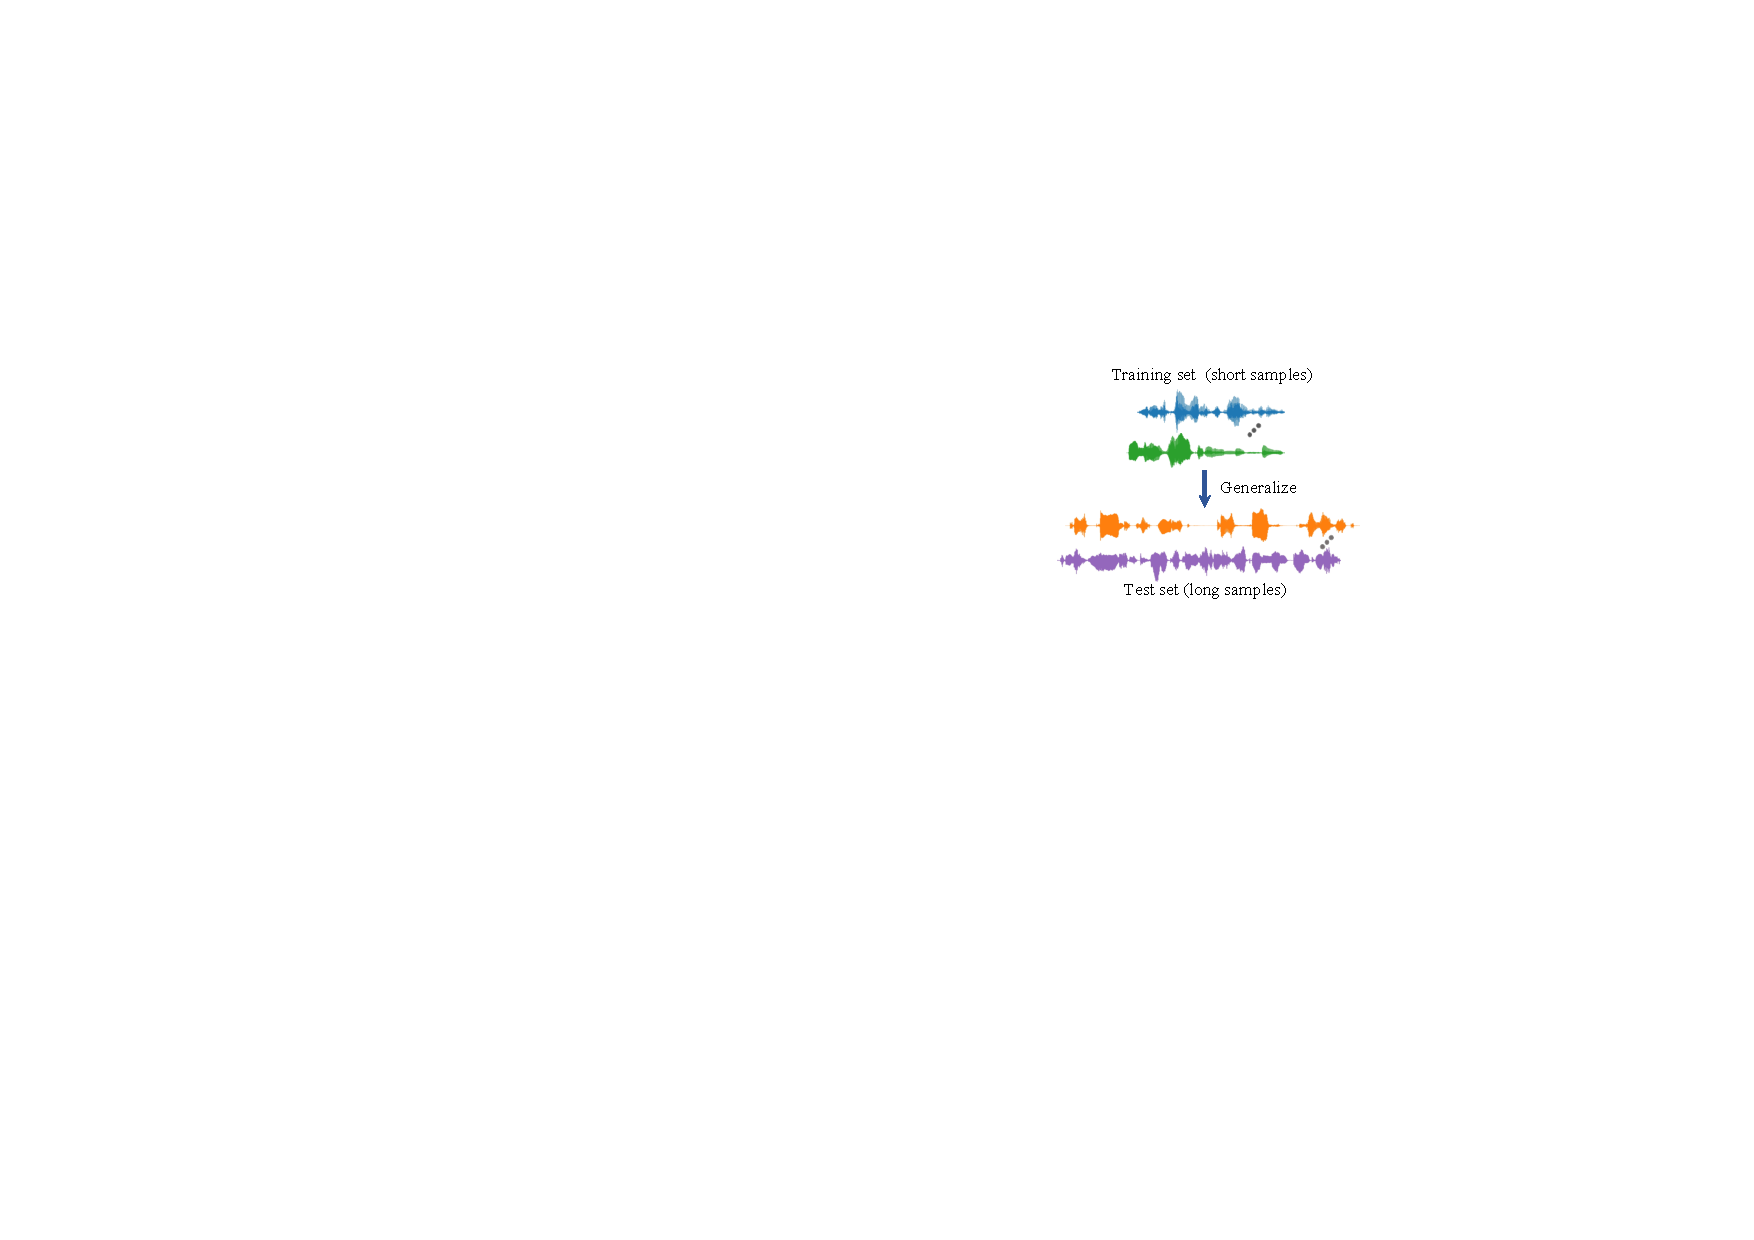
\includegraphics[width=0.81\columnwidth]{./diagram/Fig1.pdf}}
\caption{\textcolor{black}{Length generalization in speech enhancement: The ability to learn from short speech samples (training set) to generalize to longer speech samples (test set).} 
% \qian{The generalization ability to learn from short speech samples (training set) while inference on longer speech samples (test set)}
}
\label{generalize}
\vspace{-0.5em}
\end{figure}

\textcolor{black}{Monaural speech enhancement has been an active research direction in speech signal processing for decades, leading to the development of a variety of methods. Conventional speech enhancement techniques \cite{loizou} mainly involve spectral subtraction \cite{boll1979}, statistical model-based algorithms \cite{mmse,mmse2017,zhang2019}, and Wiener filtering \cite{wiener1996}. However, due to certain restrictions and simplifications about speech and noise characteristics, these algorithms often fail to eliminate fast-varying noise signals \cite{loizou}. In recent decades, facilitated by large-scale training data and powerful computing resources, deep learning technology has promoted enormous progress in speech enhancement \cite{overview2018,over2022}, demonstrating substantial performance improvements over conventional techniques.}

\textcolor{black}{Transformer network architectures have been widely used in speech and language processing. % across a wide range of natural language processing tasks. This inspires researchers to investigate the use of Transformers for speech processing, resulting in state-of-the-art performance in speech-related tasks, 
They have shown state-of-the-art performance in many speech processing tasks, such as speech enhancement \cite{cleanunet,mhanet,restcnsa,tgsa,zhao2020,ripple} and speech recognition \cite{conformer-asr}. The multi-head self-attention (MHSA) module is a core component in Transformers and explicitly learns the relevance of each time frame in a sequence with respect to all other time frames, generating context-informed feature representations. This enables Transformers to capture long-range temporal dependencies more efficiently.}

The generalization capability to unseen conditions during training is crucial for supervised learning tasks. In speech enhancement, generalization to unseen noise, speakers, and signal-to-noise ratios (SNRs) have been extensively studied. Besides the three aspects, the speech enhancement model is expected to generalize to perform on speech utterances significantly longer than those (usually with a fixed maximum length) seen during training. Self-attention suffers from the computation cost quadratic with respect to the sequence length, which makes it infeasible to use sufficiently long speech utterances for training Transformer. A natural question arises: ``Can the Transformer-based speech enhancement model effectively learn from shorter speech samples and generalize to longer ones?'', which is recently defined as the problem of length generalization \cite{anil2022exploring}. Aside from mitigating the computation cost issue, length generalization is an intriguing theoretical problem. 
In this paper, we extend our previous work~\cite{zhang2024exploration} by addressing issues how Transformer-based speech enhancement models handle long noisy speech samples. In Fig.~\ref{generalize}, we illustrate the concept of length generalization in speech enhancement.


% \qian{While no work explores the generalization to speech utterances that are significantly longer than those used during training, which usually have a fixed maximum length.}
% \qian{This mainly because ?}

% as illustrated in Figure \ref{generalize}.

% \qian{Indeed, length generalization not only affects the computation cost but also arises as an intriguing theoretical problem, as has been defined in\cite{anil2022exploring}.}

% See Figure \ref{generalize} for an illustrative example of length generalization in speech enhancement.
% explore how to enable the Transformer-based speech enhancement model to perform length generalization. 



% \textcolor{black}{The generalization capability to conditions unseen during training is critical in a supervised learning task. For speech enhancement, the generalizations to unseen noise, speakers, and signal-to-noise ratios (SNRs) are three important aspects, which have been extensively studied. However, aside from the three aspects, in practical scenarios, one desires speech enhancement models are also often asked to continue to perform well on speech utterances significantly longer than ones encountered during training. A straightforward way to address this issue is to include speech utterances with a variety of lengths for training the model. However, self-attention operation suffers from the computation cost quadratic with respect to the sequence length, which makes it often infeasible to use sufficiently long speech utterances for training. A natural question arises: ``Can the Transformer-based speech enhancement model learn from shorter speech samples to generalize longer ones?'', which is recently defined as the problem of length generalization \cite{anil2022exploring}. Aside from the issue of computation cost, it is also an intriguing theoretical problem. In this study, we explore how to enable the Transformer-based speech enhancement model to perform length generalization. See Fig. \ref{generalize} for an illustrative example of length generalization in speech enhancement.}

% on speech utterances with a variety of lengths

In the vanilla Transformer formula~\cite{attention2017}, a sinusoidal position embedding is used to allow the model to handle sequences of variable length between training and testing. However, we observe that such position embedding is not effective. Studies have shown that relative position encoding (RPE) schemes exhibit a better generalization property, e.g., T5-Bias~\cite{T5}, TISA~\cite{tisa}, and KERPLE~\cite{kerple}. We are inspired by RPE to enable Transformer-based speech enhancement for length generalization at run-time.

\textcolor{black}{In this paper, we explore seven existing positional encoding methods in length generalization.} 
% \textcolor{red}{Since these methods are not initially designed for speech tasks, their constraints to learn the position-aware
% bias may not be optimal for the speech enhancement task.}
These methods are initially designed for natural language processing. Note that speech spectrogram has a more rigid temporal order than text tokens in natural language. We argue that the complex formulations for positional encoding in T5-Bias, KERPLE, and TISA may not be effective for speech tasks. Hence, we attempt to explore a more efficient RPE scheme with a simpler design, i.e., LearnLin, which encodes position information by exploiting only one learnable parameter to explicitly scale the relative distance between different time frames. A different parameter is learned for each attention head, which adjusts the preferences of different heads on short- or long-range temporal dependencies. It biases the raw attention scores with summation operation before Softmax normalization. \textcolor{black}{In summary, this paper extends the previous work~\cite{zhang2024exploration} with the following contributions:}

% In summary, \textcolor{blue}{the main contributions of this paper to the previous work~\cite{zhang2024exploration} are as follows:}

% 2. I would like to acknowledge that the journal submission (T-ASL-11388-2024) is indeed an extension of our INTERSPEECH 2024 paper.  However, the journal submission extended the previous work by studying the length generalization capabilities of Transformer-based speech enhancement models, with the following novel contributions: 

% \qian{can we move this phara to Sec. II?}
% \begin{itemize}
%     \item \textcolor{red}{To the best of our knowledge, the length generalization problem of Transformer-based speech enhancement model has not been explored. We show the issues or pathologies that arise when the Transformer model processing long noisy inputs.}
%     % We present a new form of out-of-distribution generalization in supervised speech enhancement, i.e., length extrapolation.
%     \item \textcolor{red}{We explore several advanced positional encoding methods to dampen the effect of utterance length across causal and non-causal configurations. Our findings establish that relative position encoding (RPE) yields better length generalization capability than absolute position encoding (APE).}
%     % \item We show that much simpler position-aware attention bias that scales the relative position between time frames with a learnable parameter
%     \item \textcolor{red}{We also explore a simpler and more efficient positional encoding scheme (LearnLin) for Transformer speech enhancement, which employs only one trainable parameter in each head to scale the relative distance to learn the preferences on long- or short-term dependencies. Experiments show that LearnLin is superior or on par with other prior models in terms of length generalization. The performance superiority of over chunk processing underscores the importance of length generalization.}
% \end{itemize}
% Comprehensive experiments

\begin{itemize}
    \item \textcolor{black}{We explore a simpler and more efficient positional encoding scheme (LearnLin) for Transformer speech enhancement, which employs only one trainable parameter in each head to scale the relative distance to learn the preferences on long- or short-term dependencies. Experiments show that LearnLin is superior or on par with other prior models in terms of length generalization.}
    
    \item \textcolor{black}{We conduct a more comprehensive and systematic exploration of seven positional encoding approaches on four training targets (including both mapping- and masking-based methods) to dampen the effect of utterance length, across both causal and non-causal model configurations. 
    % Our findings establish that relative position encoding (RPE) yields better length generalization capability than absolute position encoding (APE).
    }
    % \item We show that much simpler position-aware attention bias that scales the relative position between time frames with a learnable parameter
    \item \textcolor{black}{We further evaluate the performance under chunk-based processing, both without overlap and with a 50\% overlap. The results highlight the effectiveness and importance of performing length generalization.}
\end{itemize}

\textcolor{black}{The remainder of this paper is structured as follows. In Section~\ref{sec:2}, we describe related works, including speech enhancement and length generalization. Section~\ref{sec:3} elaborates on the positional encoding methods. Section~\ref{sec:4} formulates the research problem. \textcolor{black}{In Section~\ref{sec:5}, we describe speech enhancement with position-aware Transformer Section~\ref{sec:6} describes the experimental setup. The experimental results are presented in Section~\ref{sec:7}. Finally, Section~\ref{sec:8} concludes this study.}}

% \textcolor{black}{The remainder of this paper is structured as follows. In Section \ref{sec:2}, we review the positional encodings. Section \ref{sec:3} formulates the research problem. In Section \ref{sec:3}, we propose a novel time-frequency attention mechanism for speech enhancement. In Section \ref{sec:4}, we describe the experimental setup. The experimental results are presented in Section \ref{sec:5}. Finally, Section \ref{sec:6}  concludes  this study.}


\section{Related Work} \label{sec:2}
% \subsection{Speech Enhancement}
\textcolor{black}{Neural speech enhancement schemes can be grouped into waveform-domain methods and time-frequency (T-F) domain methods. The waveform-domain methods recover the target speech in an end-to-end manner by optimizing a deep neural network (DNN) model to directly predict the raw waveform of the clean speech from the noisy one~\cite{SEGAN,2017raw, kolbaek2020loss,2018raw,demcus,cleanunet}. Many other speech enhancement techniques are carried out in a time-frequency (T-F)  domain~\cite{overview2018,over2022}, such as spectral mapping and T-F masking methods. Spectral mapping methods optimize the DNN model to map the T-F representation (or spectral feature) of the noisy speech to the clean T-F representation. The most commonly used spectral features for spectral mapping include log-power spectrum (LPS)~\cite{yongxu2015}, magnitude spectrum (MS)~\cite{crn2018,GRN,restcnsa,sa-tcn}, and complex spectrum (CS)~\cite{2018complex,tan2019learning}. In T-F masking methods, the DNN model is trained to predict a T-F mask, which is then applied to the noisy T-F representation to obtain the clean one. Furthering the idea of auditory T-F masking, the ideal binary mask (IBM) is proposed as the training objective to accomplish speech enhancement, where the speech- and noise-dominated T-F units are labeled as one and zero, respectively~\cite{wang2013}. Later, different types of T-F masks are developed along this line of research, where the most popular ones include the spectral magnitude mask (SMM)~\cite{targets}, ideal ratio mask (IRM) \cite{targets}, complex ideal ratio mask (cIRM)~\cite{cirm}, and phase-sensitive mask (PSM)~\cite{psm}.}

\textcolor{black}{
% Effective speech enhancement algorithms rely on a well-designed backbone network architecture. 
Initial speech enhancement models typically employ a feed-forward DNN (FNN) as the backbone network, which can only leverage limited temporal correlations provided by a sliding window of consecutive time frames~\cite{yongxu2015,targets,cirm}. Later, with the capability to effectively exploit the long-range temporal dependencies present in speech signals, the long short-term memory (LSTM) recurrent neural networks (RNNs) exhibit significant performance superiority over FNNs and generalize well to speakers unseen during training~\cite{2014lstm,2015lstm,chenlstm}. Nevertheless, deep RNN-LSTM architectures involve a large number of parameters, meanwhile, the parallelization of computation is impaired due to the inherent sequential nature of RNNs, which excludes its use in many applications. Instead of the frame-wise sequential prediction in RNNs, convolutional neural networks (CNNs) process an input sequence of time frames in parallel. Recently, a one-dimensional (1D) fully convolution network termed the residual temporal convolutional network (ResTCN) employs a deep stack of residual blocks comprised of dilated 1D convolution layers to build a very large receptive field, demonstrating impressive capability in capturing long-range temporal dependencies. ResTCNs have been reported to yield comparable or better results than RNNs on a number of sequence modeling problems, with significantly faster training speed and less parameter overhead~\cite{TCN2018}. ResTCNs have recently been applied to speech enhancement~\cite{GRN,DeepMMSE,tfa} and speaker separation~\cite{zhiqiang2019,convtasnet} with considerable success. More recently, Transformer network architecture, which employs the self-attention mechanism to enable the model to capture long-term dependencies more efficiently, has established state-of-the-art results in numerous speech processing tasks, including speech enhancement~\cite{tgsa,tfaj,conformer-se,dang2022dpt,yu2022dual}.}


% ResTCNs employ a deep stack of residual blocks comprised of dilated one-dimensional (1D) convolution layers to build a very large receptive field, demonstrating impressive capability in capturing long-range temporal dependencies.

% \textcolor{blue}{Effective speech enhancement algorithms rely on a well-designed backbone network architecture. Initial speech enhancement models employ a feed-forward DNN (FNN) as the backbone network, which can only leverage limited temporal correlations provided by a sliding window of successive time frames~\cite{yongxu2015,targets,cirm}. With the ability to effectively model the long-range temporal dependencies present in speech signals, long short-term memory (LSTM) recurrent neural networks (RNNs) are exploited for speech enhancement \cite{2014lstm,2015lstm,chenlstm}. The LSTM-RNN models exhibit significant performance gains over FNNs and generalize well to speakers unseen during training \cite{chenlstm}. Nevertheless, deep LSTM-RNN architectures require a large size of parameters and do not allow parallel computation due to the inherently sequential nature of RNNs, which excludes its use in many applications. Instead of the frame-wise sequential prediction in RNNs, convolutional neural networks (CNNs) process an input sequence of time frames in parallel. A residual temporal convolution network (ResTCN) \cite{TCN2018} builds a sufficiently large receptive field by stacking residual blocks that consist of dilated 1-D convolution layers, exhibiting excellent capability in capturing long-range temporal dependencies. ResTCNs have shown promising results in a number of tasks on sequence modeling \cite{TCN2018} and have recently been applied to speech enhancement \cite{GRN,DeepMMSE,tfa,senet} and speaker separation \cite{convtasnet} with considerable success.}


% \textcolor{black}{Self-attention based Transformer network architectures have been dominant across a wide range of natural language processing tasks. It inspires researchers to investigate the use of Transformers for speech processing, where Transformers have recently demonstrated state-of-the-art results in many speech tasks including speech enhancement \cite{cleanunet,mhanet,restcnsa,tgsa,zhao2020} and speech recognition \cite{conformer-asr}. As the core component in Transformers, the multi-head self-attention (MHA) module explicitly learns the relevance of each time frame with respect to all time frames in a sequence to generate the context-informed feature representations, enabling Transformers to capture long-range temporal dependencies more efficiently.}

% \textcolor{black}{The generalization capability to conditions unseen during training is critical in a supervised learning task. For speech enhancement, the generalizations to unseen noise, speakers, and signal-to-noise ratios (SNRs) are three important aspects, which have been extensively studied in recent years. Aside from the three aspects, in practical scenarios, speech enhancement models are also inevitably required to continue to perform well on speech utterances significantly longer than ones encountered during training. A straightforward way to address this issue is to train the model on speech utterances with a variety of lengths. However, self-attention operation suffers from the computation cost quadratic with respect to the sequence length, which makes it often infeasible to use sufficiently long speech utterances for training. \textcolor{blue}{A natural question arises: ``Can the Transformer-based speech enhancement model learn from shorter speech samples to generalize longer ones?'', which is recently defined as the problem of length generalization \cite{anil2022exploring}. In this study, we explore how to enable the Transformer-based speech enhancement model to perform length generalization. See Fig. \ref{generalize} for an illustrative example of length generalization in speech enhancement.
% }}

% \textcolor{black}{A line of research investigates efficient Transformer architectures for speech enhancement.}

% In this paper, we explore how to enable the Transformer-based speech enhancement model with the length generalization capability to learn from shorter speech samples to generalize longer ones. See Fig. \ref{generalize} for an illustrative example of length generalization in speech enhancement. \textcolor{black}{The original Transformer work \cite{attention2017} introduces the sinusoidal position encoding and speculates that it may allow the model to generalize to sequences longer than that at training time. However, we observe that the sinusoidal position encoding lacks the generalization property. It is suggested that relative position encoding (RPE) schemes exhibit a better generalization property, e.g., T5 bias \cite{T5}, TISA \cite{tisa}, and KERPLE \cite{kerple}. We are inspired to explore RPE to allow Transformer-based speech enhancement to perform length generalization at runtime. This study proposes an efficient RPE method, which encodes position information by exploiting a learnable parameter to explicitly scale the relative distance between different time frames. A different parameter is learned for each attention head, which adjusts the heads tend to focus on short or distant relations. It biases the raw attention scores with summation operation before Softmax normalization. The main contributions of this paper are as follows:}

% \textcolor{black}{The original Transformer publication \cite{attention2017} introduces the sinusoidal position encoding and hypothesizes that it may allow the model to generalize to sequences longer than that at training time. However, we observe that the sinusoidal position encoding lacks the generalization property. It is suggested that relative position encoding (RPE) schemes exhibit a better generalization property, e.g., T5-Bias \cite{T5}, TISA \cite{tisa}, and KERPLE \cite{kerple}. We are inspired to explore RPE to enable Transformer-based speech enhancement to perform length generalization at runtime. 
% This study explores several prior methods and presents a more efficient RPE method, which encodes position information by exploiting a learnable parameter to explicitly scale the relative distance between different time frames. A different parameter is learned for each attention head, which adjusts the heads tend to focus on short or distant relations. It biases the raw attention scores with summation operation before Softmax normalization. The main contributions of this paper are as follows:}

% \begin{itemize}
%     \item To the best of our knowledge, we are the first to formulate and explore the length generalization or extrapolation problem in Transformer\qian{-based} speech enhancement.
%     % We present a new form of out-of-distribution generalization in supervised speech enhancement, i.e., length extrapolation.
%     \item We explore the length generalization ability of several existing positional encoding methods in Transformer-based speech enhancement. Our findings show that relative positional encoding schemes yield better length generalization capacity than absolute positional encoding.
%     \item We present a simple yet effective position-aware attention bias for speech enhancement, which scales the relative position between time frames with a learnable parameter.
%     \item Comprehensive experiments show that the proposed position encoding method can \qian{achieve comparable or even superior} length generalization than state-of-the-art methods.
% \end{itemize}

% \textcolor{black}{The remainder of this paper is structured as follows. In Section \ref{sec:2}, we review the positional encodings. Section \ref{sec:3} formulates the research problem. In Section \ref{sec:3}, we propose a novel time-frequency attention mechanism for speech enhancement. In Section \ref{sec:4}, we describe the experimental setup. The experimental results are presented in Section \ref{sec:5}. Finally, Section \ref{sec:6}  concludes  this study.}


% \textcolor{blue}{Various DNN architectures have been explored for speech enhancement. Initial speech enhancement models employed a feed-forward DNN (FNN) as the backbone network, such as \cite{yongxu2015,targets,cirm,tms2015}. In the study \cite{2015lstm}, speech enhancement is formulated as a sequence-to-sequence mapping and a long short-term memory (LSTM) recurrent neural network (RNN) architecture is utilized to model the long-term dependencies present in speech signals. The RNN-LSTM architecture exhibit significant performance gains over FNNs \cite{chenlstm,2014lstm,2015lstm}.}


% {Early speech enhancement models typically employ a feed-forward DNN (FNN) as the backbone network. Due to the ability to model the long-term dependencies present in speech signals, recurrent neural networks (RNNs) with long short-term memory (LSTMs) are employed for speech enhancement task, exhibiting significant performance gains over FNNs.
% }


% {Speech signals in a real-world acoustic environment are inevitably corrupted by background noise, which can severely degrade speech quality and intelligibility. Speech enhancement seeks to separate the target speech signal from the background noise. It is an essential component in a number of speech processing systems, such as hearing aids, automatic speech recognition (ASR), speaker verification, and brain-computer interface. Monaural speech enhancement represents one of the challenges. Traditional signal processing-based methods have been extensively studied for a long time, mainly including spectral subtraction \cite{boll1979}, Wiener filtering \cite{wiener1996}, and statistical model-based methods \cite{mmse,mmse2017,zhang2019}. These methods perform well for stationary noise, however, fail to handle non-stationary noise.} 

% \subsection{Length Generalization}
% \textcolor{black}{To the best of our knowledge, the problem of length generalization has not yet been investigated in speech enhancement. There have been attempts to explore it with Transformers in language modeling \cite{kerple,alibi,anil2022exploring}, machine translation, and image recognition \cite{likhomanenko2021cape}. Anil \textit{et al.} \cite{anil2022exploring} show that few-shot scratchpad prompting results in a considerable improvement for pre-trained large language models in length generalization. Press \textit{et al.} \cite{alibi} propose an RPE method termed ALiBi that employs fixed slopes to weight the real relative distance to enable the length generalization. Later, Chi \textit{et al.} \cite{kerple} propose the kernelized relative positional embedding (KERPLE), which demonstrates that ALiBi is a particular instance of KERPLE and achieves better generalization performance \cite{kerple}. It is worth noting that both of the methods are limited to causal language modeling. Here, we do not constrain our speech enhancement system to be causal. A recent study \cite{yehudai2021local} explores the ability of graph neural networks (GNNs) to generalize from small to large graphs.}

\textcolor{black}{To the best of our knowledge, the problem of length generalization has not yet been investigated in Transformer-based speech enhancement. There have been attempts to explore it with Transformers in language modeling \cite{kerple,alibi,anil2022exploring}, machine translation, and image recognition \cite{likhomanenko2021cape}. Anil \textit{et al.} \cite{anil2022exploring} define the length generalization problem and establish that few-shot scratchpad prompting leads to a considerable improvement for pre-trained large language models (LLMs) in length generalization. Press \textit{et al.} \cite{alibi} propose an RPE method termed ALiBi that employs fixed slopes to weight the real relative distance to enable the length generalization for causal language modeling. Later, Chi \textit{et al.} \cite{kerple} propose the kernelized relative position embedding (KERPLE), which demonstrates that the ALiBi is a particular instance of KERPLE and achieves superior generalization performance \cite{kerple} in perplexity. Dubois \textit{et al.} \cite{dubois2020location} present a novel location-based attention to facilitate generalization to longer sequences. Newman \textit{et al.} \cite{newman2020extrapolation} find that generative language models trained to predict the end-of-sequence (EOS) token exhibit worse length generalization ability than those not trained to predict the EOS token. A recent work \cite{yehudai2021local} investigates the capability of graph neural networks (GNNs) to generalize from small to large graphs.}


% The length generalization problem is also present in graph neural networks (GNNs) learning \cite{yehudai2021local}. 
% where generalization from small to large graphs is challenging.

% Existing positional encoding methods in Transformers, which can be divided into two groups: absolute positional encoding (APE) and relative positional encoding (RPE).

% \subsubsection{Absolute Position Encoding}

% \textcolor{black}{APE methods assign a unique positional vector to each time step, which is then summed with the input frame embedding to form the input to the first Transformer layer. APE involves two types of encoding techniques: constant and learnable \cite{bert}.}

% \textbf{Sinusoidal Position Embeddings}. \textcolor{black}{The original Transformer paper considers the APE and proposes the sinusoidal positional embeddings \cite{attention2017} that are fixed and non-learned vectors calculated using the deterministic functions, i.e., cosine and sine functions. Specifically, for the $l$-th time frame, the $d$-th component of position embedding $E_{l,d}$ is given as: }
% \begin{equation}
% E_{l,d}\!=
% \begin{cases}
% \sin\left(l \cdot 10000^{-\frac{d}{d_\text{model}}}\right), & d \text{ is even } \\
% \cos\left(l \cdot 10000^{-\frac{d-1}{d_\text{model}}} \right), & d \text{ is odd }
% \end{cases}
% \end{equation}
% \textcolor{black}{where $d_\text{model}$ denotes the dimension of the input embeddings. It is a commonly used position encoding method in Transformer-based speech enhancement and speaker separation as well.}

% \textbf{Learnable Absolute Position Embeddings}. BERT \cite{bert} replaces the fixed sinusoidal position embeddings with absolute learned position embeddings $\mathbf{E}\!\in\!\mathbb{R}^{L \times d_\text{model}}$ corresponding to the time frames $l=1,2,...,L$ in an utterance. Here we refer to the learned APE as ``BERT-Pos.''.

% \subsubsection{Relative Position Encoding}
% \textcolor{black}{APE is restricted to fixed max sequence lengths. Instead of encoding absolute positions, RPE directly considers relative distances between two elements in a sequence.}

% \textbf{Gaussian Bias} \textcolor{black}{(Gauss-Bias) \cite{gaussbias} encodes relative positions through a Gaussian function, where the relative distance between $i$-th and $j$-th time frames is encoded as:}
% \begin{equation}
% P_{i,j}=\frac{-(i-j)^2}{2 \sigma^2}
% \end{equation}
% \textcolor{black}{where $\sigma$ denotes a trainable standard deviation parameter. Different parameters are learned for each attention head, and parameters are shared across layers.}

% \textbf{T5-Bias}. 
% % \textcolor{black}{The T5 model \cite{T5} injects position information by summing the scalar relative position embeddings with the attention weights matrix, where the relative position embeddings are shared across layers. The relative positions are split into a fixed number of buckets with a log-binning strategy and the positions in the same bucket share the same position embedding. We refer to this RPE method as ``T5-Bias''. To be specific, given a bucket of $32$ learnable parameters $\textbf{B}$, for each attention head, the scalar position embeddings $P_{i,j}$ are extracted from the bucket with the following rule: }
% \textcolor{black}{In the T5 model \cite{T5}, the relative positions are split into a fixed number of buckets with a log-binning strategy and the positions in the same bucket share the same position embedding. The relative position embeddings are shared across layers. To be specific, given a bucket of $32$ learnable parameters $\textbf{B}$, for each attention head, the scalar position embeddings $P_{i,j}$ are extracted from the bucket with the following rule: }
% \begin{equation}
% P_{i,j}\!=\! 
% \begin{cases}
% \textbf{B}[\min(15,8\!+\!\lfloor\frac{\log ((|i-j|)/8)}{\log(128/8)} \cdot 8\rfloor)\!+\!16], \quad i\!-\!j \!\leq\! -8 \\
% \textbf{B}[|i-j|+16], \qquad \qquad \qquad \qquad \quad \, \!{-8}\!<\! i\!-\!j\!<\!0\\ 
% \textbf{B}[i-j], \qquad \qquad \qquad \qquad \qquad \qquad \,\,\, 0\!\leq\!i\!-\!j\!<\!8\\ 
% \textbf{B}[\min(15,8\!+\!\lfloor\frac{\log ((i-j) / 8)}{\log (128 / 8)} \cdot 8\rfloor)], \qquad \qquad i\!-\!j\!\geq\! 8
% \end{cases}
% \end{equation}
% \textcolor{black}{Where $\lfloor\cdot\rfloor$ denotes the floor function. We refer to this RPE method as ``T5-Bias''.}

% \textbf{Translation-Invariant Self-Attention (TISA) Bias}. \textcolor{black}{The TISA model \cite{tisa} encodes relative positions using  radial-basis functions shaped by several trainable parameters, which provides both localized and global attention, defined as:}

% \begin{equation}
% P_\theta(i,j)=\sum_{s=1}^S a_s \exp \left(-\left|b_s\right|\left(j-i-c_s\right)^2\right)
% \end{equation}
% \textcolor{black}{where $\theta\!=\!\left\{a_s, b_s, c_s\right\}_{s=1}^S$ denote the trainable parameters, where three parameters are included for each kernel $s$. Every attention head and layer employs different parameters. We refer to this position encoding method as the ``TISA''.}

% \textbf{DA-Bias}. The distance-aware Transformer \cite{DA} employs a learnable sigmoid function to encode the relative position (referred to as ``DA-Bias''), given as:
% \begin{equation}
%     P_{i,j} = \frac{1+\text{exp}(v)}{1+\text{exp}(v-(w|i-j|))}
% \end{equation}
% where $w$ and $v$ denote two learnable parameters for each head that are used to scale the relative distance and control the upper bound and ascending steepness of the function, respectively. 

% \textbf{KERPLE} \cite{kerple} learns the relative position embedding with conditionally positive definite kernels and proposes the power variant and the logarithmic variant, where the logarithmic variant achieves better performance, given as:
% \begin{equation}
%     P_{i,j} = -r_{1}\cdot \text{log}(1+r_{2}|i-j|)
% \end{equation}
% where $r_{1}>0$ and $r_{2}>0$ are two learnable parameters for each head.

% Among these RPE methods, except for DA-Bias that injects position information with multiplication operation (equation (6) in \cite{DA}), the other RPE methods inject position information by summing the relative position embeddings with the raw attention weights matrix.

% % \textbf{Length Generaliazation}. \textcolor{blue}{To our best knowledge, the length generalization has not been previously studied in Transformer-based speech enhancement model, but there have been attempts to explore it with Transformers in language modeling \cite{kerple,alibi,anil2022exploring}, machine translation, and image recognition \cite{likhomanenko2021cape}. Anil \textit{et al.} \cite{anil2022exploring} show that few-shot scratchpad prompting leads to a considerable improvement for pre-trained large language models in length generalization. Chi \textit{et al.} \cite{kerple} propose kernelized relative positional embedding (KERPLE) to enable length generalization and demonstrate that the attention bias (ALiBi) \cite{alibi} is a particular instance of KERPLE. 
% % Press \textit{et al.} \cite{alibi} propose an RPE method (called ALiBi) that employs fixed slopes to scale the relative distance to enable the Transformer language model with the length generalization ability. Later, KERPLE demonstrates that ALiBi is a particular instance of KERPLE and achieves better generalization property \cite{kerple}. It is worth noting that both ALiBi and KERPLE are limited to causal language modeling. Here we do not constrain our model to be causal. 
% % }

% \textbf{Length Generaliazation}. \textcolor{blue}{To our best knowledge, the length generalization has not been previously studied in Transformer-based speech enhancement model, but there have been attempts to explore it with Transformers in language modeling \cite{kerple,alibi,anil2022exploring}, machine translation, and image recognition \cite{likhomanenko2021cape}. Anil \textit{et al.} \cite{anil2022exploring} show that few-shot scratchpad prompting results in a considerable improvement for pre-trained large language models in length generalization. Press \textit{et al.} \cite{alibi} propose an RPE method (called ALiBi) that employs fixed slopes to scale the relative distance to enable the length generalization. Later, Chi \textit{et al.} \cite{kerple} propose kernelized relative positional embedding (KERPLE), which demonstrates that ALiBi is a particular instance of KERPLE and achieves better generalization property \cite{kerple}. It is worth noting that both of the methods are limited to causal language modeling. Here we do not constrain our model to be causal. }

\section{\textcolor{black}{Positional Encoding}} \label{sec:3}
% \qian{We start by elaborating }
\textcolor{black}{Existing positional encoding methods in Transformers can be divided into two groups: absolute position encoding (APE) and relative position encoding (RPE).}

\subsection{Absolute Positional Encoding}

\textcolor{black}{APE methods assign a unique position vector or embedding to each time step, which is then summed with the input frame embedding to form the input to the first Transformer layer. APE involves two types of encoding techniques: constant \cite{attention2017} and learnable \cite{bert}.}

\textbf{Sinusoidal Position Embedding}. The original Transformer paper proposes the sinusoidal position embeddings \cite{attention2017} that are fixed and non-learned vectors calculated using the deterministic functions, i.e., cosine and sine functions. Specifically, for the $l$-th time frame, the $d$-th component of position embedding $E_{l,d}$ is given as: 
\begin{equation}
% \setlength{\abovedisplayskip}{2pt}
% \setlength{\belowdisplayskip}{2pt}
E_{l,d}\!=
\begin{cases}
\sin\left(l \cdot 10000^{-\frac{d}{d_{model}}}\right), & d \text{ is even } \\
\cos\left(l \cdot 10000^{-\frac{d-1}{d_{model}}} \right), & d \text{ is odd }
\end{cases}
\end{equation}
\textcolor{black}{where $d_{model}$ denotes the dimension of the input embedding. It is a commonly used positional encoding scheme in Transformer-based speech enhancement \cite{sepformerstft} and speaker separation \cite{sepformer} as well.}

\textbf{Learnable Absolute Position Embedding}. BERT \cite{bert} replaces the fixed sinusoidal position embeddings with fully-learnable absolute position embeddings $\mathbf{E}\!\in\!\mathbb{R}^{L \times d_\text{model}}$ corresponding to the time frames $l=1,2,...,L$ in an utterance. Here we refer to the learnable APE as ``BERT-Pos''.

\subsection{Relative Positional Encoding}\label{sec:3.2}

\textcolor{black}{APE is restricted to fixed max sequence lengths. Instead of encoding absolute positions, RPE considers relative distances between two elements in a sequence.}

\textbf{Gaussian Bias} \textcolor{black}{(Gauss-Bias) is proposed for acoustic modeling in \cite{gaussbias}, which encodes the relative position through a Gaussian function, where the relative position between $i$-th and $j$-th time frames is encoded as:}
\begin{equation}\label{gauss-bias}
P_{i,j}=\frac{-(i-j)^2}{2 \sigma^2}
\end{equation}
\textcolor{black}{where $\sigma$ denotes a trainable standard deviation parameter. Different parameters are learned for each attention head, and parameters are shared across layers. 
}

\textbf{T5-Bias}. 
% \textcolor{black}{The T5 model \cite{T5} injects position information by summing the scalar relative position embeddings with the attention weights matrix, where the relative position embeddings are shared across layers. The relative positions are split into a fixed number of buckets with a log-binning strategy and the positions in the same bucket share the same position embedding. We refer to this RPE method as ``T5-Bias''. To be specific, given a bucket of $32$ learnable parameters $\textbf{B}$, for each attention head, the scalar position embeddings $P_{i,j}$ are extracted from the bucket with the following rule: }
\textcolor{black}{In T5 model \cite{T5}, the relative positions $i-j$ are split into a fixed number of buckets with a log-binning strategy and the positions in the same bucket share the same position embedding. The relative position embedding or bias is shared across layers. To be specific, given a bucket of $32$ learnable parameters $\textbf{B}$, for each attention head, the scalar position bias $P_{i,j}$ is extracted from the bucket with the following rule: }
\begin{equation}
P_{i,j}\!=\! 
\begin{cases}
\textbf{B}[\min(15,8\!+\!\lfloor\frac{\log ((|i-j|)/8)}{\log(128/8)} \cdot 8\rfloor)\!+\!16], \quad i\!-\!j \!\leq\! -8 \\
\textbf{B}[|i-j|+16], \qquad \qquad \qquad \qquad \quad \, \!{-8}\!<\! i\!-\!j\!<\!0\\ 
\textbf{B}[i-j], \qquad \qquad \qquad \qquad \qquad \qquad \,\,\, 0\!\leq\!i\!-\!j\!<\!8\\ 
\textbf{B}[\min(15,8\!+\!\lfloor\frac{\log ((i-j) / 8)}{\log (128 / 8)} \cdot 8\rfloor)], \qquad \qquad i\!-\!j\!\geq\! 8
\end{cases}
\end{equation}
\textcolor{black}{Where $\lfloor\cdot\rfloor$ denotes the floor function. We refer to this RPE method as ``T5-Bias''.}

\textbf{Translation-Invariant Self-Attention (TISA)}. \textcolor{black}{The TISA model \cite{tisa} encodes relative positions using radial-basis functions shaped by several trainable parameters, which provides both localized and global attention, defined as:}

\begin{equation}
{P_{i,j}=\sum_{s=1}^S a_s \exp \left(-\left|b_s\right|\left(j-i-c_s\right)^2\right)}
\end{equation}
{where $a_s$, $b_s$, and $c_s$ denote the three trainable parameters included for each kernel $s\!\in\!\left\{1,...,S\right\}$.} Every attention head and layer employs different parameters. We refer to this positional encoding method as the ``TISA''. %\textcolor{red}{(I suggest changing $P_\theta(i,j)$ to $P_{i,j}$)} \textcolor{blue}{To Prof. Li, I have revised it.}

% $\theta\!=\!\left\{a_s, b_s, c_s\right\}_{s=1}^S$
\textbf{DA-Bias}. The distance-aware Transformer \cite{DA} employs a learnable sigmoid function to encode the relative position (referred to as ``DA-Bias''), given as:
\begin{equation}\label{dabias}
    P_{i,j} = \frac{1+\text{exp}(v)}{1+\text{exp}(v-(w|i-j|))}
\end{equation}
where $w$ and $v$ denote two learnable parameters for each head that are used to scale the relative distance and control the upper bound and ascending steepness of the function, respectively. 

\textbf{KERPLE} \cite{kerple} learns the relative position embedding with conditionally positive definite kernels, including the power variant and the logarithmic variant, where the logarithmic variant achieves better performance, given as:
\begin{equation}\label{kerple}
    P_{i,j} = -r_{1}\cdot \text{log}(1+r_{2}|i-j|)
\end{equation}
where $r_{1}>0$ and $r_{2}>0$ are two learnable parameters for each head. Note KERPLE is limited to causal language modeling. Here, we do not constrain our speech enhancement system to be causal.

\textcolor{black}{Among the aforementioned RPE methods}, except for DA-Bias which injects the position information with multiplication operation, the other RPE methods inject position information by adding the relative position embeddings (or bias) with the raw attention scores matrix.

\textcolor{black}{\textbf{Rotary Position Embedding (RoPE)}. The RoPE~\cite{RoPE} injects position information by rotating key and query representations with angles proportional to their absolute positions in each self-attention layer. With this rotation, the attention dot product exhibits the explicit relative position dependency. We refer readers to the original publication~\cite{RoPE} for more details.}

% \textbf{Length Generaliazation}. \textcolor{blue}{To our best knowledge, the length generalization has not been previously studied in Transformer-based speech enhancement model, but there have been attempts to explore it with Transformers in language modeling \cite{kerple,alibi,anil2022exploring}, machine translation, and image recognition \cite{likhomanenko2021cape}. Anil \textit{et al.} \cite{anil2022exploring} show that few-shot scratchpad prompting leads to a considerable improvement for pre-trained large language models in length generalization. Chi \textit{et al.} \cite{kerple} propose kernelized relative positional embedding (KERPLE) to enable length generalization and demonstrate that the attention bias (ALiBi) \cite{alibi} is a particular instance of KERPLE. 
% Press \textit{et al.} \cite{alibi} propose an RPE method (called ALiBi) that employs fixed slopes to scale the relative distance to enable the Transformer language model with the length generalization ability. Later, KERPLE demonstrates that ALiBi is a particular instance of KERPLE and achieves better generalization property \cite{kerple}. It is worth noting that both ALiBi and KERPLE are limited to causal language modeling. Here we do not constrain our model to be causal. 
% }

% \textbf{Length Generaliazation}. \textcolor{blue}{To our best knowledge, the length generalization has not been previously studied in Transformer-based speech enhancement model, but there have been attempts to explore it with Transformers in language modeling \cite{kerple,alibi,anil2022exploring}, machine translation, and image recognition \cite{likhomanenko2021cape}. Anil \textit{et al.} \cite{anil2022exploring} show that few-shot scratchpad prompting results in a considerable improvement for pre-trained large language models in length generalization. Press \textit{et al.} \cite{alibi} propose an RPE method (called ALiBi) that employs fixed slopes to scale the relative distance to enable the length generalization. Later, Chi \textit{et al.} \cite{kerple} propose kernelized relative positional embedding (KERPLE), which demonstrates that ALiBi is a particular instance of KERPLE and achieves better generalization property \cite{kerple}. It is worth noting that both of the methods are limited to causal language modeling. Here we do not constrain our model to be causal. }



% \IEEEPARstart{S}{peech} signals in a real-world acoustic environment are inevitably corrupted by background noise, which can severely degrade speech quality and intelligibility. Speech enhancement seeks to separate the target speech signal from the background noise. It is an essential component in a number of speech processing systems, such as hearing aids, automatic speech recognition (ASR), speaker verification, and brain-computer interface. Monaural speech enhancement represents one of the challenges. Traditional signal processing-based methods have been extensively studied for a long time, mainly including spectral subtraction \cite{boll1979}, Wiener filtering \cite{wiener1996}, and statistical model-based methods \cite{mmse,mmse2017,zhang2019}. These methods perform well for stationary noise, however, fail to handle non-stationary noise. 


% With the advent of deep learning, speech enhancement has made remarkable progress~\cite{overview2018}. The techniques can be grouped into time-frequency (T-F) domain methods and time-domain methods, according to the way input signals are handled. Specifically, time-domain methods perform speech enhancement directly on the raw waveform domain, where a deep neural network (DNN) is optimized to learn the mapping from the noisy raw waveform to the clean one \cite{SEGAN,2018raw,TCNN,convtasnet,kolbaek2020loss} \textcolor{black}{via some latent feature representation. T-F domain methods typically transform the noisy raw waveform into a T-F representation or spectrogram first before mapping to the clean one with well-designed training objectives.} The most popular T-F domain training objectives include ideal ratio mask (IRM) \cite{targets}, spectral magnitude mask (SMM) \cite{targets}, complex IRM (cIRM) \cite{cirm}, phase-sensitive mask (PSM) \cite{psm}, target magnitude spectrum \cite{tms2013}, and log-power spectrum \cite{yongxu2015}. 
% More recently, the instantaneous \textit{a priori} signal-to-noise ratio (SNR), termed Xi, is proposed as a \textcolor{black}{training objective} to bridge the gap between deep learning and traditional statistical model-based methods \cite{nicolson2019deep,DeepMMSE}. In this study, we adopt a novel T-F domain method, which allows for intuitive time-frequency analysis. We also adopt the three most widely used \textcolor{black}{training objectives}, i.e., IRM, SMM, PSM, and a recent one (Xi) in the experiments.

%\textcolor{blue}{Although the difficult phase estimation problem is avoided, time-domain methods also give up the benefit of easily distinguishable speech and noise patterns on a T-F spectrogram. In this study, we focus on T-F domain method and adopt three most widely used training objectives, i.e., IRM, SMM, PSM, and a recent one (Xi) in the experiments. }
%\textcolor{red}{Could this paragraph explain that what we choose T-F method first?}}
%\textcolor{blue}{Or just need to say: In this study, we focus on T-F domain method and adopt three most widely used training objectives, i.e., IRM, SMM, PSM, and a recent one (Xi) in the experiments.

%\textcolor{red}{we need to justify what we choose T-F method first (time-domain vs T-F), then explain why IRM, SMM, PSM and Xi are used. (predicting mask directly vs indirectly via spectrum targets.) masks are  actually not better than magnitude or spectrum targets when optimizing network. }

%\textcolor{blue}{As many masks are proposed for speech enhancement, we select four of them in order to perform extensive experiments to demonstrate our method is solid. In some studies, masking methods show better performance, in some other studies, magnitude mapping may be better. I think there is no a accurate definition about the superiority mask over magnitude.} \textcolor{red}{i am not comparing magnitude mapping vs masking. I am comparing two ways to learn the masks. One is to use the masks as the target (objective) directly, another is to use the output features as the target (objective) while optimizing the masks as an intermediate layer. The second one is always better.}

%\textcolor{blue}{Thank you Prof. Li. Now I understand what you said, the first one is mask approximation, the second one is the signal approximation (the mask is used as an intermediate). In fact both of thees two methods are widely used in existing methods and following the previous works (conference paper), in this study we use the first one in our experiment. I think that we can choose anyone to reach the same comparison results or conclusion. We just need to keep all models using the same objective loss function and describe clearly the used objective function in experiment setup part.}

 % Time-domain methods \cite{SEGAN,convtasnet,TCNN} optimize a DNN directly  recover the raw waveform of clean speech from noisy raw waveform, and are not able to utilize the benefit that the harmonic structure of speech and noise pattern are easily distinguishable in T-F spectrogram.
% Although time domain methods achieve the state-of-the-art performance in speaker separation task, the superiority is not obvious in speech enhancement filed. Taking the speech quality, robustness, and computational efficiency into consideration, the T-F domain methods remain the most attractive solution today.

% Advanced speech enhancement algorithms depend on a strong backbone network architecture. Multi-layer perceptrons (MLPs) are the most widely adopted backbone network architecture in early studies. Furthering the idea of T-F masking in the computational auditory scene analysis, Wang \textit{et al.} \cite{wang2013} proposed to employ an MLP to predict the ideal binary mask (IBM) \cite{ibm} to separate the speech from background noise. Subsequently, Xu \textit{et al.} \cite{yongxu2015} adopted an MLP as a regression function to learn the mapping from the noisy log-power spectra to the clean one. 
% In \cite{chenlstm}, Chen \textit{et al.} formulated speech enhancement as a sequence-to-sequence mapping, that effectively addresses speaker generalization issue, and employed a recurrent neural network (RNN) with four long short-term memory (LSTM) layers to model the long-range contextual information of the speech. The LSTM-RNN model demonstrates substantial performance improvement over MLPs~\cite{chenlstm,2014lstm,2015lstm}. However, deep LSTM-RNN network architectures involve a large number of parameters, which significantly limits its scope of applications. 

% Deep convolutional neural networks (CNNs) represent another successful backbone network architecture. Unlike RNN that involves a sequential process, CNN  performs the filter processing on speech frames in parallel. Meanwhile, CNN captures the contextual information by stacking multiple layers. Recently, the residual temporal convolution networks \textcolor{black}{(ResTCNs)} \cite{TCN2018}, which employ 1-D dilated convolutional modules and residual skip connections, have demonstrated impressive performance in modeling long-term dependencies and outperformed RNN across a broad range of sequence modeling tasks. \textcolor{black}{ResTCNs} have gained considerable success in speech enhancement \cite{TCNN,DeepMMSE,GRN,restcnsa} and speaker separation \cite{convtasnet,zhiqiang2019} as well. Self-attention based \textcolor{black}{Transformer} backbone network \cite{attention2017} has achieved state-of-the-art performance on many natural language processing tasks. More recently, Transformers have been successfully adopted for speech enhancement \cite{restcnsa,mha_se,mhanet} and many other speech processing-related tasks such as speech synthesis and voice conversion. As the key component of \textcolor{black}{Transformers}, the multi-head self-attention \textcolor{black}{(MHA)} mechanism processes the whole sequence at once and computes the similarity between all time-steps to obtain the new representation, allowing the \textcolor{black}{Transformer} model for modeling long-term dependencies more efficiently. In \cite{restcnsa} Zhao \textit{et al.} proposed to employ a \textcolor{black}{MHA} module to produce dynamic representations followed by a \textcolor{black}{ResTCN} model to learn a nonlinear mapping for speech dereverberation.

% The generation of human speech is subject to the constraint of the physiological structure of vocal production, and the phonetic and phonotactic rules of a spoken language. The success of \textcolor{black}{ResTCN} and \textcolor{black}{Transformer} in speech enhancement mainly stems from their ability to effectively model the long-range temporal context of speech. 
%The spectral density and the time-frequency (T-F) joint energy distribution of speech signals are equally informative for speech perception. However, the T-F representation of speech is not adequately exploited by existing methods for speech enhancement.
% We also note that the energy concentration of a speech utterance in time or frequency varies from utterance to utterance. To preserve such speech formant structure, we expect that a speech enhancement model performs according to the energy concentration in the T-F plane of a spectrogram. We are motivated to investigate a dedicated mechanism to characterise the salient T-F speech distribution.

%  (We are motivated to investigate a different aspect of the architecture design, T-F attention, for modeling the T-F distribution characteristic of speech.)

% The idea of attention has been well studied for network to learn to attend to the salient features in computer vision \cite{senet,cbam,ecanet}, speech emotion recognition \cite{2020SER,2021SER}, and speaker verification \cite{2021spr}.  In a preliminary study \cite{tcn_se}, we investigated an attention mechanism to model the speech distribution along the frequency dimension and demonstrate its efficacy. We proposed a functional neural module, termed T-F attention \textcolor{black}{(TFA)}, as part of the backbone networks to attend to the salient T-F representation for speech enhancement \cite{tfa}. The proposed \textcolor{black}{TFA module} consists of two parallel attention branches, i.e., time-dimension \textcolor{black}{(TA)} and frequency-dimension attention \textcolor{black}{(FA)} that produce two 1-D attention maps to guide the models to focus on `where' (which time frames) and `what' (which frequency-wise channels), respectively. Then the \textcolor{black}{TA} and \textcolor{black}{FA} branches are combined to generate the final 2-D attention map, which assigns differentiated attention weights for each T-F spectral component, allowing the networks to capture the speech distribution in T-F representation. In this paper, we further study the \textcolor{black}{TFA module}~\cite{tfa} across different backbone network architectures and \textcolor{black}{training objectives}, and evaluates its efficacy for a robust ASR system.

% We evaluate the proposed TFA module as part of two widely used backbone networks, i.e., ResTCN and Transformer, in both speech enhancement and speech recognition experiments.}

%\textcolor{red}{There have been studies on T-F attention~\cite{zhao2020} in speech enhancement, which attempts to capture the T-F contextual correlations~\cite{2021interactive,tftnet} by applying self-attention along the T-F dimensions. In those studies, the attention mechanisms were optimized directly for enhanced speech outputs. In this paper, we propose a novel T-F attention module that is optimized for T-F mask-based training objectives. The proposed T-F attention module is different from that in~\cite{zhao2020} both in terms of motivation and actual implementation.} 

% \textcolor{black}{There have been attempts to capture the long-range correlations in the T-F representation by applying self-attention operation along the time and frequency axes~\cite{2021interactive,tftnet}, which was referred to as T-F attention~\cite{zhao2020}. In this paper, we use T-F attention to refer to a dedicated mechanism that especially models the salient T-F speech distribution of speech signals. Such a T-F attention module can be used to augment existing neural speech enhancement solutions. Therefore, it is different from that in~\cite{zhao2020} either in terms of motivation or implementation.}

% \textcolor{black}{There have been attempts to capture the long-range correlations in the T-F representation by applying self-attention operation along the time and frequency axes~\cite{2021interactive,tftnet}, which was referred to as T-F attention~\cite{zhao2020}. In this paper, we use T-F attention (TFA) to refer to a dedicated mechanism distinct from self-attention, which especially models the salient T-F speech distribution of speech signals. Specifically, the T-F attention \cite{zhao2020} is based on self-attention, and the learned attention scores represent the similarity among T-F vectors. However, the differentiated attention weights learned by our TFA represent how informative each T-F spectral component is. Such a T-F attention module can be used to augment existing neural speech enhancement solutions including self-attention. Therefore, it is different from that in~\cite{zhao2020} either in terms of motivation or implementation.}

% \textcolor{red}{This study makes the following contributions:
% \begin{itemize}
%   \setlength\itemsep{0.5pt}
%   \item We are the first to investigate the length generalization problem in speech enhancement. 
%   \item We propose a simple yet very effective network module (TFA) to characterise the salient T-F distribution for speech enhancement. It can be flexibly integrated with existing backbone networks to improve performance.
%   \item We design time-dimension (TA) and frequency-dimension (FA) attention to enable the models to focus on informative frames and frequency-wise channels, respectively. Comprehensive ablation studies validate the efficacy.
%   \item We extensively evaluate the TFA module across different backbone networks and training objectives. The results confirm that our TFA module consistently provides significant performance gains in speech enhancement, as well as in robust speech recognition.
% \end{itemize}}


%\textcolor{red}{to qiquan: we need to find a way to explain the difference. I don't agree with your arguments. I think that our ResTCN and MHANet both handle contextual information just like any Transformer model [41]. They also selectively pay attention to T-F bins, we need to explain why they have not done enough to motivate the dedicated TFA we propose. I understand perfectly that we do NOT do self-attention, the ResTCN/MHANet does, and we only do TF bin masking in this paper. But we cannot say that the Transformer-based model does not select TF bins. they do. Our paper will go to the reviewers who are good at Transformer-based research. We will get negative review if we say that. however, we can nicely explain why the transformer-based system is not good at doing this. By showing better results cannot be the proof because we use more parameters in an additional module. You know that in NN, when you add more parameters, you gain performance most of the time.}

%\textcolor{blue}{I think that we do not need to describe the differences of training objectives. We just need to say that they are different, as self-attention only model the correlations although it is extended to frequency axis. We focus on generating a 2-D attention map to locate informative T-F component, which is completely unrelated to self-attention mechanism.} \textcolor{red}{in [39], actually they also locate the informative T-F components. I have read [39] multiple times and conclude that the difference is only the training objectives. the technique in [39] can also be used for our task.}

% \textcolor{blue}{I will send [39-41] to you for checking.} \textcolor{blue}{Dear Prof. Li, First, our paper is quite different from study [39] with respects to both idea and motivation. Study [39] is still focus on the dependencies (or correlation) and simply use self attention operation on frequency axis and temporal axis sequentially, instead of focus on which T-F component is informative. The mechanism is quite different. Here, the reason why I describe this study [39] is that they also use same term T-F attention (the name is same as ours), and I want to describe clearly to avoid the misunderstanding. In fact, I argue that It is quite OK that we do not describe the study [39] here.}
%the spectral components in the T-F representation, which is different from the T-F attention in~\cite{zhao2020} both in terms of motivation and actual implementation.


%\textcolor{red}{we should cite TF attention papers for speech recognition here. There are many. you can find some references from this paper --- Lili Guo, Longbiao Wang*, Chenglin Xu, Jianwu Dang*, Eng Siong Chng and Haizhou Li, "Representation Learning with Spectro-Temporal-Channel Attention for Speech Emotion Recognition," Proc. of ICASSP 2021: 6304-6308 -- Recently, attention mechanisms \cite{senet,cbam,ecanet} have been extensively studied in computer vision, and achieved substantial performance improvement.} \textcolor{blue}{I cite a T-F attention paper on speech enhancement. I did not cite it before as it is quiet different from our idea (just same name). I already cite the papers about T-F attention in speech emotion attention and speaker verification.}

%Our proposed TFA module is a lightweight and plug-and-play module that can be easily integrated into existing architectures.

%Considering the distribution characteristic of speech energy in T-F domain and inspired by the attention in computer vision, 

% We propose a time-frequency attention (TFA) module to guide model `where' (which time segments) and `what' (which spectral components in frequency dimension) to attend and also increase the representation capability of the model. The TFA is a lightweight and plug-play module that can be easily integrated into existing architectures, which consists of two components, time-dimension attention (TA) and frequency-dimension attention (FA). TA and FA learn to generate differentiated weights for the time-frequency bins according to the training objectives, and assign the differentiated weights dynamically during run-time inference. TFA combines TA and FA by a matrix multiplication operation to generate the T-F attention weights to each T-F spectral component. We evaluate the proposed TFA module as part of two widely used backbone networks, i.e., ResTCN and Transformer, in both speech enhancement and speech recognition experiments. 
% objectives. In addition, we further investigate the effect of TFA module on downstream ASR task. It is observed that the introduce of the TFA module demonstrates significant performance improvements to backbone networks with negligible parameter and computational overheads.

% The remainder of this paper is organized as follows. In Section \ref{sec:2}, we formulate the research problem. In Section \ref{sec:3}, we propose a novel time-frequency attention mechanism for speech enhancement. In Section \ref{sec:4}, we describe the experimental setup. The experimental results are presented in Section \ref{sec:5}. Finally, Section \ref{sec:6}  concludes  this study.

% \textcolor{blue}{\textbf{Explain the differences with study \cite{zhao2020}}}
% \begin{figure}[t]
% \vskip -0.1in
% \begin{center}
% \centerline{\includegraphics[width=1\columnwidth]{diagram/TFA_2020.png}}
% \caption{}
% \label{fig1}
% \end{center}
% \vskip -0.2in
% \end{figure}

%\textcolor{blue}{Dear Prof. Li, I explain that study \cite{zhao2020} is quite different from ours. Here, we first gives the motivation in original paper \cite{zhao2020} ``\textbf{For speech processing tasks, the contextual information plays a key role. To leverage such information, a general way is to employ an attention mechanism. Note that the contextual information is not limited to the time dimension. For speech, the frequency dimension should be also taken into account.}''}

%\textcolor{blue}{1./ From the motivation in original paper, we can find that the TFA attention in \cite{zhao2020} is still focus on modeling long-range context information, and they just extend self attention to frequency axis. \textcolor{red}{to qiquan: in [41], the attention is also over frequency axis. why  you say that they did not? self-attention is a mechanism to learn context information, our multi-layer network expands the receptive field to cover long-range context information as well. they are just different way of doing the same thing.}\\
%\textbf{\textcolor{blue}{to Prof. Li, yeah, they indeed employ self attention along frequency axis. However, self-attention just computes the similarity between all frequency bands/channels to model the correlations along frequency dimension. What I mean is that the mechanism of self-attention does not allow model to locate which T-F feature is informative, which is what we do in this study. \textcolor{red}{if the self-attention mechanism is applied with our mask-based objective function, the self-attention can also learn to focus on informative T-F features. This is not the problem of self-attention.}They just first capture long-range correlations of time frames then capture the long range correlations of frequency bands. Our TFA employ a time attention to locate the informative speech frames and a frequency-channel attention to locate informative frequency channel. In other words, out attention focuses on \textcolor{red}{Locating informative T-F component} while self-attention focuses on \textcolor{red}{Capturing correlation}. The two ideas are completely different or unrelated.}}} \textcolor{red}{in [41], they use contextual correlation information to locate the informative T-F components. because [41] optimizes directly for a target reference, the masking results are not easily explainable. But we cannot say that [41] doesn't focus on locating T-F components. They do!}

%\textcolor{blue}{2./ From the diagram of TFA attention, we can find that it is based on the self-attention (Q, K, and V) attention mechanism, which can only model the long-range correlation but can not tell model to focus on which informative T-F
%components. For the above point, we already explain it in introduction part, which is also the reason why we propose our TFA attention.\\
%From above two points, it is clearly that our work is quite different (has no relation) from study \cite{zhao2020}. \textcolor{red}{in [39], optimization is done using the target speech as the reference target, while we use `mask' as the target. this is different. The former usually gives better results for domain specific data, the latter works better for cross-domain applications. We follow the latter. But this is not a big novelty because both techniques were used many times in the past. }\\
%\textcolor{blue}{To Prof. Li: Our novelty is not the T-F masks. The mechanism of our work is quiet from self-attention. In introduction part, we introduce that the success of Transformer in speech enhancement mainly stems from the ability of self attention to model the long-range context of speech effectively. However, they can not characterise the salient T-F speech distribution. Although study \cite{zhao2020} perform self attention along time axis and frequency axis, the mechanism of self attention determines that they can not characterise the salient T-F speech distribution. Thus our TFA work is motivated by this. They just perform self attention on both time and frequency axis, so they called it as TFA. In fact, they are quiet different.}\\
%3. In addition, we focus on a lightweight flexible module, whereas the study \cite{zhao2020} just perform self attention along two dimensions. It will never be a lightweight module. \textcolor{red}{the lightweight was introduced in [39] (see section 2.3 in [39], we don't want to claim novelty in our paper - not to invite criticism. please revise to reduce such claims. but rather cite [39] at the appropriate place.}}\\

%\textcolor{blue}{Dear Prof. Li, I have revised them and cite study \cite{zhao2020} at the appropriate place.}

%\textcolor{blue}{\textbf{According above analysis, we can easily find that our work is unrelated to \cite{zhao2020} with respect to motivation, implementation and any others.}}


% /* demo file is intended to serve as a ``starter file''
% for IEEE journal papers produced under \LaTeX\ using
% IEEEtran.cls version 1.8b and later.
% You must have at least 2 lines in the paragraph with the drop letter
% (should never be an issue)
% I wish you the best of success./*

% \hfill mds

% \hfill August 26, 2015

% \subsection{Subsection Heading Here}
% Subsection text here.

% needed in second column of first page if using \IEEEpubid
%\IEEEpubidadjcol

% \subsubsection{Subsubsection Heading Here}
% Subsubsection text here.


% An example of a floating figure using the graphicx package.
% Note that \label must occur AFTER (or within) \caption.
% For figures, \caption should occur after the \includegraphics.
% Note that IEEEtran v1.7 and later has special internal code that
% is designed to preserve the operation of \label within \caption
% even when the captionsoff option is in effect. However, because
% of issues like this, it may be the safest practice to put all your
% \label just after \caption rather than within \caption{}.
%
% Reminder: the "draftcls" or "draftclsnofoot", not "draft", class
% option should be used if it is desired that the figures are to be
% displayed while in draft mode.
%
%\begin{figure}[!t]
%\centering
%\includegraphics[width=2.5in]{myfigure}
% where an .eps filename suffix will be assumed under latex,
% and a .pdf suffix will be assumed for pdflatex; or what has been declared
% via \DeclareGraphicsExtensions.
%\caption{Simulation results for the network.}
%\label{fig_sim}
%\end{figure}

% Note that the IEEE typically puts floats only at the top, even when this
% results in a large percentage of a column being occupied by floats.


% An example of a double column floating figure using two subfigures.
% (The subfig.sty package must be loaded for this to work.)
% The subfigure \label commands are set within each subfloat command,
% and the \label for the overall figure must come after \caption.
% \hfil is used as a separator to get equal spacing.
% Watch out that the combined width of all the subfigures on a
% line do not exceed the text width or a line break will occur.
%
%\begin{figure*}[!t]
%\centering
%\subfloat[Case I]{\includegraphics[width=2.5in]{box}%
%\label{fig_first_case}}
%\hfil
%\subfloat[Case II]{\includegraphics[width=2.5in]{box}%
%\label{fig_second_case}}
%\caption{Simulation results for the network.}
%\label{fig_sim}
%\end{figure*}
%
% Note that often IEEE papers with subfigures do not employ subfigure
% captions (using the optional argument to \subfloat[]), but instead will
% reference/describe all of them (a), (b), etc., within the main caption.
% Be aware that for subfig.sty to generate the (a), (b), etc., subfigure
% labels, the optional argument to \subfloat must be present. If a
% subcaption is not desired, just leave its contents blank,
% e.g., \subfloat[].


% An example of a floating table. Note that, for IEEE style tables, the
% \caption command should come BEFORE the table and, given that table
% captions serve much like titles, are usually capitalized except for words
% such as a, an, and, as, at, but, by, for, in, nor, of, on, or, the, to
% and up, which are usually not capitalized unless they are the first or
% last word of the caption. Table text will default to \footnotesize as
% the IEEE normally uses this smaller font for tables.
% The \label must come after \caption as always.
%
%\begin{table}[!t]
%% increase table row spacing, adjust to taste
%\renewcommand{\arraystretch}{1.3}
% if using array.sty, it might be a good idea to tweak the value of
% \extrarowheight as needed to properly center the text within the cells
%\caption{An Example of a Table}
%\label{table_example}
%\centering
%% Some packages, such as MDW tools, offer better commands for making tables
%% than the plain LaTeX2e tabular which is used here.
%\begin{tabular}{|c||c|}
%\hline
%One & Two\\
%\hline
%Three & Four\\
%\hline
%\end{tabular}
%\end{table}


% Note that the IEEE does not put floats in the very first column
% - or typically anywhere on the first page for that matter. Also,
% in-text middle ("here") positioning is typically not used, but it
% is allowed and encouraged for Computer Society conferences (but
% not Computer Society journals). Most IEEE journals/conferences use
% top floats exclusively.
% Note that, LaTeX2e, unlike IEEE journals/conferences, places
% footnotes above bottom floats. This can be corrected via the
% \fnbelowfloat command of the stfloats package.
% \section{Problem Formulation}\label{sec:2}

% \section{Problem Formulation} \label{sec:4}
\section{Time-Frequency Neural Speech Enhancement}\label{sec:4}
% \qian{Problem formulation} \label{sec:4}

% \qian{In this paper, we target at the Time-Frequency Neural Speech Enhancement due to its XXX [advantages] over the waveform-domain methods?}
% \subsection{Signal Model}\label{sec:2.1}
% Given a clean speech signal $\boldsymbol{s}$, which is corrupted by an uncorrelated additive noise $\boldsymbol{d}$, the resulting noisy speech signal $\boldsymbol{x}$ is formulated as,
% \begin{equation} \label{equ:b}
% x[n] = s[n] + d[n],
% \end{equation}
% where $\left\{\boldsymbol{s}, \boldsymbol{d}, \boldsymbol{x}\right\}\in\!\mathbb{R}^{1\times N}$, $N$ denotes the number of discrete-time samples and $n$ the sample index. The noisy speech, $x[n]$, is then analysed frame-wise using the short-time Fourier transform (STFT):
% \begin{equation}
% X_{l,k} = S_{l,k} + D_{l,k},
% \end{equation}
% where $X_{l,k]}\in\!\mathbb{C}$, $S_{l,k}\in\!\mathbb{C}$, and $D_{l,k}\in\!\mathbb{C}$ denote the complex-valued STFT coefficients of the noisy speech, the clean speech, and the noise components at time-frame index $l$ and discrete-frequency index $k$.

\subsection{Signal Model}\label{sec:2.1}
\textcolor{black}{Given a clean speech signal $s[n]$, which is corrupted by an uncorrelated additive noise signal $v[n]$, the observed noisy speech signal $x[n]$ can be formulated as:
\begin{equation} \label{equ:1}
x[n] = s[n] + v[n],
\end{equation}
where $n$ denotes the index of discrete-time samples. Applying the short-time Fourier transform (STFT) to the noisy speech signal $x$, the time-frequency representation is obtained:
\begin{equation} \label{equ:2}
X_{l,k} = S_{l,k} + V_{l,k},
\end{equation}
where $X_{l,k}\!\in\!\mathbb{C}$, $S_{l,k}\!\in\!\mathbb{C}$, and $V_{l,k}\!\in\!\mathbb{C}$ respectively represent the complex-valued STFT spectra of the noisy speech $x$, the clean speech $s$, and the noise component $v$,  at the $k\text{-th}$ discrete-frequency bin of the $l\text{-th}$ time frame. In polar form, equation (\ref{equ:2}) can be expressed as:
\begin{equation} \label{equ:3}
|X_{l,k}|e^{j\theta_{X_{l,k}}} = |S_{l,k}|e^{j\theta_{S_{l,k}}} + |V_{l,k}|e^{j\theta_{V_{l,k}}},
\end{equation}
where $|\cdot|$ extracts the spectral magnitude and $\theta$ denotes the spectral phase.}

% where $X_{l,k}\!\in\!\mathbb{C}$, $S_{l,k}\!\in\!\mathbb{C}$, and $D_{l,k}\!\in\!\mathbb{C}$ denote the complex-valued STFT coefficients of the noisy speech, the clean speech, and the noise components at $l\text{-th}$ time-frame and discrete-frequency index $k$.


\subsection{Training Objectives}\label{sec:2.2}
\textcolor{black}{A backbone network model is trained to optimize its training objective for speech enhancement. Studies have shown that one improves the quality and intelligibility of speech in speech enhancement by optimizing the network model in regard to the T-F mask~\cite{tfaj}. \textcolor{black}{Without loss of generality, this study employs \textcolor{blue}{four} commonly used training objectives, which are outlined below.}}

% \qian{A backbone network model is trained with the objective of optimizing speech enhancement. Studies have shown that optimizing the network model with the T-F mask \cite{tfaj} improves the quality and intelligibility of speech in speech enhancement. To ensure generalization, this study employs four of the most commonly used training objectives, which are outlined below.}

% \textcolor{black}{A backbone network architecture is trained to optimize its training objective for speech enhancement. Studies show that by optimizing the network with respect to the T-F mask, we improve the intelligibility and quality of speech in speech enhancement. Without loss of generality, we have chosen four widely used training objectives in this study, as summarized next.}

% A backbone network architecture is trained to optimize the designed \textcolor{black}{training objectives} for speech enhancement. Studies show that by optimizing the network with respect to the T-F mask, we improve the intelligibility and quality of speech in speech enhancement. Without loss of generality, we have chosen four widely used \textcolor{black}{training objectives} in this study, as summarized next.

\subsubsection{Magnitude Spectrum}
\textcolor{black}{The magnitude spectrum (MS) of the clean speech $\left|S_{l,k}\right|$ is one typical training objective in spectral mapping methods to speech enhancement. The estimated clean speech MS $|\widehat{S}_{l,k}|$ is employed with the spectral phase of the noisy speech $\theta_{X_{l,k}}$ to obtain the enhanced STFT spectrum, $\widehat{S}_{l,k}\!=\!|\widehat{S}_{l,k}|e^{j\theta_{X_{l,k}}}$. Then, inverse STFT (ISTFT) is applied to reconstruct time-domain waveform of the enhanced speech $\widehat{s}$.}


\subsubsection{Ideal Ratio Mask}

\textcolor{black}{In masking-based methods to speech enhancement, the ideal ratio mask (IRM)~\cite{targets} is one of the most commonly used training objectives, which is given as:
\begin{equation}\label{IRM}
\text{IRM}[l,k]=\left(\frac{|S_{l,k}|^{2}}{|S_{l,k}|^{2}+|V_{l, k}|^{2}}\right)^{\gamma}
\end{equation}
where $\left|V_{l,k}\right|$ denotes the STFT magnitude spectra of the noise and $\gamma$ the scale parameter that is commonly set to 0.5~\cite{overview2018}.}

% where $\left|S\left[l,k\right]\right|$ and $\left|V\left[l,k\right]\right|$ denote the spectral magnitudes of clean speech and noise, respectively. The value of \textcolor{black}{IRM} ranges from 0 to 1. 

% \subsubsection{Spectral Magnitude Mask}

% \textcolor{black}{The spectral magnitude mask (SMM)~\cite{overview2018}, also termed as FFT-MASK~\cite{targets,metricgan+}, is defined as the ratio of the STFT spectral magnitude of clean speech to that of noisy speech:
% \begin{equation}\label{SMM}
% \text{SMM}[l,k]=\frac{\left|S_{l, k}\right|}{|X_{l, k}|},
% \end{equation}
% where $\left|X_{l,k}\right|$ represents the magnitude spectra of the noisy speech.}

\subsubsection{Phase-Sensitive Mask}

\textcolor{black}{As an extension of \textcolor{black}{the spectral magnitude mask (SMM)}, the phase-sensitive mask (PSM)~\cite{psm} involves both spectral phase and magnitude error:
\begin{equation}\label{PSM}
\text{PSM}[l,k]=\frac{|S_{l, k}|}{|X_{l, k}|}\cos[\theta_{{S}_{l,k}} -\theta_{{X}_{l,k}}]
\end{equation}
where $\theta_{{S}_{l,k}}$ and $\theta_{{X}_{l,k}}$ denote the spectral phases of the clean speech and the noisy speech, respectively. The introduction of phase error allows the estimated magnitudes to compensate for the use of noisy speech phases and shows a higher signal-to-distortion ratio (SDR) than IRM and SMM~\cite{psm}.}

% where $\theta_{S-X}$ denotes the difference between the clean speech phase and noisy speech phase.

% \textcolor{black}{The value of the IRM lies in the range of 0 and 1. From equations (\ref{SMM}) and (\ref{PSM}), it can be found that the SMM and PSM values have an upper bound of greater than 1. In this study, we truncate the SMM and PSM values to the range of $[0,1]$, to fit the output range of the sigmoidal function. }

\textcolor{black}{The value of the IRM lies in the range of 0 and 1. From equation~(\ref{PSM}), it can be found that the PSM value has an upper bound of greater than 1. In this study, we truncate the PSM values to the range of $[0,1]$, to fit the output range of the sigmoidal function. }

% the \textcolor{black}{SMM} and \textcolor{black}{PSM} values are truncated to the range of $[0,1]$.

% \subsubsection{Complex Spectrum}
% \textcolor{red}{More recently, the complex spectrum (CS) of the clean speech, $S_{l,k}$, is used as the training objective in many studies to enhance both the magnitude and the phase for speech enhancement,
% \begin{equation}
% S_{l,k} = S^{r}_{l,k} + iS^{i}_{l,k},
% \end{equation}
% where $S^{r}_{l,k}$ and $S^{i}_{l,k}$ denote the real and imaginary parts of $S_{l,k}$, respectively.}

% \subsubsection{Instantaneous \textit{a Priori} SNR}

% The instantaneous \textit{a priori} SNR \textcolor{black}{(Xi)} was proposed as the \textcolor{black}{training objective} \cite{nicolson2019deep,DeepMMSE} and is employed by statistical model-based methods \cite{DeepMMSE}. To form the \textcolor{black}{training objective}, the normal cumulative distribution function (CDF) is used to map $\xi_{\text{dB}}[l,k]= 10\log_{10}{\xi[l,k]}$ to the interval $[0, 1]$, where $ \xi[l,k] = \frac{|S[l, k]|^{2}}{|D[l, k]|^{2}}$ \cite{doi:10.1121/10.0004823}:
% \begin{equation} \label{equa}
% \bar{\xi}[l,k] = \frac{1}{2}\Bigg[1 + \textrm{erf}\Bigg( \frac{\xi_{\text{dB}}[l,k] - \mu_k}{\sigma_k\sqrt{2}} \Bigg) \Bigg],
% \end{equation}
% where $\rm erf$ denotes the error function and mean $\mu_{k}$ and variance $\sigma^{2}_{k}$ are calculated from the training set (over $1000$ randomly selected samples in this study). During inference, the \textit{a priori} SNR estimate is computed as follows:
% \begin{equation}
% \hat{\xi}[l,k] = 10^{\big(\big(\sigma_k\sqrt{2}\textrm{erf}^{-1}\big(2\hat{\bar{\xi}}_l[k] - 1\big) + \mu_k\big)/10\big)}
% \end{equation}

\subsubsection{\textcolor{black}{Complex Ideal Ratio Mask}} 

\textcolor{black}{Unlike the aforementioned masks, the complex ideal ratio mask (cIRM)~\cite{cirm} is defined in the complex domain:
\begin{equation}
\text{cIRM}=\frac{X^{r} S^{r} +X^{i} S^{i}}{(X^{r})^2+(X^{i})^2}+j \frac{X^{r} S^{i}-X^{i} S^{r}}{(X^{r})^2+(X^{i})^2}
\end{equation}
where the superscripts $r$ and $i$ denote the real and imaginary components, respectively. The indices $l$ and $k$ are omitted for simplicity. We employ the same compression function in~\cite{cirm} to compress the cIRM.
}

% \textcolor{black}{With the real-valued T-F masks, i.e., IRM, SMM, and PSM, as training objectives, DNNs are optimized to yield masks $\widehat{M}_{l,k}$ at run time. The attained T-F masks are then applied as a suppression rule on the STFT spectral magnitude of the noisy speech $|X_{l,k}|$ to produce a clean version, given as
% \begin{equation}
% |\widehat{S}_{l,k}|\!=\!|X_{l,k}|\!\cdot\!\widehat{M}_{l,k}.
% \end{equation}
% Then, the enhanced spectral magnitude $|\widehat{S}_{l,k}|$ is employed with the noisy spectral phase $\theta_{X_{l,k}}$ to recover the waveform of clean speech $\widehat{s}$ through ISTFT operation. \textcolor{black}{The estimated cIRM is multiplied by the complex spectrum of the noisy speech $X$ to compute a clean version. }
% }

\textcolor{black}{With the real-valued T-F masks, i.e., IRM and PSM, as training objectives, DNNs are optimized to yield masks $\widehat{M}_{l,k}$ at run time. The attained T-F masks are then applied as a suppression rule on the STFT spectral magnitude of the noisy speech $|X_{l,k}|$ to produce a clean version, given as
\begin{equation}
|\widehat{S}_{l,k}|\!=\!|X_{l,k}|\!\cdot\!\widehat{M}_{l,k}.
\end{equation}
Then, the enhanced spectral magnitude $|\widehat{S}_{l,k}|$ is employed with the noisy spectral phase $\theta_{X_{l,k}}$ to recover the waveform of clean speech $\widehat{s}$ through ISTFT operation. \textcolor{black}{The estimated cIRM is multiplied by the complex spectrum of the noisy speech $X$ to compute a clean version.}}

% For \textcolor{black}{Xi}, we adopt the minimum mean-square error log-spectral amplitude (MMSE-LSA) estimator as the statistical model, which utilizes $\hat{\xi}[l,k]$ to compute the enhanced speech spectral magnitude \cite{logmmse}}. 

%\textcolor{blue}{To Prof Li: it is mapped version of priori SNR not directly use the instantaneous priori SNR. The processing is as follow: The priori SNR is mapped to [0,1] as training target. Then the obtained estimate of mapped priori SNR is transformed back to instantaneous priori SNR, which is used in a gain function derived from statistical model to obtain the enhanced magnitude.
%They are different. For SMM, PSM ,and IRM, we just need to use the mask to multiply the noisy spectrogram to obtain the clean version. For Magxi, it needs to be integrated into any/a statistical model-based gain function for speech enhancement.}  
%\subsection{Neural Speech Enhancement Framework}\label{sec:2.2}

%\textcolor{red}{a) please add a subsection to explain how a neural speech enhancement work, to bring out the concept of T-F tensor, and explain why a T-F attention map can improve such T-F tensor. This is a very important part of this paper. Readers are not interested in your workflow, they are only interested in why you think the T-F attention map is useful for neural speech enhancement. For this, you need to explain how a general speech enhancement framework looks like, and motivate your idea. If some of the sentences are already somewhere else, please move them here, and delete them from the original places.  This will give readers the idea how they can learn from your idea for their own work in the future. b) another issue of this paper is that you repeat the same statement in many places, please note that one statement can only be made in ONE place, please find the best and most logical place to put the statement, but do not repeat it again. i have cleaned up your introduce by removing many repeating statements.}

% \textcolor{blue}{Speech spectral components are not uniformly distributed over the entire T-F representation. Specifically, the energy distribution of the speech signal in an utterance is concentrated in certain frames and frequency bands, which vary with utterances. To preserve the speech formant structure better, an efficient speech enhancement model should pay more effort or attention to the T-F regions where speech energy is concentrated. A natural question to ask is whether it is possible to investigate a different aspect of the architecture design that enables the network to capture the speech distribution characteristic on T-F representation. (I also put this paragraph in introduction part for checking whether it is suitable.) }

%\textcolor{blue}{Dear Prof. Li. Could the above paragraph explain our motivation? But  I feel confused that we place our motivation in this subsection. Could we place this section in introduction section?}

%\textcolor{blue}{}

%\textcolor{red}{In introduction, we talk about the motivation; in this subsection, we talk about a general neural speech enhancement framework to prepare for next section. the next section talks about 2 different network architecture, we give a high level general framework here, and we don't need to repeat in the next paragraph.}


%\textcolor{blue}{Thank you Prof. Li. I will check according your comments. \textcolor{red}{please draw one single architecture diagram here that covers both ResTCN and Transformer.}} \textcolor{blue}{Thank you Prof. Li. I give the plot of the overall architecture in Fig. 1.}

% The performance of statistical model-based speech enhancement methods is dominantly impacted by the \textit{a priori} SNR. 
% The Deep Xi framework \cite{nicolson2019deep,DeepMMSE} proposed the mapped \textit{a priori} SNR (MagXi) as the training objective to bridge the gap between deep learning and statistical model-based methods, which is a mapped version of the instantaneous \textit{a priori} SNR in dB, $\xi_{\text{dB}}[l,k] = 10\log_{10}{\xi[l,k]}$, where $ \xi[l,k] = \frac{|S[l, k]|^{2}}{|D[l, k]|^{2}}.$
% It was found that the distribution of $\xi_{\text{dB}}[l,k]$ follows the normal distribution. 
% % In order to improve the convergence rate of the gradient descent algorithm, 
% The cumulative distribution function (CDF) is used as compression function to map the $\xi_{\text{dB}}[l,k]$ to the interval $[0, 1]$. It was assumed that $\xi_{\text{dB}}[l,k]$ is distributed normally with mean $\mu_{k}$ and variance $\sigma^{2}_{k}$: $\xi_{\text{dB}}[l,k]\sim\mathcal{N}(\mu_k,\sigma^2_k)$. The compression function, i.e., the CDF function of $\xi_{\text{dB}}$ is given by: 
% \begin{equation} \label{equa}
% \bar{\xi}[l,k] = \frac{1}{2}\Bigg[1 + \textrm{erf}\Bigg( \frac{\xi_{\text{dB}}[l,k] - \mu_k}{\sigma_k\sqrt{2}} \Bigg) \Bigg]
% \end{equation}
% where $\bar{\xi}[l,k]$ is the mapped a \textit{priori} SNR (MagXi) and erf denotes the error function. The mean and variance of $\xi_{\text{dB}}[l,k]$ are calculated over $1000$ randomly selected samples from training set.
% In the inference stage, the a \textit{priori} SNR estimate is computed from the MagXi estimate:
% \begin{equation}
% \hat{\xi}[l,k] = 10^{\big(\big(\sigma_k\sqrt{2}\textrm{erf}^{-1}\big(2\hat{\bar{\xi}}_l[k] - 1\big) + \mu_k\big)/10\big)}
% \end{equation}

% In Deep Xi framework, the obtained \textit{a priori} SNR estimate $\hat{\xi}[l,k]$ is applied in a gain function derived from statistical model to produce the spectral magnitude estimate of clean speech and then used with noisy phase to reconstruct the enhanced speech waveform. 
% In this study the minimum mean-square error log-spectral (MMSE-LSA) magnitude estimator \cite{logmmse} is used to obtain the enhanced magnitude. 


% given by:
% \begin{equation}
% G_{\mathrm{MMSE}-\mathrm{LSA}}[l,k]=\frac{\xi[l, k]}{\xi[l, k]+1} \exp \left\{\frac{1}{2} \int_{v[l, k]}^{\infty} \frac{e^{-t}}{t} d t\right\},
% \end{equation}
% where $v[l, k]=(\xi[l, k] /(\xi[l, k]+1)) \gamma[l, k]$ and $\gamma[l,k]$ denotes the \textit{a posteriori} SNR. The maximum likelihood \textit{a posteriori} SNR estimator is used, i.e., $\hat{\gamma}[l, k]=\hat{\xi}[l, k]+1$.


\section{\textcolor{black}{Speech Enhancement With Position-aware Transformer}}
\label{sec:5}

\subsection{\textcolor{black}{Network Architecture}}\label{sec4.1}

% \textcolor{black}{Fig.~\ref{fig2} (a) illustrates the overall architecture of the position-aware Transformer backbone network. The input to the network is the STFT spectral magnitude of the noisy speech, $|\textbf{X}|\!\in\!\mathbb{R}^{L\times K}$, i.e., $L$ time frames of $K$ discrete frequency bins. The embedding layer consists of a fully-connected layer that involves a frame-wise layer normalization followed by the ReLU activation function \cite{tfaj}, which projects the input into a latent representation or embedding with a dimension of $d_{model}$, $\textbf{Z}\!\in\!\mathbb{R}^{T\times d_{model}}$ \cite{tfa}. The resulting embedding is then passed to $N$ stacked position-aware Transformer layers for feature transformation. The output layer of the network is a fully-connected layer, where ReLU and sigmoidal activation functions are applied to output the estimated clean speech magnitude spectrum (MS) and T-F masks (IRM, SMM, and PSM), respectively. Note that sinusoidal position embeddings and BERT-Pos are injected by summing with $\textbf{Z}$.}

% \textcolor{black}{\textcolor{blue}{Fig.~\ref{fig2} (a) illustrates the overall architecture of the position-aware Transformer backbone network for speech enhancement.} The input to the network is the STFT spectral magnitude of the noisy speech, $|\textbf{X}|\!\in\!\mathbb{R}^{L\times K}$, i.e., $L$ time frames of $K$ discrete frequency bins. The embedding layer is a fully-connected (FC) layer that involves a frame-wise layer normalization followed by the ReLU activation function \cite{tfaj}, which projects the input into a latent representation or embedding with a dimension of $d_{model}$, $\textbf{Z}\!\in\!\mathbb{R}^{T\times d_{model}}$ \cite{tfa}. The resulting embedding $\textbf{Z}$ is then passed to $N$ stacked position-aware Transformer layers for feature transformation. \textcolor{blue}{Each position-aware Transformer layer consists of two sub-layers. The first one is a multi-head self-attention (MHSA) module with a position-aware bias, and the second one is a two-layer feed-forward network (FFN). A residual skip connection~\cite{resnet} is employed around each sub-layer}. The output layer of the network is an FC layer, where ReLU and sigmoidal activation functions are applied to output the estimated clean speech magnitude spectrum (MS) and T-F masks (IRM, SMM, and PSM), respectively. \textcolor{blue}{}
% Note that sinusoidal position embeddings and BERT-Pos are injected by summing with $\textbf{Z}$.
% }

% \textcolor{black}{\textcolor{black}{Fig.~\ref{fig2} (a) illustrates the overall architecture of the position-aware Transformer backbone network for speech enhancement.} The input to the network is the STFT spectral magnitude of the noisy speech, $|\textbf{X}|\!\in\!\mathbb{R}^{L\times K}$, i.e., $L$ time frames of $K$ discrete frequency bins. The embedding layer is a fully-connected (FC) layer that involves a frame-wise layer normalization followed by the ReLU activation function~\cite{tfaj}, which projects the input $|\textbf{X}|$ into a latent representation or embedding with a dimension of $d_{model}$, $\textbf{Z}\!\in\!\mathbb{R}^{L\times d_{model}}$~\cite{tfa}. \textcolor{black}{The APE methods (Sinusoidal PE and BERT-Pos) incorporate the position information by adding the position embedding $\textbf{E}\!\in\!\mathbb{R}^{L\times d_{model}}$ to the input embedding $\textbf{Z}$. The resulting representation $\textbf{Z}^{\prime}\!=\!\textbf{Z}\!+\!\textbf{E}$ is then passed to $N$ stacked Transformer layers for feature transformation. Each Transformer layer consists of two sub-layers. The first one is a multi-head self-attention (MHSA) module, and the second one is a two-layer feed-forward network (FFN). A residual skip connection~\cite{resnet} is employed around each sub-layer. The output layer (on the top of the last Transformer layer) of the network is an FC layer, where a linear layer is used to estimate cIRM, and ReLU and sigmoidal activation functions are applied to output the estimated clean speech magnitude spectrum (MS) and the three real-valued T-F masks (IRM, SMM, and PSM), respectively. Unlike APE which injects position information in the input embedding, RPE includes position information in the self-attention module, which is described in Section~\ref{sec4.2}.
% }}

\textcolor{black}{\textcolor{black}{Fig.~\ref{fig2} (a) illustrates the overall architecture of the position-aware Transformer backbone network for speech enhancement.} The input to the network is the STFT spectral magnitude of the noisy speech, $|\textbf{X}|\!\in\!\mathbb{R}^{L\times K}$, i.e., $L$ time frames of $K$ discrete frequency bins. The embedding layer is a fully-connected (FC) layer that involves a frame-wise layer normalization followed by the ReLU activation function~\cite{tfaj}, which projects the input $|\textbf{X}|$ into a latent representation or embedding with a dimension of $d_{model}$, $\textbf{Z}\!\in\!\mathbb{R}^{L\times d_{model}}$~\cite{tfa}. \textcolor{black}{The APE methods (Sinusoidal PE and BERT-Pos) incorporate the position information by adding the position embedding $\textbf{E}\!\in\!\mathbb{R}^{L\times d_{model}}$ to the input embedding $\textbf{Z}$. The resulting representation $\textbf{Z}^{\prime}\!=\!\textbf{Z}\!+\!\textbf{E}$ is then passed to $N$ stacked Transformer layers for feature transformation. Each Transformer layer consists of two sub-layers. The first one is a multi-head self-attention (MHSA) module, and the second one is a two-layer feed-forward network (FFN). A residual skip connection is employed around each sub-layer. The output layer (on the top of the last Transformer layer) of the network is an FC layer, where a linear layer is used to estimate cIRM, and ReLU and sigmoidal activation functions are applied to output the estimated clean speech magnitude spectrum (MS) and the three real-valued T-F masks (IRM, SMM, and PSM), respectively. Unlike APE which injects position information in the input embedding, RPE includes position information in the self-attention module, which is described in Section~\ref{sec4.2}.
}}

%\textcolor{blue}{I have corrected them. I keep them consistent: TFA module. And I have a question about accepted conference version of our paper (ICASSP 2022 paper). Do we need to add this reference in introduction section.} \textcolor{red}{yes, you MUST cite and explain the difference.} \textcolor{blue}{Dear Prof. Li, I have added few lines to explain the differences in introduction part (blue colored part).}

% \textcolor{black}{A TFA module is a computational unit, which takes an intermediate T-F representation $\textbf{Y}\!\in\!\mathbb{R}^{L\times d_{model}}$ as the input, i.e., $L$ frames of $d_{model}$ frequency-wise feature channels, and generates an enhanced representation $\widetilde{\textbf{Y}}\!\in \!\mathbb{R}^{L\times d_{model}}$ with differentiated T-F attention. The diagram of the proposed TFA module is illustrated in Figure \ref{TFA}.}

% \textcolor{black}{The distribution of speech signals over the T-F plane is defined by its time-frame index and frequency-wise channel index. We would  generate a position-aware attention map, which assigns differentiated weights to position-specific speech components. In practice, we employ two parallel attention branches, termed TA and FA, which produces a 1-D time-frame attention map $\textbf{T}_{\textbf{A}}\!\in\!\mathbb{R}^{1 \times L}$ and a 1-D frequency-dimension attention map $\textbf{F}_{\textbf{A}}\!\in\!\mathbb{R}^{d_{model}\times 1}$. Then, the two 1-D attention maps are combined via a tensor multiplication operation, resulting in a position-aware 2-D T-F attention map $\textbf{TF}_{\textbf{A}}\!\in\!\mathbb{R}^{L \times d_{model}}$.}

% \begin{figure*}[!ht]
% \vskip -0.2in
% \begin{center}
% \centerline{\includegraphics[width=1.56\columnwidth]{./diagram/TFA.pdf}}
% \caption{A diagram of the proposed TFA module, where the TA and FA modules are shown in blue dotted box and black dotted box, respectively. Here, AvgPool and Conv1D represent the average pooling and dilated 1-D convolution operation, respectively. $\bigotimes$ and $\bigodot$ denote the matrix multiplication and element-wise product, respectively.}
% \label{TFA}
% \end{center}
% \vskip -0.2in
% \end{figure*}

% %, where each element reflects whether the informative speech spectral component exists in the corresponding frame and frequency-wise channel.

% \textcolor{black}{We next provide a detailed working of the proposed TFA module. As the long-range context correlations as shown in T-F representation are essential to locate the informative T-F regions, each attention branch adopts a two-step strategy to capture such correlations to generate the attention map: information aggregation and attention generation.}

% \textcolor{blue}{To enable models to accurately locate the position of the informative speech spectral component to focus on, our TFA module utilizes two parallel attention branches to effectively integrate positional information for the generation of a position-aware attention map.} 

% \textcolor{blue}{The diagram of the proposed TFA module is illustrated in Figure \ref{TFA}. The two parallel attention branches produce a 1-D time-frame attention map $\textbf{T}_{\textbf{A}}\!\in\!\mathbb{R}^{L \times 1}$ and a 1-D frequency-dimension attention map $\textbf{F}_{\textbf{A}}\!\in\!\mathbb{R}^{1 \times d_{model}}$, which explicitly help models to locate the informative speech frames and the informative frequency-wise channels, respectively. Then the two 1-D attention maps are effectively combined via a tensor multiplication operation, resulting in a 2-D T-F attention map $\textbf{TF}_{\textbf{A}}\!\in\!\mathbb{R}^{L \times d_{model}}$, where each element reflects whether the informative speech spectral component exists in the corresponding frame and frequency-wise channel. The output of our TFA module, i.e., the augmented T-F attention $\widetilde{\textbf{Y}}$ is written as
% \begin{equation}
%     \widetilde{\textbf{Y}} = \textbf{Y} \odot \textbf{TF}_{\textbf{A}},
% \end{equation}
% where $\odot$ denotes an element-wise multiplication. In the following, we will describe the detailed calculation process of the proposed TFA attention module. Both the time-frame attention map $\textbf{T}_{\textbf{A}}$ and the frequency-dimension attention map $\textbf{F}_{\textbf{A}}$ are produced with two steps: global information aggregation and attention generation.}
% The proposed TFA module is illustrated in Figure \ref{TFA}. 
% Given a transformed T-F representation $\textbf{Y}\!\in \!\mathbb{R}^{L\times d_{model}}$ as the input \textcolor{black}{of $L$ frames and $d_{model}$ frequency-wise feature channels}, the TFA module first generates a 1-D frequency-dimension attention map $\textbf{F}_{\textbf{A}}\!\in\!\mathbb{R}^{1 \times d_{model}}$ and a 1-D time-frame attention map $\textbf{T}_{\textbf{A}}\!\in\!\mathbb{R}^{L \times 1}$ in parallel, then combines them with a tensor multiplication operation to obtain the final 2-D T-F attention map $\textbf{TF}_{\textbf{A}}\!\in\!\mathbb{R}^{L \times d_{model}}$. The output with differentiated attention can be expressed as:
% \begin{equation}
%     \widetilde{\textbf{Y}} = \textbf{Y} \odot \textbf{TF}_{\textbf{A}},
% \end{equation}
% where $\odot$ denotes an element-wise multiplication. The detailed calculation process of the proposed TFA attention module is given below.
%The spectral energy distribution of speech in T-F domain shows obvious time-frame dependencies and frequency-dimension dependencies, which is essential to produce accurate attention map. 
% Each of the 1-D attention maps, $\textbf{F}_{\textbf{A}}$ and $\textbf{T}_{\textbf{A}}$,  are obtained in two steps: global information aggregation and attention generation. 
% \textcolor{black}{\textbf{Information Aggregation.}
% The TA and FA branches aggregate the whole utterance information along the time and frequency dimensions, respectively. The global average pooling and max pooling are typical techniques to aggregate global spatial information \cite{senet,cbam}. We adopt the global average pooling, which produces the global information descriptors that are expressive and general for the entire utterance. Specifically, the TA branch takes global average pooling along the frequency dimension on the given input $\textbf{Y}$ and generates a time-frame-wise statistic $\textbf{Z}_{\textbf{T}}\in \mathbb{R}^{1\times L}$ as follows:
% \begin{equation}
%     \textbf{Z}_{\textbf{T}}(l) = \frac{1}{d_{model}}\sum_{k=1}^{d_{model}} \textbf{Y}(l,k), 
% \end{equation}
% where $\textbf{Z}_{\textbf{T}}(l)$ is the \textit{l}-th element of $\textbf{Z}_{\textbf{T}}$. Similarly, the FA branch applies global average pooling along the time-frame dimension on the input $\textbf{Y}$ and generates a frequency-wise statistic $\textbf{Z}_{\textbf{F}}\in \mathbb{R}^{d_{model} \times 1}$. The \textit{k}-th element of $\textbf{Z}_{\textbf{F}}$ is given as:
% \vspace{-0.5em}
% \begin{equation}
%     \textbf{Z}_{\textbf{F}}(k) = \frac{1}{L}\sum_{l=1}^{L} \textbf{Y}(l,k). 
% \vspace{-0.1em}
% \end{equation}}


%\textcolor{red}{The above two operations, which capture the long-range correlations along frequency and time-frame dimensions, aggregate the global utterance information and generate two descriptors, i.e., $\textbf{Z}_{\textbf{T}}$ and $\textbf{Z}_{\textbf{F}}$.}

% achieve the global information aggregation and the capture of the long-range correlations along frequency and time-frame dimensions, respectively. The two statistics $\textbf{Z}_{\textbf{T}}$ and $\textbf{Z}_{\textbf{F}}$ can be viewed as two descriptors of the speech distributions in the time-frame dimension and frequency dimension, respectively.


% \textcolor{black}{\textbf{Attention Generation.} 
% A two-layer fully-connected (FC) network is often used to provide channel attention~\cite{senet,cbam}. However, the use of FC layer brings a large parameter overhead especially for long-duration speech. Alternatively, it has been suggested that an effective channel attention can be implemented in a more efficient way via 1-D convolution \cite{ecanet}.}

% \textcolor{black}{We adopt two stacked dilated 1-D convolution layers of kernel size $k_{t\!f\!a}$ to capture the dependencies in the descriptors and learn a nonlinear interaction to produce the attention map. Specifically, given the descriptor $\textbf{Z}_{\textbf{T}}$, the attention map in the TA branch is calculated as:
% \vspace{-0.05em}
% \begin{equation}
%     \textbf{T}_{\textbf{A}} = \sigma(f_{2}^{T\!A}(\delta (f_{1}^{T\!A}(\textbf{Z}_{\textbf{T}})))).
% \end{equation}
% where $f$ denotes a dilated 1-D convolution operation, $\delta$ and $\sigma$ refer to the rectified linear module (ReLU) and the sigmoidal activation functions, respectively. The dilation rate $d$ is set to 1 and 2 for the first and second convolution modules, respectively.
% A similar process is applied to the FA branch for generating the frequency-wise channel attention map:
% \begin{equation}
%     \textbf{F}_{\textbf{A}} = \sigma(f_{2}^{F\!A}(\delta (f_{1}^{F\!A}(\textbf{Z}_{\textbf{F}}))))
% \end{equation}
% Then, the attention maps obtained from the two attention branches interact with a tensor multiplication operation, resulting in our final 2-D T-F attention map $\textbf{TF}_{\textbf{A}}$ written as:
% \vspace{-1.0em}
% \begin{equation}
%     \textbf{TF}_{\textbf{A}} = \textbf{T}_{\textbf{A}} \otimes \textbf{F}_{\textbf{A}},
% \end{equation}
% where $\otimes$ denotes the tensor multiplication operation. The $(l,k)$-th element of the final 2-D attention map $\textbf{TF}_{\textbf{A}}$ is computed as:
% \vspace{-0.5em}
% \begin{equation}
%     \textbf{TF}_{\textbf{A}}(l,k) = \textbf{T}_{\textbf{A}}(l)\times \textbf{F}_{\textbf{A}}(k)
% \end{equation}
% where $\textbf{T}_{\textbf{A}}(l)$ and $\textbf{F}_{\textbf{A}}(k)$ denote the $l$-th element of $\textbf{T}_{\textbf{A}}$ and the $k$-th element of $\textbf{F}_{\textbf{A}}$, respectively. The output of our TFA module $\widetilde{\textbf{Y}}$ is written as:
% \vspace{-0.5em}
% \begin{equation}
%     \widetilde{\textbf{Y}} = \textbf{Y} \odot \textbf{TF}_{\textbf{A}},
% \end{equation}
% where $\odot$ denotes an element-wise multiplication.}

% \textcolor{blue}{\textbf{Causal Setting}. Since the global average pooling operation in the FA branch relies on future time frames, the proposed TFA module is non-causal. For causal configuration, we can adopt a causal average pooling operation to perform frame-wise average pooling, which only relies on the current and past frames:
% \vspace{-0.5em}
% \begin{equation}
%     \textbf{Z}_{\textbf{F}}(l,k) = \frac{1}{l}\sum_{i=1}^{l} \textbf{Y}(i,k). 
% \vspace{-0.5em}
% \end{equation}}
% \vspace{-0.8em}

% \begin{figure}[t]
% \vskip -0.1in
% \begin{center}
% \centerline{\includegraphics[width=0.4\columnwidth]{diagram/framework.pdf}}
% \caption{Overall diagram of backbone networks.}
% \label{fig1}
% \end{center}
% \vskip -0.3in
% \end{figure}

\begin{figure}[!t]
\vskip -0.1in
\centering
\begin{subfigure}[t]{0.51\columnwidth}
\centerline{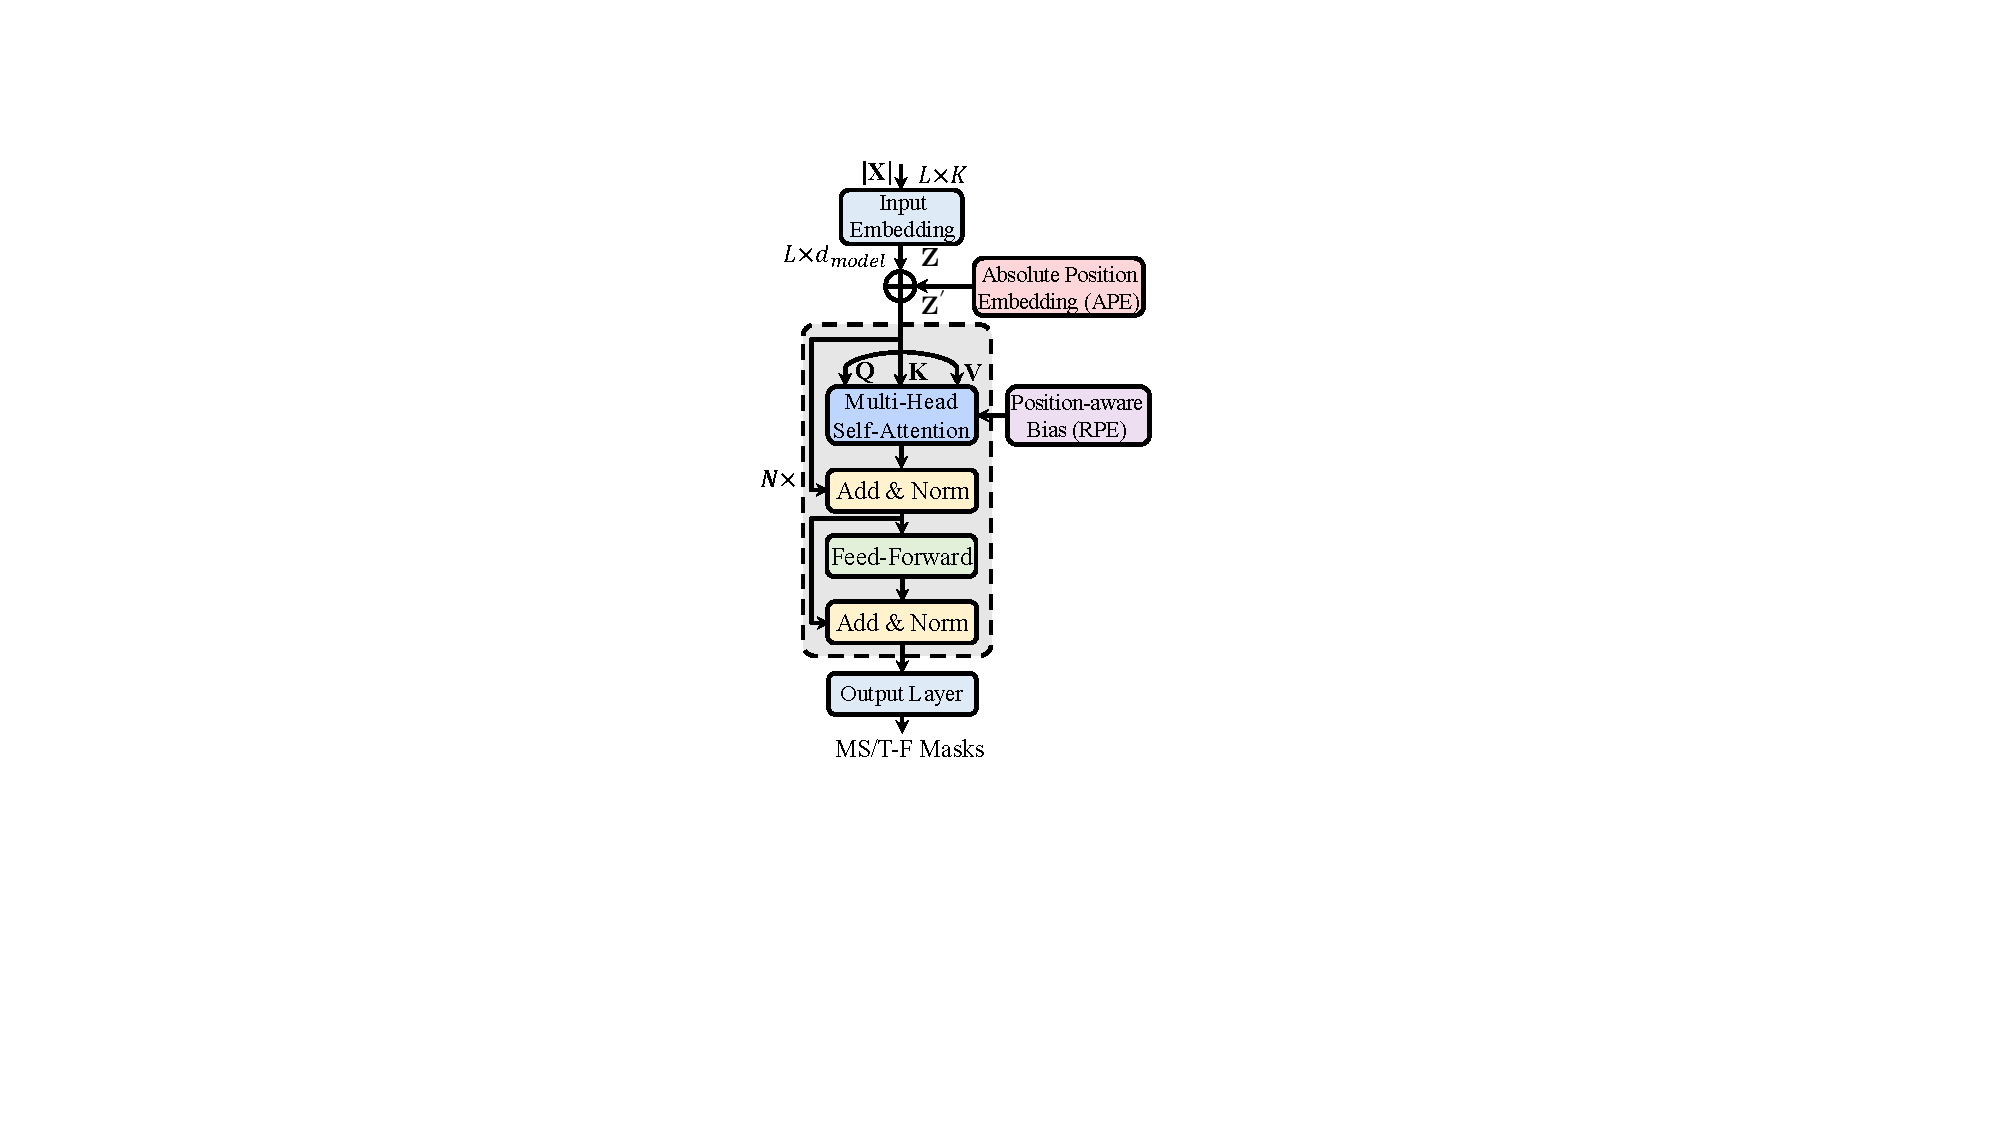
\includegraphics[width=0.99\columnwidth]{./diagram/Fig2a.pdf}}
\caption{}
\end{subfigure}
\hfill
\begin{subfigure}[t]{0.45\columnwidth}
\centerline{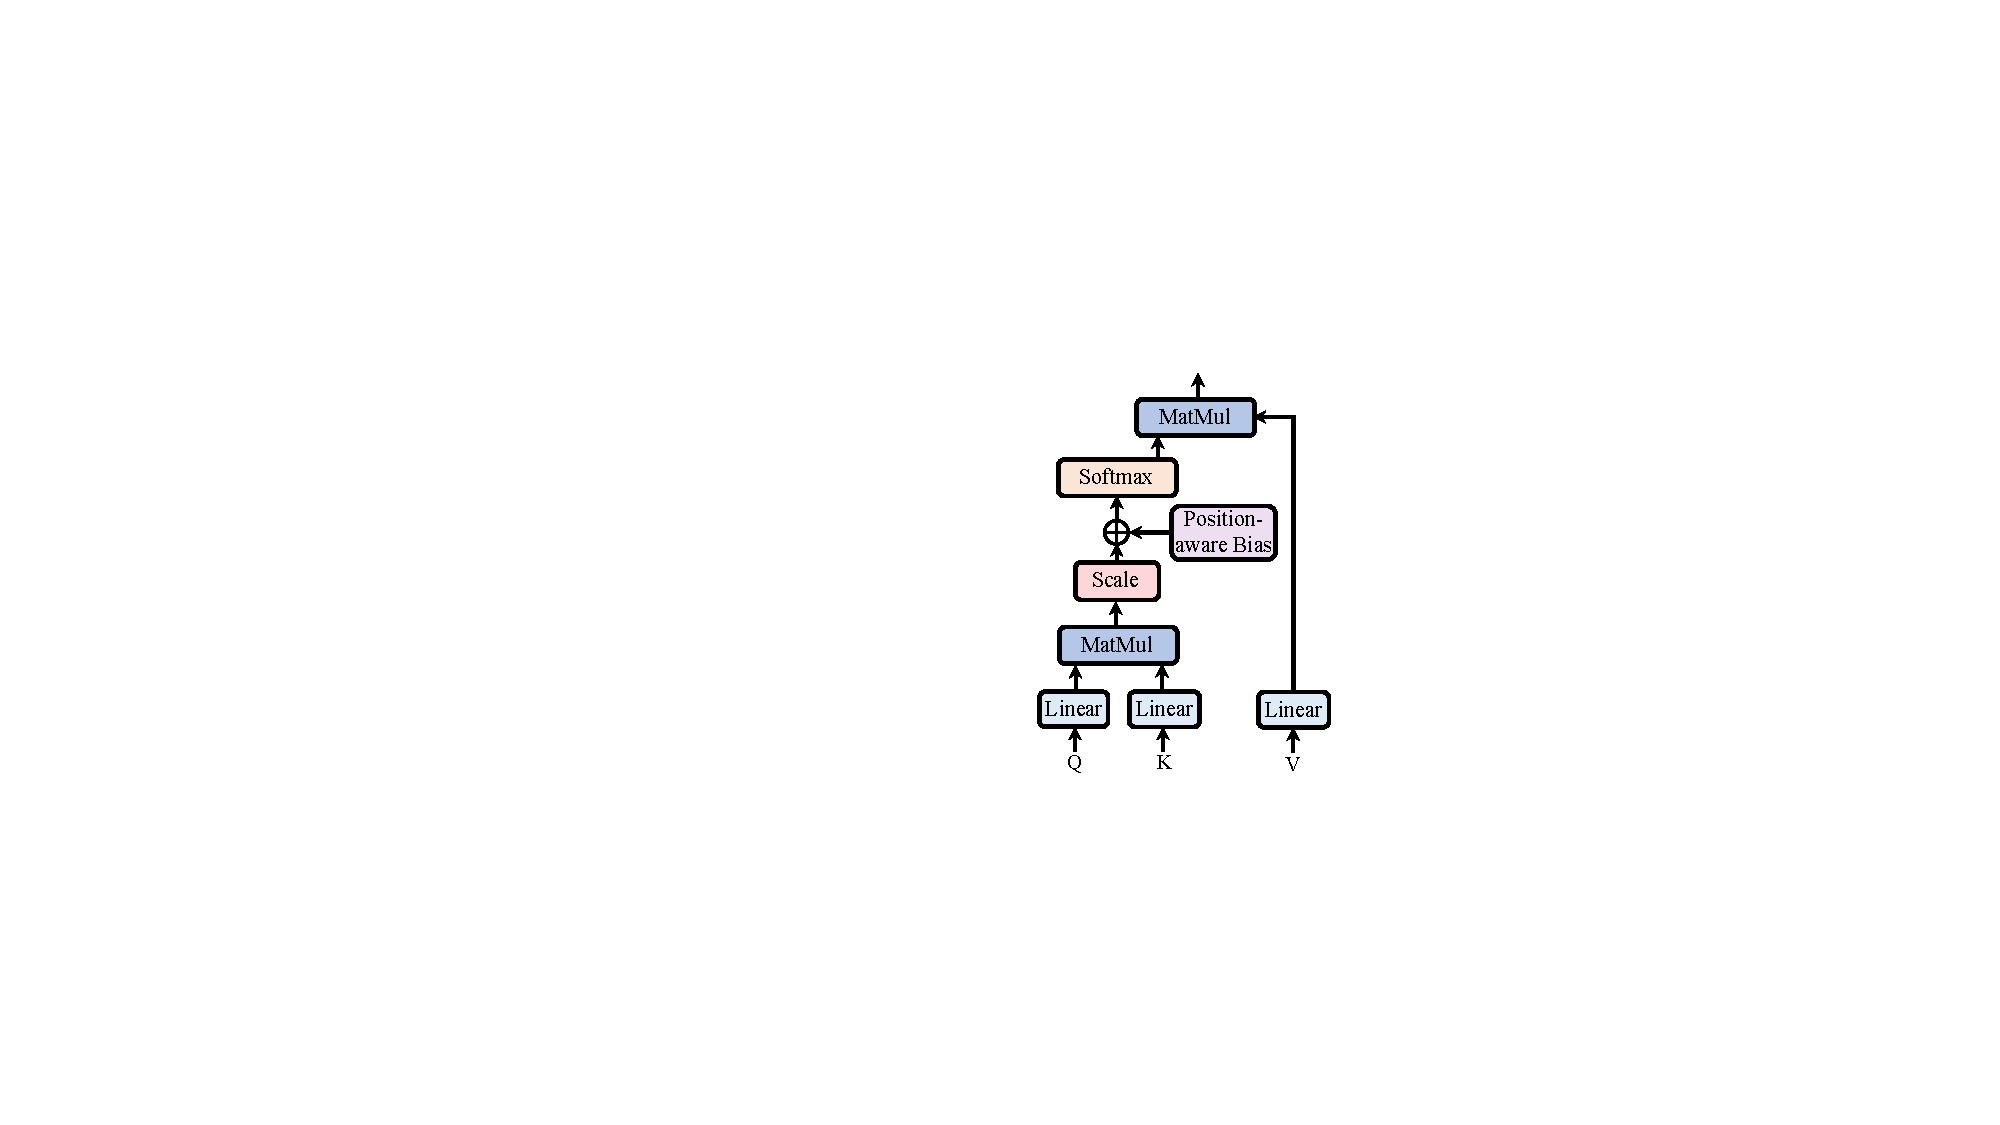
\includegraphics[width=0.99\columnwidth]{./diagram/Fig2b.pdf}}
\caption{}
\end{subfigure}
\caption{\textcolor{black}{Illustration of (a) the position-aware Transformer backbone network and (b) the position-aware self-attention. $\oplus$ denotes the element-wise summation operation.}}
\vspace{-1.8em}
\label{fig2}
\end{figure}

\begin{figure*}[!ht]
% \vskip -0.2in
\begin{center}
\centerline{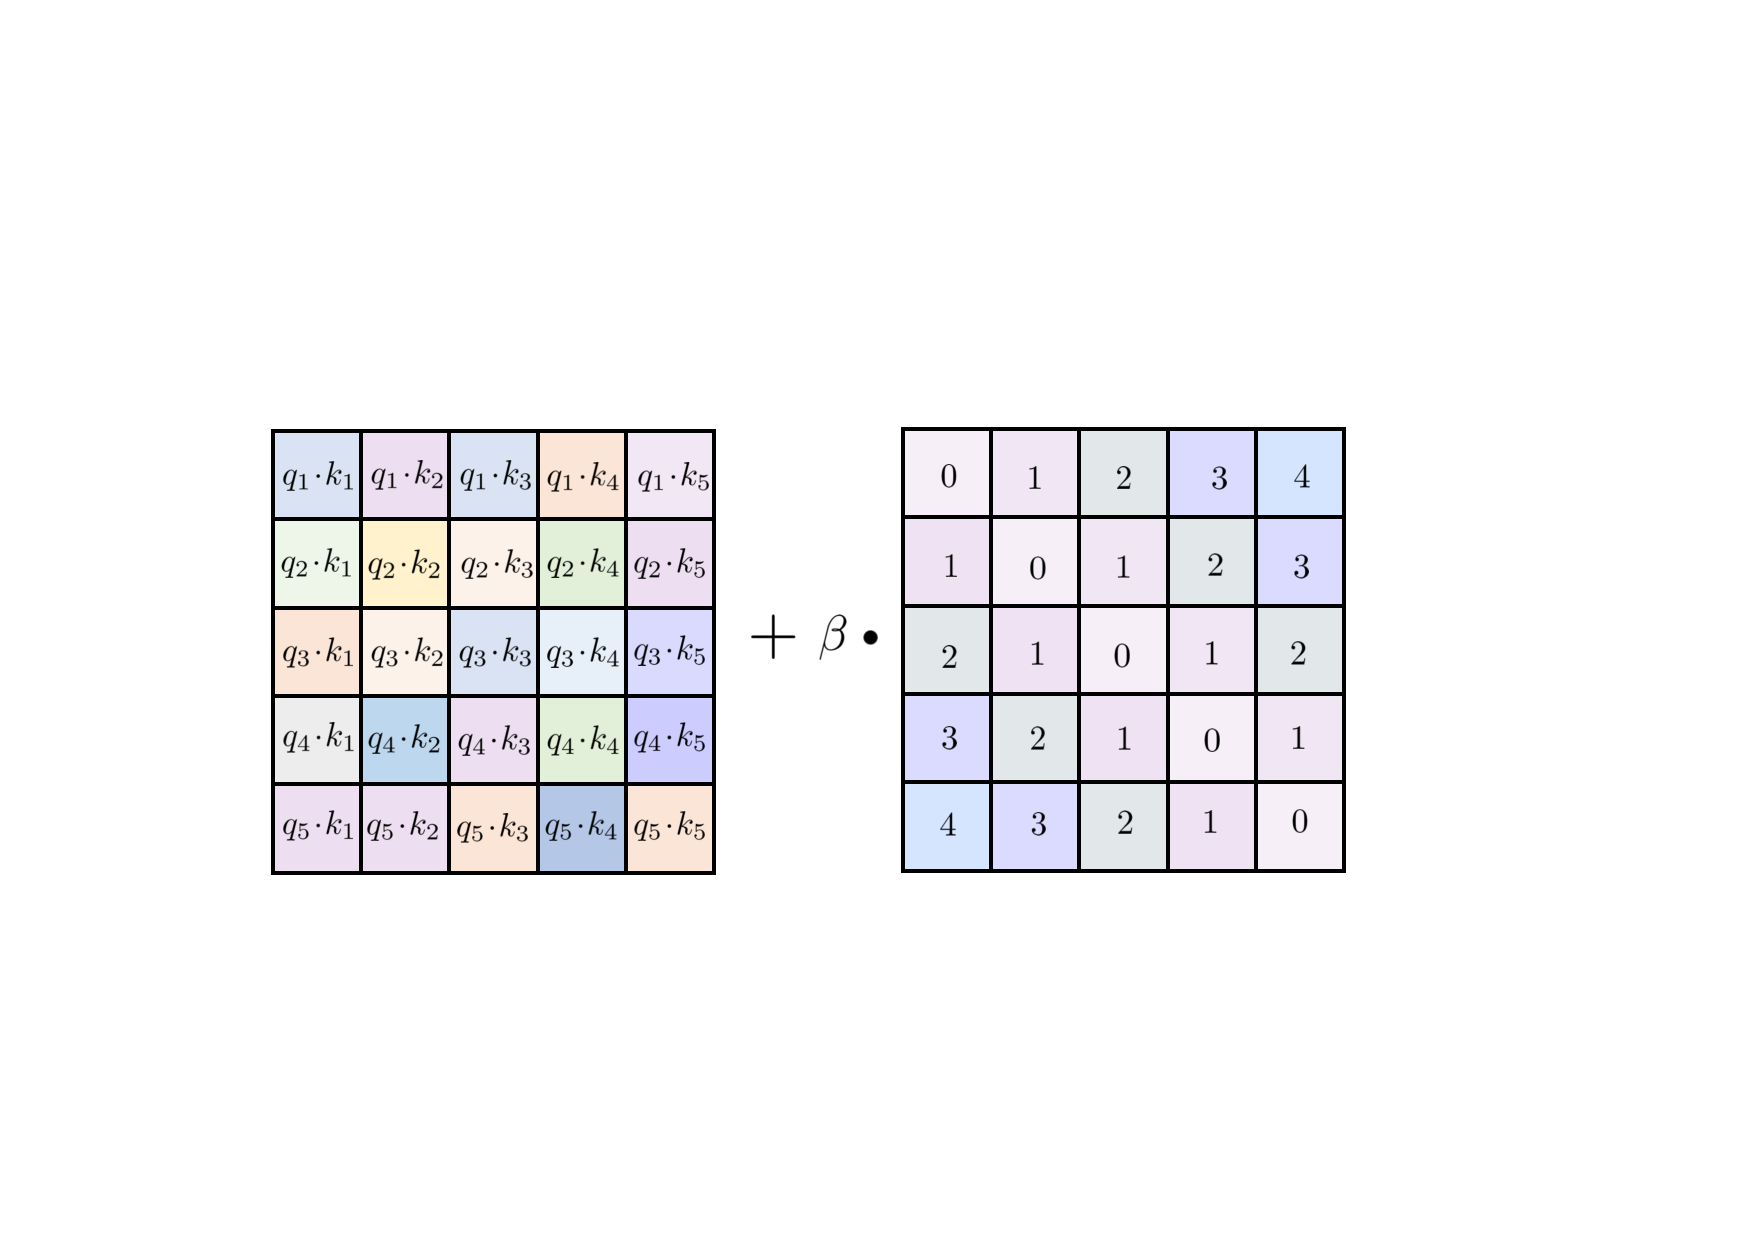
\includegraphics[width=1.39\columnwidth]{./diagram/Fig3.pdf}}
\caption{Raw dot-product attention scores are biased by adding a learnable position-aware bias. $\beta$ denotes the learnable head-wise scale parameter, which is different for each attention head shared across Transformer layers.}
\label{LearnLin}
\end{center}
% \vskip -0.2in
\vspace{-2.0em}
\end{figure*}

\subsection{\textcolor{black}{Position-aware Self-attention}}\label{sec4.2}

\textcolor{black}{Fig.~\ref{fig2} (b) illustrates the workflow of the position-aware self-attention module. It takes as input a set of queries ($\textbf{Q}\!\in \!\mathbb{R}^{L\times d_{model}}$), keys ($\textbf{K}\!\in\!\mathbb{R}^{L\times d_{model}}$), and values ($\textbf{V}\!\in\!\mathbb{R}^{L\times d_{model}}$), and a total of $H$ attention heads are utilized to allow the model to pay attention to different aspects of information, where we denote the head index as $h\!=\!\left\{1,2,3,..,H\right\}$.}

% \textcolor{black}{Each position-aware Transformer layer consists of two sub-layers. The first one is a multi-head self-attention (MHSA) module with a position-aware bias, and the second one is a two-layer fully connected feed-forward network (FFN). \textcolor{blue}{A residual skip connection~\cite{resnet} is employed around each sub-layer.} Fig. \ref{fig2} (b) illustrates the workflow of the position-aware self-attention module. It takes as input a set of queries ($\textbf{Q}\!\in \!\mathbb{R}^{L\times d_{model}}$), keys ($\textbf{K}\!\in\!\mathbb{R}^{L\times d_{model}}$), and values ($\textbf{V}\!\in\!\mathbb{R}^{L\times d_{model}}$), and a total of $H$ attention heads are utilized to allow the model to pay attention to different aspects of information, where we denote the head index as $h\!=\!\left\{1,2,3,..,H\right\}$.}


\textcolor{black}{For the $h$-th attention head, $\textbf{Q}$, $\textbf{K}$, and $\textbf{V}$ are first transformed with a linear projection respectively, which leads to $\textbf{Q}^{h}\!=\!\textbf{Q}\textbf{W}_{Q}^{h}$, $\textbf{K}^{h}\!=\!\textbf{K}\textbf{W}_{K}^{h}$, and $\textbf{V}^{h}\!=\!\textbf{V}\textbf{W}_{V}^{h}$, with dimensions of $d_{k}$, $d_{k}$, and $d_{v}$, respectively, where $\{\textbf{W}^{h}_{Q}, \textbf{W}_{K}^{h}\}\!\in\!\mathbb{R}^{d_{model}\times d_{k}}$ and $\textbf{W}_{V}^{h}\in\!\mathbb{R}^{d_{model}\times d_{v}}$ denote learned projection matrices. The scaled dot-product attention is used to compute the attention scores for each attention head. \textcolor{black}{This study explores \textcolor{black}{six} advanced RPE methods (described in Section~\ref{sec:3.2}) to enable the model to generalize from short speech utterances to longer ones. RoPE rotates query $\textbf{Q}$ and key $\textbf{K}$ representations with angles proportional to their absolute positions to incorporate position information in self-attention~\cite{RoPE}. DA-Bias injects position information by multiplying the clipped attention scores with the position-aware bias (refer to Equation (6) in~\cite{DA}).} In the other four RPE methods (Gauss-Bias, T5-Bias, TISA, and KERPLE), the position-aware bias or embeddings are injected with the element-wise summation operation before Softmax normalization, given as:}
\begin{equation}
    \textbf{A}^{h} \left(\textbf{Q}^{h}, \textbf{K}^{h}, \textbf{V}^{h}\right) = \text{softmax}\left(\frac{\textbf{Q}^{h}\textbf{K}^{h\top}}{\sqrt{d_{k}}}+\textbf{P}^{h}\right)\textbf{V}^{h},
\end{equation}
where $\top$ denotes the transpose operation, the head dimension $d_{k}\!=\!d_{v}\!=\!d_{model}/{H}$, and $\textbf{P}^{h}\!\in\!\mathbb{R}^{L\times L}$ the position-aware bias. We refer the reader to the original study \cite{attention2017} for more detailed descriptions of attention scores computation.

% This study explores \textcolor{blue}{six} advanced RPE methods (described in Section~\ref{sec:3.2}) to enable the model to generalize from short speech utterances to longer ones. \textcolor{blue}{Note that DA-Bias injects position information by multiplying the clipped attention scores with the position-aware bias (refer to Equation (6) in~\cite{DA}) and RoPE rotates $\textbf{Q}$ and $\textbf{K}$ with angles proportional to their absolute positions to incorporate position information in self-attention~\cite{RoPE}.}

Here, we also explore a simpler RPE scheme for length generalization. Similarly, $\textbf{P}^{h}$ is calculated by explicitly using the relative position between time frames. 
To be specific, let us denote the relative distance matrix as $\textbf{R}\!\in\!\mathbb{R}^{L\times L}$, where the $(i,j)$ entry $R_{i,j}\!=\!|i-j|$ denotes the real relative distance between the $i$-th and $j$-th time frames. We attempt to discard complex encoding designs (or formulations) in prior methods (TISA, KERPLE, and DA-Bias) \cite{tisa,kerple,DA} and use only one learnable parameter $\beta^{h}$ to scale $\textbf{R}$ in each attention head to compute the position-aware bias:
\begin{equation}
    P^{h}_{i,j} = \beta^{h} \cdot |i-j|.
\end{equation}
The head-wise scale parameter $\beta^{h}$ is shared across Transformer layers, with a different parameter for different attention heads. Hence, there are $H$ learnable parameters for $H$ attention heads. Unlike Gauss-Bias (Equation (\ref{gauss-bias})), ALiBi, and KERPLE (Equation (\ref{kerple})) that constrain the bias inversely proportional to $R_{i,j}\!=\!|i-j|$, we do not apply such a constraint to learn the position-aware bias. \textcolor{black}{A different parameter $\beta^{h}$ is learned in each attention head to enable different heads to model their diverse preferences on long-term or short-term contextual dependencies with different intensities, allowing the model to capture contextual dependencies more effectively. To be specific, a positive $\beta^{h}$ encourages the attention head to model long-term dependencies, as the attention scores are amplified more intensively by a more positive $P^{h}$. A negative $\beta^{h}$ encourages it to model short-term dependencies, as the attention scores are diminished more intensively by a more negative $P^{h}$.} Since the bias $P^{h}_{i,j}$ is learnable and linear to the real relative position, we refer to it as ``LearnLin''. We can also observe that LearnLin equals the term $w|i-j|$ in DA-Bias (Equation (\ref{dabias})). This study shows that the learnable sigmoidal function is redundant and leads to a performance decrease. Fig.~\ref{LearnLin} provides an example of how the LearnLin bias is injected into the self-attention mechanism (with a sequence length of $L=5$ time frames).

% The head-wise scale parameter $\beta^{h}$ is shared across Transformer layers, with different parameters for each attention head. Hence, there are $H$ learnable parameters for $H$ attention heads. Unlike Gauss-Bias (Equation (\ref{gauss-bias})), ALiBi, and KERPLE (Equation (\ref{kerple})) that constrain the bias inversely proportional to $R_{i,j}\!=\!|i-j|$, we do not make a such constraint to learn the position-aware bias. A positive $\beta^{h}$ encourages the attention head to model long-term dependencies, and a negative $\beta^{h}$ encourages it to model short-term dependencies. A different $\beta^{h}$ is learned for each head, which enables different heads to model contextual dependencies with different preferences. Since the bias $P^{h}_{i,j}$ is learnable and linear to the real relative position, we refer to it as ``LearnLin''. We can also observe that LearnLin equals the term $w|i-j|$ in DA-Bias (Equation (\ref{dabias})). This study shows that the learnable sigmoidal function is redundant and leads to a performance decrease. Fig.~\ref{LearnLin} provides an example of how the LearnLin bias is injected into the self-attention mechanism (with a sequence length of $L=5$ time frames).

% \textbf{Position Encoding}.

% \textcolor{black}{\textbf{Position Encoding}. \textcolor{blue}{In this study, we explore five strong RPE methods (described in Section \ref{sec:3.2}) to enable Transformer-based speech enhancement models to perform length generalization.}
% $\textbf{P}^{h}$ is calculated by explicitly using the relative position between time frames. To be specific, we denote the relative position matrix as $\textbf{R}\!\in\!\mathbb{R}^{L\times L}$, where the $(i,j)$ entry $R_{i,j}\!=\!|i-j|$ denotes the real relative position between the $i$-th and $j$-th time frames. A learnable parameter $\beta$ is applied to scale $\textbf{R}$ in each attention head to compute the position-aware bias:
% \begin{equation}
%     P^{h}_{i,j} = \beta^{h} \cdot |i-j|.
% \end{equation}
% The head-wise scale parameter $\beta^{h}$ is shared across Transformer layers, with different parameters for each attention head. Hence, there are $H$ learnable parameters for $H$ attention heads. Since the bias $P^{h}_{i,j}$ is learnable and linear to the real relative position, we refer to it as ``LearnLin''. Fig. \ref{LearnLin} provides an example of how the LearnLin bias is injected into the self-attention mechanism (with a sequence length of $L=5$ time frames).}

The outputs from all $H$ attention heads are then concatenated and transformed again with a linear projection $\textbf{W}^{O}\!\in\!\mathbb{R}^{d_{model}\times d_{model}}$, forming the MHSA module output:
\begin{equation}
    \text{MHSA}\left(\textbf{Q}, \textbf{K}, \textbf{V}\right) = \text{Concat}[\textbf{A}^{1}\!,\textbf{A}^{2}\!,...,\textbf{A}^{H}]\textbf{W}^{O}.
\end{equation}
The output of the MHSA sub-layer denoted by $\textbf{Y}$ is then passed to the two-layer FFN for two linear transformations, where a ReLU function is applied for the first layer, given as:
\begin{equation}
    \text{FFN}(\textbf{Y}) = \text{ReLU}(\textbf{Y}\textbf{W}_{1} + \textbf{b}_{1})\textbf{W}_{2} + \textbf{b}_{2},
\end{equation}
where $\textbf{W}_{1}\in \mathbb{R}^{d_{model}\times d_{f\!f}}$, $\textbf{W}_{2}\in \mathbb{R}^{d_{f\!f}\times d_{model}}$, $\textbf{b}_{1}\in \mathbb{R}^{d_{f\!f}}$, and $\textbf{b}_{2}\in \mathbb{R}^{d_{model}}$ are projection and bias parameters. The input and output of the FFN sub-layer have a dimension of $d_{model}$, and the dimension of the inner-layer is $d_{f\!f}$.

% \textcolor{blue}{\textbf{Discussion}:}


% {$d_{k}=d_{v} = d_{model}/{H}$, and $\textbf{K}_{h}^\top$ denotes the transpose of the $h$-th head of keys, $\textbf{K}_{h}$. An upper triangular mask is used to mask out the similarities that include future frames. For more detailed descriptions about attention function, we refer the reader to the original study \cite{attention2017}. The outputs of attention heads are concatenated and linearly projected again, yielding the output of the MHA module as:}


% \begin{equation}
%     \text{MHA}\left(\textbf{Q}, \textbf{K}, \textbf{V}\right) = \text{Concat}(\textbf{A}_{1},...,\textbf{A}_{H})\textbf{W}^{O},
% \end{equation}
% where $\textbf{W}^{O}\!\in\!\mathbb{R}^{d_{model}\times d_{model}}$. The TFA module takes the output from the previous MHA module, and conducts a T-F attention operation (described in Section \ref{sec3.1}) to tell the model to focus on the informative spectral components, resulting in an augmented T-F representation.



%\textcolor{red}{Dear Prof. Li, our two backbone ResTCN (TASLP 2020) and MHANet (Speech Communication 2020) are competitive. SOTA speaker separation model ConvTasNet are also based on ResTCN network. In introduction, we may already describe their success on speech enhancement (page 2, paragraph 2)? Here, we describe them and cite the corresponding references. In addition, we also compare ResTCN+TFA with ResTCN+SA baseline (TASLP 2020) in Table IV, which further confirms the efficiency and efficacy of TFA. As our paper focus on a module to improve existing models not developing a sota SE system, I did not report the comparison results with other sota models before. If it is necessary, we can provide more comparisons with other speech enhancement systems as in Table VIII of section IV-D. I will further describe the results if needed.}

% \textcolor{blue}{Our proposed \textcolor{blue}{TFA module} is applicable to general neural speech enhancement architecture. To set the stage for this study, in Figure \ref{fig1}, we illustrate a typical neural solution to speech enhancement, it is referred to as the backbone network in this paper. Here, two recently proposed backbone networks, \textcolor{blue}{ResTCN} \cite{DeepMMSE} and \textcolor{blue}{Transformer} \cite{mhanet,attention2017}, are employed. As the key component of the \textcolor{blue}{Transformer} layer \cite{attention2017} is the \textcolor{blue}{MHA} module, we term the \textcolor{blue}{Transformer} layer as a \textcolor{blue}{MHANet} block. The network takes the noisy spectral magnitude as input, $|\textbf{X}|\!\in\! \mathbb{R}^{L \times K}$, where $L$ and $K$ denote the number of time frames and frequency bins, respectively. The first layer consists of a 1-D convolution layer with a frame-wise layer normalization followed by the ReLU activation function, that encodes the input into a latent T-F representation of $\mathbb{R}^{L \times d_{model}}$. The output of the first layer is then fed into $B$ stacked ResTCN or MHANet blocks to perform T-F feature transformation. Following the last transformation block is the output layer, which is a 1-D convolution layer with a sigmoidal activation function that generates the estimates of IRM, SMM, PSM, and Xi.}

% \textcolor{blue}{We propose a \textcolor{blue}{TFA module} that is applicable to general neural speech enhancement architecture. To set the stage for this study, in Figure \ref{fig1}, we illustrate a typical neural solution to speech enhancement, it is referred to as the backbone network in this paper. Here, two recently proposed backbone networks, \textcolor{blue}{ResTCN} \cite{DeepMMSE} and \textcolor{blue}{Transformer} \cite{mhanet,attention2017}, are employed. As the key component of the \textcolor{blue}{Transformer} layer \cite{attention2017} is the \textcolor{blue}{MHA} module, we term the \textcolor{blue}{Transformer} layer as a \textcolor{blue}{MHANet} block. The network takes a noisy spectral magnitude as input, $|\textbf{X}|\!\in\! \mathbb{R}^{L \times K}$, where $L$ and $K$ denote the number of time frames and frequency bins, respectively. The first layer consists of a 1-D convolution layer with a frame-wise layer normalization followed by the ReLU activation function, that encodes the input into a latent T-F representation of $\mathbb{R}^{L \times d_{model}}$. The output of the first layer is then fed into $B$ stacked ResTCN or MHANet blocks to perform T-F feature transformation. Following the last transformation block is the output layer, which is a 1-D convolution layer with a sigmoidal activation function that generates the estimates of IRM, SMM, PSM, and Xi.} 

% \begin{figure}[!ht]
% % \vskip 0.1in
% \centering
% \begin{subfigure}[t]{0.52\columnwidth}
% \centerline{\includegraphics[width=0.93\columnwidth]{./diagram/resnet.pdf}}
% \caption{The original ResTCN block}
% \end{subfigure}\hfill
% \begin{subfigure}[t]{0.4\columnwidth}
% \centerline{\includegraphics[width=0.77\columnwidth]{./diagram/resnet_tfa.pdf}}
% \caption{The proposed ResTCN block with TFA module}
% \end{subfigure}
% \caption{Illustration of (a) the ResTCN block and (b) the ResTCN block with the proposed TFA module. $\bigoplus$ denotes the element-wise summation operation.}
% \label{ResTCN}
% \vspace{-1.0em}
% \end{figure}


% \subsubsection{\textcolor{blue}{TFA in ResTCN}}\label{resnet_model}

% \textcolor{blue}{In Figure \ref{ResTCN}, we illustrate a backbone network based on a \textcolor{blue}{ResTCN} block \cite{DeepMMSE} and  how the proposed TFA module works inside the \textcolor{blue}{ResTCN} block. As shown in Figure \ref{ResTCN}(a), the ResTCN block consists of three 1-D causal dilated convolutional modules. Each convolutional module employs a pre-activation design, where the input is pre-activated using frame-wise layer normalization followed by the ReLU activation function. We denote the kernel size, number of filters, and dilation rate for each convolutional module as a tuple of three elements. The first and third convolutional modules have a kernel size of 1, whilst the second convolutional module has a kernel size of $k$. The number of filters is $d_{f}$ for the first and second convolutional modules, and $d_{model}$ for the third convolutional module. The dilation rate, $d$, is employed in the second convolutional module, providing a contextual field over previous speech frames. The dilation rate is cycled as the block index $b\!=\!\left\{1,2,3,...,B\right\}$ increases: $d=2^{\left(b-1 \bmod \left(\log _{2}(D)+1\right)\right.}$, where mod is the modulo operation and $D\!=\!16$ is the maximum dilation rate.} 

% \textcolor{blue}{As shown in Figure \ref{ResTCN}(b), a \textcolor{blue}{TFA module} is augmented to the \textcolor{blue}{ResTCN} block to attend to the salient T-F representation. The residual connection \cite{resnet} is applied between the input and output of the block to facilitate gradient optimization.}


% \subsubsection{\textcolor{blue}{TFA in MHANet}}\label{mha_model}

% \textcolor{blue}{In Figure \ref{MHA}, we illustrate how a TFA module is incorporated into the MHANet backbone \cite{mhanet}. As shown in Figure \ref{MHA}(a), the MHANet block comprises two sub-blocks. The first is an MHA module, and the second is a two-layer fully connected feed-forward network (FFN). A residual connection is applied in each sub-block, followed by frame-wise layer normalization. To capture the T-F energy distribution of speech, as shown in Figure \ref{MHA}(b), we propose to incorporate a TFA module into the MHA module.} 
% The proposed \textcolor{blue}{MHANet} block with our \textcolor{blue}{TFA module} is described as follows.

% In the MHA module, a total of $H$ attention heads are employed to enable the model to pay attention to different aspects of information, where $h\!=\!\left\{1,2,3,...,H\right\}$ is the head index. 
% For $h$-th attention head, given an intermediate latent T-F tensor $\textbf{U}\!\in\!\mathbb{R}^{L\times d_{model}}$ as the input to the block, the MHA module first projects the input $\textbf{U}$ to queries ($\textbf{Q}_{h}\!\in \!\mathbb{R}^{L\times d_{k}}$), keys ($\textbf{K}_{h}\!\in\!\mathbb{R}^{L\times d_{k}}$), and values ($\textbf{V}_{h}\!\in\!\mathbb{R}^{L\times d_{v}}$):
% $\textbf{Q}_{h}\!=\!\textbf{U}\textbf{W}_{h}^{Q}$, $\textbf{K}_{h}\!=\!\textbf{U}\textbf{W}_{h}^{K}$, and $\textbf{V}_{h}\!=\!\textbf{U}\textbf{W}_{h}^{V}$, 
% where $\{\textbf{W}_{h}^{Q}, \textbf{W}_{h}^{K}\} \in \mathbb{R}^{d_{model}\times d_{k}}$, and $\textbf{W}_{h}^{V}\in \mathbb{R}^{d_{model}\times d_{v}}$ are different, learned linear projections. 
% The scaled dot-product attention is applied to each head in parallel, and the output is given as:
% \begin{equation}
%     \textbf{A}_{h} = \text{Attention}\left(\textbf{Q}_{h}, \textbf{K}_{h}, \textbf{V}_{h}\right) = \text{softmax}\left(\frac{\textbf{Q}_{h}\textbf{K}_{h}^\top}{\sqrt{d_{k}}}\right)\textbf{V}_{h},
% \end{equation}
% where $d_{k}=d_{v} = d_{model}/{H}$. An upper triangular mask is used to mask out the similarities that include future frames. For more detailed descriptions about attention function, we refer the reader to the original study \cite{attention2017}. The outputs for each attention head are concatenated and linearly projected again, yielding the output of the MHA module as:
% \begin{equation}
%     \text{MHA}\left(\textbf{U}\right) = \text{Concat}(\textbf{A}_{1},...,\textbf{A}_{H})\textbf{W}^{O},
% \end{equation}
% where $\textbf{W}^{O}\!\in\!\mathbb{R}^{d_{model}\times d_{model}}$. The TFA module takes the output from the previous MHA module, and conducts a T-F attention operation (described in Section \ref{sec3.1}) to tell the model to focus on the informative spectral components, resulting in an augmented T-F representation. 

% \textcolor{blue}{Given an intermediate latent T-F tensor $\textbf{U}\!\in\!\mathbb{R}^{L\times d_{model}}$ as the input to the block, the MHA module first projects the input $\textbf{U}$ to queries ($\textbf{Q}\!\in \!\mathbb{R}^{L\times d_{model}}$), keys ($\textbf{K}\!\in\!\mathbb{R}^{L\times d_{model}}$), and values ($\textbf{V}\!\in\!\mathbb{R}^{L\times d_{model}}$):
% $\textbf{Q}\!=\!\textbf{U}\textbf{W}^{Q}$, $\textbf{K}\!=\!\textbf{U}\textbf{W}^{K}$, and $\textbf{V}\!=\!\textbf{U}\textbf{W}^{V}$, where 
% $\left\{\textbf{W}^{Q}, \textbf{W}^{K}, \textbf{W}^{V}\right\}\in \mathbb{R}^{d_{model}\times d_{model}}$ are different, learned linear projections. Then they are split into $H$ attention heads, indexed by $h=\left\{1,2,3,...,H\right\}$, and with dimensions $d_{k}$, $d_{k}$, and $d_{v}$, respectively, which enables the model to pay attention to different aspects of information. The scaled dot-product attention is applied to each head in parallel to generate the output,
% \begin{equation}
%     \textbf{A}_{h} = \text{Attention}\left(\textbf{Q}_{h}, \textbf{K}_{h}, \textbf{V}_{h}\right) = \text{softmax}\left(\frac{\textbf{Q}_{h}\textbf{K}_{h}^\top}{\sqrt{d_{k}}}\right)\textbf{V}_{h},
% \end{equation}
% where $d_{k}=d_{v} = d_{model}/{H}$, and $\textbf{K}_{h}^\top$ denotes the transpose of the $h$-th head of keys, $\textbf{K}_{h}$. An upper triangular mask is used to mask out the similarities that include future frames. For more detailed descriptions about attention function, we refer the reader to the original study \cite{attention2017}. The outputs for each attention head are concatenated and linearly projected again, yielding the output of the MHA module as:
% \begin{equation}
%     \text{MHA}\left(\textbf{Q}, \textbf{K}, \textbf{V}\right) = \text{Concat}(\textbf{A}_{1},...,\textbf{A}_{H})\textbf{W}^{O},
% \end{equation}
% where $\textbf{W}^{O}\!\in\!\mathbb{R}^{d_{model}\times d_{model}}$. The TFA module takes the output from the previous MHA module, and conducts a T-F attention operation (described in Section \ref{sec3.1}) to tell the model to focus on the informative spectral components, resulting in an augmented T-F representation.}


% \textcolor{blue}{The two-layer FFN takes the output $\textbf{U}^{'}\!\in\! \mathbb{R}^{L\times d_{model}}$ from the first sub-block, and performs two linear transformations with a ReLU activation in the first layer:
% \begin{equation}
%     \text{FFN}(\textbf{U}^{'}) = \text{max}(0, \textbf{U}^{'}\textbf{W}^{1} + \textbf{b}^{1})\textbf{W}^{2} + \textbf{b}^{2},
% \end{equation}
% where $\textbf{W}^{1}\in \mathbb{R}^{d_{model}\times d_{f\!f}}$, $\textbf{b}^{1}\in \mathbb{R}^{d_{f\!f}}$, $\textbf{W}^{2}\in \mathbb{R}^{d_{f\!f}\times d_{model}}$, and $\textbf{b}^{2}\in \mathbb{R}^{d_{model}}$. The size of input and output is $d_{model}$, and the inner-layer has a size of $d_{f\!f}$.}

% \textbf{{Model Configuration.}}
% For ResTCN backbone, we adopt the parameter settings as in \cite{DeepMMSE} to build the network: $d_{model}\!=\!256$, $B\!=\!40$, $d_{f}\!=\!64$, and $k\!=\!3$.
% For MHANet backbone, we follow the parameter settings in \cite{mhanet}: $B\!=\!5$, $d_{model}\!=\!256$, $H\!=\!8$, and $d_{f\!f}\!=\!1024$. For our proposed TFA module, a kernel size $k_{t\!f\!a}\!=\!17$ is adopted in the dilated 1-D convolution.


%\textcolor{red}{we need to justify why we use two 1D map to form a 2D map? why not directly estimate a 2D map?} \\
%\textcolor{red}{There are multiple ways to compute a 2D attention map. the most straightforward method is to apply a 2D attention directly. because time-frequency bins are correlated, when we compute 1D along time axis and 1D along freq axis, basically we ignore the time-frequency relationship which is against our own idea. }

%\textcolor{red}{This paper is written like a technical report, there is no justification nor substantiation. we simply say we do this, we do that. this is not the way to write a scientific paper. for example, we say that 1-D attention first uses a global average pooling, ... who proved this is the best, and there is not alternative? is it because there is no other way to do the same thing, or because it is already proven by a reference (cite the paper) that this works better than other alternative? for example, why don't we do a 2D attention map directly? we cannot simply exclude other options in the theoretical explanation. this section is for us to debate what is the best solution, and is NOT for us to tell what we do. only after we debate what is the best, then we can zoom into a solution. otherwise, the paper is seen as a technical report, simply reporting what we have done. Readers are not interested in what we do at all, 99\% of readers/reviewers learn how we motivate our idea and algorithms, and use our ideas in their work. No one will repeat our experiments unless they agree that the method is absolutely the best way to the problem, and it is our job to prove that we offer the best way.  ---- please justify why neural speech enhancement solution needs a TFA module in Section II.C!n i don't see anything in introduction that justify the need of a TFA module in neural speech enhancement architecture. please point to me which line? in the introduction, we only say the T-F attention is not used, but there is no justification that TFA like the one we propose may lead to an improvement.}
%\textcolor{blue}{Thank you Prof. Li. I have revised the description in this section.}

% \subsection{Implementation}\label{sec3.2}
% The proposed time-frequency attention is applicable to neural speech enhancement architecture in general. Here we integrate it into two widely used backbones, i.e., ResTCN and Transformer. As the MHA module is the  key component of the Transformer layer, we term the Transformer layer as a MHANet block. 


% In this subsection, we will give detailed descriptions of the architecture configuration of models. All models employ the architecture as shown in figure \ref{architecture}. The input is the noisy spectral magnitude, $|\textbf{X}|\in \mathbb{R}^{L \times K}$, where $L$ and $K$ denote the number of time frames and frequency bins, respectively. The first layer projects the input to an embedding with a size of $d_{model}$, where a fully-connected layer that includes frame-wise layer normalization followed by the ReLU activation function is employed. The output of the first layer is then fed into $B$ stacked transformation blocks (shown in Figure \ref{ResTCN} and \ref{MHA}). Following the last block is the output layer, which is a fully-connected layer with a sigmoidal activation function. 

% \begin{figure}[!ht]
% % \vskip 0.2in
% \begin{center}
% \centerline{\includegraphics[width=0.4\columnwidth]{diagram/framework.pdf}}
% \caption{Architecture of models.}
% \label{architecture}
% \end{center}
% \vskip -0.2in
% \end{figure}


\section{Experimental Setup}\label{sec:6}

\subsection{Dataset}\label{sec:4.1}
\textcolor{black}{In this section, we provide a detailed description of the clean speech and noise data used in our experiments. For the clean speech data in the training set, we employ the \textit{train-clean-100} subset of the LibriSpeech corpus \cite{Librispeech}, comprising $28\,539$ clean speech utterances from $251$ speakers ($125$ females and $126$ males), with a total duration of approximately 100 hours. The noise data used for training are collected from the Nonspeech dataset \cite{Nonspeech}, the RSG-10 dataset \cite{RSG}, the Environmental Background Noise dataset \cite{ENV1,ENV2}, the Urban Sound dataset \cite{Urban}, the noise subset of the MUSAN corpus \cite{MUSAN}, the QUT-NOISE dataset \cite{QUT}, and the colored noise data (with an $\alpha$ value ranging from $-2$ to $2$ in increments of 0.25) \cite{DeepMMSE}. For testing, we select four noise sources \cite{tfaj}: \textit{factory welding}, \textit{F16}, and \textit{voice babble} from the RSG-10 dataset \cite{RSG} and the \textit{street music} recording no $26\,270$ from the Urban Sound dataset \cite{Urban}. The noise recordings in the dataset that are longer than 30 seconds are split into clips of 30 seconds or less, resulting in a noise set with a total of $6\,809$ noise clips. To perform validation experiments, we randomly selected $1\,000$ clean speech utterances (over 2 seconds) and noise clips from the clean speech and noise data to create a validation set of $1\,000$ noisy speech utterances. The noisy utterances are synthesized by mixing each clean speech with a random segment of one noise clip at a random SNR sampled from the set $\left\{r|r\in \mathbb{Z}: -10 \leq r \leq 20 \right\}$ (dB). As a result, the training set includes a total of $27\,539$ clean speech utterances and $5\,809$ noise clips.}

For evaluation experiments, clean speech utterances are taken from the \textit{test-clean-100} subset of LibriSpeech corpus \cite{Librispeech}. Noise clips are from the aforementioned four real-world noise recordings drawn from the RSG-10 noise dataset \cite{RSG} and the Urban Sound dataset \cite{Urban}, containing two colored (\textit{factory welding} and \textit{F16}) and two non-stationary noise sources (\textit{street music} and \textit{voice babble}).

\begin{figure}[!t]
% \vskip 0.1in
\centering
\centerline{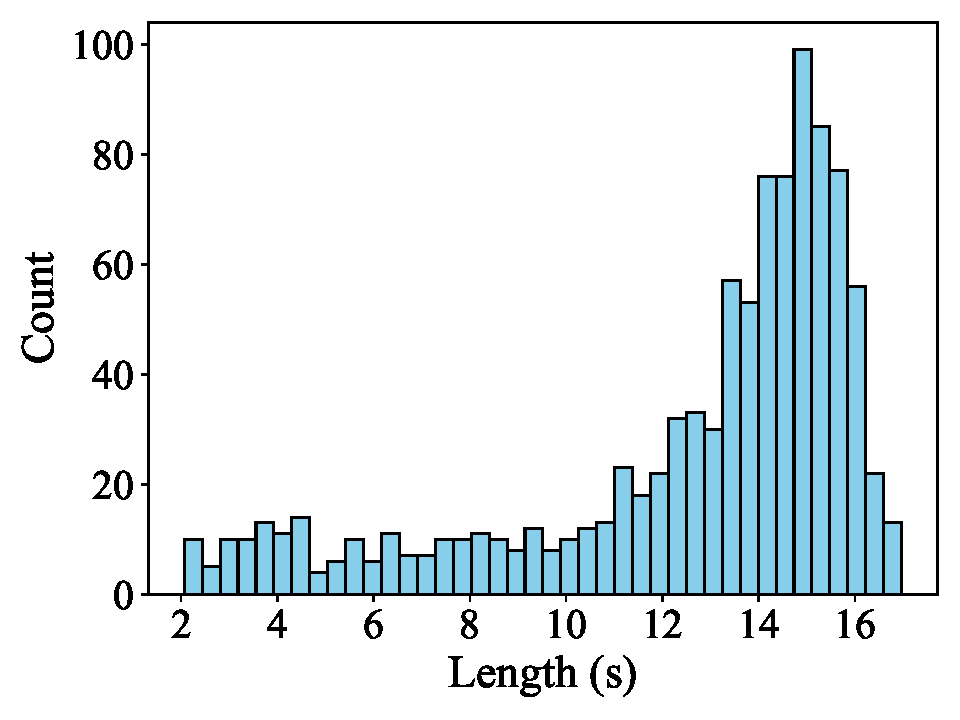
\includegraphics[width=0.82\columnwidth]{./diagram/Fig4.pdf}}
\caption{The length distribution over the $1000$ speech utterances in the validation dataset.}
\label{val_length}
\vspace{-1.5em}
\end{figure}

\textbf{Feature Extraction.} \textcolor{black}{All audio signals used in this study are monaural and sampled at a rate of 16 kHz. The noisy speech utterance is segmented into a set of time frames using a square-root-Hann window of length 32 ms ($32\!\times\!16\!=\!512$ time samples), with a hop length of 16 ms ($16\!\times\!16\!=\!256$ time samples). A 512-point fast Fourier transform (FFT) is then applied to each frame, resulting in a 257-dimensional STFT magnitude spectrum as the input, which contains both the DC and Nyquist frequency components.}


\textbf{Length Generalization}. To investigate the length generalization performance of the models, clean speech utterances in the training set are split into 1-second (1s) and 2-second (2s) speech clips for training, respectively. The training details are described in Section \ref{sec:4.2}. For testing, we create six test sets, of which each consists of 400 noisy speech recordings of 1s, 2s, 5s, 10s, 15s, and 20s in length, respectively. The noisy mixtures are generated as follows: we randomly select twenty clean speech utterances (over 1s, 2s, 5s, 10s, 15s, and 20s in length, respectively) from the \textit{test-clean-100} subset for each of the four test noise recordings. Then, a random clip (1s, 2s, 5s, 10s, 15s, and 20s in length) from each clean speech utterance is corrupted by a random clip with the same length cut from the noise recording at five SNR levels, i.e., -5 dB, 0 dB, 5 dB, 10 dB, and 15 dB. In Fig. \ref{val_length}, we provide the distribution of lengths over the $1\ 000$ speech utterances in the aforementioned validation set. We can find that the validation lengths show a broad range (diversity) and most of the speech utterances are more than four times (4s or 8s) the length of the training set (1s or 2s).
% which demonstrates the effectiveness of the validation set in length generalization experiments.

% Ten clean speech utterances (without replacement) are randomly drawn from the \textit{test-clean-100} subset for each of the four noise recordings, and each clean speech is corrupted by a random clip cut from the noise recordings at five SNRs, i.e., -5 dB, 0 dB, 5 dB, 10 dB, and 15 dB. It forms $200$ noisy mixtures for evaluation.

% \subsection{Feature Extraction} \label{sec:4.0}
% \textcolor{black}{All audio signals used in our experiment are with a sampling rate of 16 kHz. For spectral analysis, a square-root-Hann analysis window of length 32 ms (512 time samples) is adopted to segment noisy speech into time frames with 50\% overlapping (256 time samples). Each time frame is transformed using a 512-point fast Fourier transform (FFT) operation, leading to a 257-point single-sided STFT magnitude spectrum of noisy speech as the input to networks.}


% (excluded from the noise set) 
% aforementioned 
% we adopt the recordings of four real-world noise sources (excluded from training set) including two non-stationary and two coloured. The two non-stationary noise sources are the \textit{voice babble} from the RSG-10 noise dataset \cite{RSG} and \textit{street music} from the Urban Sound dataset \cite{Urban}. The two coloured noise sources are \textit{F16} and \textit{factory welding} from RSG-10 noise dataset \cite{RSG}. For each of the four noise recordings, ten clean speech recordings (without replacement) randomly selected from the \textit{test-clean-100} of Librispeech corpus \cite{Librispeech} are mixed with a random segment of the noise recordings at the following SNR levels: $\left\{ -5 \text{ dB}, 0 \text{ dB}, 5 \text{ dB}, 10 \text{ dB}, 15 \text{ dB} \right\}$. This generates $200$ noisy mixtures for evaluation.

% sampled from -10 to 20 dB.
% $\left\{s|s\in \mathbb{Z}: -10 \leq s \leq 20 \right\}$ (dB).

% For clean speech recordings, we use the \textit{train-clean-100} set from the Librispeech corpus \cite{Librispeech} as the training set, which includes $28\,539$ utterances spoken by $251$ speakers. The noise recordings in the training set are taken from the following datasets: the QUT-NOISE dataset \cite{QUT}, the Nonspeech dataset \cite{Nonspeech}, the Environmental Background Noise dataset \cite{ENV1,ENV2}, the RSG-10 dataset \cite{RSG} (\textit{voice babble}, \textit{F16}, and \textit{factory welding} are excluded for testing), the Urban Sound dataset \cite{Urban} (\textit{street music} recording no $26\,270$ is excluded for testing), the noise set from the MUSAN corpus \cite{MUSAN}, and coloured noise recordings (with an $\alpha$ value ranging from $-2$ to $2$ in increments of 0.25). Noise recordings that are over 30 seconds in length are split into segments of $30$ seconds or less. This gives a total of $6\,809$ noise recordings, each with a length less than or equal to $30$ seconds. For validation experiments, we randomly select $1\,000$ clean speech and noise recordings (without replacement) and remove them from the aforementioned clean speech and noise sets. Each clean speech recording is mixed with a random section of one noise recording at a randomly selected SNR level between $-10$ dB and $20$ dB in 1 dB increments. This generates $1\,000$ noisy speech signals as the validation set.

% Let us first describe the clean speech and noise data in this study. For clean speech recordings, we use the \textit{train-clean-100} set from the Librispeech corpus \cite{Librispeech} as the training set, which includes $28\,539$ utterances spoken by $251$ speakers. The noise recordings in the training set are taken from the following datasets: the QUT-NOISE dataset \cite{QUT}, the Nonspeech dataset \cite{Nonspeech}, the Environmental Background Noise dataset \cite{ENV1,ENV2}, the RSG-10 dataset \cite{RSG} (\textit{voice babble}, \textit{F16}, and \textit{factory welding} are excluded for testing), the Urban Sound dataset \cite{Urban} (\textit{street music} recording no $26\,270$ is excluded for testing), the noise set from the MUSAN corpus \cite{MUSAN}, and coloured noise recordings (with an $\alpha$ value ranging from $-2$ to $2$ in increments of 0.25). Noise recordings that are over 30 seconds in length are split into segments of $30$ seconds or less. This gives a total of $6\,809$ noise recordings, each with a length less than or equal to $30$ seconds. For validation experiments, we randomly select $1\,000$ clean speech and noise recordings (without replacement) and remove them from the aforementioned clean speech and noise sets. Each clean speech recording is mixed with a random section of one noise recording at a randomly selected SNR level between $-10$ dB and $20$ dB in 1 dB increments. This generates $1\,000$ noisy speech signals as the validation set. 

% For evaluation experiments, we adopt the recordings of four real-world noise sources (excluded from training set) including two non-stationary and two coloured. The two non-stationary noise sources are the \textit{voice babble} from the RSG-10 noise dataset \cite{RSG} and \textit{street music} from the Urban Sound dataset \cite{Urban}. The two coloured noise sources are \textit{F16} and \textit{factory welding} from RSG-10 noise dataset \cite{RSG}. For each of the four noise recordings, ten clean speech recordings (without replacement) randomly selected from the \textit{test-clean-100} of Librispeech corpus \cite{Librispeech} are mixed with a random segment of the noise recordings at the following SNR levels: $\left\{ -5 \text{ dB}, 0 \text{ dB}, 5 \text{ dB}, 10 \text{ dB}, 15 \text{ dB} \right\}$. This generates $200$ noisy mixtures for evaluation.

% This section details the training methodology for training the models.

% \subsection{Training Methodology}


\subsection{Implementation Details}\label{sec:4.2}
In this section, we describe the details of model implementations. To evaluate the length generalization of the LearnLin, we employ the standard Transformer backbone network without position embedding (No-Pos) as the baseline \cite{mhanet}. The Transformer model employs $N\!=\!4$ Transformer layers \cite{ripple} and adopt the parameter settings as in \cite{tfaj}: $H\!=\!8$, $d_{model}\!=\!256$, and $d_{f\!f}\!=\!1024$. This study explores several existing APE and RPE methods, which include Sinusoidal \cite{attention2017}, BERT-Pos \cite{bert}, Gauss-Bias \cite{gaussbias}, T5-Bias \cite{T5}, TIAS \cite{tisa}, DA-Bias \cite{DA}, and KERPLE \cite{kerple}, to enable the Transformer speech enhancement model to perform length generalization. For TISA, the number of kernels $S$ is set to 5 \cite{tisa}. It should be noted that KERPLE is initially proposed for causal language modeling. In this study, we derive a non-causal version of KERPLE to study length generalization. Table \ref{params} lists the numbers of trainable parameters for different positional encoding methods. 



% Bicubic interpolation is applied to BERT-Pos for length generalization at validation and inference time.

\textcolor{black}{\textbf{Training Methodology}. Every ten clean speech utterances are selected from the training set and split into clean speech clips of length 1s and 2s (the last clip is dropped), respectively, to create one mini-batch for one training iteration. The noisy mixtures are generated on fly during training. Specifically, each clean speech clip from the mini-batch is corrupted by a random segment of a random noise clip with a randomly sampled SNR from $\left\{r|r\in \mathbb{Z}: -10 \leq r \leq 20 \right\}$ (dB). For each training epoch, the order of picking up clean speech is shuffled randomly. 
For all of the training objectives (i.e., MS, IRM, PSM, \textcolor{black}{and cIRM}), the mean-square error (MSE) is used as the training objective function. Mask approximation is used to learn the T-F mask. For MS, the MSE loss is computed on the power-law compressed magnitude spectrum \cite{2021interactive}. For optimization of the models, we adopt the Adam gradient optimizer with the hyper-parameter settings \cite{attention2017}, $\beta_{1}\!=\!0.9$, $\beta_{2}\!=\!0.98$, and $\epsilon\!=\!1\times10^{-9}$. The gradient clipping is applied to keep the gradient values in the range from -1 to 1. Since the gradient optimization of the self-attention based Transformer models requires a carefully designed learning rate scheduler, a warm-up scheduler is used to dynamically adjust the learning rate \cite{mhanet,attention2017}. Specifically, the formula used to adjust the learning rate is given as \cite{tfaj}:
\begin{equation}
\vspace{-0.2em}
    lr = d_{model}^{-0.5}\cdot \textrm{min} \left(n\_step \cdot w\_steps^{-1.5}, n\_step^{-0.5}\right)
\end{equation}
where $w\_steps$ and $n\_step$ denote the number of warm-up training steps and training steps, respectively. Following~\cite{mhanet}, we use $w\_steps\!=\!40\,000$ for warm-up training scheduler. Our experiments were conducted on an NVIDIA Tesla P100-PCIe-16GB graphics processing unit (GPU).}

% Within one mini-batch, all utterances are zero padded to the same length as the longest one.

%\subsection{Feature Extraction}
%All audio signals are monaural and sampled at 16 kHz. The noisy speech utterance is segmented into a set of time frames using a square-root-Hann window of length 32 ms ($32\!\times\!16\!=\!512$ time samples), with a hop length of 16 ms ($256$ time samples). A 512-point fast Fourier transform (FFT) operation is applied to each frame, leading to a 257-dimensional STFT magnitude spectrum as the input that contains both the DC and the Nyquist frequency components. \textcolor{red}{(to Qiquan: this subsection should be moved to Dataset subsection)} \\
%\textcolor{blue}{To Prof. Li: I have moved this paragraph (highlighted with blue color) to the Dataset section.}

\subsection{Assessment Metrics}
\textcolor{black}{Five commonly used objective assessment metrics, which are the perceptual evaluation of speech quality (PESQ) \cite{PESQ}, the extended short-time objective intelligibility (ESTOI) \cite{estoi}, and three composite metrics \cite{composite}, are adopted to comprehensively evaluate enhanced speech signals. Reading all the five speech assessment metrics, we have a higher score to indicate better performance. The PESQ and ESTOI are to evaluate the quality and intelligibility of enhanced speech, respectively. The PESQ score is in the range of $-0.5$ to $4.5$, and the ESTOI score typically ranges from 0 to 1. The three composite metrics describe the mean opinion score (MOS) of the overall speech quality (COVL) \cite{composite}, the signal distortion (CSIG) \cite{composite}, and the background-noise distortion (CBAK) \cite{composite}, respectively. The COVL, CSIG, and CBAK scores range from 0 to 5.}

\begin{table}[!t]
\centering
    \scriptsize
    % \def\arraystretch{1.3}
    % \setlength{\tabcolsep}{1.5pt}
    \def\arraystretch{1.3}
    \setlength{\tabcolsep}{1.3pt}
    \setlength{\abovetopsep}{0pt}
    \setlength\belowbottomsep{0pt} 
    \setlength\aboverulesep{0pt} 
    \setlength\belowrulesep{0pt}
\caption{The number of trainable parameters for different positional encoding methods, where $L^{'}$ and $S$ (set to 5 as suggested in \cite{tisa}) denote the fixed maximum length (frame numbers) and the kernel numbers in TISA.}
% \vspace*{-0.05in}
\scalebox{0.97}{\begin{tabular}{l|c|c|c|c|c|c|c|c }
\toprule[1.25pt]
% \hline
PE & Sinu. & BERT-Pos & Gauss-Bias & TISA & T5-Bias & DA-Bias & KERPLE & LearnLin \\
\hline
\textbf{\#Param.} & -- & $L^{'}\!\cdot\!d_{model}$ & $H$ & $3SHN$ & $32H$ & $2H$ & $2H$ & $H$ \\
% \hline
\toprule[1.25pt]
\end{tabular}}
\vspace{-1.5em}
\label{params}
\end{table}

% \textcolor{blue}{All the models are trained from scratch. For ResTCN \cite{DeepMMSE} and its TFA augmented variants, the \textit{Adam} algorithm with default hyper-parameters \cite{Adam} and a learning rate of $1\times10^{-3}$ is used for gradient descent optimisation. For MHANet \cite{mhanet} and its TFA augmented variant, the \textit{Adam} algorithm with parameters as in \cite{attention2017}, i.e., $\beta_{1}=0.9$, $\beta_{2}=0.98$, and $\epsilon\!=\!1\times10^{-9}$ is used for training. The gradient clipping technique is used for all models, where the gradients are clipped between -1 and 1. As the training of MHANet is sensitive to the learning rate \cite{mhanet,attention2017}, we adopt the warm-up training strategy in \cite{attention2017}, where the learning rate is adjusted during the training process according to the rule:
% \begin{equation}
% \vspace{-0.2em}
%     lr = d_{model}^{-0.5}\cdot \textrm{min} \left(n\_step^{-0.5}, n\_step \cdot w\_steps^{-1.5}\right)
% \end{equation}
% where $n\_step$ and $w\_steps$ denote the number of training steps and warm-up training steps, respectively. Following \cite{mhanet}, the number of steps $w\_steps\!=\!40\,000$ is adopted for warm-up training in this work.}

% \subsection{Training Methodology}
% Here, we describe the details of training methodology used in this study. A mini-batch size of $10$ noisy speech utterances is used for each training iteration. The noisy speech signals are created as follows: each clean speech recording selected for the mini-batch is mixed with a random section of a randomly selected noise recording at a randomly selected SNR level (-10 dB to 20 dB, in 1 dB increments). The selection order for the clean speech recordings is randomised for each epoch. For the three masking-based training objectives (i.e., IRM, SMM, and PSM), we adopt mask approximation to learn the mask, where the mean-square error (MSE) is the loss function. For Xi, the cross-entropy is employed as the loss function \cite{nicolson2019deep,DeepMMSE}. Each utterance in a mini-batch is padded with zeros, giving it the same number of time frames as the longest noisy utterance. 

% All the models are trained from scratch. For ResTCN \cite{DeepMMSE} and its TFA augmented variants, the \textit{Adam} algorithm with default hyper-parameters \cite{Adam} and a learning rate of $0.001$ is used for gradient descent optimisation. For MHANet \cite{mhanet} and its TFA augmented variant, the \textit{Adam} algorithm with parameters as in \cite{attention2017}, i.e., $\beta_{1}\!=\!0.9$, $\beta_{2}\!=\!0.98$, and $\epsilon\!=\!10^{-9}$ is used for training. The gradient clipping technique is used for all models, where the gradients are clipped between $[-1,1]$. As the training of MHANet is sensitive to the learning rate \cite{mhanet,attention2017}, we adopt the warm-up training strategy in \cite{attention2017}, where the learning rate is adjusted during the training process according to the rule:
% \begin{equation}
% \vspace{-0.2em}
%     lr = d_{model}^{-0.5}\cdot \textrm{min} \left(n\_step^{-0.5}, n\_step \cdot w\_steps^{-1.5}\right)
% \end{equation}
% where $n\_step$ and $w\_steps$ denote the number of training steps and warm-up training steps, respectively. Following \cite{mhanet}, the number of steps $w\_steps\!=\!40\,000$ is adopted for warm-up training in this work.

% \subsection{Evaluation Metrics}
% In our experiments, five widely used metrics are adopted for extensive speech enhancement evaluations, including perceptual evaluation of speech quality (PESQ) \cite{PESQ}, extended short-time objective intelligibility (ESTOI) \cite{estoi}, and three composite metrics \cite{composite}. For PESQ metric, we adopt the wide-band PESQ \cite{PESQ}, which typically produces a lower score than the narrow-band counterpart \cite{restcnsa}. The value range of PESQ is $[-0.5, 4.5]$ and the value of ESTOI is typically in $[0, 1]$. The three composite metrics are mean opinion score (MOS) predictors of the signal distortion (CSIG) \cite{composite}, the background-noise intrusiveness (CBAK) \cite{composite}, and the overall signal quality (COVL) \cite{composite}, respectively. The value range of the three composite metrics is $[0, 5]$. For all of the above five metrics, a higher score indicates better enhancement performance. The word error rate (WER\%) is adopted to evaluate the downstream ASR performance, and a lower WER\% score means better speech recognition performance.


% \subsection{Comparative Models}
% We evaluate the proposed TFA module as part of two backbone networks (ResTCN \cite{DeepMMSE} and MHANet \cite{mhanet}) on four training objectives. The proposed ResTCN and MHANet with the TFA module are denoted by ``ResTCN+TFA'' and ``MHANet+TFA'', respectively. In addition, we conduct an ablation study to validate the efficacy of each component (the TA and FA) in the TFA module. Similarly, we denote the ResTCN and MHANet with the TA and FA by ``ResTCN+TA'', ``MHANet+TA'',  ``ResTCN+FA'',  and ``MHANet+FA'', respectively. All models in this study are implemented using Tensorflow 1.13. \textcolor{blue}{Our experiments were conducted on an NVIDIA Tesla P100 graphics processing unit (GPU) and an Intel Xeon E5-2682 v4 CPU at 2.50 GHz (54 logical processors).}




% \begin{figure}[!htbp]
% % \vskip 0.1in
% \centering
% \begin{subfigure}[t]{0.495\columnwidth}
% \captionsetup{justification=centering}
% \centerline{\includegraphics[width=\columnwidth]{./loss_curves/mha_irm_train_symbol.pdf}}
% \caption{}
% \end{subfigure}\hfill
% \begin{subfigure}[t]{0.490\columnwidth}
% \centerline{\includegraphics[width=\columnwidth]{./loss_curves/mha_irm_val_symbol.pdf}}
% \caption{}
% \end{subfigure}
% \caption{The (a) training error and (b) validation error of MHANet and proposed models with MHANet as backbone on IRM training objective.}
% \vskip -0.2in
% \label{mha_irm}
% \end{figure}

% \begin{figure}[!h]
% % \vskip 0.1in
% \centering
% \begin{subfigure}[t]{0.495\columnwidth}
% \captionsetup{justification=centering}
% \centerline{\includegraphics[width=\columnwidth]{./loss_curves/resnet_train_smm_symbol.pdf}}
% \caption{}
% \end{subfigure}\hfill
% \begin{subfigure}[t]{0.495\columnwidth}
% \centerline{\includegraphics[width=\columnwidth]{./loss_curves/resnet_val_smm_symbol.pdf}}
% \caption{}
% \end{subfigure}
% \caption{The (a) training error and (b) validation error of ResTCN and proposed models with ResTCN as backbone on SMM training objective.}
% \vskip -0.2in
% \label{resnet_smm}
% \end{figure}

% \begin{figure}[!h]
% % \vskip 0.1in
% \centering
% \begin{subfigure}[t]{0.495\columnwidth}
% \captionsetup{justification=centering}
% \centerline{\includegraphics[width=\columnwidth]{./loss_curves/mha_train_smm_symbol.pdf}}
% \caption{}
% \end{subfigure}\hfill
% \begin{subfigure}[t]{0.495\columnwidth}
% \centerline{\includegraphics[width=\columnwidth]{./loss_curves/mha_val_smm_symbol.pdf}}
% \caption{}
% \end{subfigure}
% \caption{The (a) training error and (b) validation error of MHANet and proposed models with MHANet as backbone on SMM training objective.}
% \vskip -0.2in
% \label{mha_smm}
% \end{figure}

% \begin{figure}[!h]
% % \vskip 0.1in
% \centering
% \begin{subfigure}[t]{0.495\columnwidth}
% \captionsetup{justification=centering}
% \centerline{\includegraphics[width=\columnwidth]{./loss_curves/resnet_psm_train_symbol.pdf}}
% \caption{}
% \end{subfigure}\hfill
% \begin{subfigure}[t]{0.495\columnwidth}
% \centerline{\includegraphics[width=\columnwidth]{./loss_curves/resnet_psm_val_symbol.pdf}}
% \caption{}
% \end{subfigure}
% \caption{The training error (a) and validation error (b) of ResTCN and proposed models with ResTCN as backbone on PSM training objective.}
% \vskip -0.2in
% \label{resnet_psm}
% \end{figure}

% \begin{figure}[!h]
% % \vskip 0.1in
% \centering
% \begin{subfigure}[t]{0.495\columnwidth}
% \captionsetup{justification=centering}
% \centerline{\includegraphics[width=\columnwidth]{./loss_curves/mha_psm_train_symbol.pdf}}
% \caption{}
% \end{subfigure}\hfill
% \begin{subfigure}[t]{0.495\columnwidth}
% \centerline{\includegraphics[width=\columnwidth]{./loss_curves/mha_psm_val_symbol.pdf}}
% \caption{}
% \end{subfigure}
% \caption{The training error (a) and validation error (b) of MHANet and proposed models with MHANet as backbone on PSM training objective.}
% \vskip -0.2in
% \label{mha_psm}
% \end{figure}

% \begin{figure}[!ht]
% % \vskip 0.1in
% \centering
% \begin{subfigure}[t]{0.495\columnwidth}
% \captionsetup{justification=centering}
% \centerline{\includegraphics[width=\columnwidth]{./loss_curves/resnet_magXi_train_symbol.pdf}}
% \caption{}
% \end{subfigure}\hfill
% \begin{subfigure}[t]{0.495\columnwidth}
% \centerline{\includegraphics[width=\columnwidth]{./loss_curves/resnet_magXi_val_symbol.pdf}}
% \caption{}
% \end{subfigure}
% \caption{The training error (a) and validation error (b) of ResTCN and proposed models with ResTCN as backbone on Xi training objective.}
% \vskip -0.2in
% \label{resnet_magXi}
% \end{figure}

% \begin{figure}[!ht]
% % \vskip 0.1in
% \centering
% \begin{subfigure}[t]{0.495\columnwidth}
% \captionsetup{justification=centering}
% \centerline{\includegraphics[width=\columnwidth]{./loss_curves/mha_magXi_train_symbol.pdf}}
% \caption{}
% \end{subfigure}\hfill
% \begin{subfigure}[t]{0.495\columnwidth}
% \centerline{\includegraphics[width=\columnwidth]{./loss_curves/mha_magXi_val_symbol.pdf}}
% \caption{}
% \end{subfigure}
% \caption{The training error (a) and validation error (b) of MHANet and proposed models with MHANet as backbone on Xi training objective.}
% \vskip -0.3in
% \label{mha_magXi}
% \end{figure}

\begin{figure}[!b]
% \vskip -0.15in
\centering
\begin{subfigure}[t]{0.5\columnwidth}
\captionsetup{justification=centering}
\centerline{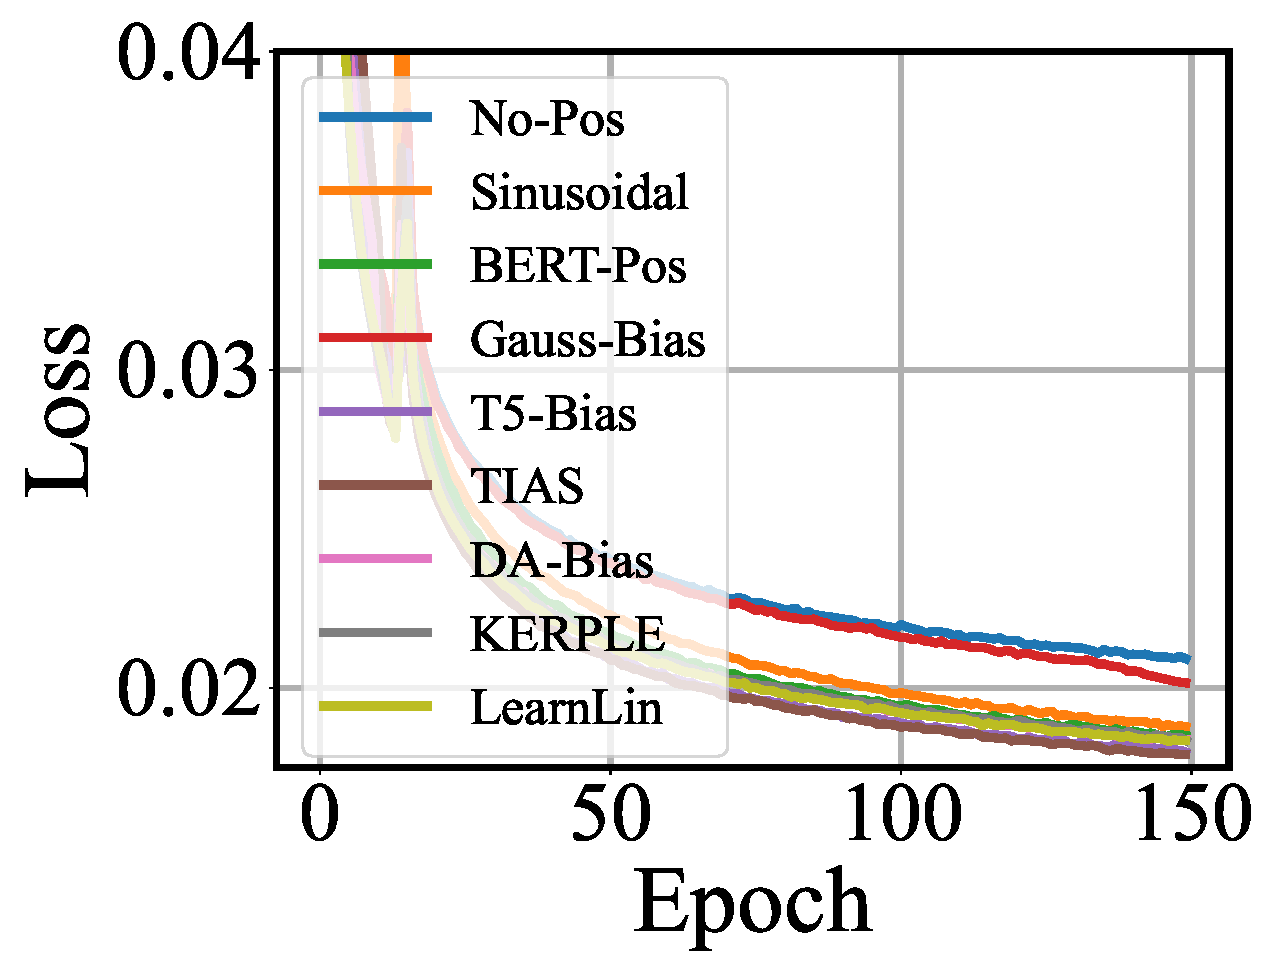
\includegraphics[width=\columnwidth]{./loss_curves/Fig5a.pdf}}
\caption{}
\end{subfigure}\hfill
\begin{subfigure}[t]{0.5\columnwidth}
\centerline{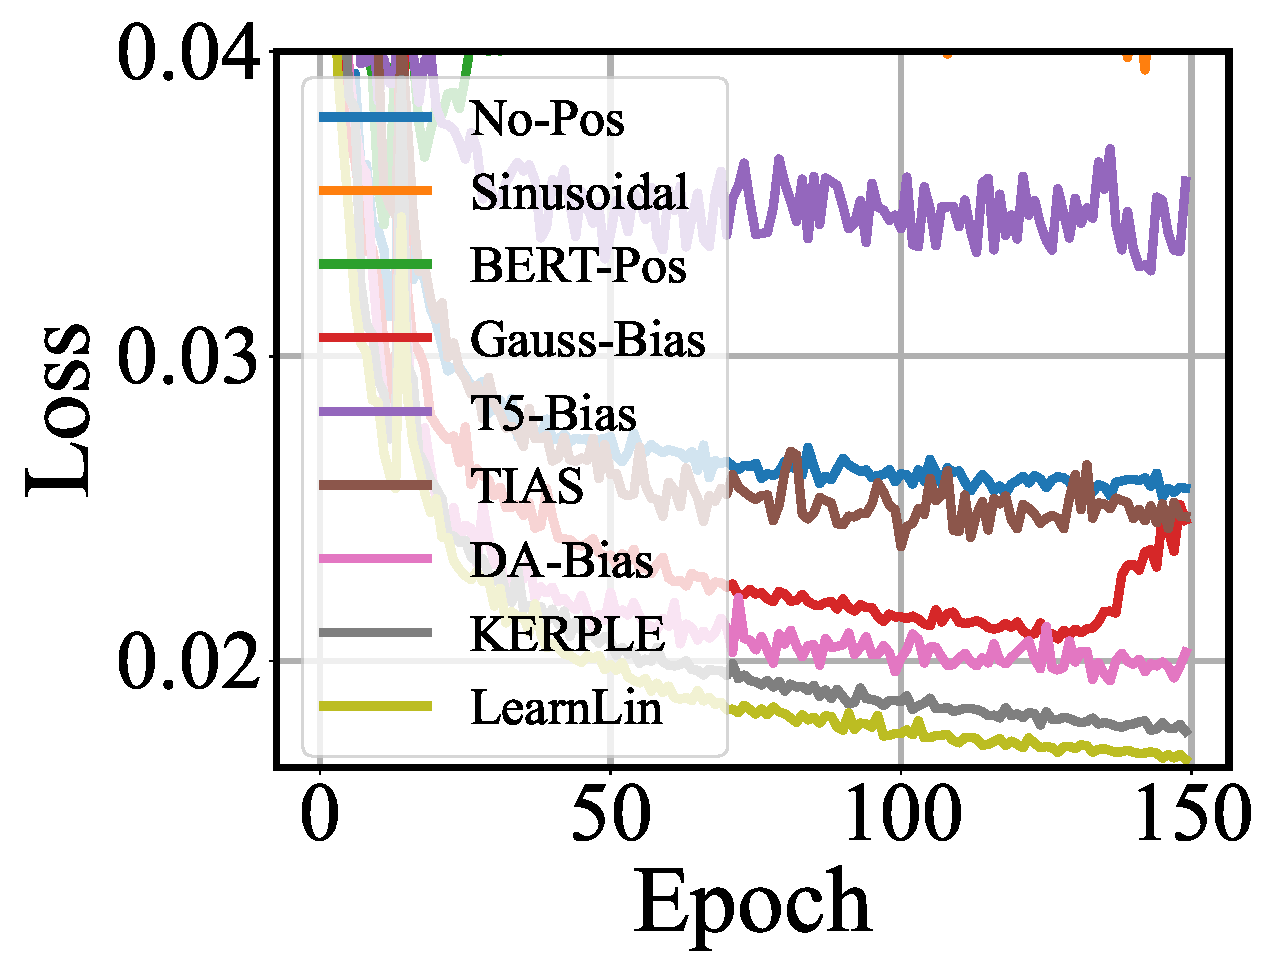
\includegraphics[width=\columnwidth]{./loss_curves/Fig5b.pdf}}
\caption{}
\end{subfigure}
\caption{The (a) training loss and (b) validation loss of the models trained using 1s utterances, on MS training objective. }
\vskip -1.0em
\label{train1s_MagMag}
\end{figure}
\section{Experimental Results}\label{sec:7}
% \subsection{Training and Validation Error}
% We first observe the training and validation errors across the models. The error curves produced by each of the models on the four training objectives (i.e., IRM, SMM, PSM, and Xi) are shown in Figures \ref{resnet_irm}-\ref{mha_irm}, Figures \ref{resnet_smm}-\ref{mha_smm}, Figures \ref{resnet_psm}-\ref{mha_psm}, and Figures \ref{resnet_magXi}-\ref{mha_magXi}, respectively, where each model is trained for 250 epochs. We observe similar trends of error curves on different training objectives. The purple curves are for ResTCN and MHANet, and the red curves are for ResTCN+TFA and MHANet+TFA. It can be easily observed that ResTCN+TFA and MHANet+TFA yield significantly lower training and validation errors than ResTCN and MHANet, which demonstrates the effect of the TFA module. In addition, the ablation study also confirms the efficacy of the FA and TA modules. One can observe that ResTCN+FA (blue curves) and ResTCN+TA (yellow curves) produce significantly lower training and validation error as compared to ResTCN. ResTCN+FA yields close error curves with ResTCN+TA. MHANet+FA (blue curves) and MHANet+TA (yellow curves) also achieve an obviously lower training and validation error than MHANet. For MHANet, applying the TA module achieves lower training and validation error than the FA module. Among the TFA, TA, and FA modules, the TFA module consistently produces the lowest training and validation error across different training objectives.
% \input{pesq.tex}
% \input{stoi.tex}

% \begin{figure}[!t]
% % \vskip -0.1in
% \centering
% \begin{subfigure}[t]{0.5\columnwidth}
% \captionsetup{justification=centering}
% \centerline{\includegraphics[width=\columnwidth]{./loss_curves_nokerple/MagSMM_Train1S_train.pdf}}
% \caption{}
% \end{subfigure}\hfill
% \begin{subfigure}[t]{0.5\columnwidth}
% \centerline{\includegraphics[width=\columnwidth]{./loss_curves_nokerple/MagSMM_Train1S_val.pdf}}
% \caption{}
% \end{subfigure}
% \caption{The (a) training loss and (b) validation loss of the models trained using 1s utterances, on SMM training objective. }
% \vskip -0.2em
% \label{train1s_MagSMM}
% \end{figure}


\begin{figure}[!t]
\vskip -0.1in
\centering
\begin{subfigure}[t]{0.5\columnwidth}
\captionsetup{justification=centering}
\centerline{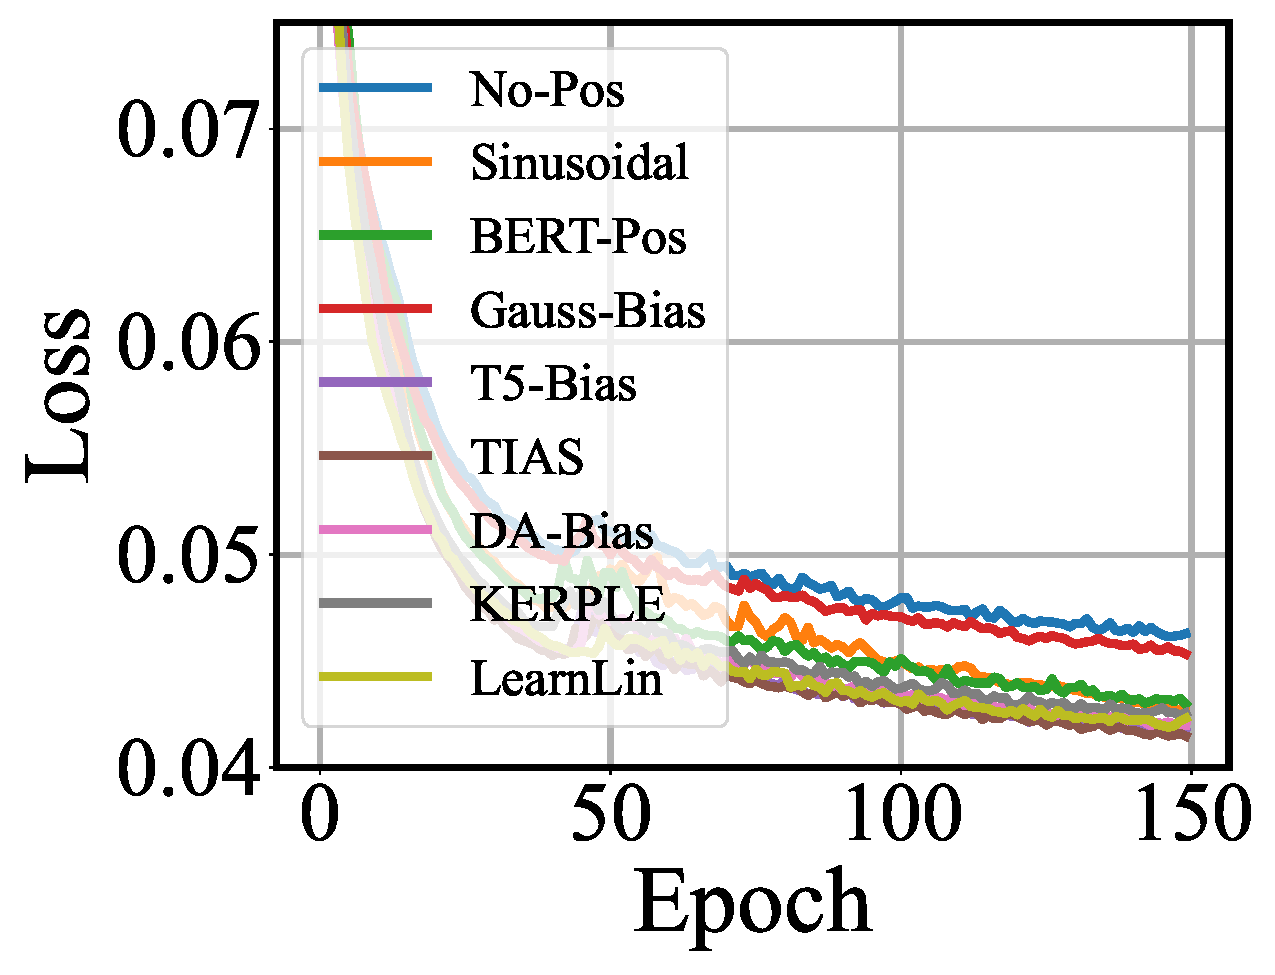
\includegraphics[width=\columnwidth]{./loss_curves/Fig6a.pdf}}
\caption{}
\end{subfigure}\hfill
\begin{subfigure}[t]{0.5\columnwidth}
\centerline{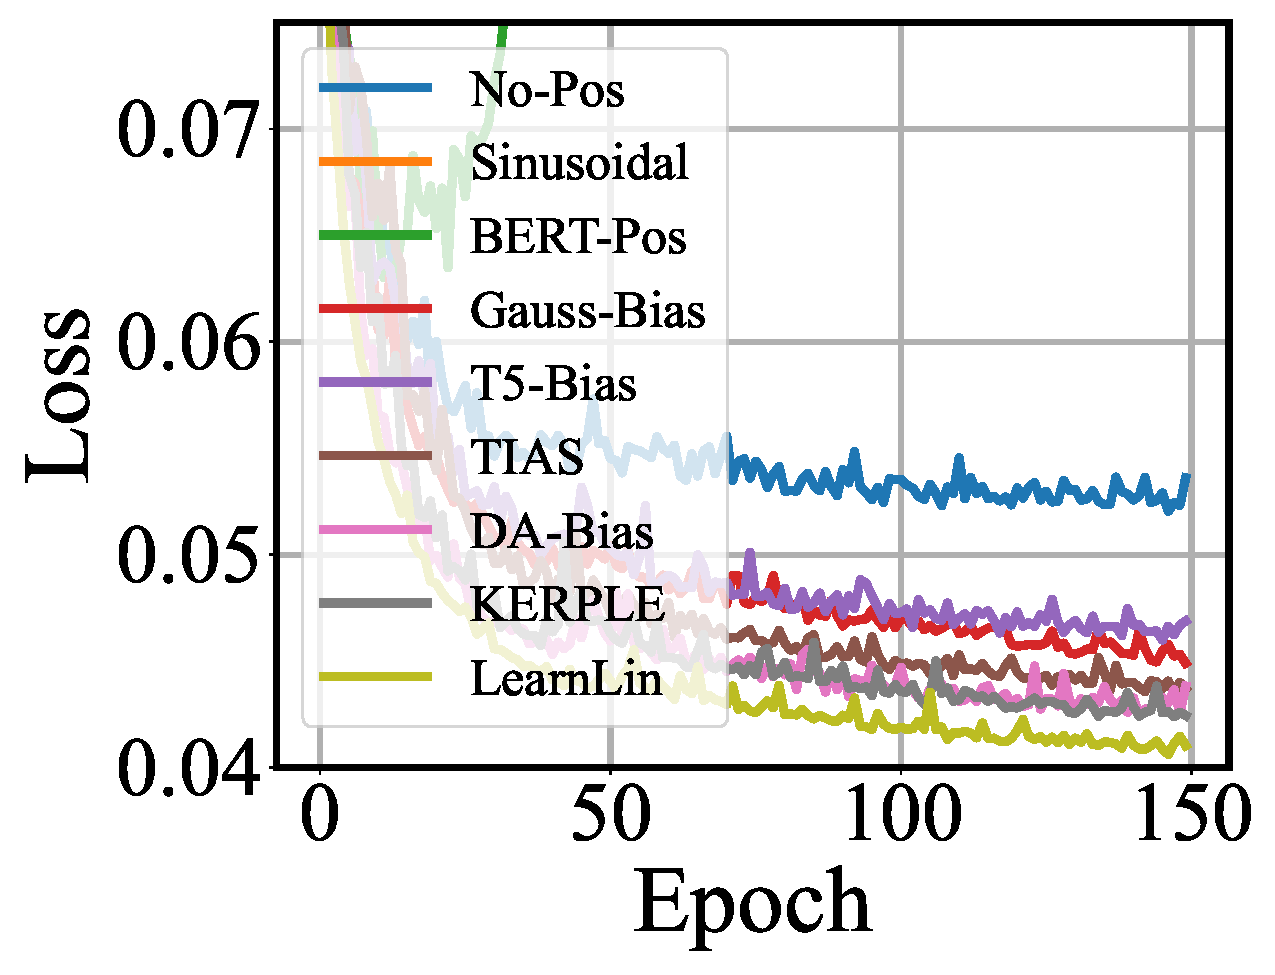
\includegraphics[width=\columnwidth]{./loss_curves/Fig6b.pdf}}
\caption{}
\end{subfigure}
\caption{The (a) training loss and (b) validation loss of the models trained using 2s utterances, on IRM training objective. }
\vspace{-0.2em}
\label{train2s_MagIRM}
\end{figure}

\begin{figure}[!t]
% \vskip -0.1in
\centering
\begin{subfigure}[t]{0.5\columnwidth}
\captionsetup{justification=centering}
\centerline{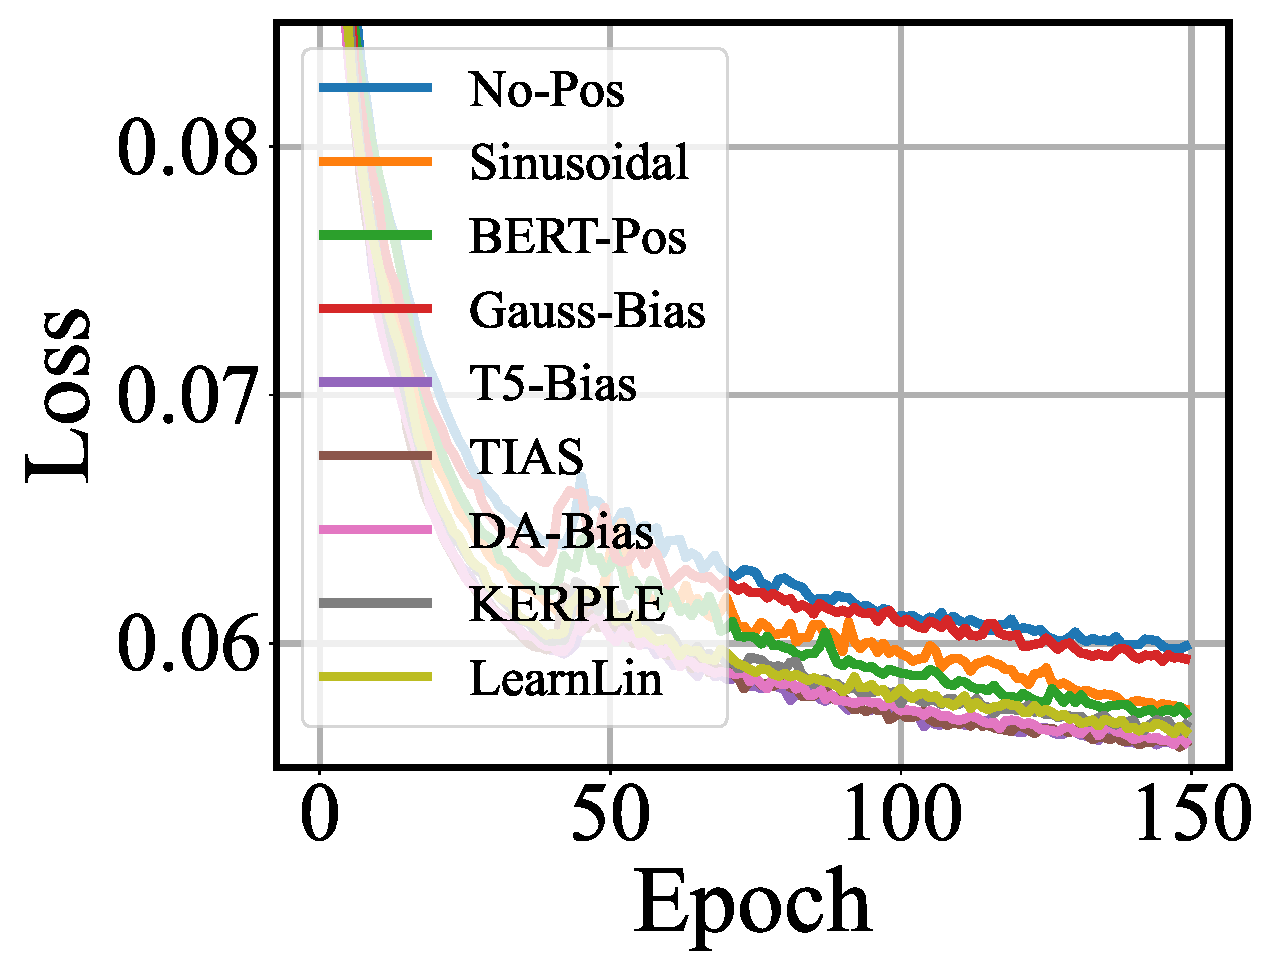
\includegraphics[width=\columnwidth]{./loss_curves/Fig7a.pdf}}
\caption{}
\end{subfigure}\hfill
\begin{subfigure}[t]{0.5\columnwidth}
\centerline{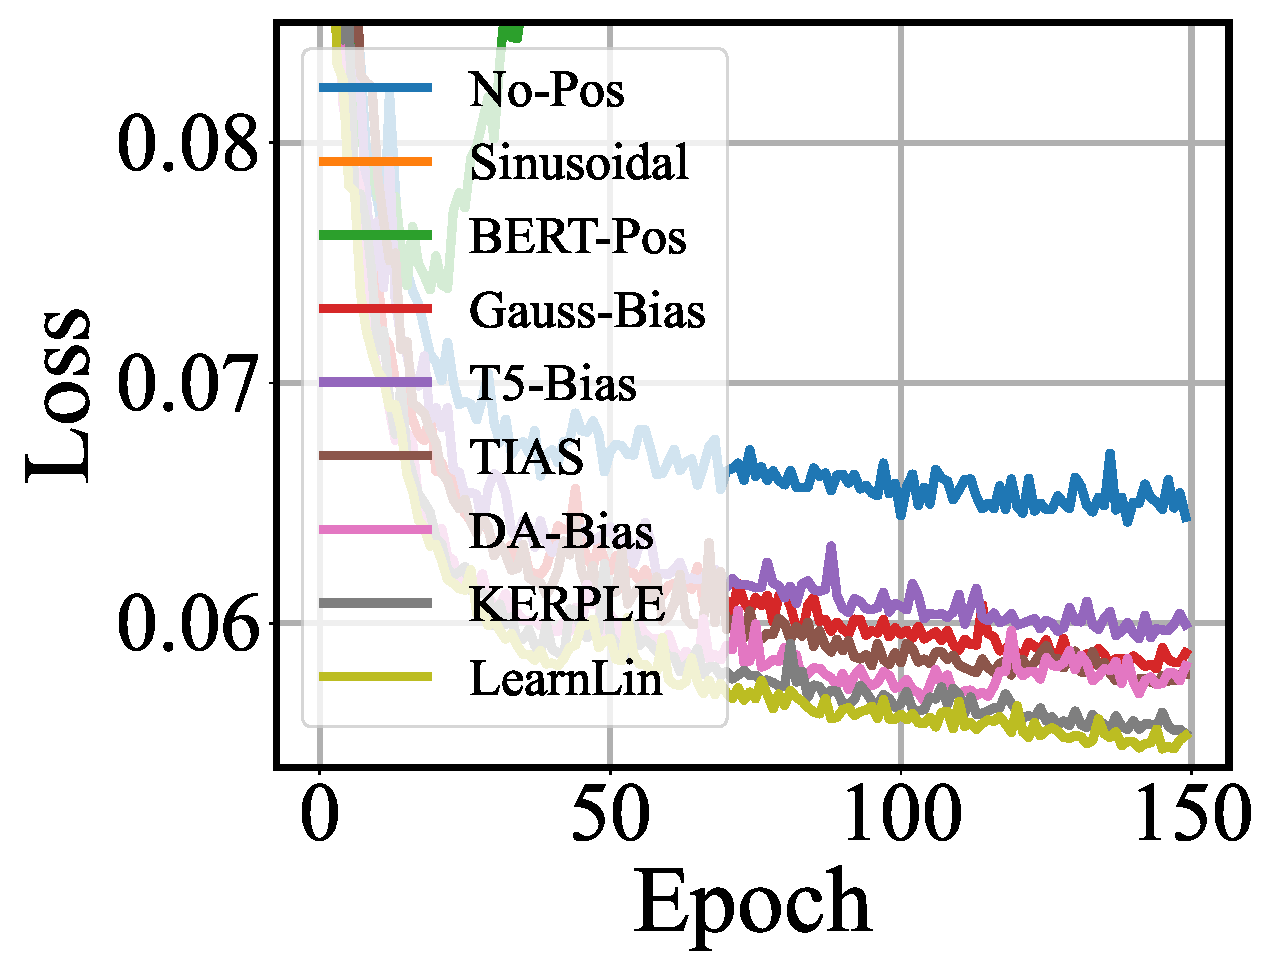
\includegraphics[width=\columnwidth]{./loss_curves/Fig7b.pdf}}
\caption{}
\end{subfigure}
\caption{The (a) training loss and (b) validation loss of the models trained using 2s utterances, on PSM training objective. }
\vskip -1.1em
\label{train2s_MagPSM}
\end{figure}

\subsection{Training and Validation Loss}\label{sec:5.1}
In this section, we first observe the training and validation loss values across the models. The loss curves of different models trained with 1s and 2s speech utterances are given in \textcolor{blue}{Fig.~\ref{train1s_MagMag} (MS)} and Fig.~\ref{train2s_MagIRM}-\ref{train2s_MagPSM} (IRM and PSM), respectively, where 150 epochs are used for training models. Similar trends of loss curves are observed on different training objectives for the same training length. 

% \begin{table}[!ht]
%     \centering
%     \scriptsize
%     \def\arraystretch{0.99}
%     \setlength{\tabcolsep}{5.5pt}
%     % \footnotesize	
%     \caption{Average CBAK scores for each SNR condition and the highest CBAK scores are highlighted in boldface.}
%     \label{tab:cbak}
%     % \vspace*{0.1in}
%     \begin{tabular}{@{}cl||ccccc@{}}
%         \hline
%         &  & \multicolumn{5}{c}{\textbf{Input SNR (dB)}}\\  
%         \cline{3-7}
%         Objective & Network & -5 & 0 & 5 & 10 & 15 \\
%         \hline
%         - & Noisy & 1.15 & 1.40 & 1.58 & 2.13 & 2.61 \\
%         \hline
%         \hline
%         \multirow{8}{*}{IRM}
%         & ResTCN & 1.69 & 2.03 & 2.41 & 2.85 & 3.30 \\
%         & +FA    & 1.75 & 2.10 & 2.50 & 2.94 & 3.39 \\
%         & +TA    & 1.74 & 2.09 & 2.51 & 2.95 & 3.38 \\
%         & +TFA   & \textbf{1.79} & \textbf{2.15} & \textbf{2.56} & \textbf{2.99} & \textbf{3.42} \\
%         \cline{2-7}
%         & MHANet & 1.69 & 2.03 & 2.43 & 2.86 & 3.31 \\
%         & +FA    & 1.75 & 2.10 & 2.50 & 2.93 & 3.36 \\
%         & +TA    & 1.73 & 2.10 & 2.50 & 2.94 & 3.37 \\
%         & +TFA   & \textbf{1.79} & \textbf{2.14} & \textbf{2.55} & \textbf{2.98} & \textbf{3.42} \\
%         \hline
%         \hline
        
%         \multirow{8}{*}{SMM}
%         & ResTCN & 1.71 & 2.04 & 2.41 & 2.81 & 3.23\\
%         & +FA    & 1.78 & 2.14 & 2.53 & 2.96 & 3.39\\
%         & +TA    & 1.77 & 2.13 & 2.53 & 2.96 & 3.39\\
%         & +TFA   & \textbf{1.85} & \textbf{2.21} & \textbf{2.60} & \textbf{3.04} & \textbf{3.46} \\
%         \cline{2-7}
%         & MHANet & 1.72 & 2.07 & 2.46 & 2.89 & 3.34 \\
%         & +FA    & 1.77 & 2.14 & 2.54 & 2.97 & 3.39 \\
%         & +TA    & 1.80 & 2.16 & 2.56 & 2.94 & 3.41\\
%         & +TFA   & \textbf{1.83} & \textbf{2.20} & \textbf{2.60} & \textbf{3.03} & \textbf{3.45} \\
%         \hline
%         \hline
        
%         \multirow{8}{*}{PSM}
%         & ResTCN & 1.70 & 2.07 & 2.49 & 2.94 & 3.41 \\
%         & +FA    & 1.78 & 2.15 & 2.58 & 3.03 & 3.49 \\
%         & +TA    & 1.73 & 2.12 & 2.55 & 3.01 & 3.46 \\
%         & +TFA   & \textbf{1.80} & \textbf{2.19} & \textbf{2.62} & \textbf{3.08} & \textbf{3.53} \\
%         \cline{2-7}
%         & MHANet & 1.60 & 2.08 & 2.51 & 2.98 & 3.44 \\
%         & +FA    & 1.78 & 2.15 & 2.57 & 3.02 & 3.48 \\
%         & +TA    & 1.75 & 2.13 & 2.56 & 3.02 & 3.48 \\
%         & +TFA   & \textbf{1.80} & \textbf{2.19} & \textbf{2.61} & \textbf{3.06} & \textbf{3.49} \\
%         \hline
%         \hline
        
%         \multirow{8}{*}{Xi}
%         & ResTCN & 1.75 & 2.11 & 2.50 & 2.95 & 3.39 \\
%         & +FA    & 1.85 & 2.21 & 2.61 & 3.06 & 3.50 \\
%         & +TA    & 1.85 & 2.21 & 2.61 & 3.05 & 3.49 \\
%         & +TFA   & \textbf{1.90} & \textbf{2.26} & \textbf{2.67} & \textbf{3.11} & \textbf{3.53} \\
%         \cline{2-7}
%         & MHANet & 1.78 & 2.15 & 2.50 & 3.01 & 3.46 \\
%         & +FA    & 1.85 & 2.21 & 2.52 & 3.06 & 3.50 \\
%         & +TA    & 1.82 & 2.19 & 2.54 & 3.04 & 3.47 \\
%         & +TFA   & \textbf{1.88} & \textbf{2.24} & \textbf{2.59} & \textbf{3.09} & \textbf{3.51}\\
%         \hline
%     \end{tabular}
%     % \vspace{-2.0em}
% \end{table}

% \begin{table}[!b]
%     \centering
%     \scriptsize
%     \small
%     % \def\arraystretch{1.05}
%     \def\arraystretch{0.83}
%     \setlength{\tabcolsep}{3.3pt}
%     % \footnotesize	
%     % \caption{Average CSIG scores for each SNR level and the highest CSIG scores are highlighted in boldface.}
%     \caption{Performance evaluation results in terms of PESQ, ESTOI (in \%), CSIG, CBAK, and COVL. All the models are trained (MS as the training objective) with 1s noisy-clean speech pairs and tested on noisy speech utterances of 1s, 5s, 10s, 15s, and 20s in length.}
%     \label{tab:magmag1s}
%     % \vspace*{0.1in}
%     \begin{tabular}{@{}cl||ccccc@{}}
%         \hline
%          % &  & \multicolumn{5}{c}{\textbf{Input SNR (dB)}}\\  
%          &  & \multicolumn{5}{c}{\textbf{Metrics}}\\  
%         \cline{3-7}
%         Test Len. & Model & PESQ & ESTOI & CSIG & CBAK & COVL \\  
%         % \hline
%         % Objective & Network & -5 & 0 & 5 & 10 & 15 \\
%         % \hline
%         \hline
%         \hline
%         \multirow{10}{*}{1s}
%         & Noisy    & 1.98 & 54.81 & 2.39 & 1.88 & 1.76 \\
%         % \cline{2-7}
%         \cdashline{2-7}
%         & No-Pos       & 2.56 & 66.58 & 3.15 & 2.45 & 2.47  \\
%         & Sinusoidal   & 2.68 & 70.19 & 3.27 & 2.53 & 2.58  \\
%         & BERT-Pos     & 2.69 & 70.15 & 3.26 & 2.53 & 2.58  \\
%         & Gauss-Bias   & 2.60 & 67.59 & 3.18 & 2.47 & 2.49  \\
%         & T5-Bias      & 2.70 & 70.27 & 2.29 & \textbf{2.55} & \textbf{2.61}  \\
%         & TISA         & \textbf{2.71} & \textbf{70.72} & \textbf{3.30} & 2.54 & \textbf{2.61}  \\
%         & \textcolor{black}{DA-Bias}           & 2.70 & 70.09 & 3.27 & 2.53 & 2.59  \\
%         & \textcolor{black}{KERPLE}       & 2.69 & 69.85 & 3.28 & 2.51 & 2.58  \\
%         & LearnLin     & \textbf{2.71} & 70.24 & 3.28 & 2.54 & 2.60 \\
%         \hline
%         \hline
%         \multirow{10}{*}{5s}
%         & Noisy    & 1.88 & 54.26 & 2.33 & 1.86 & 1.71 \\
%         % \cline{2-7}
%         \cdashline{2-7}
%         & No-Pos       & 2.42 & 64.24 & 3.05 & 2.34 & 2.34  \\
%         & Sinusoidal   & 2.17 & 56.64 & 2.75 & 2.17 & 2.08  \\
%         % & BERT-Pos     & 2.29 & 59.96 & 2.91 & 2.24 & 2.19  \\
%         & BERT-Pos     & 1.96 & 51.86 & 2.60 & 2.02 & 1.92  \\
%         & Gauss-Bias   & 2.50 & 65.66 & 3.14 & 2.41 & 2.42  \\
%         & T5-Bias      & 2.36 & 62.27 & 2.94 & 2.27 & 2.23  \\
%         & TISA         & 2.65 & 68.60 & 3.27 & 2.49 & 2.55  \\
%         & \textcolor{black}{DA-Bias}           & 2.67 & 69.92 & 3.28 & 2.53 & 2.58  \\
%         & \textcolor{black}{KERPLE}       & 2.67 & 70.40 & 3.29 & 2.50 & 2.57  \\
%         & LearnLin     & \textbf{2.70} & \textbf{70.91} & \textbf{3.31} & \textbf{2.53} & \textbf{2.59} \\
%         \hline
%         \hline
        
%         \multirow{10}{*}{10s}
%         & Noisy    & 1.92 & 53.19 & 2.40 & 1.87 & 1.75 \\
%         % \cline{2-7}
%         \cdashline{2-7}
%         & No-Pos       & 2.38 & 61.48 & 2.99 & 2.29 & 2.28  \\
%         & Sinusoidal   & 2.11 & 52.17 & 2.66 & 2.08 & 2.01  \\
%         % & BERT-Pos     & 2.18 & 54.26 & 2.76 & 2.14 & 2.08  \\
%         & BERT-Pos     & 1.92 & 47.91 & 2.55 & 1.96 & 1.89  \\
%         & Gauss-Bias   & 2.51 & 63.68 & 3.12 & 2.39 & 2.41  \\
%         & T5-Bias      & 2.27 & 57.54 & 2.81 & 2.16 & 2.09  \\
%         & TISA         & 2.56 & 63.18 & 3.08 & 2.38 & 2.39  \\
%         & \textcolor{black}{DA-Bias}           & 2.64 & 66.69 & 3.25 & 2.49 & 2.55  \\
%         & \textcolor{black}{KERPLE}       & 2.68 & 68.31 & 3.29 & 2.51 & 2.59  \\
%         & LearnLin     & \textbf{2.71} & \textbf{69.11} & \textbf{3.32} & \textbf{2.55} & \textbf{2.62}  \\
%         \hline
%         \hline
        
%         \multirow{10}{*}{15s}
%         & Noisy        & 1.90 & 52.68 & 2.32 & 1.83 & 1.71 \\
%         \cdashline{2-7}
%         & No-Pos       & 2.32 & 60.19 & 2.93 & 2.26 & 2.23  \\
%         & Sinusoidal   & 2.05 & 50.80 & 2.57 & 2.02 & 1.93  \\
%         % & BERT-Pos     & 2.14 & 52.44 & 2.69 & 2.07 & 2.02  \\
%         & BERT-Pos   & 1.97 & 47.03 & 2.47 & 1.93 & 1.85  \\
%         & Gauss-Bias   & 2.48 & 63.54 & 3.06 & 2.36 & 2.37  \\
%         & T5-Bias      & 2.22 & 55.74 & 2.74 & 2.11 & 2.05  \\
%         & TISA         & 2.47 & 60.33 & 2.93 & 2.30 & 2.26  \\
%         & \textcolor{black}{DA-Bias}           & 2.58 & 65.65 & 3.18 & 2.45 & 2.49  \\
%         & \textcolor{black}{KERPLE}       & 2.64 & 68.39 & 3.23 & 2.47 & 2.53  \\
%         & LearnLin     & \textbf{2.68} & \textbf{68.93} & \textbf{3.28} & \textbf{2.49} & \textbf{2.57}  \\
%         \hline
%         \hline
        
%         \multirow{10}{*}{20s}
%         & Noisy        & 1.91 & 51.42 & 2.36 & 1.82 & 1.72    \\
%         % \cline{2-7}
%         \cdashline{2-7}
%         & No-Pos       & 2.34 & 59.07 & 2.98 & 2.28 & 2.26  \\
%         & Sinusoidal   & 2.03 & 49.02 & 2.62 & 2.02 & 1.94  \\
%         % & BERT-Pos     & 2.13 & 50.18 & 2.71 & 2.09 & 2.03  \\
%         & BERT-Pos   & 1.91 & 45.23 & 2.50 & 1.91 & 1.84 \\
%         & Gauss-Bias   & 2.53 & 62.39 & 3.15 & 2.41 & 2.42  \\
%         & T5-Bias      & 2.24 & 54.12 & 2.74 & 2.12 & 2.05  \\
%         & TISA         & 2.44 & 57.41 & 2.92 & 2.28 & 2.22  \\
%         & \textcolor{black}{DA-Bias}      & 2.58 & 63.50 & 3.21 & 2.47 & 2.50  \\
%         & \textcolor{black}{KERPLE}       & 2.69 & 67.25 & 3.32 & 2.53 & 2.60  \\
%         & LearnLin     & \textbf{2.72} & \textbf{67.92} & \textbf{3.34} & \textbf{2.56} & \textbf{2.62}  \\
%         \hline
%     \end{tabular}
%     \vspace{-1.5em}
% \end{table}


\begin{table}[!t]
    \centering
    \scriptsize
    \small
    % \def\arraystretch{1.05}
    % \def\arraystretch{0.60}
    % \setlength{\tabcolsep}{3.3pt}
    \def\arraystretch{0.91}
    \setlength{\tabcolsep}{3.3pt}
    \setlength{\abovetopsep}{0pt}
    \setlength\belowbottomsep{0pt} 
    \setlength\aboverulesep{0pt} 
    \setlength\belowrulesep{0pt}
    % \footnotesize	
    % \caption{Average CSIG scores for each SNR level and the highest CSIG scores are highlighted in boldface.}
    \caption{Performance evaluation results in terms of PESQ, ESTOI (in \%), CSIG, CBAK, and COVL. All the models are trained (MS as the training objective) with 1s noisy-clean speech pairs and tested on noisy speech utterances of 1s, 5s, 10s, 15s, and 20s in length.}
    \label{tab:magmag1s}
    % \vspace*{0.1in}
    \begin{tabular}{@{}cl||ccccc@{}}
        % \hline
        \toprule[1.25pt]
         % &  & \multicolumn{5}{c}{\textbf{Input SNR (dB)}}\\  
         &  & \multicolumn{5}{c}{\textbf{Metrics}}\\  
        % \cline{3-7}
        Test Len. & Model & PESQ & ESTOI & CSIG & CBAK & COVL \\  
        % \hline
        % Objective & Network & -5 & 0 & 5 & 10 & 15 \\
        % \hline
        \hline
        \hline
        \multirow{10}{*}{1s}
        & Noisy    & 1.98 & 54.81 & 2.39 & 1.88 & 1.76 \\
        % \cline{2-7}
        \cdashline{2-7}
        & No-Pos       & 2.56 & 66.58 & 3.15 & 2.45 & 2.47  \\
        & Sinusoidal   & 2.68 & 70.19 & 3.27 & 2.53 & 2.58  \\
        & BERT-Pos     & 2.69 & 70.15 & 3.26 & 2.53 & 2.58  \\
        & Gauss-Bias   & 2.60 & 67.59 & 3.18 & 2.47 & 2.49  \\
        & T5-Bias      & 2.70 & 70.27 & 3.29 & \textbf{2.55} & \textbf{2.61}  \\
        & TISA         & \textbf{2.71} & \textbf{70.72} & \textbf{3.30} & 2.54 & \textbf{2.61}  \\
        & \textcolor{black}{DA-Bias}           & 2.70 & 70.09 & 3.27 & 2.53 & 2.59  \\
        & \textcolor{black}{KERPLE}       & 2.69 & 69.85 & 3.28 & 2.51 & 2.58  \\
        & LearnLin     & \textbf{2.71} & 70.24 & 3.28 & 2.54 & 2.60 \\
        \hline
        \hline
        \multirow{10}{*}{5s}
        & Noisy    & 1.88 & 54.26 & 2.33 & 1.86 & 1.71 \\
        % \cline{2-7}
        \cdashline{2-7}
        & No-Pos       & 2.42 & 64.24 & 3.05 & 2.34 & 2.34  \\
        & Sinusoidal   & 2.19 & 57.17 & 2.77 & 2.17 & 2.09  \\
        % & BERT-Pos     & 2.29 & 59.40 & 2.89 & 2.23 & 2.18  \\
        & BERT-Pos     & 1.96 & 51.86 & 2.60 & 2.02 & 1.92  \\
        & Gauss-Bias   & 2.50 & 65.66 & 3.14 & 2.41 & 2.42  \\
        & T5-Bias      & 2.36 & 62.27 & 2.95 & 2.27 & 2.24  \\
        & TISA         & 2.65 & 68.60 & 3.27 & 2.49 & 2.55  \\
        & \textcolor{black}{DA-Bias}           & 2.67 & 69.92 & 3.28 & 2.53 & 2.58  \\
        & \textcolor{black}{KERPLE}       & 2.67 & 70.40 & 3.29 & 2.50 & 2.57  \\
        & LearnLin     & \textbf{2.70} & \textbf{70.91} & \textbf{3.31} & \textbf{2.53} & \textbf{2.59} \\
        \hline
        \hline
        
        \multirow{10}{*}{10s}
        & Noisy    & 1.92 & 53.19 & 2.40 & 1.87 & 1.75 \\
        % \cline{2-7}
        \cdashline{2-7}
        & No-Pos       & 2.38 & 61.48 & 2.99 & 2.29 & 2.28  \\
        & Sinusoidal   & 2.11 & 52.17 & 2.67 & 2.09 & 2.01  \\
        % & BERT-Pos     & 2.17 & 53.56 & 2.72 & 2.14 & 2.05  \\
        & BERT-Pos     & 1.92 & 47.91 & 2.55 & 1.96 & 1.89  \\
        & Gauss-Bias   & 2.51 & 63.68 & 3.12 & 2.39 & 2.41  \\
        & T5-Bias      & 2.27 & 57.54 & 2.82 & 2.17 & 2.12  \\
        & TISA         & 2.56 & 63.18 & 3.08 & 2.38 & 2.39  \\
        & \textcolor{black}{DA-Bias}           & 2.64 & 66.69 & 3.25 & 2.49 & 2.55  \\
        & \textcolor{black}{KERPLE}       & 2.68 & 68.31 & 3.29 & 2.51 & 2.59  \\
        & LearnLin     & \textbf{2.71} & \textbf{69.11} & \textbf{3.32} & \textbf{2.55} & \textbf{2.62}  \\
        \hline
        \hline
        
        \multirow{10}{*}{15s}
        & Noisy        & 1.90 & 52.68 & 2.32 & 1.83 & 1.71 \\
        \cdashline{2-7}
        & No-Pos       & 2.32 & 60.19 & 2.93 & 2.26 & 2.23  \\
        & Sinusoidal    & 2.05 & 50.80 & 2.57 & 2.03 & 1.94  \\
        % & BERT-Pos     & 2.13 & 51.72 & 2.65 & 2.07 & 1.99  \\
        & BERT-Pos   & 1.97 & 47.03 & 2.47 & 1.93 & 1.85  \\
        & Gauss-Bias   & 2.48 & 63.54 & 3.06 & 2.36 & 2.37  \\
        & T5-Bias      & 2.23 & 58.30 & 2.82 & 2.23 & 2.11  \\
        & TISA         & 2.47 & 60.33 & 2.93 & 2.30 & 2.26  \\
        & \textcolor{black}{DA-Bias}           & 2.58 & 65.65 & 3.18 & 2.45 & 2.49  \\
        & \textcolor{black}{KERPLE}       & 2.64 & 68.39 & 3.23 & 2.47 & 2.53  \\
        & LearnLin     & \textbf{2.68} & \textbf{68.93} & \textbf{3.28} & \textbf{2.49} & \textbf{2.57}  \\
        \hline
        \hline
        
        \multirow{10}{*}{20s}
        & Noisy        & 1.91 & 51.42 & 2.36 & 1.82 & 1.72    \\
        % \cline{2-7}
        \cdashline{2-7}
        & No-Pos       & 2.34 & 59.07 & 2.98 & 2.28 & 2.26  \\
        & Sinusoidal   & 2.03 & 49.02 & 2.62 & 2.02 & 1.94  \\
        % & BERT-Pos     & 2.131.99 & 497.5137 & 2.662 & 2.082 & 1.994  \\
        & BERT-Pos     & 1.91 & 45.23 & 2.50 & 1.91 & 1.84 \\
        & Gauss-Bias   & 2.53 & 62.39 & 3.15 & 2.41 & 2.42  \\
        & T5-Bias      & 2.25 & 54.56 & 2.80 & 2.14 & 2.09  \\
        & TISA         & 2.44 & 57.41 & 2.92 & 2.28 & 2.22  \\
        & \textcolor{black}{DA-Bias}      & 2.58 & 63.50 & 3.21 & 2.47 & 2.50  \\
        & \textcolor{black}{KERPLE}       & 2.69 & 67.25 & 3.32 & 2.53 & 2.60  \\
        & LearnLin     & \textbf{2.72} & \textbf{67.92} & \textbf{3.34} & \textbf{2.56} & \textbf{2.62}  \\
        % \hline
        \toprule[1.25pt]
    \end{tabular}
    \vspace{-2.0em}
\end{table}

% \begin{table}[!b]
%     \centering
%     \scriptsize
%     \small
%     % \def\arraystretch{1.05}
%     \def\arraystretch{0.83}
%     \setlength{\tabcolsep}{3.3pt}
%     % \footnotesize	
%     % \caption{Average CSIG scores for each SNR level and the highest CSIG scores are highlighted in boldface.}
%     \caption{Performance evaluation results in terms of PESQ, ESTOI (in \%), CSIG, CBAK, and COVL. All the models are trained (IRM as the training objective) with 1s noisy-clean speech pairs and tested on noisy speech utterances with lengths of 1s, 5s, 10s, 15s, and 20s.}
%     \label{tab:magirm1s}
%     % \vspace*{0.1in}
%     \begin{tabular}{@{}cl||ccccc@{}}
%         \hline
%          % &  & \multicolumn{5}{c}{\textbf{Input SNR (dB)}}\\  
%          &  & \multicolumn{5}{c}{\textbf{Metrics}}\\  
%         \cline{3-7}
%         Test Len. & Model & PESQ & ESTOI & CSIG & CBAK & COVL\\  
%         % \hline
%         % Objective & Network & -5 & 0 & 5 & 10 & 15 \\
%         % \hline
%         \hline
%         \hline
%         \multirow{10}{*}{1s}
%         & Noisy    & 1.98 & 54.81 & 2.39 & 1.88 & 1.76 \\
%         % \cline{2-7}
%         \cdashline{2-7}
%         & No-Pos      & 2.48 & 67.23 & 3.12 & 2.51 & 2.39  \\
%         & Sinusoidal   & 2.57 & 70.21 & 3.23 & 2.56 & 2.48  \\
%         & BERT-Pos     & 2.58 & 70.61 & 3.22 & 2.58 & 2.49  \\
%         & Gauss-Bias   & 2.50 & 67.61 & 3.15 & 2.54 & 2.41  \\
%         & T5-Bias      & \textbf{2.60} & \textbf{71.04} & \textbf{3.26} & \textbf{2.59} & \textbf{2.51}  \\
%         & TISA         & \textbf{2.60} & 70.86 & \textbf{3.26} & \textbf{2.59} & 2.50  \\
%         & \textcolor{black}{DA-Bias}   & 2.58 & 70.65 & 3.25 & 2.57 & 2.50  \\
%         & \textcolor{black}{KERPLE}       & 2.57 & 70.13 & 3.24 & 2.57 & 2.49  \\
%         & LearnLin     & 2.59 & 71.01 & 3.25 & \textbf{2.59} & 2.50  \\
%         % & +TA & 2.33 & 2.83 & 3.28 & 3.72 & 4.12 \\
%         % & +TFA & \textbf{2.37} & \textbf{2.85} & \textbf{3.32} & \textbf{3.77} & \textbf{4.18}\\
%         \hline
%         \hline
%         \multirow{10}{*}{5s}
%         & Noisy    & 1.88 & 54.26 & 2.33 & 1.86 & 1.71 \\
%         % \cline{2-7}
%         \cdashline{2-7}
%         & No-Pos       & 2.33 & 64.56 & 2.98 & 2.39 & 2.25  \\
%         & Sinusoidal   & 2.17 & 56.22 & 2.73 & 2.24 & 2.03  \\
%         % & BERT-Pos     & 2.26 & 61.48 & 2.92 & 2.34 & 2.19  \\
%         & BERT-Pos     & 1.99 & 52.96 & 2.53 & 2.12 & 1.89  \\
%         & Gauss-Bias   & 2.42 & 66.43 & 3.09 & 2.48 & 2.34  \\
%         & T5-Bias      & 2.31 & 64.06 & 2.97 & 2.37 & 2.23  \\
%         & TISA         & 2.53 & 69.87 & 3.22 & 2.54 & 2.46  \\
%         & \textcolor{black}{DA-Bias}   & 2.53 & 69.19 & 3.23 & 2.55 & 2.48  \\
%         & \textcolor{black}{KERPLE}       & 2.54 & 70.29 & 3.23 & 2.55 & 2.47  \\
%         & LearnLin     & \textbf{2.57} & \textbf{70.48} & \textbf{3.25} & \textbf{2.57} & \textbf{2.50} \\
%         % & +TA & 2.33 & 2.83 & 3.28 & 3.72 & 4.12 \\
%         % & +TFA & \textbf{2.37} & \textbf{2.85} & \textbf{3.32} & \textbf{3.77} & \textbf{4.18}\\
%         \hline
%         \hline
        
%         \multirow{10}{*}{10s}
%         & Noisy    & 1.92 & 53.19 & 2.40 & 1.87 & 1.75 \\
%         % \cline{2-7}
%         \cdashline{2-7}
%         & No-Pos       & 2.32 & 62.48 & 2.99 & 2.35 & 2.24  \\
%         & Sinusoidal   & 2.11 & 50.74 & 2.62 & 2.14 & 1.97  \\
%         % & BERT-Pos     & 2.16 & 56.97 & 2.83 & 2.25 & 2.10  \\
%         & BERT-Pos     & 1.97 & 50.64 & 2.44 & 2.05 & 1.83  \\
%         & Gauss-Bias   & 2.44 & 64.62 & 3.14 & 2.46 & 2.37  \\
%         & T5-Bias      & 2.27 & 59.46 & 2.91 & 2.28 & 2.17  \\
%         & TISA         & 2.51 & 66.98 & 3.19 & 2.49 & 2.43  \\
%         & \textcolor{black}{DA-Bias}   & 2.50 & 66.32 & 3.22 & 2.50 & 2.46  \\
%         & \textcolor{black}{KERPLE}       & 2.56 & 68.62 & 3.27 & 2.54 & 2.50  \\
%         & LearnLin     & \textbf{2.59} & \textbf{68.89} & \textbf{3.29} & \textbf{2.56} & \textbf{2.53}  \\
        
%         % & ResTCN & 2.10 & 2.59 & 3.06 & 3.51 & 3.94\\
%         % & +FA    & 2.30 & 2.80 & 3.27 & 3.73 & 4.14\\
%         % & +TA    & 2.29 & 2.80 & 3.28 & 3.74 & 4.14\\
%         % & +TFA   & \textbf{2.37} & \textbf{2.90} & \textbf{3.37} & \textbf{3.81} & \textbf{4.20}\\
%         % \cline{2-7}
%         % & MHANet & 2.21 & 2.70 & 3.17 & 3.63 & 4.06 \\
%         % & +FA    & 2.27 & 2.76 & 3.24 & 3.69 & 4.10 \\
%         % & +TA    & 2.30 & 2.81 & 3.29 & 3.74 & 4.15 \\
%         % & +TFA   & \textbf{2.36} & \textbf{2.86} & \textbf{3.34} & \textbf{3.78} & \textbf{4.18}\\
%         \hline
%         \hline
        
%         \multirow{10}{*}{15s}
%         & Noisy        & 1.90 & 52.68 & 2.32 & 1.83 & 1.71 \\
%         \cdashline{2-7}
%         & No-Pos       & 2.27 & 61.63 & 2.89 & 2.30 & 2.17  \\
%         & Sinusoidal   & 2.11 & 49.39 & 2.54 & 2.10 & 1.93  \\
%         % & BERT-Pos     & 2.12 & 55.02 & 2.73 & 2.18 & 2.03  \\
%         & BERT-Pos   & 1.92 & 49.68 & 2.39 & 2.01 & 1.79  \\
%         & Gauss-Bias   & 2.40 & 64.21 & 3.06 & 2.42 & 2.32  \\
%         & T5-Bias      & 2.21 & 58.30 & 2.81 & 2.22 & 2.09  \\
%         & TISA         & 2.43 & 65.59 & 3.08 & 2.42 & 2.34  \\
%         & \textcolor{black}{DA-Bias}   & 2.44 & 65.05 & 3.12 & 2.44 & 2.37  \\
%         & \textcolor{black}{KERPLE}       & 2.52 & 68.31 & 3.20 & 2.49 & 2.45  \\
%         & LearnLin     & \textbf{2.55} & \textbf{68.61} & \textbf{3.23} & \textbf{2.53} & \textbf{2.48}  \\
%         % & ResTCN & 2.15 & 2.65 & 3.13 & 3.61 & 4.06 \\
%         % & +FA    & 2.30 & 2.78 & 3.26 & 3.74 & 4.18 \\
%         % & +TA    & 2.29 & 2.81 & 3.30 & 3.77 & 4.20 \\
%         % & +TFA   & \textbf{2.38} & \textbf{2.88} & \textbf{3.36} & \textbf{3.80} & \textbf{4.21} \\
%         % \cline{2-7}
%         % & MHANet & 2.22 & 2.73 & 3.23 & 3.73 & 4.16 \\
%         % & +FA    & 2.29 & 2.78 & 3.28 & 3.76 & 4.19 \\
%         % & +TA    & 2.30 & 2.80 & 3.30 & 3.78 & 4.22 \\
%         % & +TFA   & \textbf{2.36} & \textbf{2.86} & \textbf{3.35} & \textbf{3.82} & \textbf{4.23} \\
%         \hline
%         \hline
        
%         \multirow{10}{*}{20s}
%         & Noisy        & 1.91 & 51.42 & 2.36 & 1.82 & 1.72    \\
%         % \cline{2-7}
%         \cdashline{2-7}
%         & No-Pos       & 2.29 & 60.33 & 2.95 & 2.32 & 2.21  \\
%         & Sinusoidal   & 2.14 & 47.65 & 2.53 & 2.09 & 1.92  \\
%         % & BERT-Pos     & 2.11 & 53.15 & 2.75 & 2.16 & 2.03  \\
%         & BERT-Pos     & 1.92 & 48.53 & 2.42 & 1.99 & 1.79  \\
%         & Gauss-Bias   & 2.44 & 63.43 & 3.13 & 2.45 & 2.37  \\
%         & T5-Bias      & 2.21 & 56.31 & 2.83 & 2.21 & 2.10  \\
%         & TISA         & 2.45 & 63.53 & 3.11 & 2.42 & 2.36  \\
%         & \textcolor{black}{DA-Bias}   & 2.44 & 63.05 & 3.15 & 2.44 & 2.39  \\
%         & \textcolor{black}{KERPLE}       & 2.55 & 67.28 & 3.27 & 2.53 & 2.49  \\
%         & LearnLin     & \textbf{2.58} & \textbf{67.51} & \textbf{3.29} & \textbf{2.55} & \textbf{2.52}  \\
%         % & ResTCN & 2.19 & 2.70 & 3.16 & 3.63 & 4.05 \\
%         % & +FA    & 2.32 & 2.79 & 3.27 & 3.76 & 4.19 \\
%         % & +TA    & 2.29 & 2.80 & 3.28 & 3.75 & 4.18 \\
%         % & +TFA   & \textbf{2.41} & \textbf{2.91} & \textbf{3.37} & \textbf{3.84} & \textbf{4.23} \\
%         % \cline{2-7}
%         % & MHANet & 2.26 & 2.77 & 3.25 & 3.72 & 4.16\\
%         % & +FA    & 2.33 & 2.82 & 3.27 & 3.75 & \textbf{4.18} \\
%         % & +TA    & 2.31 & 2.83 & 3.30 & 3.76 & 4.17\\
%         % & +TFA   & \textbf{2.37} & \textbf{2.86} & \textbf{3.34} & \textbf{3.79} & \textbf{4.18} \\
%         \hline
%     \end{tabular}
%     \vspace{-1.5em}
% \end{table}


\begin{table}[!h]
    \centering
    \scriptsize
    \small
    % \def\arraystretch{1.05}
    % \def\arraystretch{0.57}
    % \setlength{\tabcolsep}{3.3pt}
    \def\arraystretch{0.91}
    \setlength{\tabcolsep}{3.3pt}
    \setlength{\abovetopsep}{0pt}
    \setlength\belowbottomsep{0pt} 
    \setlength\aboverulesep{0pt} 
    \setlength\belowrulesep{0pt}
    % \footnotesize	
    % \caption{Average CSIG scores for each SNR level and the highest CSIG scores are highlighted in boldface.}
    \caption{Performance evaluation results in terms of PESQ, ESTOI (in \%), CSIG, CBAK, and COVL. All the models are trained (IRM as the training objective) with 1s noisy-clean speech pairs and tested on noisy speech utterances with lengths of 1s, 5s, 10s, 15s, and 20s.}
    \label{tab:magirm1s}
    % \vspace*{0.1in}
    \begin{tabular}{@{}cl||ccccc@{}}
        \toprule[1.25pt]
         % \hline
         % &  & \multicolumn{5}{c}{\textbf{Input SNR (dB)}}\\  
         &  & \multicolumn{5}{c}{\textbf{Metrics}}\\  
        % \cline{3-7}
        Test Len. & Model & PESQ & ESTOI & CSIG & CBAK & COVL\\  
        % \hline
        % Objective & Network & -5 & 0 & 5 & 10 & 15 \\
        % \hline
        \hline
        \hline
        \multirow{10}{*}{1s}
        & Noisy    & 1.98 & 54.81 & 2.39 & 1.88 & 1.76 \\
        % \cline{2-7}
        \cdashline{2-7}
        & No-Pos      & 2.48 & 67.23 & 3.12 & 2.51 & 2.39  \\
        & Sinusoidal   & 2.57 & 70.21 & 3.23 & 2.56 & 2.48  \\
        & BERT-Pos     & 2.58 & 70.61 & 3.22 & 2.58 & 2.49  \\
        & Gauss-Bias   & 2.50 & 67.61 & 3.15 & 2.54 & 2.41  \\
        & T5-Bias      & \textbf{2.60} & \textbf{71.04} & \textbf{3.26} & \textbf{2.59} & \textbf{2.51}  \\
        & TISA         & \textbf{2.60} & 70.86 & \textbf{3.26} & \textbf{2.59} & 2.50  \\
        & \textcolor{black}{DA-Bias}   & 2.58 & 70.65 & 3.25 & 2.57 & 2.50  \\
        & \textcolor{black}{KERPLE}       & 2.57 & 70.13 & 3.24 & 2.57 & 2.49  \\
        & LearnLin     & 2.59 & 71.01 & 3.25 & \textbf{2.59} & 2.50  \\
        % & +TA & 2.33 & 2.83 & 3.28 & 3.72 & 4.12 \\
        % & +TFA & \textbf{2.37} & \textbf{2.85} & \textbf{3.32} & \textbf{3.77} & \textbf{4.18}\\
        \hline
        \hline
        \multirow{10}{*}{5s}
        & Noisy    & 1.88 & 54.26 & 2.33 & 1.86 & 1.71 \\
        % \cline{2-7}
        \cdashline{2-7}
        & No-Pos       & 2.33 & 64.56 & 2.98 & 2.39 & 2.25  \\
        & Sinusoidal   & 2.17 & 56.22 & 2.73 & 2.24 & 2.04  \\
        % & BERT-Pos     & 2.26 & 61.10 & 2.92 & 2.34 & 2.19  \\
        & BERT-Pos     & 1.99 & 52.96 & 2.53 & 2.12 & 1.89  \\
        & Gauss-Bias   & 2.42 & 66.43 & 3.09 & 2.48 & 2.34  \\
        & T5-Bias      & 2.31 & 64.06 & 2.97 & 2.37 & 2.23  \\
        & TISA         & 2.53 & 69.87 & 3.22 & 2.54 & 2.46  \\
        & \textcolor{black}{DA-Bias}   & 2.53 & 69.19 & 3.23 & 2.55 & 2.48  \\
        & \textcolor{black}{KERPLE}       & 2.54 & 70.29 & 3.23 & 2.55 & 2.47  \\
        & LearnLin     & \textbf{2.57} & \textbf{70.48} & \textbf{3.25} & \textbf{2.57} & \textbf{2.50} \\

        \hline
        \hline
        
        \multirow{10}{*}{10s}
        & Noisy    & 1.92 & 53.19 & 2.40 & 1.87 & 1.75 \\
        % \cline{2-7}
        \cdashline{2-7}
        & No-Pos       & 2.32 & 62.48 & 2.99 & 2.35 & 2.24  \\
        & Sinusoidal   & 2.12 & 52.11 & 2.64 & 2.15 & 1.99  \\
        % & BERT-Pos     & 2.15 & 56.08 & 2.81 & 2.24 & 2.09  \\
        & BERT-Pos     & 1.97 & 50.64 & 2.44 & 2.05 & 1.83  \\
        & Gauss-Bias   & 2.44 & 64.62 & 3.14 & 2.46 & 2.37  \\
        & T5-Bias      & 2.28 & 59.92 & 2.92 & 2.29 & 2.17  \\
        & TISA         & 2.51 & 66.98 & 3.19 & 2.49 & 2.43  \\
        & \textcolor{black}{DA-Bias}   & 2.50 & 66.32 & 3.22 & 2.50 & 2.46  \\
        & \textcolor{black}{KERPLE}       & 2.56 & 68.62 & 3.27 & 2.54 & 2.50  \\
        & LearnLin     & \textbf{2.59} & \textbf{68.89} & \textbf{3.29} & \textbf{2.56} & \textbf{2.53}  \\
        
        \hline
        \hline
        
        \multirow{10}{*}{15s}
        & Noisy        & 1.90 & 52.68 & 2.32 & 1.83 & 1.71 \\
        \cdashline{2-7}
        & No-Pos       & 2.27 & 61.63 & 2.89 & 2.30 & 2.17  \\
        & Sinusoidal   & 2.11 & 51.15 & 2.56 & 2.11 & 1.94  \\
        % & BERT-Pos     & 2.10 & 53.93 & 2.71 & 2.17 & 2.01  \\
        & BERT-Pos     & 1.92 & 49.68 & 2.39 & 2.01 & 1.79  \\
        & Gauss-Bias   & 2.40 & 64.21 & 3.06 & 2.42 & 2.32  \\
        & T5-Bias      & 2.23 & 58.30 & 2.82 & 2.23 & 2.11  \\
        & TISA         & 2.43 & 65.59 & 3.08 & 2.42 & 2.34  \\
        & \textcolor{black}{DA-Bias}   & 2.44 & 65.05 & 3.12 & 2.44 & 2.37  \\
        & \textcolor{black}{KERPLE}       & 2.52 & 68.31 & 3.20 & 2.49 & 2.45  \\
        & LearnLin     & \textbf{2.55} & \textbf{68.61} & \textbf{3.23} & \textbf{2.53} & \textbf{2.48}  \\

        \hline
        \hline
        
        \multirow{10}{*}{20s}
        & Noisy        & 1.91 & 51.42 & 2.36 & 1.82 & 1.72    \\
        % \cline{2-7}
        \cdashline{2-7}
        & No-Pos       & 2.29 & 60.33 & 2.95 & 2.32 & 2.21  \\
        & Sinusoidal   & 2.15 & 49.14 & 2.55 & 2.11 & 1.94  \\
        % & BERT-Pos     & 2.08 & 51.998 & 2.72 & 2.15 & 2.01  \\
        & BERT-Pos     & 1.92 & 48.53 & 2.42 & 1.99 & 1.79  \\
        & Gauss-Bias   & 2.44 & 63.43 & 3.13 & 2.45 & 2.37  \\
        & T5-Bias      & 2.24 & 56.94 & 2.85 & 2.23 & 2.12  \\
        & TISA         & 2.45 & 63.53 & 3.11 & 2.42 & 2.36  \\
        & \textcolor{black}{DA-Bias}   & 2.44 & 63.05 & 3.15 & 2.44 & 2.39  \\
        & \textcolor{black}{KERPLE}       & 2.55 & 67.28 & 3.27 & 2.53 & 2.49  \\
        & LearnLin     & \textbf{2.58} & \textbf{67.51} & \textbf{3.29} & \textbf{2.55} & \textbf{2.52}  \\
        % & ResTCN & 2.19 & 2.70 & 3.16 & 3.63 & 4.05 \\
        % & +FA    & 2.32 & 2.79 & 3.27 & 3.76 & 4.19 \\
        % & +TA    & 2.29 & 2.80 & 3.28 & 3.75 & 4.18 \\
        % & +TFA   & \textbf{2.41} & \textbf{2.91} & \textbf{3.37} & \textbf{3.84} & \textbf{4.23} \\
        % \cline{2-7}
        % & MHANet & 2.26 & 2.77 & 3.25 & 3.72 & 4.16\\
        % & +FA    & 2.33 & 2.82 & 3.27 & 3.75 & \textbf{4.18} \\
        % & +TA    & 2.31 & 2.83 & 3.30 & 3.76 & 4.17\\
        % & +TFA   & \textbf{2.37} & \textbf{2.86} & \textbf{3.34} & \textbf{3.79} & \textbf{4.18} \\
        % \hline
        \toprule[1.25pt]
    \end{tabular}
    \vspace{-2.0em}
\end{table}
% % \begin{table}[!b]
%     \centering
%     \scriptsize
%     \small
%     % \def\arraystretch{1.05}
%     \def\arraystretch{0.85}
%     \setlength{\tabcolsep}{3.3pt}
%     % \footnotesize	
%     % \caption{Average CSIG scores for each SNR level and the highest CSIG scores are highlighted in boldface.}
%     \caption{Performance evaluation results in terms of PESQ, ESTOI (in \%), CSIG, CBAK, and COVL. All the models are trained (SMM as the training objective) with 1s noisy-clean speech pairs and tested on noisy speech utterances with lengths of 1s, 5s, 10s, 15s, and 20s.}
%     \label{tab:magsmm1s}
%     % \vspace*{0.1in}
%     \begin{tabular}{@{}cl||ccccc@{}}
%         \hline
%          % &  & \multicolumn{5}{c}{\textbf{Input SNR (dB)}}\\  
%          &  & \multicolumn{5}{c}{\textbf{Metrics}}\\  
%         \cline{3-7}
%         Test Len. & Model & PESQ & ESTOI & CSIG & CBAK & COVL\\  
%         % \hline
%         % Objective & Network & -5 & 0 & 5 & 10 & 15 \\
%         % \hline
%         \hline
%         \hline
%         \multirow{10}{*}{1s}
%         & Noisy    & 1.88 & 54.26 & 2.33 & 1.86 & 1.71 \\
%         % \cline{2-7}
%         \cdashline{2-7}
%         & No-Pos       & 2.48 & 67.30 & 3.14 & 2.54 & 2.41  \\
%         & Sinusoidal   & 2.58 & 70.80 & 3.25 & 2.59 & 2.50  \\
%         & BERT-Pos     & 2.57 & 70.53 & 3.23 & 2.59 & 2.49  \\
%         & Gauss-Bias   & 2.53 & 69.28 & 3.19 & 2.56 & 2.45  \\
%         & T5-Bias      & 2.59 & 71.14 & 3.28 & 2.61 & 2.52  \\
%         & TISA         & \textbf{2.61} & 71.13 & \textbf{3.29} & \textbf{2.62} & \textbf{2.54}  \\
%         & \textcolor{black}{DA-Bias}   & 2.60 & \textbf{71.23} & 3.27 & 2.61 & 2.53  \\
%         & \textcolor{black}{KERPLE}       & 2.58 & 70.60 & 3.25 & 2.60 & 2.51  \\
%         & LearnLin     & 2.59 & 70.82 & 3.27 & 2.61 & 2.53 \\
%         \hline
%         \hline
%         \multirow{10}{*}{5s}
%         & Noisy    & 1.88 & 54.26 & 2.33 & 1.86 & 1.71 \\
%         % \cline{2-7}
%         \cdashline{2-7}
%         & No-Pos       & 2.32 & 64.74 & 2.99 & 2.41 & 2.25  \\
%         & Sinusoidal   & 2.03 & 54.31 & 2.64 & 2.17 & 1.95  \\
%         % & BERT-Pos     & 2.23 & 60.35 & 2.90 & 2.33 & 2.17  \\
%         & BERT-Pos     & 2.02 & 53.19 & 2.64 & 2.14 & 1.94  \\
%         & Gauss-Bias   & 2.38 & 66.33 & 3.06 & 2.47 & 2.32  \\
%         & T5-Bias      & 2.28 & 63.26 & 2.95 & 2.36 & 2.21  \\
%         & TISA         & 2.52 & 70.17 & 3.24 & 2.56 & 2.48  \\
%         & \textcolor{black}{DA-Bias}   & 2.54 & 70.10 & 3.23 & 2.58 & 2.48  \\
%         & \textcolor{black}{KERPLE}       & 2.53 & 70.47 & 3.23 & 2.57 & 2.48  \\
%         & LearnLin     & \textcolor{black}{\textbf{2.57}} & \textcolor{black}{\textbf{71.02}} & \textcolor{black}{\textbf{3.27}} & \textcolor{black}{\textbf{2.60}} & \textcolor{black}{\textbf{2.52}} \\
%         \hline
%         \hline
        
%         \multirow{10}{*}{10s}
%         & Noisy    & 1.92 & 53.19 & 2.40 & 1.87 & 1.75 \\
%         % \cline{2-7}
%         \cdashline{2-7}
%         & No-Pos       & 2.29 & 62.15 & 2.99 & 2.37 & 2.25  \\
%         & Sinusoidal   & 1.93 & 49.85 & 2.53 & 2.06 & 1.87  \\
%         % & BERT-Pos     & 2.11 & 55.51 & 2.79 & 2.22 & 2.07  \\
%         & BERT-Pos     & 1.98 & 50.63 & 2.60 & 2.08 & 1.92  \\
%         & Gauss-Bias   & 2.41 & 64.61 & 3.11 & 2.47 & 2.35  \\
%         & T5-Bias      & 2.22 & 58.75 & 2.89 & 2.26 & 2.14  \\
%         & TISA         & 2.49 & 67.26 & 3.23 & 2.53 & 2.46  \\
%         & \textcolor{black}{DA-Bias}   & 2.51 & 67.39 & 3.23 & 2.55 & 2.47  \\
%         & \textcolor{black}{KERPLE}       & 2.55 & 68.73 & 3.28 & 2.57 & 2.52  \\
%         & LearnLin     & \textbf{2.59} & \textbf{69.34} & \textbf{3.31} & \textbf{2.60} & \textbf{2.56}  \\
%         \hline
%         \hline
        
%         \multirow{10}{*}{15s}
%         & Noisy        & 1.90 & 52.68 & 2.32 & 1.83 & 1.71 \\
%         \cdashline{2-7}
%         & No-Pos       & 2.23 & 61.31 & 2.89 & 2.30 & 2.17  \\
%         & Sinusoidal   & 1.89 & 47.69 & 2.41 & 1.99 & 1.79  \\
%         % & BERT-Pos     & 2.05 & 53.68 & 2.70 & 2.14 & 1.99  \\
%         & BERT-Pos     & 1.97 & 49.21 & 2.56 & 2.04 & 1.89  \\
%         & Gauss-Bias   & 2.37 & 64.34 & 3.03 & 2.43 & 2.30  \\
%         & T5-Bias      & 2.16 & 57.07 & 2.78 & 2.21 & 2.06  \\
%         & TISA         & 2.42 & 65.80 & 3.09 & 2.44 & 2.35  \\
%         & \textcolor{black}{DA-Bias}   & 2.45 & 66.46 & 3.12 & 2.48 & 2.39  \\
%         & \textcolor{black}{KERPLE}       & 2.51 & 68.46 & 3.20 & 2.52 & 2.45  \\
%         & LearnLin     & \textcolor{black}{\textbf{2.56}} & \textcolor{black}{\textbf{69.28}} & \textcolor{black}{\textbf{3.24}} & \textcolor{black}{\textbf{2.56}} & \textcolor{black}{\textbf{2.49}}  \\
%         \hline
%         \hline
        
%         \multirow{10}{*}{20s}
%         & Noisy        & 1.91 & 51.42 & 2.36 & 1.82 & 1.72    \\
%         % \cline{2-7}
%         \cdashline{2-7}
%         & No-Pos       & 2.25 & 59.86 & 2.95 & 2.33 & 2.21  \\
%         & Sinusoidal   & 1.90 & 45.30 & 2.41 & 1.96 & 1.78  \\
%         % & BERT-Pos     & 2.03 & 51.56 & 2.70 & 2.12 & 1.99  \\
%         & BERT-Pos     & 1.97 & 47.42 & 2.52 & 2.02 & 1.86  \\
%         & Gauss-Bias   & 2.41 & 63.43 & 3.11 & 2.45 & 2.35  \\
%         & T5-Bias      & 2.17 & 54.68 & 2.78 & 2.18 & 2.05  \\
%         & TISA         & 2.41 & 63.25 & 3.11 & 2.43 & 2.35  \\
%         & \textcolor{black}{DA-Bias}   & 2.46 & 64.55 & 3.16 & 2.48 & 2.41  \\
%         & \textcolor{black}{KERPLE}       & 2.54 & 67.35 & 3.26 & 2.55 & 2.49  \\
%         & LearnLin     & \textcolor{black}{\textbf{2.58}} & \textcolor{black}{\textbf{68.13}} & \textcolor{black}{\textbf{3.31}} & \textcolor{black}{\textbf{2.59}} & \textcolor{black}{\textbf{2.54}}  \\
%         \hline
%     \end{tabular}
%     \vspace{-1.0em}
% \end{table}



\begin{table}[!t]
    \centering
    \scriptsize
    \small
    % \def\arraystretch{1.05}
    \def\arraystretch{0.82}
    \setlength{\tabcolsep}{3.3pt}
    % \footnotesize	
    % \caption{Average CSIG scores for each SNR level and the highest CSIG scores are highlighted in boldface.}
    \caption{Performance evaluation results in terms of PESQ, ESTOI (in \%), CSIG, CBAK, and COVL. All the models are trained (SMM as the training objective) with 1s noisy-clean speech pairs and tested on noisy speech utterances of 1s, 5s, 10s, 15s, and 20s.}
    \label{tab:magsmm1s}
    % \vspace*{0.1in}
    \begin{tabular}{@{}cl||ccccc@{}}
        \hline
         % &  & \multicolumn{5}{c}{\textbf{Input SNR (dB)}}\\  
         &  & \multicolumn{5}{c}{\textbf{Metrics}}\\  
        % \cline{3-7}
        Test Len. & Model & PESQ & ESTOI & CSIG & CBAK & COVL\\  
        % \hline
        % Objective & Network & -5 & 0 & 5 & 10 & 15 \\
        % \hline
        \hline
        \hline
        \multirow{10}{*}{1s}
        & Noisy    & 1.88 & 54.26 & 2.33 & 1.86 & 1.71 \\
        % \cline{2-7}
        \cdashline{2-7}
        & No-Pos       & 2.48 & 67.30 & 3.14 & 2.54 & 2.41  \\
        & Sinusoidal   & 2.58 & 70.80 & 3.25 & 2.59 & 2.50  \\
        & BERT-Pos     & 2.57 & 70.53 & 3.23 & 2.59 & 2.49  \\
        & Gauss-Bias   & 2.53 & 69.28 & 3.19 & 2.56 & 2.45  \\
        & T5-Bias      & 2.59 & 71.14 & 3.28 & 2.61 & 2.52  \\
        & TISA         & \textbf{2.61} & 71.13 & \textbf{3.29} & \textbf{2.62} & \textbf{2.54}  \\
        & \textcolor{black}{DA-Bias}   & 2.60 & \textbf{71.23} & 3.27 & 2.61 & 2.53  \\
        & \textcolor{black}{KERPLE}       & 2.58 & 70.60 & 3.25 & 2.60 & 2.51  \\
        & LearnLin     & 2.59 & 70.82 & 3.27 & 2.61 & 2.53 \\
        \hline
        \hline
        \multirow{10}{*}{5s}
        & Noisy    & 1.88 & 54.26 & 2.33 & 1.86 & 1.71 \\
        % \cline{2-7}
        \cdashline{2-7}
        & No-Pos       & 2.32 & 64.74 & 2.99 & 2.41 & 2.25  \\
        & Sinusoidal   & 2.06 & 55.49 & 2.65 & 2.20 & 1.98  \\
        % & BERT-Pos     & 2.21 & 60.3509 & 2.887 & 2.33 & 2.15  \\
        & BERT-Pos     & 2.02 & 53.19 & 2.64 & 2.14 & 1.94  \\
        & Gauss-Bias   & 2.38 & 66.33 & 3.06 & 2.47 & 2.32  \\
        & T5-Bias      & 2.28 & 63.26 & 2.95 & 2.36 & 2.21  \\
        & TISA         & 2.52 & 70.17 & 3.24 & 2.56 & 2.48  \\
        & \textcolor{black}{DA-Bias}   & 2.54 & 70.10 & 3.23 & 2.58 & 2.48  \\
        & \textcolor{black}{KERPLE}       & 2.53 & 70.47 & 3.23 & 2.57 & 2.48  \\
        & LearnLin     & \textcolor{black}{\textbf{2.57}} & \textcolor{black}{\textbf{71.02}} & \textcolor{black}{\textbf{3.27}} & \textcolor{black}{\textbf{2.60}} & \textcolor{black}{\textbf{2.52}} \\
        \hline
        \hline
        
        \multirow{10}{*}{10s}
        & Noisy    & 1.92 & 53.19 & 2.40 & 1.87 & 1.75 \\
        % \cline{2-7}
        \cdashline{2-7}
        & No-Pos       & 2.29 & 62.15 & 2.99 & 2.37 & 2.25  \\
        & Sinusoidal   & 1.96 & 51.32 & 2.57 & 2.10 & 1.91  \\
        % & BERT-Pos     & 2.110 & 554.5067 & 2.797 & 2.22 & 2.075  \\
        & BERT-Pos     & 1.98 & 50.63 & 2.60 & 2.08 & 1.92  \\
        & Gauss-Bias   & 2.41 & 64.61 & 3.11 & 2.47 & 2.35  \\
        & T5-Bias      & 2.22 & 58.75 & 2.89 & 2.26 & 2.14  \\
        & TISA         & 2.49 & 67.26 & 3.23 & 2.53 & 2.46  \\
        & \textcolor{black}{DA-Bias}   & 2.51 & 67.39 & 3.23 & 2.55 & 2.47  \\
        & \textcolor{black}{KERPLE}       & 2.55 & 68.73 & 3.28 & 2.57 & 2.52  \\
        & LearnLin     & \textbf{2.59} & \textbf{69.34} & \textbf{3.31} & \textbf{2.60} & \textbf{2.56}  \\
        \hline
        \hline
        
        \multirow{10}{*}{15s}
        & Noisy        & 1.90 & 52.68 & 2.32 & 1.83 & 1.71 \\
        \cdashline{2-7}
        & No-Pos       & 2.23 & 61.31 & 2.89 & 2.30 & 2.17  \\
        & Sinusoidal   & 1.93 & 49.53 & 2.47 & 2.04 & 1.84  \\
        % & BERT-Pos     & 2.053 & 532.6875 & 2.670 & 2.14 & 1.998  \\
        & BERT-Pos     & 1.97 & 49.21 & 2.56 & 2.04 & 1.89  \\
        & Gauss-Bias   & 2.37 & 64.34 & 3.03 & 2.43 & 2.30  \\
        & T5-Bias      & 2.18 & 57.16 & 2.79 & 2.21 & 2.08  \\
        & TISA         & 2.42 & 65.80 & 3.09 & 2.44 & 2.35  \\
        & \textcolor{black}{DA-Bias}   & 2.45 & 66.46 & 3.12 & 2.48 & 2.39  \\
        & \textcolor{black}{KERPLE}       & 2.51 & 68.46 & 3.20 & 2.52 & 2.45  \\
        & LearnLin     & \textcolor{black}{\textbf{2.56}} & \textcolor{black}{\textbf{69.28}} & \textcolor{black}{\textbf{3.24}} & \textcolor{black}{\textbf{2.56}} & \textcolor{black}{\textbf{2.49}}  \\
        \hline
        \hline
        
        \multirow{10}{*}{20s}
        & Noisy        & 1.91 & 51.42 & 2.36 & 1.82 & 1.72    \\
        % \cline{2-7}
        \cdashline{2-7}
        & No-Pos       & 2.25 & 59.86 & 2.95 & 2.33 & 2.21  \\
        & Sinusoidal   & 1.94 & 47.61 & 2.48 & 2.02 & 1.84  \\
        % & BERT-Pos     & 2.02 & 50.56 & 2.66 & 2.11 & 1.96  \\
        & BERT-Pos     & 1.97 & 47.42 & 2.52 & 2.02 & 1.86  \\
        & Gauss-Bias   & 2.41 & 63.43 & 3.11 & 2.45 & 2.35  \\
        & T5-Bias      & 2.19 & 55.44 & 2.81 & 2.20 & 2.08  \\
        & TISA         & 2.41 & 63.25 & 3.11 & 2.43 & 2.35  \\
        & \textcolor{black}{DA-Bias}   & 2.46 & 64.55 & 3.16 & 2.48 & 2.41  \\
        & \textcolor{black}{KERPLE}       & 2.54 & 67.35 & 3.26 & 2.55 & 2.49  \\
        & LearnLin     & \textcolor{black}{\textbf{2.58}} & \textcolor{black}{\textbf{68.13}} & \textcolor{black}{\textbf{3.31}} & \textcolor{black}{\textbf{2.59}} & \textcolor{black}{\textbf{2.54}}  \\
        \hline
    \end{tabular}
    \vspace{-1.0em}
\end{table}

% \begin{table}[!b]
%     \centering
%     \scriptsize
%     \small
%     % \def\arraystretch{1.05}
%     \def\arraystretch{0.85}
%     \setlength{\tabcolsep}{3.3pt}
%     \vspace*{-0.1in}
%     % \footnotesize	
%     % \caption{Average CSIG scores for each SNR level and the highest CSIG scores are highlighted in boldface.}
%     \caption{Performance evaluation results in terms of PESQ, ESTOI (in \%), CSIG, CBAK, and COVL. All the models are trained (PSM as the training objective) with 1s noisy-clean speech pairs and tested on noisy speech utterances with lengths of 1s, 5s, 10s, 15s, and 20s.}
%     \label{tab:magpsm1s}
%     % \vspace*{0.1in}
%     \begin{tabular}{@{}cl||ccccc@{}}
%         \hline
%          % &  & \multicolumn{5}{c}{\textbf{Input SNR (dB)}}\\  
%          &  & \multicolumn{5}{c}{\textbf{Metrics}}\\  
%         \cline{3-7}
%         Test Len. & Model & PESQ & ESTOI & CSIG & CBAK & COVL\\  
%         % \hline
%         % Objective & Network & -5 & 0 & 5 & 10 & 15 \\
%         % \hline
%         \hline
%         \hline
%         \multirow{10}{*}{1s}
%         & Noisy    & 1.88 & 54.26 & 2.33 & 1.86 & 1.71 \\
%         % \cline{2-7}
%         \cdashline{2-7}
%         & No-Pos       & 2.59 & 68.17 & 3.18 & 2.60 & 2.48  \\
%         & Sinusoidal   & 2.70 & 70.96 & 3.29 & 2.68 & 2.59  \\
%         & BERT-Pos     & 2.72 & 71.12 & 3.30 & 2.68 & 2.60  \\
%         & Gauss-Bias   & 2.60 & 68.19 & 3.20 & 2.61 & 2.49  \\
%         & T5-Bias      & \textbf{2.73} & 71.60 & \textbf{3.34} & \textbf{2.70} & \textbf{2.63}  \\
%         & TISA         & \textbf{2.73} & \textbf{71.67} & 3.33 & \textbf{2.70} & 2.62  \\
%         & \textcolor{black}{DA-Bias}   & 2.71 & 70.91 & 3.29 & 2.68 & 2.58  \\
%         & \textcolor{black}{KERPLE}       & 2.71 & 70.51 & 3.29 & 2.69 & 2.60  \\
%         & LearnLin     & 2.72 & 70.97 & 3.31 & 2.68 & 2.61 \\
%         \hline
%         \hline
%         \multirow{10}{*}{5s}
%         & Noisy    & 1.88 & 54.26 & 2.33 & 1.86 & 1.71 \\
%         % \cline{2-7}
%         \cdashline{2-7}
%         & No-Pos       & 2.49 & 66.02 & 3.10 & 2.50 & 2.38  \\
%         & Sinusoidal   & 2.39 & 61.97 & 2.90 & 2.40 & 2.23  \\
%         % & BERT-Pos     & 2.45 & 63.63 & 3.07 & 2.47 & 2.35  \\
%         & BERT-Pos     & 2.11 & 55.49 & 2.61 & 2.21 & 1.96  \\
%         & Gauss-Bias   & 2.55 & 67.26 & 3.18 & 2.55 & 2.46  \\
%         & T5-Bias      & 2.52 & 65.61 & 3.12 & 2.48 & 2.40  \\
%         & TISA         & 2.71 & 70.57 & \textbf{3.36} & 2.66 & \textbf{2.63}  \\
%         & \textcolor{black}{DA-Bias}   & 2.70 & 70.11 & 3.34 & 2.67 & 2.61  \\
%         & \textcolor{black}{KERPLE}   & 2.69 & 70.27 & 3.32 & 2.64 & 2.59  \\
%         & LearnLin     & \textbf{2.72} & \textbf{71.03} & 3.34 & \textbf{2.67} & 2.62 \\
%         \hline
%         \hline
        
%         \multirow{10}{*}{10s}
%         & Noisy        & 1.92 & 53.19 & 2.40 & 1.87 & 1.75 \\
%         % \cline{2-7}
%         \cdashline{2-7}
%         & No-Pos       & 2.46 & 63.89 & 3.09 & 2.45 & 2.36  \\
%         & Sinusoidal   & 2.36 & 59.69 & 2.88 & 2.34 & 2.20  \\
%         % & BERT-Pos     & 2.37 & 59.61 & 2.98 & 2.38 & 2.26  \\
%         & BERT-Pos     & 2.08 & 53.44 & 2.54 & 2.15 & 1.91  \\
%         & Gauss-Bias   & 2.57 & 65.66 & 3.21 & 2.55 & 2.47  \\
%         & T5-Bias      & 2.42 & 61.01 & 3.01 & 2.37 & 2.29  \\
%         & TISA         & 2.67 & 67.65 & 3.30 & 2.60 & 2.58  \\
%         & \textcolor{black}{DA-Bias}   & 2.67 & 67.45 & 3.30 & 2.62 & 2.58  \\
%         & \textcolor{black}{KERPLE}   & 2.70 & 68.62 & 3.32 & 2.63 & 2.59  \\
%         & LearnLin     & \textbf{2.73}& \textbf{69.49} & \textbf{3.37}& \textbf{2.67}& \textbf{2.64} \\
%         \hline
%         \hline
        
%         \multirow{10}{*}{15s}
%         & Noisy        & 1.90 & 52.68 & 2.32 & 1.83 & 1.71 \\
%         \cdashline{2-7}
%         & No-Pos       & 2.43 & 63.18 & 3.01 & 2.39 & 2.30  \\
%         & Sinusoidal   & 2.32 & 58.21 & 2.81 & 2.27 & 2.14  \\
%         % & BERT-Pos     & 2.31 & 57.80 & 2.89 & 2.30 & 2.19  \\
%         & BERT-Pos     & 2.05 & 51.42 & 2.46 & 2.09 & 1.85  \\
%         & Gauss-Bias   & 2.53 & 65.24 & 3.14 & 2.49 & 2.41  \\
%         & T5-Bias      & 2.35 & 58.89 & 2.89 & 2.29 & 2.19  \\
%         & TISA         & 2.58 & 65.98 & 3.18 & 2.51 & 2.47  \\
%         & \textcolor{black}{DA-Bias}   & 2.59 & 66.18 & 3.21 & 2.54 & 2.49  \\
%         & \textcolor{black}{KERPLE}   & 2.67 & 68.24 & 3.25 & 2.58 & 2.54  \\
%         & LearnLin     & \textbf{2.71} & \textbf{69.1}5 & \textbf{3.30} & \textbf{2.63} & \textbf{2.59}  \\
%         \hline
%         \hline
        
%         \multirow{10}{*}{20s}
%         & Noisy        & 1.91 & 51.42 & 2.36 & 1.82 & 1.72    \\
%         % \cline{2-7}
%         \cdashline{2-7}
%         & No-Pos       & 2.43 & 61.50 & 3.05 & 2.41 & 2.32  \\
%         & Sinusoidal   & 2.36 & 56.67 & 2.86 & 2.28 & 2.18  \\
%         % & BERT-Pos     & 2.32 & 56.02 & 2.91 & 2.29 & 2.20  \\
%         & BERT-Pos     & 2.03 & 50.19 & 2.44 & 2.08 & 1.83  \\
%         & Gauss-Bias   & 2.55 & 64.11 & 3.19 & 2.52 & 2.45  \\
%         & T5-Bias      & 2.40 & 57.02 & 2.88 & 2.28 & 2.18  \\
%         & TISA         & 2.60 & 64.07 & 3.20 & 2.51 & 2.48  \\
%         & \textcolor{black}{DA-Bias}   & 2.59 & 63.87 & 3.21 & 2.53 & 2.49  \\
%         & \textcolor{black}{KERPLE}   & 2.68 & 66.88 & 3.30 & 2.61 & 2.57  \\
%         & LearnLin     & \textbf{2.73} & \textbf{67.93} & \textbf{3.36} & \textbf{2.65} & \textbf{2.63}  \\
%         \hline
%     \end{tabular}
%     \vspace{-1.5em}
% \end{table}

\begin{table}[!t]
    \centering
    \scriptsize
    \small
    % \def\arraystretch{1.05}
    % \def\arraystretch{0.57}
    % \setlength{\tabcolsep}{3.3pt}
    \def\arraystretch{0.91}
    \setlength{\tabcolsep}{3.3pt}
    \setlength{\abovetopsep}{0pt}
    \setlength\belowbottomsep{0pt} 
    \setlength\aboverulesep{0pt} 
    \setlength\belowrulesep{0pt}
    % \vspace*{-0.1in}
    % \footnotesize	
    % \caption{Average CSIG scores for each SNR level and the highest CSIG scores are highlighted in boldface.}
    \caption{Performance evaluation results in terms of PESQ, ESTOI (in \%), CSIG, CBAK, and COVL. All the models are trained (PSM as the training objective) with 1s noisy-clean speech pairs and tested on noisy speech utterances with lengths of 1s, 5s, 10s, 15s, and 20s.}
    \label{tab:magpsm1s}
    % \vspace*{0.1in}
    \begin{tabular}{@{}cl||ccccc@{}}
        % \hline
        \toprule[1.25pt]
         % &  & \multicolumn{5}{c}{\textbf{Input SNR (dB)}}\\  
         &  & \multicolumn{5}{c}{\textbf{Metrics}}\\  
        % \cline{3-7}
        Test Len. & Model & PESQ & ESTOI & CSIG & CBAK & COVL\\  
        % \hline
        % Objective & Network & -5 & 0 & 5 & 10 & 15 \\
        % \hline
        \hline
        \hline
        \multirow{10}{*}{1s}
        & Noisy    & 1.88 & 54.26 & 2.33 & 1.86 & 1.71 \\
        % \cline{2-7}
        \cdashline{2-7}
        & No-Pos       & 2.59 & 68.17 & 3.18 & 2.60 & 2.48  \\
        & Sinusoidal   & 2.70 & 70.96 & 3.29 & 2.68 & 2.59  \\
        & BERT-Pos     & 2.72 & 71.12 & 3.30 & 2.68 & 2.60  \\
        & Gauss-Bias   & 2.60 & 68.19 & 3.20 & 2.61 & 2.49  \\
        & T5-Bias      & \textbf{2.73} & 71.60 & \textbf{3.34} & \textbf{2.70} & \textbf{2.63}  \\
        & TISA         & \textbf{2.73} & \textbf{71.67} & 3.33 & \textbf{2.70} & 2.62  \\
        & \textcolor{black}{DA-Bias}   & 2.71 & 70.91 & 3.29 & 2.68 & 2.58  \\
        & \textcolor{black}{KERPLE}       & 2.71 & 70.51 & 3.29 & 2.69 & 2.60  \\
        & LearnLin     & 2.72 & 70.97 & 3.31 & 2.68 & 2.61 \\
        \hline
        \hline
        \multirow{10}{*}{5s}
        & Noisy    & 1.88 & 54.26 & 2.33 & 1.86 & 1.71 \\
        % \cline{2-7}
        \cdashline{2-7}
        & No-Pos       & 2.49 & 66.02 & 3.10 & 2.50 & 2.38  \\
        & Sinusoidal   & 2.42 & 62.50 & 2.94 & 2.41 & 2.26  \\
        % & BERT-Pos     & 2.44 & 63.48 & 3.07 & 2.45 & 2.34  \\
        & BERT-Pos     & 2.11 & 55.49 & 2.61 & 2.21 & 1.96  \\
        & Gauss-Bias   & 2.55 & 67.26 & 3.18 & 2.55 & 2.46  \\
        & T5-Bias      & 2.52 & 65.61 & 3.12 & 2.48 & 2.40  \\
        & TISA         & 2.71 & 70.57 & \textbf{3.36} & 2.66 & \textbf{2.63}  \\
        & \textcolor{black}{DA-Bias}   & 2.70 & 70.11 & 3.34 & 2.67 & 2.61  \\
        & \textcolor{black}{KERPLE}   & 2.69 & 70.27 & 3.32 & 2.64 & 2.59  \\
        & LearnLin     & \textbf{2.72} & \textbf{71.03} & 3.34 & \textbf{2.67} & 2.62 \\
        \hline
        \hline
        
        \multirow{10}{*}{10s}
        & Noisy        & 1.92 & 53.19 & 2.40 & 1.87 & 1.75 \\
        % \cline{2-7}
        \cdashline{2-7}
        & No-Pos       & 2.46 & 63.89 & 3.09 & 2.45 & 2.36  \\
        & Sinusoidal   & 2.38 & 60.17 & 2.92 & 2.35 & 2.22  \\
        % & BERT-Pos     & 2.35 & 59.44 & 2.97 & 2.36 & 2.25  \\
        & BERT-Pos     & 2.08 & 53.44 & 2.54 & 2.15 & 1.91  \\
        & Gauss-Bias   & 2.57 & 65.66 & 3.21 & 2.55 & 2.47  \\
        & T5-Bias      & 2.42 & 61.01 & 3.01 & 2.37 & 2.29  \\
        & TISA         & 2.67 & 67.65 & 3.30 & 2.60 & 2.58  \\
        & \textcolor{black}{DA-Bias}   & 2.67 & 67.45 & 3.30 & 2.62 & 2.58  \\
        & \textcolor{black}{KERPLE}   & 2.70 & 68.62 & 3.32 & 2.63 & 2.59  \\
        & LearnLin     & \textbf{2.73}& \textbf{69.49} & \textbf{3.37}& \textbf{2.67}& \textbf{2.64} \\
        \hline
        \hline
        
        \multirow{10}{*}{15s}
        & Noisy        & 1.90 & 52.68 & 2.32 & 1.83 & 1.71 \\
        \cdashline{2-7}
        & No-Pos       & 2.43 & 63.18 & 3.01 & 2.39 & 2.30  \\
        & Sinusoidal   & 2.35 & 58.24 & 2.83 & 2.28 & 2.15  \\
        % & BERT-Pos     & 2.30 & 57.70 & 2.88 & 2.28 & 2.17  \\
        & BERT-Pos     & 2.05 & 51.42 & 2.46 & 2.09 & 1.85  \\
        & Gauss-Bias   & 2.53 & 65.24 & 3.14 & 2.49 & 2.41  \\
        & T5-Bias      & 2.35 & 58.89 & 2.89 & 2.29 & 2.19  \\
        & TISA         & 2.58 & 65.98 & 3.18 & 2.51 & 2.47  \\
        & \textcolor{black}{DA-Bias}   & 2.59 & 66.18 & 3.21 & 2.54 & 2.49  \\
        & \textcolor{black}{KERPLE}   & 2.67 & 68.24 & 3.25 & 2.58 & 2.54  \\
        & LearnLin     & \textbf{2.71} & \textbf{69.1}5 & \textbf{3.30} & \textbf{2.63} & \textbf{2.59}  \\
        \hline
        \hline
        
        \multirow{10}{*}{20s}
        & Noisy        & 1.91 & 51.42 & 2.36 & 1.82 & 1.72    \\
        % \cline{2-7}
        \cdashline{2-7}
        & No-Pos       & 2.43 & 61.50 & 3.05 & 2.41 & 2.32  \\
        & Sinusoidal   & 2.39 & 56.71 & 2.87 & 2.29 & 2.19  \\
        % & BERT-Pos     & 2.30 & 55.92 & 2.90 & 2.27 & 2.18  \\
        & BERT-Pos     & 2.03 & 50.19 & 2.44 & 2.08 & 1.83  \\
        & Gauss-Bias   & 2.55 & 64.11 & 3.19 & 2.52 & 2.45  \\
        & T5-Bias      & 2.40 & 57.02 & 2.88 & 2.28 & 2.18  \\
        & TISA         & 2.60 & 64.07 & 3.20 & 2.51 & 2.48  \\
        & \textcolor{black}{DA-Bias}   & 2.59 & 63.87 & 3.21 & 2.53 & 2.49  \\
        & \textcolor{black}{KERPLE}   & 2.68 & 66.88 & 3.30 & 2.61 & 2.57  \\
        & LearnLin     & \textbf{2.73} & \textbf{67.93} & \textbf{3.36} & \textbf{2.65} & \textbf{2.63}  \\
        % \hline
        \toprule[1.25pt]
    \end{tabular}
    \vspace{-2.0em}
\end{table}
% \begin{table}[!b]
%     \centering
%     \scriptsize
%     \small
%     % \def\arraystretch{1.05}
%     \def\arraystretch{0.83}
%     \setlength{\tabcolsep}{3.3pt}
%     % \footnotesize	
%     % \caption{Average CSIG scores for each SNR level and the highest CSIG scores are highlighted in boldface.}
%     \caption{Performance evaluation results in terms of PESQ, ESTOI (in \%), CSIG, CBAK, and COVL. All the models are trained (IRM as the training objective) with 1s noisy-clean speech pairs and tested on noisy speech utterances with lengths of 1s, 5s, 10s, 15s, and 20s.}
%     \label{tab:magirm1s}
%     % \vspace*{0.1in}
%     \begin{tabular}{@{}cl||ccccc@{}}
%         \hline
%          % &  & \multicolumn{5}{c}{\textbf{Input SNR (dB)}}\\  
%          &  & \multicolumn{5}{c}{\textbf{Metrics}}\\  
%         \cline{3-7}
%         Test Len. & Model & PESQ & ESTOI & CSIG & CBAK & COVL\\  
%         % \hline
%         % Objective & Network & -5 & 0 & 5 & 10 & 15 \\
%         % \hline
%         \hline
%         \hline
%         \multirow{10}{*}{1s}
%         & Noisy    & 1.98 & 54.81 & 2.39 & 1.88 & 1.76 \\
%         % \cline{2-7}
%         \cdashline{2-7}
%         & No-Pos      & 2.48 & 67.23 & 3.12 & 2.51 & 2.39  \\
%         & Sinusoidal   & 2.57 & 70.21 & 3.23 & 2.56 & 2.48  \\
%         & BERT-Pos     & 2.58 & 70.61 & 3.22 & 2.58 & 2.49  \\
%         & Gauss-Bias   & 2.50 & 67.61 & 3.15 & 2.54 & 2.41  \\
%         & T5-Bias      & \textbf{2.60} & \textbf{71.04} & \textbf{3.26} & \textbf{2.59} & \textbf{2.51}  \\
%         & TISA         & \textbf{2.60} & 70.86 & \textbf{3.26} & \textbf{2.59} & 2.50  \\
%         & \textcolor{black}{DA-Bias}   & 2.58 & 70.65 & 3.25 & 2.57 & 2.50  \\
%         & \textcolor{black}{KERPLE}       & 2.57 & 70.13 & 3.24 & 2.57 & 2.49  \\
%         & LearnLin     & 2.59 & 71.01 & 3.25 & \textbf{2.59} & 2.50  \\
%         % & +TA & 2.33 & 2.83 & 3.28 & 3.72 & 4.12 \\
%         % & +TFA & \textbf{2.37} & \textbf{2.85} & \textbf{3.32} & \textbf{3.77} & \textbf{4.18}\\
%         \hline
%         \hline
%         \multirow{10}{*}{5s}
%         & Noisy    & 1.88 & 54.26 & 2.33 & 1.86 & 1.71 \\
%         % \cline{2-7}
%         \cdashline{2-7}
%         & No-Pos       & 2.33 & 64.56 & 2.98 & 2.39 & 2.25  \\
%         & Sinusoidal   & 2.17 & 56.22 & 2.73 & 2.24 & 2.03  \\
%         % & BERT-Pos     & 2.26 & 61.48 & 2.92 & 2.34 & 2.19  \\
%         & BERT-Pos     & 1.99 & 52.96 & 2.53 & 2.12 & 1.89  \\
%         & Gauss-Bias   & 2.42 & 66.43 & 3.09 & 2.48 & 2.34  \\
%         & T5-Bias      & 2.31 & 64.06 & 2.97 & 2.37 & 2.23  \\
%         & TISA         & 2.53 & 69.87 & 3.22 & 2.54 & 2.46  \\
%         & \textcolor{black}{DA-Bias}   & 2.53 & 69.19 & 3.23 & 2.55 & 2.48  \\
%         & \textcolor{black}{KERPLE}       & 2.54 & 70.29 & 3.23 & 2.55 & 2.47  \\
%         & LearnLin     & \textbf{2.57} & \textbf{70.48} & \textbf{3.25} & \textbf{2.57} & \textbf{2.50} \\
%         % & +TA & 2.33 & 2.83 & 3.28 & 3.72 & 4.12 \\
%         % & +TFA & \textbf{2.37} & \textbf{2.85} & \textbf{3.32} & \textbf{3.77} & \textbf{4.18}\\
%         \hline
%         \hline
        
%         \multirow{10}{*}{10s}
%         & Noisy    & 1.92 & 53.19 & 2.40 & 1.87 & 1.75 \\
%         % \cline{2-7}
%         \cdashline{2-7}
%         & No-Pos       & 2.32 & 62.48 & 2.99 & 2.35 & 2.24  \\
%         & Sinusoidal   & 2.11 & 50.74 & 2.62 & 2.14 & 1.97  \\
%         % & BERT-Pos     & 2.16 & 56.97 & 2.83 & 2.25 & 2.10  \\
%         & BERT-Pos     & 1.97 & 50.64 & 2.44 & 2.05 & 1.83  \\
%         & Gauss-Bias   & 2.44 & 64.62 & 3.14 & 2.46 & 2.37  \\
%         & T5-Bias      & 2.27 & 59.46 & 2.91 & 2.28 & 2.17  \\
%         & TISA         & 2.51 & 66.98 & 3.19 & 2.49 & 2.43  \\
%         & \textcolor{black}{DA-Bias}   & 2.50 & 66.32 & 3.22 & 2.50 & 2.46  \\
%         & \textcolor{black}{KERPLE}       & 2.56 & 68.62 & 3.27 & 2.54 & 2.50  \\
%         & LearnLin     & \textbf{2.59} & \textbf{68.89} & \textbf{3.29} & \textbf{2.56} & \textbf{2.53}  \\
        
%         % & ResTCN & 2.10 & 2.59 & 3.06 & 3.51 & 3.94\\
%         % & +FA    & 2.30 & 2.80 & 3.27 & 3.73 & 4.14\\
%         % & +TA    & 2.29 & 2.80 & 3.28 & 3.74 & 4.14\\
%         % & +TFA   & \textbf{2.37} & \textbf{2.90} & \textbf{3.37} & \textbf{3.81} & \textbf{4.20}\\
%         % \cline{2-7}
%         % & MHANet & 2.21 & 2.70 & 3.17 & 3.63 & 4.06 \\
%         % & +FA    & 2.27 & 2.76 & 3.24 & 3.69 & 4.10 \\
%         % & +TA    & 2.30 & 2.81 & 3.29 & 3.74 & 4.15 \\
%         % & +TFA   & \textbf{2.36} & \textbf{2.86} & \textbf{3.34} & \textbf{3.78} & \textbf{4.18}\\
%         \hline
%         \hline
        
%         \multirow{10}{*}{15s}
%         & Noisy        & 1.90 & 52.68 & 2.32 & 1.83 & 1.71 \\
%         \cdashline{2-7}
%         & No-Pos       & 2.27 & 61.63 & 2.89 & 2.30 & 2.17  \\
%         & Sinusoidal   & 2.11 & 49.39 & 2.54 & 2.10 & 1.93  \\
%         % & BERT-Pos     & 2.12 & 55.02 & 2.73 & 2.18 & 2.03  \\
%         & BERT-Pos   & 1.92 & 49.68 & 2.39 & 2.01 & 1.79  \\
%         & Gauss-Bias   & 2.40 & 64.21 & 3.06 & 2.42 & 2.32  \\
%         & T5-Bias      & 2.21 & 58.30 & 2.81 & 2.22 & 2.09  \\
%         & TISA         & 2.43 & 65.59 & 3.08 & 2.42 & 2.34  \\
%         & \textcolor{black}{DA-Bias}   & 2.44 & 65.05 & 3.12 & 2.44 & 2.37  \\
%         & \textcolor{black}{KERPLE}       & 2.52 & 68.31 & 3.20 & 2.49 & 2.45  \\
%         & LearnLin     & \textbf{2.55} & \textbf{68.61} & \textbf{3.23} & \textbf{2.53} & \textbf{2.48}  \\
%         % & ResTCN & 2.15 & 2.65 & 3.13 & 3.61 & 4.06 \\
%         % & +FA    & 2.30 & 2.78 & 3.26 & 3.74 & 4.18 \\
%         % & +TA    & 2.29 & 2.81 & 3.30 & 3.77 & 4.20 \\
%         % & +TFA   & \textbf{2.38} & \textbf{2.88} & \textbf{3.36} & \textbf{3.80} & \textbf{4.21} \\
%         % \cline{2-7}
%         % & MHANet & 2.22 & 2.73 & 3.23 & 3.73 & 4.16 \\
%         % & +FA    & 2.29 & 2.78 & 3.28 & 3.76 & 4.19 \\
%         % & +TA    & 2.30 & 2.80 & 3.30 & 3.78 & 4.22 \\
%         % & +TFA   & \textbf{2.36} & \textbf{2.86} & \textbf{3.35} & \textbf{3.82} & \textbf{4.23} \\
%         \hline
%         \hline
        
%         \multirow{10}{*}{20s}
%         & Noisy        & 1.91 & 51.42 & 2.36 & 1.82 & 1.72    \\
%         % \cline{2-7}
%         \cdashline{2-7}
%         & No-Pos       & 2.29 & 60.33 & 2.95 & 2.32 & 2.21  \\
%         & Sinusoidal   & 2.14 & 47.65 & 2.53 & 2.09 & 1.92  \\
%         % & BERT-Pos     & 2.11 & 53.15 & 2.75 & 2.16 & 2.03  \\
%         & BERT-Pos     & 1.92 & 48.53 & 2.42 & 1.99 & 1.79  \\
%         & Gauss-Bias   & 2.44 & 63.43 & 3.13 & 2.45 & 2.37  \\
%         & T5-Bias      & 2.21 & 56.31 & 2.83 & 2.21 & 2.10  \\
%         & TISA         & 2.45 & 63.53 & 3.11 & 2.42 & 2.36  \\
%         & \textcolor{black}{DA-Bias}   & 2.44 & 63.05 & 3.15 & 2.44 & 2.39  \\
%         & \textcolor{black}{KERPLE}       & 2.55 & 67.28 & 3.27 & 2.53 & 2.49  \\
%         & LearnLin     & \textbf{2.58} & \textbf{67.51} & \textbf{3.29} & \textbf{2.55} & \textbf{2.52}  \\
%         % & ResTCN & 2.19 & 2.70 & 3.16 & 3.63 & 4.05 \\
%         % & +FA    & 2.32 & 2.79 & 3.27 & 3.76 & 4.19 \\
%         % & +TA    & 2.29 & 2.80 & 3.28 & 3.75 & 4.18 \\
%         % & +TFA   & \textbf{2.41} & \textbf{2.91} & \textbf{3.37} & \textbf{3.84} & \textbf{4.23} \\
%         % \cline{2-7}
%         % & MHANet & 2.26 & 2.77 & 3.25 & 3.72 & 4.16\\
%         % & +FA    & 2.33 & 2.82 & 3.27 & 3.75 & \textbf{4.18} \\
%         % & +TA    & 2.31 & 2.83 & 3.30 & 3.76 & 4.17\\
%         % & +TFA   & \textbf{2.37} & \textbf{2.86} & \textbf{3.34} & \textbf{3.79} & \textbf{4.18} \\
%         \hline
%     \end{tabular}
%     \vspace{-1.5em}
% \end{table}

\begin{table}[!t]
    \centering
    \scriptsize
    \small
    % \def\arraystretch{1.05}
    % \def\arraystretch{0.7}
    % \setlength{\tabcolsep}{3.3pt}
    \def\arraystretch{0.91}
    \setlength{\tabcolsep}{3.3pt}
    \setlength{\abovetopsep}{0pt}
    \setlength\belowbottomsep{0pt} 
    \setlength\aboverulesep{0pt} 
    \setlength\belowrulesep{0pt}
    % \footnotesize	
    % \caption{Average CSIG scores for each SNR level and the highest CSIG scores are highlighted in boldface.}
    \caption{\textcolor{black}{Performance evaluation results of PESQ, ESTOI (in \%), CSIG, CBAK, and COVL. All the models are trained (cIRM as the training objective) with 1s noisy-clean speech pairs and tested on noisy speech utterances with lengths of 1s, 10s, and 20s.}}
    \label{tab:magcirm1s}
    % \vspace*{0.1in}
    \begin{tabular}{@{}cl||ccccc@{}}
        \toprule[1.25pt]
         % \hline
         % &  & \multicolumn{5}{c}{\textbf{Input SNR (dB)}}\\  
         &  & \multicolumn{5}{c}{\textbf{Metrics}}\\  
        % \cline{3-7}
        Test Len. & Model & PESQ & ESTOI & CSIG & CBAK & COVL\\  
        % \hline
        % Objective & Network & -5 & 0 & 5 & 10 & 15 \\
        % \hline
        \hline
        \hline
        \multirow{7}{*}{1s}
        & Noisy    & 1.98 & 54.81 & 2.39 & 1.88 & 1.76 \\
        % \cline{2-7}
        \cdashline{2-7}
        % & No-Pos       & 2.58 & 67.24 & 2.99 & 2.55 & 2.36  \\
        & No-Pos       & 2.57 & 67.15 & 2.98 & 2.54 & 2.35  \\
        % & Sinusoidal   & 2.57 & 70.21 & 3.23 & 2.56 & 2.48  \\
        % & BERT-Pos     & 2.58 & 70.61 & 3.22 & 2.58 & 2.49  \\
        % & Gauss-Bias   & 2.50 & 67.61 & 3.15 & 2.54 & 2.41  \\
        % & RoPE         & 2.48 & 66.38 & 3.09 & 2.49 & 2.37  \\
        & T5-Bias      & \textbf{2.69} & \textbf{70.68} & \textbf{3.07} & \textbf{2.62} & \textbf{2.45} \\
        & TISA         & \textbf{2.69} & 70.60 & \textbf{3.07} & \textbf{2.62} & 2.44 \\
        & DA-Bias      & 2.68 & 70.37 & 3.04 & 2.61 & 2.42  \\
        & KERPLE       & 2.65 & 70.27 & 3.02 & 2.60 & 2.41  \\
        & LearnLin     & 2.68 & 70.22 & 3.06 & 2.58 & 2.42  \\
        % & +TA & 2.33 & 2.83 & 3.28 & 3.72 & 4.12 \\
        % & +TFA & \textbf{2.37} & \textbf{2.85} & \textbf{3.32} & \textbf{3.77} & \textbf{4.18}\\
        
        % \hline
        % \hline
        % \multirow{7}{*}{5s}
        % & Noisy    & 1.88 & 54.26 & 2.33 & 1.86 & 1.71 \\
        % % \cline{2-7}
        % \cdashline{2-7}
        % & No-Pos       & 2.51 & 66.14 & 2.94 & 2.46 & 2.29  \\
        % % & Sinusoidal   & 2.17 & 56.22 & 2.73 & 2.24 & 2.04  \\
        % % & BERT-Pos     & 2.26 & 61.10 & 2.92 & 2.34 & 2.19  \\
        % % & BERT-Pos     & 1.99 & 52.96 & 2.53 & 2.12 & 1.89  \\
        % % & Gauss-Bias   & 2.42 & 66.43 & 3.09 & 2.48 & 2.34  \\
        % & T5-Bias      & 2.66 & 69.72 & \textbf{3.15} & \textbf{2.58} & \textbf{2.47}  \\
        % & TISA         & 2.67 & 70.21 & 3.12 & 2.59 & 2.46  \\
        % & DA-Bias      & 2.67 & 70.00 & 3.12 & 2.59 & 2.45  \\
        % & KERPLE       & 2.66 & 69.95 & 3.12 & 2.57 & 2.45  \\
        % & LearnLin     & \textbf{2.69} & \textbf{70.57} & \textbf{3.13} & \textbf{2.58} & 2.45 \\
        
        % & +TA & 2.33 & 2.83 & 3.28 & 3.72 & 4.12 \\
        % & +TFA & \textbf{2.37} & \textbf{2.85} & \textbf{3.32} & \textbf{3.77} & \textbf{4.18}\\
        \hline
        \hline
        
        \multirow{7}{*}{10s}
        & Noisy    & 1.92 & 53.19 & 2.40 & 1.87 & 1.75 \\
        % \cline{2-7}
        \cdashline{2-7}
        & No-Pos       & 2.49 & 64.16 & 2.92 & 2.44 & 2.26  \\
        % & Sinusoidal   & 2.12 & 52.11 & 2.64 & 2.15 & 1.99  \\
        % & BERT-Pos     & 2.15 & 56.08 & 2.81 & 2.24 & 2.09  \\
        % & BERT-Pos     & 1.97 & 50.64 & 2.44 & 2.05 & 1.83  \\
        % & Gauss-Bias   & 2.44 & 64.62 & 3.14 & 2.46 & 2.37  \\
        % & RoPE         & 2.16 & 57.57 & 2.81 & 2.19 & 2.07  \\
        & T5-Bias      & 2.59 & 66.30 & 3.01 & 2.52 & 2.37 \\
        & TISA         & 2.62 & 67.69 & 3.08 & 2.53 & 2.41  \\
        & DA-Bias      & 2.63 & 67.20 & 3.10 & 2.55 & 2.43  \\
        & KERPLE       & 2.67 & 68.09 & \textbf{3.10 }& \textbf{2.56 }& 2.44  \\
        & LearnLin     & \textbf{2.69} & \textbf{68.91} & \textbf{3.10} & \textbf{2.56} & \textbf{2.45}\\
        
        % & ResTCN & 2.10 & 2.59 & 3.06 & 3.51 & 3.94\\
        % & +FA    & 2.30 & 2.80 & 3.27 & 3.73 & 4.14\\
        % & +TA    & 2.29 & 2.80 & 3.28 & 3.74 & 4.14\\
        % & +TFA   & \textbf{2.37} & \textbf{2.90} & \textbf{3.37} & \textbf{3.81} & \textbf{4.20}\\
        % \cline{2-7}
        % & MHANet & 2.21 & 2.70 & 3.17 & 3.63 & 4.06 \\
        % & +FA    & 2.27 & 2.76 & 3.24 & 3.69 & 4.10 \\
        % & +TA    & 2.30 & 2.81 & 3.29 & 3.74 & 4.15 \\
        % & +TFA   & \textbf{2.36} & \textbf{2.86} & \textbf{3.34} & \textbf{3.78} & \textbf{4.18}\\
        % \hline
        % \hline
        
        % \multirow{7}{*}{15s}
        % & Noisy        & 1.90 & 52.68 & 2.32 & 1.83 & 1.71 \\
        % \cdashline{2-7}
        % & No-Pos       & \textcolor{blue}{2.46} & \textcolor{blue}{63.3}9 & \textcolor{blue}{2.87} & \textcolor{blue}{2.39} & \textcolor{blue}{2.22}  \\
        % % & Sinusoidal   & 2.11 & 51.15 & 2.56 & 2.11 & 1.94  \\
        % % & BERT-Pos     & 2.10 & 53.93 & 2.71 & 2.17 & 2.01  \\
        % % & BERT-Pos     & 1.92 & 49.68 & 2.39 & 2.01 & 1.79  \\
        % % & Gauss-Bias   & 2.40 & 64.21 & 3.06 & 2.42 & 2.32  \\
        % & T5-Bias      & \textcolor{blue}{2.54} & \textcolor{blue}{64.4}9 & \textcolor{blue}{2.99} & \textcolor{blue}{2.44} & \textcolor{blue}{2.33}  \\
        % & TISA         & \textcolor{blue}{2.58} & \textcolor{blue}{66.3}5 & \textcolor{blue}{3.06} & \textcolor{blue}{2.47} & \textcolor{blue}{2.38}  \\
        % & DA-Bias      & \textcolor{blue}{2.61} & \textcolor{blue}{66.4}9 & \textcolor{blue}{3.06} & \textcolor{blue}{2.52} & \textcolor{blue}{2.39}  \\
        % & KERPLE       & \textcolor{blue}{2.66} & \textcolor{blue}{67.7}8 & \textcolor{blue}{3.05} & \textcolor{blue}{2.53} & \textcolor{blue}{2.41}  \\
        % & LearnLin     & \textcolor{blue}{2.68} & \textcolor{blue}{68.5}8 & \textcolor{blue}{3.09} & \textcolor{blue}{2.54} & \textcolor{blue}{2.44}  \\
        
        % & ResTCN & 2.15 & 2.65 & 3.13 & 3.61 & 4.06 \\
        % & +FA    & 2.30 & 2.78 & 3.26 & 3.74 & 4.18 \\
        % & +TA    & 2.29 & 2.81 & 3.30 & 3.77 & 4.20 \\
        % & +TFA   & \textbf{2.38} & \textbf{2.88} & \textbf{3.36} & \textbf{3.80} & \textbf{4.21} \\
        % \cline{2-7}
        % & MHANet & 2.22 & 2.73 & 3.23 & 3.73 & 4.16 \\
        % & +FA    & 2.29 & 2.78 & 3.28 & 3.76 & 4.19 \\
        % & +TA    & 2.30 & 2.80 & 3.30 & 3.78 & 4.22 \\
        % & +TFA   & \textbf{2.36} & \textbf{2.86} & \textbf{3.35} & \textbf{3.82} & \textbf{4.23} \\
        \hline
        \hline
        
        \multirow{7}{*}{20s}
        & Noisy        & 1.91 & 51.42 & 2.36 & 1.82 & 1.72    \\
        % \cline{2-7}
        \cdashline{2-7}
        & No-Pos         & 2.49 & 62.13 & 2.90 & 2.40 & 2.24  \\
        % & Sinusoidal   & 2.15 & 49.14 & 2.55 & 2.11 & 1.94  \\
        % & BERT-Pos     & 2.08 & 51.998 & 2.72 & 2.15 & 2.01  \\
        % & BERT-Pos     & 1.92 & 48.53 & 2.42 & 1.99 & 1.79  \\
        % & Gauss-Bias   & 2.44 & 63.43 & 3.13 & 2.45 & 2.37  \\
        % & RoPE         & 2.10 & 54.46 & 2.73 & 2.11 & 2.01  \\
        & T5-Bias      & 2.54 & 62.32 & 2.96 & 2.43 & 2.31  \\
        & TISA         & 2.59 & 64.75 & 3.08 & 2.47 & 2.38  \\
        & DA-Bias      & 2.61 & 64.17 & 3.08 & 2.49 & 2.40  \\
        & KERPLE       & 2.67 & 66.37 & 3.11 & 2.53 & 2.42  \\
        & LearnLin     & \textbf{2.70 }& \textbf{67.36} & \textbf{3.11 }& \textbf{2.55 }& \textbf{2.43 }\\
        % & ResTCN & 2.19 & 2.70 & 3.16 & 3.63 & 4.05 \\
        % & +FA    & 2.32 & 2.79 & 3.27 & 3.76 & 4.19 \\
        % & +TA    & 2.29 & 2.80 & 3.28 & 3.75 & 4.18 \\
        % & +TFA   & \textbf{2.41} & \textbf{2.91} & \textbf{3.37} & \textbf{3.84} & \textbf{4.23} \\
        % \cline{2-7}
        % & MHANet & 2.26 & 2.77 & 3.25 & 3.72 & 4.16\\
        % & +FA    & 2.33 & 2.82 & 3.27 & 3.75 & \textbf{4.18} \\
        % & +TA    & 2.31 & 2.83 & 3.30 & 3.76 & 4.17\\
        % & +TFA   & \textbf{2.37} & \textbf{2.86} & \textbf{3.34} & \textbf{3.79} & \textbf{4.18} \\
        % \hline
        \toprule[1.25pt]
    \end{tabular}
    \vspace{-2.0em}
\end{table}

We observe that the APE methods, i.e., Sinusoidal and BERT-Pos consistently show significant length generalization issues. They yield substantially lower training loss than the model without the positional encoding (No-Pos), while the validation losses are much higher. \textcolor{black}{The comparisons among other methods (such as DA-Bias, KERPLE, and LearnLin) are not obvious when the validation loss curves of Sinusoidal and BERT-Pos are included in the Figures. For ease of comparison, the validation loss curves of Sinusoidal and Bert-Pos are not included in the Figures.} The T5-bias trained using 1s utterances also displays significant length generalization issues. One can observe that RPE methods are more robust to speech length change. The LearnLin provides significantly lower training and validation loss values than No-Pos across training lengths, confirming its excellent length generalization capability. Compared to other strong RPE methods, the LearnLin consistently achieves lower or similar validation loss in a simpler manner, demonstrating its superiority. Among the prior RPE methods, overall, KERPLE shows a better length generalization performance than other methods. 

% which demonstrates that they fail to perform length generalization
% The APE methods, i.e., Sinusoidal and BERT-Pos yield significantly lower training loss than the model without position encoding (No-Pos), while the validation losses are much higher (outside the range covered by Figures), which demonstrates that they fail to perform length generalization.
% One can observe that Sinusoidal and BERT-Pos yield significantly lower training loss than the model without position encoding (No-Pos), while the validation losses are much higher (outside the range covered by Figures), which demonstrates that they fail to perform length generalization. Our LearnLin provides significantly lower training and validation loss values than No-Pos across training lengths, confirming the excellent length generalization capability. Compared to the other RPE methods, LearnLin achieves lower or similar validation loss in a simpler and more efficient manner. Among the RPE baselines, overall, KERPLE shows a better length generalization ability than other methods.



\subsection{\textcolor{black}{Experiment on Enhancement Performance}}\label{sec:5.2}

% \textcolor{blue}{We conduct experiments by training the proposed network on 1-s or 2-s speech segments, respectively, with all four training objectives, as described in Sec. \ref{sec:3}. Inferences are performed on segments with lengths varying from 5s to 20s with an interval of 5s. The experimental results are listed in Table~\ref{tab:magmag1s}-\ref{tab:magpsm2s} and described as next.}

In Tables~\ref{tab:magmag1s}--\ref{tab:magcirm1s}, we compare four training objectives, i.e., MS, IRM, PSM, and cIRM, in terms of five metrics. The models are trained using noisy-clean speech pairs of 1s in length, and tested on the noisy mixtures of 1s (without length generalization), 5s, 10s, 15s, and 20s in length, respectively. The numbers denote the average scores over all the noisy test conditions, where the best scores for each metric are highlighted in bold. \textcolor{black}{From Tables~\ref{tab:magmag1s}--\ref{tab:magcirm1s}, it can be clearly observed that the LearnLin substantially improves over the unprocessed noisy speech in terms of five metrics, across all the training objectives and test lengths.} Taking the 1s, 10s, and 20s test lengths as cases, as shown in Table~\ref{tab:magmag1s}, the proposed LearnLin with MS improves PESQ by 0.73, 0.79, and 0.81, ESTOI by 15.43\%, 15.92\%, and 16.50\%, CSIG by 0.89, 0.92 and 0.98, CBAK by 0.66, 0.68 and 0.74, and COVL by 0.84, 0.87 and 0.90, respectively, over the unprocessed noisy recordings. We can observe similar improvements for the proposed model over unprocessed noisy recordings, in IRM, PSM, and cIRM. Comprehensively, PSM yields better performance than the other three among the four training objectives, and the obvious superiority for any one of MS, IRM, and cIRM over the other three is not observed across the models.


% In comparison with the model without position embedding (No-Pos), our LearnLin consistently provides significant performance improvements across all test lengths, confirming its excellent length extrapolation property. In the 5s and 20s test length cases, for instance, as reported in Table \ref{tab:magsmm1s}, the LearnLin with SMM provides the improvements of 0.25 and 0.33, 6.28\% and 8.27\%, 0.28 and 0.36, 0.19 and 0.26, and 0.27 and 0.33 on PESQ, ESTOI, CSIG, CBAK, and COVL, respectively, over the No-Pos model. \textcolor{black}{In the 10s and 20s test length cases, as shown in Table~\ref{tab:magcirm1s}, the LearnLin with cIRM improves PESQ by 0.20 and 0.21, ESTOI by 4.75\% and 5.23\%, CSIG by 0.18 and 0.21, CBAK by 0.12 and 0.15, and COVL by 0.19 and 0.19 respectively, over No-Pos.} \textcolor{black}{In the 1s test length case (without length generalization), aside from Gauss-Bias, all the other positional encoding (PE) methods (Sinusoidal, BERT-Pos, T5-Bias, TISA, DA-Bias, KERPLE, and LearnLin) substantially improve No-Pos and attain similar performance scores in five metrics, which is consistent with the loss curves in Fig.~\ref{train1s_MagMag}-\ref{train1s_MagSMM}.} It is also obvious that the proposed LearnLin attains the best performance in all five metrics, across four test lengths (5s, 10s, 15s, and 20s) on the three training objectives (MS, IRM, and SMM). On the PSM training objective (shown in Table~\ref{tab:magpsm1s}), aside from that the TISA shows 0.02 CSIG and 0.01 COVL gains over the LearnLin for the 5s test length case, the proposed LearnLin always performs best in all other test cases. \textcolor{black}{On the cIRM training objective, LearnLin outperforms other methods across 10s and 20s test length cases.}

In comparison with the model without position embedding (No-Pos), our LearnLin consistently provides significant performance improvements across all test lengths, confirming its excellent length extrapolation property. In the 10s and 20s test length cases, as shown in Table~\ref{tab:magcirm1s}, the LearnLin with cIRM improves PESQ by 0.20 and 0.21, ESTOI by 4.75\% and 5.23\%, CSIG by 0.18 and 0.21, CBAK by 0.12 and 0.15, and COVL by 0.19 and 0.19 respectively, over No-Pos. In the 1s test length case (without length generalization), aside from Gauss-Bias, all the other positional encoding (PE) methods (Sinusoidal, BERT-Pos, T5-Bias, TISA, DA-Bias, KERPLE, and LearnLin) substantially improve No-Pos and attain similar performance scores in five metrics, which is consistent with the loss curves in Fig.~\ref{train1s_MagMag}. It is also obvious that the proposed LearnLin attains the best performance in all five metrics, across four test lengths (5s, 10s, 15s, and 20s) on MS and IRM. On the PSM training objective (shown in Table~\ref{tab:magpsm1s}), aside from that the TISA shows 0.02 CSIG and 0.01 COVL gains over the LearnLin for the 5s test length case, the proposed LearnLin always performs best in all other test cases. On the cIRM training objective, LearnLin outperforms other methods across 10s and 20s test length cases.

% \vspace{-2.0em}

% \textcolor{black}{Compared with other strong position encoding methods, in the 1s test length case (length generalization is not performed), overall, our LearnLin displays similar performance to T5-Bias and TISA, and slightly outperforms Sinusoidal embedding and BERT-Pos. It is also obvious that the proposed LearnLin attains the best performance in all five metrics, across four test lengths (5s, 10s, 15s, and 20s) on three training objectives (MS, IRM, and SMM). On the PSM training objective (shown in Table \ref{tab:magpsm1s}), aside from that the TISA shows 0.02 CSIG gains over the LearnLin for the 5s test length case, the proposed LearnLin always performs best in all other cases.}

% \begin{table}[!h]
%     \centering
%     \scriptsize
%     \def\arraystretch{0.99}
%     \setlength{\tabcolsep}{5.5pt}
%     % \footnotesize	
%     \caption{Average COVL scores for each SNR condition and the highest COVL scores are highlighted in boldface.}
%     \label{tab:covl}
%     % \vspace*{0.1in}
%     \begin{tabular}{@{}cl||ccccc@{}}
%         \hline
%         &  & \multicolumn{5}{c}{\textbf{Input SNR (dB)}}\\  
%         \cline{3-7}
%         Objective & Network & -5 & 0 & 5 & 10 & 15 \\
%         \hline
%         - & Noisy & 1.17 & 1.32 & 1.58 & 1.92 & 2.37 \\
%         \hline
%         \hline
%         \multirow{8}{*}{IRM}
%         & ResTCN & 1.56 & 1.94 & 2.34 & 2.81 & 3.26 \\
%         & +FA    & 1.66 & 2.04 & 2.47 & 2.94 & 3.40 \\
%         & +TA    & 1.65 & 2.04 & 2.48 & 2.95 & 3.37 \\
%         & +TFA   & \textbf{1.73} & \textbf{2.15} & \textbf{2.57} & \textbf{2.99} & \textbf{3.45} \\
%         \cline{2-7}
%         & MHANet & 1.58 & 1.95 & 2.39 & 2.84 & 3.30 \\
%         & +FA    & 1.64 & 2.02 & 2.45 & 2.92 & 3.36 \\
%         & +TA    & 1.67 & 2.07 & 2.49 & 2.94 & 3.38 \\
%         & +TFA   & \textbf{1.70} & \textbf{2.09} & \textbf{2.53} & \textbf{3.00} & \textbf{3.44} \\
%         \hline
%         \hline
        
%         \multirow{8}{*}{SMM}
%         & ResTCN & 1.53 & 1.90 & 2.30 & 2.75 & 3.19 \\
%         & +FA    & 1.66 & 2.06 & 2.49 & 2.96 & 3.41 \\
%         & +TA    & 1.65 & 2.06 & 2.50 & 2.97 & 3.41 \\
%         & +TFA   & \textbf{1.72} & \textbf{2.15} & \textbf{2.60} & \textbf{3.06} & \textbf{3.49} \\
%         \cline{2-7}
%         & MHANet & 1.59 & 1.97 & 2.39 & 2.89 & 3.31 \\
%         & +FA    & 1.64 & 2.03 & 2.48 & 2.97 & 3.37 \\
%         & +TA    & 1.67 & 2.08 & 2.52 & 2.98 & 3.42 \\
%         & +TFA   & \textbf{1.70} & \textbf{2.12} & \textbf{2.57} & \textbf{3.03} & \textbf{3.46} \\
%         \hline
%         \hline
        
%         \multirow{8}{*}{PSM}
%         & ResTCN & 1.55 & 1.95 & 2.40 & 2.89 & 3.38 \\
%         & +FA    & 1.66 & 2.06 & 2.52 & 3.03 & 3.51 \\
%         & +TA    & 1.64 & 2.08 & 2.55 & 3.05 & 3.51 \\
%         & +TFA   & \textbf{1.72} & \textbf{2.14} & \textbf{2.62} & \textbf{3.10} & \textbf{3.55} \\
%         \cline{2-7}
%         & MHANet & 1.60 & 2.02 & 2.49 & 3.00 & 3.47 \\
%         & +FA    & 1.65 & 2.06 & 2.53 & 3.03 & 3.51 \\
%         & +TA    & 1.65 & 2.07 & 2.54 & 3.05 & 3.53 \\
%         & +TFA   & \textbf{1.70} & \textbf{2.12} & \textbf{2.60} & \textbf{3.11} & \textbf{3.55} \\
%         \hline
%         \hline
        
%         \multirow{8}{*}{Xi}
%         & ResTCN & 1.59 & 1.99 & 2.40 & 2.89 & 3.34 \\
%         & +FA    & 1.68 & 2.08 & 2.53 & 3.05 & 3.51 \\
%         & +TA    & 1.67 & 2.09 & 2.54 & 3.03 & 3.49 \\
%         & +TFA   & \textbf{1.76} & \textbf{2.18} & \textbf{2.63} & \textbf{3.13} & \textbf{3.53}  \\
%         \cline{2-7}
%         & MHANet & 1.63 & 2.05 & 2.50 & 3.00 & 3.47\\
%         & +FA    & 1.69 & 2.10 & 2.52 & 3.04 & 3.50\\
%         & +TA    & 1.68 & 2.10 & 2.54 & 3.03 & 3.48\\
%         & +TFA   & \textbf{1.72} & \textbf{2.13} & \textbf{2.59} & \textbf{3.08} & \textbf{3.51} \\
%         \hline
        
%     \end{tabular}
%     \vspace{-0.8em}
% \end{table}

\begin{table}[!t]
    \centering
    \scriptsize
    \small
    % \def\arraystretch{1.05}
    % \def\arraystretch{0.55}
    % \setlength{\tabcolsep}{3.3pt}
    \def\arraystretch{0.91}
    \setlength{\tabcolsep}{3.3pt}
    \setlength{\abovetopsep}{0pt}
    \setlength\belowbottomsep{0pt} 
    \setlength\aboverulesep{0pt} 
    \setlength\belowrulesep{0pt}
    % \footnotesize	
    % \vspace*{-0.1in}
    % \caption{Average CSIG scores for each SNR level and the highest CSIG scores are highlighted in boldface.}
    \caption{Performance evaluation results in terms of PESQ, ESTOI (in \%), CSIG, CBAK, and COVL. All the models are trained (MS as the training objective) with 2s noisy-clean speech pairs and tested on noisy speech utterances with lengths of 2s, 5s, 10s, 15s, and 20s.}
    \label{tab:magmag2s}
    
    \begin{tabular}{@{}cl||ccccc@{}}
        \toprule[1.25pt]
         % \hline
         % &  & \multicolumn{5}{c}{\textbf{Input SNR (dB)}}\\  
         &  & \multicolumn{5}{c}{\textbf{Metrics}}\\  
        % \cline{3-7}
        Test Len. & Model & PESQ & ESTOI & CSIG & CBAK & COVL\\  
        % \hline
        % Objective & Network & -5 & 0 & 5 & 10 & 15 \\
        % \hline
        \hline
        \hline
        \multirow{10}{*}{2s}
        & Noisy        & 1.88 & 53.94 & 2.36 & 1.87 & 1.74 \\
        % \cline{2-7}
        \cdashline{2-7}
        & No-Pos       & 2.52 & 66.02 & 3.18 & 2.46 & 2.46  \\
        & Sinusoidal   & 2.67 & 69.56 & 3.32 & 2.55 & 2.60  \\
        & BERT-Pos     & 2.69 & 70.22 & 3.34 & 2.57 & 2.63  \\
        & Gauss-Bias   & 2.55 & 66.30 & 3.20 & 2.48 & 2.48  \\
        & T5-Bias      & \textbf{2.72} & \textbf{71.05} & \textbf{3.37} & \textbf{2.59} & \textbf{2.65}  \\
        & TISA         & 2.71 & 70.85 & \textbf{3.37} & 2.58 & \textbf{2.65} \\
        & \textcolor{black}{DA-Bias}           & 2.71 & 70.49 & 3.34 & 2.58 & 2.63  \\
        & \textcolor{black}{KERPLE}   & 2.69 & 70.05 & 3.31 & 2.55 & 2.60  \\
        & LearnLin     & \textbf{2.72} & 70.57 & 3.36 & 2.57 & \textbf{2.65} \\
        \hline
        \hline
        \multirow{10}{*}{5s}
        & Noisy        & 1.88 & 54.26 & 2.33 & 1.86 & 1.71 \\
        % \cline{2-7}
        \cdashline{2-7}
        & No-Pos       & 2.50 & 66.45 & 3.17 & 2.41 & 2.43  \\
        & Sinusoidal   & 1.48 & 44.94 & 1.95 & 1.81 & 1.48  \\
        % & BERT-Pos     & 2.51 & 66.33 & 3.19 & 2.42 & 2.45  \\
        & BERT-Pos     & 2.18 & 59.00 & 2.88 & 2.21 & 2.17  \\
        & Gauss-Bias   & 2.56 & 67.49 & 3.22 & 2.45 & 2.49  \\
        & T5-Bias      & 2.70 & 71.04 & 3.38 & 2.54 & 2.65  \\
        & TISA         & 2.71 & 71.14 & 3.39 & 2.56 & 2.67  \\
        & \textcolor{black}{DA-Bias}           & 2.73 & 71.23 & 3.38 & 2.56 & 2.67  \\
        & \textcolor{black}{KERPLE}   & 2.71 & 71.37 & 3.33 & 2.53 & 2.60  \\
        & LearnLin     & \textbf{2.74} & \textbf{71.75} & \textbf{3.40} & \textbf{2.57} & \textbf{2.68} \\
        % & +TA & 2.33 & 2.83 & 3.28 & 3.72 & 4.12 \\
        % & +TFA & \textbf{2.37} & \textbf{2.85} & \textbf{3.32} & \textbf{3.77} & \textbf{4.18}\\
        \hline
        \hline
        
        \multirow{10}{*}{10s}
        & Noisy    & 1.92 & 53.19 & 2.40 & 1.87 & 1.75 \\
        % \cline{2-7}
        \cdashline{2-7}
        & No-Pos       & 2.47 & 64.05 & 3.15 & 2.37 & 2.42  \\
        & Sinusoidal   & 1.54 & 40.34 & 1.95 & 1.69 & 1.46  \\
        % & BERT-Pos     & 2.36 & 58.94 & 3.01 & 2.26 & 2.28  \\
        & BERT-Pos     & 1.97 & 50.64 & 2.44 & 2.05 & 1.83  \\
        & Gauss-Bias   & 2.57 & 65.64 & 3.24 & 2.44 & 2.51  \\
        & T5-Bias      & 2.61 & 67.05 & 3.27 & 2.44 & 2.54  \\
        & TISA         & 2.68 & 68.08 & 3.36 & 2.54 & 2.64  \\
        & \textcolor{black}{DA-Bias}           & 2.72 & 68.80 & 3.37 & 2.55 & 2.65  \\
        & \textcolor{black}{KERPLE}   & 2.72 & 69.88 & 3.36 & 2.54 & 2.64  \\
        & LearnLin     & \textbf{2.76} & \textbf{70.22} & \textbf{3.41} & \textbf{2.58} & \textbf{2.69}  \\
        
        % & ResTCN & 2.10 & 2.59 & 3.06 & 3.51 & 3.94\\
        % & +FA    & 2.30 & 2.80 & 3.27 & 3.73 & 4.14\\
        % & +TA    & 2.29 & 2.80 & 3.28 & 3.74 & 4.14\\
        % & +TFA   & \textbf{2.37} & \textbf{2.90} & \textbf{3.37} & \textbf{3.81} & \textbf{4.20}\\
        % \cline{2-7}
        % & MHANet & 2.21 & 2.70 & 3.17 & 3.63 & 4.06 \\
        % & +FA    & 2.27 & 2.76 & 3.24 & 3.69 & 4.10 \\
        % & +TA    & 2.30 & 2.81 & 3.29 & 3.74 & 4.15 \\
        % & +TFA   & \textbf{2.36} & \textbf{2.86} & \textbf{3.34} & \textbf{3.78} & \textbf{4.18}\\
        \hline
        \hline
        
        \multirow{10}{*}{15s}
        & Noisy        & 1.90 & 52.68 & 2.32 & 1.83 & 1.71 \\
        \cdashline{2-7}
        & No-Pos       & 2.42 & 63.10 & 3.09 & 2.32 & 2.36  \\
        & Sinusoidal   & 1.51 & 37.83 & 1.92 & 1.64 & 1.44  \\
        % & BERT-Pos     & 2.27 & 56.01 & 2.90 & 2.18 & 2.18  \\
        & BERT-Pos     & 1.97 & 47.03 & 2.47 & 1.93 & 1.86  \\
        & Gauss-Bias   & 2.52 & 65.46 & 3.18 & 2.40 & 2.45  \\
        & T5-Bias      & 2.51 & 64.94 & 3.14 & 2.33 & 2.41  \\
        & TISA         & 2.58 & 66.57 & 3.21 & 2.41 & 2.51  \\
        & \textcolor{black}{DA-Bias}           & 2.66 & 67.67 & 3.31 & 2.50 & 2.60  \\
        & \textcolor{black}{KERPLE}   & 2.69 & 69.59 & 3.33 & 2.50 & 2.61  \\
        & LearnLin     & \textbf{2.72} & \textbf{70.00} & \textbf{3.38} & \textbf{2.54} & \textbf{2.66}  \\
        % & ResTCN & 2.15 & 2.65 & 3.13 & 3.61 & 4.06 \\
        % & +FA    & 2.30 & 2.78 & 3.26 & 3.74 & 4.18 \\
        % & +TA    & 2.29 & 2.81 & 3.30 & 3.77 & 4.20 \\
        % & +TFA   & \textbf{2.38} & \textbf{2.88} & \textbf{3.36} & \textbf{3.80} & \textbf{4.21} \\
        % \cline{2-7}
        % & MHANet & 2.22 & 2.73 & 3.23 & 3.73 & 4.16 \\
        % & +FA    & 2.29 & 2.78 & 3.28 & 3.76 & 4.19 \\
        % & +TA    & 2.30 & 2.80 & 3.30 & 3.78 & 4.22 \\
        % & +TFA   & \textbf{2.36} & \textbf{2.86} & \textbf{3.35} & \textbf{3.82} & \textbf{4.23} \\
        \hline
        \hline
        
        \multirow{10}{*}{20s}
        & Noisy        & 1.91 & 51.42 & 2.36 & 1.82 & 1.72    \\
        % \cline{2-7}
        \cdashline{2-7}
        & No-Pos       & 2.28 & 60.33 & 2.95 & 2.31 & 2.21  \\
        & Sinusoidal   & 1.49 & 35.99 & 1.93 & 1.56 & 1.41  \\
        % & BERT-Pos     & 2.27 & 53.87 & 2.92 & 2.19 & 2.18  \\
        & BERT-Pos     & 1.92 & 48.52 & 2.42 & 1.99 & 1.79  \\
        & Gauss-Bias   & 2.58 & 64.38 & 3.23 & 2.47 & 2.50  \\
        & T5-Bias      & 2.50 & 62.17 & 3.14 & 2.34 & 2.40  \\
        & TISA         & 2.58 & 64.26 & 3.25 & 2.45 & 2.51  \\
        & \textcolor{black}{DA-Bias}           & 2.68 & 65.88 & 3.32 & 2.53 & 2.60  \\
        & \textcolor{black}{KERPLE}   & 2.73 & 68.35 & 3.38 & 2.56 & 2.64  \\
        & LearnLin     & \textbf{2.77} & \textbf{68.88} & \textbf{3.45} & \textbf{2.59} & \textbf{2.71}  \\
        % & ResTCN & 2.19 & 2.70 & 3.16 & 3.63 & 4.05 \\
        % & +FA    & 2.32 & 2.79 & 3.27 & 3.76 & 4.19 \\
        % & +TA    & 2.29 & 2.80 & 3.28 & 3.75 & 4.18 \\
        % & +TFA   & \textbf{2.41} & \textbf{2.91} & \textbf{3.37} & \textbf{3.84} & \textbf{4.23} \\
        % \cline{2-7}
        % & MHANet & 2.26 & 2.77 & 3.25 & 3.72 & 4.16\\
        % & +FA    & 2.33 & 2.82 & 3.27 & 3.75 & \textbf{4.18} \\
        % & +TA    & 2.31 & 2.83 & 3.30 & 3.76 & 4.17\\
        % & +TFA   & \textbf{2.37} & \textbf{2.86} & \textbf{3.34} & \textbf{3.79} & \textbf{4.18} \\
        % \hline
        \toprule[1.25pt]
    \end{tabular}
    \vspace{-2.0em}
\end{table}
% \begin{table}[!hbtp]
%     \centering
%     \scriptsize
%     \def\arraystretch{0.965}
%     \setlength{\tabcolsep}{4pt}
%     % \footnotesize	
%     \caption{Average WER\% results for each SNR condition and the WER\% scores averaged over all noisy conditions. The lowest WER\% scores are highlighted in boldface.}
%     % \vspace*{0.1in}
%     \begin{tabular}{@{}cl||cccccc@{}}
%         \hline
%         &  & \multicolumn{5}{c}{\textbf{Input SNR (dB)}} & \\  
%         \cline{3-7}
%         Objective & Network & -5 & 0 & 5 & 10 & 15 & Avg \\
%         \hline
%         - & Noisy & 90.07 & 61.98 & 31.48 & 19.39 & 12.54 & 43.09 \\
%         \hline
%         \hline
%         \multirow{8}{*}{IRM}
%         & ResTCN & 84.57 & 58.78 & 29.79 & 18.30 & 11.35 & 40.55 \\
%         & +FA & 81.80 & 53.63 & 27.50 & 15.62 & 9.18 & 37.55 \\
%         & +TA & 82.33 & 49.50 & 26.93 & 14.23 & 8.56 & 36.31\\
%         & +TFA & \textbf{75.49} & \textbf{48.48} & \textbf{25.37} & \textbf{12.91} & \textbf{8.50}& \textbf{34.15}\\
%         \cline{2-8}
%         & MHANet & 84.46 & 53.59 & 28.32 & 17.30 & 11.60 & 39.05\\
%         & +FA & 83.33 & 50.02 & 26.46 & 16.50 & 9.18 & 37.14\\
%         & +TA & 81.79 & 50.20 & 26.82 & 16.94 & 10.05 & 37.16\\
%         & +TFA & \textbf{79.58} & \textbf{48.48} & \textbf{26.44} & \textbf{14.87} & \textbf{9.13 }& \textbf{35.70}\\
%         \hline
%         \hline
        
%         \multirow{8}{*}{SMM}
%         & ResTCN & 86.82 & 56.86 & 30.53 & 20.00 & 11.32 & 41.10 \\
%         & +FA & 80.67 & 52.95 & 29.63 & 17.58 & 10.27 & 38.22 \\
%         & +TA & 82.82 & 51.59 & 27.75 & 16.93 & 9.36 & 37.69 \\
%         & +TFA & \textbf{79.77} & \textbf{46.88} & \textbf{26.67} & \textbf{13.61} & \textbf{9.00 }& \textbf{35.19}\\
%         \cline{2-8}
%         & MHANet & 84.22 & 53.06 & 27.58 & 18.14 & 11.60 & 38.92\\
%         & +FA & 83.15 & 50.29 & 26.81 & 16.12 & 9.49 & 37.17\\
%         & +TA & 82.35 & 51.47 & \textbf{25.71} & 17.37 & \textbf{8.60 }& 37.10\\
%         & +TFA & \textbf{81.21} & \textbf{50.21} & 27.06 & \textbf{14.48} & \textbf{8.60 }& \textbf{36.33} \\
%         \hline
%         \hline
        
%         \multirow{8}{*}{PSM}
%         & ResTCN & 84.55 & 58.02 & 32.52 & 18.17 & 10.33 & 40.72\\
%         & +FA & 80.74 & 56.56 & 27.23 & 17.16 & 9.65 & 38.37\\
%         & +TA & 84.44 & 52.07 & 27.63 & \textbf{12.89} & 9.23 & 37.25\\
%         & +TFA & \textbf{80.64} & \textbf{46.31} & \textbf{26.59} & 15.15 & \textbf{8.47} & \textbf{35.43}\\
%         \cline{2-8}
%         & MHANet & 84.83 & 52.78 & 28.26 & 18.76 & 11.56 & 39.24\\
%         & +FA & 84.71 & 54.71 & 27.60 & 17.45 & \textbf{8.56 }& 38.60\\
%         & +TA & 84.04 & 52.65 & \textbf{26.65} & 17.04 & 8.62 & 37.81\\
%         & +TFA & \textbf{80.30} & \textbf{50.79} & 27.98 & \textbf{15.64} & 10.75 & \textbf{37.09}\\
%         \hline
%         \hline
        
%         \multirow{8}{*}{Xi}
%         & ResTCN & 88.99 & 58.92 & 32.99 & 17.83 & 10.82 & 41.91\\
%         & +FA & 83.98 & 53.92 & 28.00 & 18.46 & 10.56 & 38.98\\
%         & +TA & 82.79 & 51.14 & 28.90 & \textbf{14.76} & 11.59 & 37.83\\
%         & +TFA & \textbf{80.75} & \textbf{47.23} & \textbf{25.57} & 17.45 & \textbf{9.43} & \textbf{36.09}\\
%         \cline{2-8}
%         & MHANet & 85.58 & 57.62 & 30.02 & 19.73 & 10.97 & 40.83\\
%         & +FA & 84.95 & \textbf{52.27} & 29.27 & 17.71 & \textbf{9.95} & 38.83\\
%         & +TA & \textbf{82.44} & 54.44 & \textbf{27.35} & 18.79 & 11.17 & 38.84\\
%         & +TFA & 84.47 & 52.93 & 28.79 & \textbf{17.28} & \textbf{9.95} & \textbf{38.68}\\
%         \hline
        
% \end{tabular}
% \label{tab:wer}
% \vspace{-1.0em}
% \end{table}

\begin{table}[!t]
    \centering
    \scriptsize
    \small
    % \def\arraystretch{1.05}
    % \def\arraystretch{0.55}
    % \setlength{\tabcolsep}{3.3pt}
    \def\arraystretch{0.91}
    \setlength{\tabcolsep}{3.3pt}
    \setlength{\abovetopsep}{0pt}
    \setlength\belowbottomsep{0pt} 
    \setlength\aboverulesep{0pt} 
    \setlength\belowrulesep{0pt}
    % \vspace*{-0.25in}
    % \footnotesize	
    % \caption{Average CSIG scores for each SNR level and the highest CSIG scores are highlighted in boldface.}
    \caption{Performance evaluation results in terms of PESQ, ESTOI (in \%), CSIG, CBAK, and COVL. All the models are trained (IRM as the training objective) with 2s noisy-clean speech pairs and tested on noisy speech utterances with lengths of 2s, 5s, 10s, 15s, and 20s.}
    \label{tab:magirm2s}
    % \vspace*{0.1in}
    \begin{tabular}{@{}cl||ccccc@{}}
        \toprule[1.25pt]
         % \hline
         % &  & \multicolumn{5}{c}{\textbf{Input SNR (dB)}}\\  
         &  & \multicolumn{5}{c}{\textbf{Metrics}}\\  
        % \cline{3-7}
        Test Len. & Model & PESQ & ESTOI & CSIG & CBAK & COVL\\  
        % \hline
        % Objective & Network & -5 & 0 & 5 & 10 & 15 \\
        % \hline
        \hline
        \hline
        \multirow{10}{*}{2s}
        & Noisy        & 1.88 & 53.94 & 2.36 & 1.87 & 1.74 \\
        % \cline{2-7}
        \cdashline{2-7}
        & No-Pos       & 2.45 & 66.73 & 3.17 & 2.52 & 2.41  \\
        & Sinusoidal   & 2.58 & 70.17 & 3.30 & 2.59 & 2.53  \\
        & BERT-Pos     & 2.58 & 70.09 & 3.29 & 2.59 & 2.53  \\
        & Gauss-Bias   & 2.48 & 67.02 & 3.20 & 2.54 & 2.44  \\
        & T5-Bias      & \textbf{2.60} & 70.70 & 3.32 & 2.61 & 2.55  \\
        & TISA         & 2.59 & \textbf{70.89} & \textbf{3.33} & \textbf{2.63} & \textbf{2.56}  \\
        & \textcolor{black}{DA-Bias}           & 2.59 & 70.27 & 3.30 & 2.62 & 2.54  \\
        & \textcolor{black}{KERPLE}   & 2.57 & 69.69 & 3.29 & 2.60 & 2.53  \\
        & LearnLin     & \textbf{2.60} & 70.26 & 3.32 & 2.62 & \textbf{2.56} \\
        \hline
        \hline
        \multirow{10}{*}{5s}
        & Noisy        & 1.88 & 54.26 & 2.33 & 1.86 & 1.71 \\
        % \cline{2-7}
        \cdashline{2-7}
        & No-Pos       & 2.42 & 66.64 & 3.12 & 2.48 & 2.36  \\
        & Sinusoidal   & 2.03 & 54.71 & 2.48 & 2.06 & 1.82  \\
        % & BERT-Pos     & 2.43 & 66.92 & 3.13 & 2.46 & 2.36  \\
        & BERT-Pos     & 1.92 & 53.51 & 2.11 & 1.87 & 1.61  \\
        & Gauss-Bias   & 2.47 & 67.82 & 3.17 & 2.51 & 2.41  \\
        & T5-Bias      & 2.55 & 70.77 & 3.29 & 2.56 & 2.52  \\
        & TISA         & 2.59 & 71.30 & 3.32 & \textbf{2.61} & 2.55  \\
        & \textcolor{black}{DA-Bias}           & 2.58 & 70.72 & 3.30 & 2.58 & 2.53  \\
        & \textcolor{black}{KERPLE}   & 2.57 & 70.76 & 3.29 & 2.59 & 2.52  \\
        & LearnLin     & \textbf{2.61} & \textbf{71.49} & \textbf{3.34} & \textbf{2.61} & \textbf{2.57} \\
        % & +TA & 2.33 & 2.83 & 3.28 & 3.72 & 4.12 \\
        % & +TFA & \textbf{2.37} & \textbf{2.85} & \textbf{3.32} & \textbf{3.77} & \textbf{4.18}\\
        \hline
        \hline
        
        \multirow{10}{*}{10s}
        & Noisy    & 1.92 & 53.19 & 2.40 & 1.87 & 1.75 \\
        % \cline{2-7}
        \cdashline{2-7}
        & No-Pos       & 2.40 & 64.39 & 3.12 & 2.44 & 2.35  \\
        & Sinusoidal   & 1.95 & 50.74 & 2.29 & 1.89 & 1.69  \\
        % & BERT-Pos     & 2.33 & 61.12 & 3.00 & 2.35 & 2.25  \\
        & BERT-Pos     & 1.98 & 51.27 & 2.17 & 1.83 & 1.64  \\
        & Gauss-Bias   & 2.49 & 66.23 & 3.22 & 2.51 & 2.45  \\
        & T5-Bias      & 2.51 & 67.53 & 3.26 & 2.51 & 2.48  \\
        & TISA         & 2.58 & 69.02 & 3.34 & 2.58 & 2.56  \\
        & \textcolor{black}{DA-Bias}           & 2.57 & 68.86 & 3.32 & 2.57 & 2.54  \\
        & \textcolor{black}{KERPLE}   & 2.59 & 69.00 & 3.32 & 2.59 & 2.55  \\
        & LearnLin     & \textbf{2.62} & \textbf{69.99} & \textbf{3.36} & \textbf{2.60} & \textbf{2.58}  \\
        
        % & ResTCN & 2.10 & 2.59 & 3.06 & 3.51 & 3.94\\
        % & +FA    & 2.30 & 2.80 & 3.27 & 3.73 & 4.14\\
        % & +TA    & 2.29 & 2.80 & 3.28 & 3.74 & 4.14\\
        % & +TFA   & \textbf{2.37} & \textbf{2.90} & \textbf{3.37} & \textbf{3.81} & \textbf{4.20}\\
        % \cline{2-7}
        % & MHANet & 2.21 & 2.70 & 3.17 & 3.63 & 4.06 \\
        % & +FA    & 2.27 & 2.76 & 3.24 & 3.69 & 4.10 \\
        % & +TA    & 2.30 & 2.81 & 3.29 & 3.74 & 4.15 \\
        % & +TFA   & \textbf{2.36} & \textbf{2.86} & \textbf{3.34} & \textbf{3.78} & \textbf{4.18}\\
        \hline
        \hline
        
        \multirow{10}{*}{15s}
        & Noisy        & 1.90 & 52.68 & 2.32 & 1.83 & 1.71 \\
        \cdashline{2-7}
        & No-Pos       & 2.35 & 63.34 & 3.03 & 2.38 & 2.28  \\
        & Sinusoidal   & 1.92 & 48.21 & 2.23 & 1.82 & 1.65  \\
        % & BERT-Pos     & 2.24 & 58.44 & 2.88 & 2.26 & 2.14  \\
        & BERT-Pos     & 1.97 & 50.87 & 2.14 & 1.80 & 1.62  \\
        & Gauss-Bias   & 2.46 & 65.95 & 3.15 & 2.47 & 2.40  \\
        & T5-Bias      & 2.44 & 66.11 & 3.13 & 2.43 & 2.37  \\
        & TISA         & 2.51 & 68.01 & 3.22 & 2.51 & 2.46  \\
        & \textcolor{black}{DA-Bias}           & 2.52 & 67.99 & 3.23 & 2.51 & 2.47  \\
        & \textcolor{black}{KERPLE}   & 2.55 & 68.73 & 3.25 & 2.54 & 2.49  \\
        & LearnLin     & \textbf{2.59} & \textbf{69.65} & \textbf{3.29} & \textbf{2.55} & \textbf{2.52}  \\
        % & ResTCN & 2.15 & 2.65 & 3.13 & 3.61 & 4.06 \\
        % & +FA    & 2.30 & 2.78 & 3.26 & 3.74 & 4.18 \\
        % & +TA    & 2.29 & 2.81 & 3.30 & 3.77 & 4.20 \\
        % & +TFA   & \textbf{2.38} & \textbf{2.88} & \textbf{3.36} & \textbf{3.80} & \textbf{4.21} \\
        % \cline{2-7}
        % & MHANet & 2.22 & 2.73 & 3.23 & 3.73 & 4.16 \\
        % & +FA    & 2.29 & 2.78 & 3.28 & 3.76 & 4.19 \\
        % & +TA    & 2.30 & 2.80 & 3.30 & 3.78 & 4.22 \\
        % & +TFA   & \textbf{2.36} & \textbf{2.86} & \textbf{3.35} & \textbf{3.82} & \textbf{4.23} \\
        \hline
        \hline
        
        \multirow{10}{*}{20s}
        & Noisy        & 1.91 & 51.42 & 2.36 & 1.82 & 1.72    \\
        % \cline{2-7}
        \cdashline{2-7}
        & No-Pos       & 2.35 & 61.73 & 3.07 & 2.39 & 2.31  \\
        & Sinusoidal   & 1.90 & 46.25 & 2.17 & 1.80 & 1.62  \\
        % & BERT-Pos     & 2.24 & 55.62 & 2.87 & 2.24 & 2.13  \\
        & BERT-Pos     & 1.97 & 49.82 & 2.20 & 1.80 & 1.65  \\
        & Gauss. Bias  & 2.49 & 64.69 & 3.21 & 2.49 & 2.43  \\
        & T5 Bias      & 2.44 & 64.23 & 3.15 & 2.42 & 2.38  \\
        & TISA         & 2.52 & 66.00 & 3.25 & 2.50 & 2.48  \\
        & \textcolor{black}{DA-Bias}           & 2.52 & 66.27 & 3.27 & 2.53 & 2.50  \\
        & \textcolor{black}{KERPLE}   & 2.57 & 67.52 & 3.30 & 2.56 & 2.53  \\
        & LearnLin     & \textbf{2.62} & \textbf{68.61} & \textbf{3.36} & \textbf{2.59} & \textbf{2.58}  \\
        % & ResTCN & 2.19 & 2.70 & 3.16 & 3.63 & 4.05 \\
        % & +FA    & 2.32 & 2.79 & 3.27 & 3.76 & 4.19 \\
        % & +TA    & 2.29 & 2.80 & 3.28 & 3.75 & 4.18 \\
        % & +TFA   & \textbf{2.41} & \textbf{2.91} & \textbf{3.37} & \textbf{3.84} & \textbf{4.23} \\
        % \cline{2-7}
        % & MHANet & 2.26 & 2.77 & 3.25 & 3.72 & 4.16\\
        % & +FA    & 2.33 & 2.82 & 3.27 & 3.75 & \textbf{4.18} \\
        % & +TA    & 2.31 & 2.83 & 3.30 & 3.76 & 4.17\\
        % & +TFA   & \textbf{2.37} & \textbf{2.86} & \textbf{3.34} & \textbf{3.79} & \textbf{4.18} \\
        % \hline
        \toprule[1.25pt]
    \end{tabular}
    \vspace{-2.0em}
\end{table}
% \begin{table}[!t]
    \centering
    \scriptsize
    \small
    % \def\arraystretch{1.05}
    \def\arraystretch{0.82}
    \setlength{\tabcolsep}{3.3pt}
    % \vspace*{-0.1in}
    % \footnotesize	
    % \caption{Average CSIG scores for each SNR level and the highest CSIG scores are highlighted in boldface.}
    \caption{Performance evaluation results in terms of PESQ, ESTOI (in \%), CSIG, CBAK, and COVL. All the models are trained (SMM as the training objective) with 2s noisy-clean speech pairs and tested on noisy speech utterances with lengths of 2s, 5s, 10s, 15s, and 20s.}
    \label{tab:magsmm2s}
    % \vspace*{0.1in}
    \begin{tabular}{@{}cl||ccccc@{}}
        \hline
         % &  & \multicolumn{5}{c}{\textbf{Input SNR (dB)}}\\  
         &  & \multicolumn{5}{c}{\textbf{Metrics}}\\  
        % \cline{3-7}
        Test Len. & Model & PESQ & ESTOI & CSIG & CBAK & COVL\\  
        % \hline
        % Objective & Network & -5 & 0 & 5 & 10 & 15 \\
        % \hline
        \hline
        \hline
        \multirow{10}{*}{2s}
        & Noisy    & 1.88 & 53.94 & 2.36 & 1.87 & 1.74 \\
        % \cline{2-7}
        \cdashline{2-7}
        & No-Pos        & 2.46 & 66.94 & 3.19 & 2.56 & 2.43  \\
        & Sinusoidal    & 2.57 & 70.62 & 3.30 & 2.62 & 2.54  \\
        & BERT-Pos      & 2.59 & 70.69 & 3.32 & 2.63 & 2.56  \\
        & Gauss-Bias    & 2.50 & 67.63 & 3.23 & 2.58 & 2.47  \\
        & T5-Bias       & 2.61 & \textbf{71.62} & \textbf{3.36} & \textbf{2.66} & \textbf{2.59}  \\
        & TISA          & \textbf{2.62} & 71.34 & \textbf{3.36} & \textbf{2.66} & \textbf{2.59}  \\
        & \textcolor{black}{DA-Bias}    & 2.61 & 70.87 & 3.33 & 2.65 & 2.58  \\
        & \textcolor{black}{KERPLE}    & 2.60 & 70.69 & 3.34 & 2.65 & 2.58  \\
        & LearnLin      & 2.61 & 70.88 & 3.35 & \textbf{2.66} & 2.58 \\
        \hline
        \hline
        \multirow{10}{*}{5s}
        & Noisy    & 1.88 & 54.26 & 2.33 & 1.86 & 1.71 \\
        % \cline{2-7}
        \cdashline{2-7}
        & No-Pos       & 2.41 & 66.79 & 3.11 & 2.49 & 2.36  \\
        & Sinusoidal   & 1.93 & 55.00 & 2.35 & 1.96 & 1.74  \\
        % & BERT-Pos     & 2.42 & 66.93 & 3.11 & 2.47 & 2.35  \\
        & BERT-Pos     & 1.97 & 54.71 & 2.27 & 1.95 & 1.71  \\
        & Gauss-Bias   & 2.49 & 68.31 & 3.18 & 2.55 & 2.43  \\
        & T5-Bias      & 2.59 & 71.60 & 3.32 & 2.61 & 2.56  \\
        & TISA         & 2.62 & 72.01 & 3.35 & 2.63 & 2.59  \\
        & \textcolor{black}{DA-Bias}   & 2.58 & 71.26 & 3.32 & 2.62 & 2.55  \\
        & \textcolor{black}{KERPLE}   & 2.61 & 71.84 & 3.32 & 2.62 & 2.56  \\
        & LearnLin     & \textcolor{black}{\textbf{2.63}}& \textcolor{black}{\textbf{72.05}} & \textcolor{black}{\textbf{3.37}}& \textcolor{black}{\textbf{2.65}}& \textcolor{black}{\textbf{2.60}}\\
        \hline
        \hline
        
        \multirow{10}{*}{10s}
        & Noisy    & 1.92 & 53.19 & 2.40 & 1.87 & 1.75 \\
        % \cline{2-7}
        \cdashline{2-7}
        & No-Pos       & 2.36 & 64.03 & 3.11 & 2.46 & 2.35  \\
        & Sinusoidal   & 1.92 & 52.85 & 2.37 & 1.87 & 1.74  \\
        % & BERT-Pos     & 2.29 & 60.44 & 2.99 & 2.35 & 2.23  \\
        & BERT-Pos     & 1.94 & 50.39 & 2.20 & 1.85 & 1.66  \\
        & Gauss-Bias   & 2.51 & 66.89 & 3.25 & 2.55 & 2.48  \\
        & T5-Bias      & 2.56 & 68.69 & 3.31 & 2.59 & 2.55  \\
        & TISA         & 2.59 & 69.43 & 3.37 & 2.61 & 2.59  \\
        & \textcolor{black}{DA-Bias}   & 2.54 & 68.09 & 3.30 & 2.58 & 2.53  \\
        & \textcolor{black}{KERPLE}   & 2.63 & 70.24 & 3.38 & 2.63 & 2.61  \\
        & LearnLin     & \textcolor{black}{\textbf{2.65}} & \textcolor{black}{\textbf{70.51}} & \textcolor{black}{\textbf{3.40}} & \textcolor{black}{\textbf{2.66}} & \textcolor{black}{\textbf{2.63}}  \\
        \hline
        \hline
        
        \multirow{10}{*}{15s}
        & Noisy        & 1.90 & 52.68 & 2.32 & 1.83 & 1.71 \\
        \cdashline{2-7}
        & No-Pos       & 2.31 & 62.89 & 3.01 & 2.38 & 2.26  \\
        & Sinusoidal   & 1.89 & 52.70 & 2.32 & 1.84 & 1.70  \\
        % & BERT-Pos     & 2.19 & 57.46 & 2.86 & 2.26 & 2.13  \\
        & BERT-Pos     & 1.92 & 48.90 & 2.15 & 1.80 & 1.62  \\
        & Gauss-Bias   & 2.46 & 66.24 & 3.17 & 2.50 & 2.42  \\
        & T5-Bias      & 2.47 & 67.23 & 3.18 & 2.49 & 2.43  \\
        & TISA         & 2.51 & 68.27 & 3.25 & 2.53 & 2.49  \\
        & \textcolor{black}{DA-Bias}   & 2.45 & 66.22 & 3.17 & 2.49 & 2.42  \\
        & \textcolor{black}{KERPLE}   & 2.59 & 70.05 & 3.31 & 2.58 & 2.54  \\
        & LearnLin     & \textcolor{black}{\textbf{2.61}} & \textcolor{black}{\textbf{70.35}} & \textcolor{black}{\textbf{3.35}} & \textcolor{black}{\textbf{2.61}} & \textcolor{black}{\textbf{2.58}}  \\
        \hline
        \hline
        
        \multirow{10}{*}{20s}
        & Noisy        & 1.91 & 51.42 & 2.36 & 1.82 & 1.72    \\
        % \cline{2-7}
        \cdashline{2-7}
        & No-Pos       & 2.33 & 61.36 & 3.05 & 2.39 & 2.30  \\
        & Sinusoidal   & 1.90 & 51.23 & 2.36 & 1.83 & 1.72  \\
        % & BERT-Pos     & 2.18 & 54.98 & 2.87 & 2.24 & 2.13  \\
        & BERT-Pos     & 1.93 & 47.69 & 2.16 & 1.79 & 1.62  \\
        & Gauss-Bias   & 2.50 & 65.30 & 3.24 & 2.53 & 2.46  \\
        & T5-Bias      & 2.48 & 65.07 & 3.21 & 2.49 & 2.44  \\
        & TISA         & 2.51 & 66.29 & 3.28 & 2.52 & 2.50  \\
        & \textcolor{black}{DA-Bias}   & 2.43 & 63.36 & 3.17 & 2.47 & 2.40  \\
        & \textcolor{black}{KERPLE}   & 2.62 & 68.93 & 3.38 & 2.62 & 2.60  \\
        & LearnLin      & \textcolor{black}{\textbf{2.64}} & \textcolor{black}{\textbf{69.30}} & \textcolor{black}{\textbf{3.41}} & \textcolor{black}{\textbf{2.64}} & \textcolor{black}{\textbf{2.63}}  \\
        \hline
    \end{tabular}
    \vspace{-0.5em}
\end{table}
\begin{table}[!t]
    \centering
    \scriptsize
    \small
    % \def\arraystretch{1.05}
    % \def\arraystretch{0.55}
    % \setlength{\tabcolsep}{3.3pt}
    \def\arraystretch{0.91}
    \setlength{\tabcolsep}{3.3pt}
    \setlength{\abovetopsep}{0pt}
    \setlength\belowbottomsep{0pt} 
    \setlength\aboverulesep{0pt} 
    \setlength\belowrulesep{0pt}
    % \footnotesize	
    % \caption{Average CSIG scores for each SNR level and the highest CSIG scores are highlighted in boldface.}
    \caption{Performance evaluation results in terms of PESQ, ESTOI (in \%), CSIG, CBAK, and COVL. All the models are trained (PSM as the training objective) with 2s noisy-clean speech pairs and tested on noisy speech utterances with lengths of 2s, 5s, 10s, 15s, and 20s.}
    \label{tab:magpsm2s}
    % \vspace*{0.1in}
    \begin{tabular}{@{}cl||ccccc@{}}
         \toprule[1.25pt]
         % \hline
         % &  & \multicolumn{5}{c}{\textbf{Input SNR (dB)}}\\  
         &  & \multicolumn{5}{c}{\textbf{Metrics}}\\  
        % \cline{3-7}
        Test Len. & Model & PESQ & ESTOI & CSIG & CBAK & COVL\\  
        % \hline
        % Objective & Network & -5 & 0 & 5 & 10 & 15 \\
        % \hline
        \hline
        \hline
        \multirow{10}{*}{2s}
        & Noisy    & 1.88 & 53.94 & 2.36 & 1.87 & 1.74 \\
        % \cline{2-7}
        \cdashline{2-7}
        & No-Pos       & 2.58 & 67.19 & 3.23 & 2.61 & 2.50  \\
        & Sinusoidal   & 2.71 & 70.23 & 3.33 & 2.69 & 2.61  \\
        & BERT-Pos     & 2.70 & 70.55 & 3.33 & 2.70 & 2.62  \\
        & Gauss-Bias   & 2.60 & 67.49 & 3.24 & 2.62 & 2.52  \\
        & T5-Bias      & \textbf{2.74} & 71.15 & 3.37 & 2.71 & \textbf{2.65}  \\
        & TISA         & \textbf{2.74} & \textbf{71.33} & \textbf{3.38} & 2.71 & \textbf{2.65}  \\
        & \textcolor{black}{DA-Bias}   & 2.73 & 70.94 & 3.37 & 2.71 & 2.65  \\
        & \textcolor{black}{KERPLE}    & 2.71 & 70.34 & 3.34 & 2.69 & 2.62  \\
        & LearnLin     & 2.72 & 70.81 & 3.36 & \textbf{2.72} & 2.64  \\
        \hline
        \hline
        \multirow{10}{*}{5s}
        & Noisy    & 1.88 & 54.26 & 2.33 & 1.86 & 1.71 \\
        % \cline{2-7}
        \cdashline{2-7}
        & No-Pos       & 2.56 & 67.40 & 3.19 & 2.57 & 2.47  \\
        & Sinusoidal   & 1.89 & 53.44 & 2.31 & 1.91 & 1.71  \\
        % & BERT-Pos     & 2.60 & 68.26 & 3.24 & 2.59 & 2.52  \\
        & BERT-Pos     & 2.06 & 59.48 & 2.61 & 2.10 & 1.92  \\
        & Gauss-Bias   & 2.61 & 68.40 & 3.25 & 2.60 & 2.52  \\
        & T5-Bias      & 2.74 & 71.29 & 3.39 & 2.70 & 2.66  \\
        & TISA         & \textbf{2.76} & 71.80 & \textbf{3.41} & 2.69 & \textbf{2.68}  \\
        & \textcolor{black}{DA-Bias}   & 2.74 & 71.86 & \textbf{3.41} & 2.71 & 2.67  \\
        & \textcolor{black}{KERPLE}    & 2.74 & 71.38 & 3.37 & 2.67 & 2.64  \\
        & LearnLin     & 2.75 & \textbf{71.88} & 3.40 & \textbf{2.71} & 2.67 \\
        \hline
        \hline
        
        \multirow{10}{*}{10s}
        & Noisy    & 1.92 & 53.19 & 2.40 & 1.87 & 1.75 \\
        % \cline{2-7}
        \cdashline{2-7}
        & No-Pos       & 2.52 & 65.35 & 3.19 & 2.53 & 2.45  \\
        & Sinusoidal   & 1.94 & 53.23 & 2.37 & 1.92 & 1.76  \\
        % & BERT-Pos     & 2.49 & 63.39 & 3.14 & 2.48 & 2.39  \\
        & BERT-Pos     & 1.99 & 54.68 & 2.47 & 1.97 & 1.82  \\
        & Gauss-Bias   & 2.61 & 66.90 & 3.27 & 2.61 & 2.54  \\
        & T5-Bias      & 2.69 & 67.99 & 3.35 & 2.64 & 2.62  \\
        & TISA         & 2.72 & 69.28 & 3.38 & 2.65 & 2.65  \\
        & \textcolor{black}{DA-Bias}   & 2.73 & 69.54 & 3.41 & 2.68 & 2.67  \\
        & \textcolor{black}{KERPLE}    & 2.74 & 69.95 & 3.39 & 2.67 & 2.65  \\
        & LearnLin     & \textbf{2.75} & \textbf{70.40} & \textbf{3.42} & \textbf{2.72} & \textbf{2.69}  \\
        \hline
        \hline
        
        \multirow{10}{*}{15s}
        & Noisy        & 1.90 & 52.68 & 2.32 & 1.83 & 1.71 \\
        \cdashline{2-7}
        & No-Pos       & 2.47 & 64.44 & 3.10 & 2.46 & 2.37  \\
        & Sinusoidal   & 1.92 & 52.78 & 2.28 & 1.88 & 1.70  \\
        % & BERT-Pos     & 2.42 & 60.92 & 3.02 & 2.38 & 2.29  \\
        & BERT-Pos     & 1.96 & 52.49 & 2.40 & 1.89 & 1.76  \\
        & Gauss-Bias   & 2.59 & 66.52 & 3.22 & 2.56 & 2.49  \\
        & T5-Bias      & 2.60 & 66.62 & 3.24 & 2.54 & 2.51  \\
        & TISA         & 2.65 & 68.18 & 3.27 & 2.56 & 2.55  \\
        & \textcolor{black}{DA-Bias}   & 2.69 & 68.85 & 3.36 & 2.64 & 2.63  \\
        & \textcolor{black}{KERPLE}    & 2.72 & 69.59 & 3.35 & 2.64 & 2.62  \\
        & LearnLin     & \textbf{2.74} & \textbf{70.18} & \textbf{3.38} & \textbf{2.68} & \textbf{2.65}  \\
        \hline
        \hline
        
        \multirow{10}{*}{20s}
        & Noisy        & 1.91 & 51.42 & 2.36 & 1.82 & 1.72    \\
        % \cline{2-7}
        \cdashline{2-7}
        & No-Pos       & 2.49 & 62.73 & 3.13 & 2.47 & 2.40  \\
        & Sinusoidal   & 1.91 & 51.37 & 2.33 & 1.86 & 1.72  \\
        % & BERT-Pos     & 2.43 & 58.79 & 3.04 & 2.38 & 2.30  \\
        & BERT-Pos     & 1.94 & 51.55 & 2.40 & 1.87 & 1.75  \\
        & Gauss-Bias   & 2.62 & 65.50 & 3.27 & 2.59 & 2.53  \\
        & T5-Bias      & 2.61 & 64.20 & 3.26 & 2.54 & 2.52  \\
        & TISA         & 2.66 & 66.12 & 3.31 & 2.58 & 2.58  \\
        & \textcolor{black}{DA-Bias}   & 2.71 & 67.27 & 3.39 & 2.64 & 2.64  \\
        & \textcolor{black}{KERPLE}    & 2.74 & 68.36 & 3.39 & 2.65 & 2.65  \\
        & LearnLin     & \textbf{2.78} & \textbf{68.85} & \textbf{3.43} & \textbf{2.70} & \textbf{2.69}  \\
        % \hline
        \toprule[1.25pt]
    \end{tabular}
    \vspace{-1.5em}
\end{table}
% \begin{table}[!b]
%     \centering
%     \scriptsize
%     \small
%     % \def\arraystretch{1.05}
%     \def\arraystretch{0.83}
%     \setlength{\tabcolsep}{3.3pt}
%     % \footnotesize	
%     % \caption{Average CSIG scores for each SNR level and the highest CSIG scores are highlighted in boldface.}
%     \caption{Performance evaluation results in terms of PESQ, ESTOI (in \%), CSIG, CBAK, and COVL. All the models are trained (IRM as the training objective) with 1s noisy-clean speech pairs and tested on noisy speech utterances with lengths of 1s, 5s, 10s, 15s, and 20s.}
%     \label{tab:magirm1s}
%     % \vspace*{0.1in}
%     \begin{tabular}{@{}cl||ccccc@{}}
%         \hline
%          % &  & \multicolumn{5}{c}{\textbf{Input SNR (dB)}}\\  
%          &  & \multicolumn{5}{c}{\textbf{Metrics}}\\  
%         \cline{3-7}
%         Test Len. & Model & PESQ & ESTOI & CSIG & CBAK & COVL\\  
%         % \hline
%         % Objective & Network & -5 & 0 & 5 & 10 & 15 \\
%         % \hline
%         \hline
%         \hline
%         \multirow{10}{*}{1s}
%         & Noisy    & 1.98 & 54.81 & 2.39 & 1.88 & 1.76 \\
%         % \cline{2-7}
%         \cdashline{2-7}
%         & No-Pos      & 2.48 & 67.23 & 3.12 & 2.51 & 2.39  \\
%         & Sinusoidal   & 2.57 & 70.21 & 3.23 & 2.56 & 2.48  \\
%         & BERT-Pos     & 2.58 & 70.61 & 3.22 & 2.58 & 2.49  \\
%         & Gauss-Bias   & 2.50 & 67.61 & 3.15 & 2.54 & 2.41  \\
%         & T5-Bias      & \textbf{2.60} & \textbf{71.04} & \textbf{3.26} & \textbf{2.59} & \textbf{2.51}  \\
%         & TISA         & \textbf{2.60} & 70.86 & \textbf{3.26} & \textbf{2.59} & 2.50  \\
%         & \textcolor{black}{DA-Bias}   & 2.58 & 70.65 & 3.25 & 2.57 & 2.50  \\
%         & \textcolor{black}{KERPLE}       & 2.57 & 70.13 & 3.24 & 2.57 & 2.49  \\
%         & LearnLin     & 2.59 & 71.01 & 3.25 & \textbf{2.59} & 2.50  \\
%         % & +TA & 2.33 & 2.83 & 3.28 & 3.72 & 4.12 \\
%         % & +TFA & \textbf{2.37} & \textbf{2.85} & \textbf{3.32} & \textbf{3.77} & \textbf{4.18}\\
%         \hline
%         \hline
%         \multirow{10}{*}{5s}
%         & Noisy    & 1.88 & 54.26 & 2.33 & 1.86 & 1.71 \\
%         % \cline{2-7}
%         \cdashline{2-7}
%         & No-Pos       & 2.33 & 64.56 & 2.98 & 2.39 & 2.25  \\
%         & Sinusoidal   & 2.17 & 56.22 & 2.73 & 2.24 & 2.03  \\
%         % & BERT-Pos     & 2.26 & 61.48 & 2.92 & 2.34 & 2.19  \\
%         & BERT-Pos     & 1.99 & 52.96 & 2.53 & 2.12 & 1.89  \\
%         & Gauss-Bias   & 2.42 & 66.43 & 3.09 & 2.48 & 2.34  \\
%         & T5-Bias      & 2.31 & 64.06 & 2.97 & 2.37 & 2.23  \\
%         & TISA         & 2.53 & 69.87 & 3.22 & 2.54 & 2.46  \\
%         & \textcolor{black}{DA-Bias}   & 2.53 & 69.19 & 3.23 & 2.55 & 2.48  \\
%         & \textcolor{black}{KERPLE}       & 2.54 & 70.29 & 3.23 & 2.55 & 2.47  \\
%         & LearnLin     & \textbf{2.57} & \textbf{70.48} & \textbf{3.25} & \textbf{2.57} & \textbf{2.50} \\
%         % & +TA & 2.33 & 2.83 & 3.28 & 3.72 & 4.12 \\
%         % & +TFA & \textbf{2.37} & \textbf{2.85} & \textbf{3.32} & \textbf{3.77} & \textbf{4.18}\\
%         \hline
%         \hline
        
%         \multirow{10}{*}{10s}
%         & Noisy    & 1.92 & 53.19 & 2.40 & 1.87 & 1.75 \\
%         % \cline{2-7}
%         \cdashline{2-7}
%         & No-Pos       & 2.32 & 62.48 & 2.99 & 2.35 & 2.24  \\
%         & Sinusoidal   & 2.11 & 50.74 & 2.62 & 2.14 & 1.97  \\
%         % & BERT-Pos     & 2.16 & 56.97 & 2.83 & 2.25 & 2.10  \\
%         & BERT-Pos     & 1.97 & 50.64 & 2.44 & 2.05 & 1.83  \\
%         & Gauss-Bias   & 2.44 & 64.62 & 3.14 & 2.46 & 2.37  \\
%         & T5-Bias      & 2.27 & 59.46 & 2.91 & 2.28 & 2.17  \\
%         & TISA         & 2.51 & 66.98 & 3.19 & 2.49 & 2.43  \\
%         & \textcolor{black}{DA-Bias}   & 2.50 & 66.32 & 3.22 & 2.50 & 2.46  \\
%         & \textcolor{black}{KERPLE}       & 2.56 & 68.62 & 3.27 & 2.54 & 2.50  \\
%         & LearnLin     & \textbf{2.59} & \textbf{68.89} & \textbf{3.29} & \textbf{2.56} & \textbf{2.53}  \\
        
%         % & ResTCN & 2.10 & 2.59 & 3.06 & 3.51 & 3.94\\
%         % & +FA    & 2.30 & 2.80 & 3.27 & 3.73 & 4.14\\
%         % & +TA    & 2.29 & 2.80 & 3.28 & 3.74 & 4.14\\
%         % & +TFA   & \textbf{2.37} & \textbf{2.90} & \textbf{3.37} & \textbf{3.81} & \textbf{4.20}\\
%         % \cline{2-7}
%         % & MHANet & 2.21 & 2.70 & 3.17 & 3.63 & 4.06 \\
%         % & +FA    & 2.27 & 2.76 & 3.24 & 3.69 & 4.10 \\
%         % & +TA    & 2.30 & 2.81 & 3.29 & 3.74 & 4.15 \\
%         % & +TFA   & \textbf{2.36} & \textbf{2.86} & \textbf{3.34} & \textbf{3.78} & \textbf{4.18}\\
%         \hline
%         \hline
        
%         \multirow{10}{*}{15s}
%         & Noisy        & 1.90 & 52.68 & 2.32 & 1.83 & 1.71 \\
%         \cdashline{2-7}
%         & No-Pos       & 2.27 & 61.63 & 2.89 & 2.30 & 2.17  \\
%         & Sinusoidal   & 2.11 & 49.39 & 2.54 & 2.10 & 1.93  \\
%         % & BERT-Pos     & 2.12 & 55.02 & 2.73 & 2.18 & 2.03  \\
%         & BERT-Pos   & 1.92 & 49.68 & 2.39 & 2.01 & 1.79  \\
%         & Gauss-Bias   & 2.40 & 64.21 & 3.06 & 2.42 & 2.32  \\
%         & T5-Bias      & 2.21 & 58.30 & 2.81 & 2.22 & 2.09  \\
%         & TISA         & 2.43 & 65.59 & 3.08 & 2.42 & 2.34  \\
%         & \textcolor{black}{DA-Bias}   & 2.44 & 65.05 & 3.12 & 2.44 & 2.37  \\
%         & \textcolor{black}{KERPLE}       & 2.52 & 68.31 & 3.20 & 2.49 & 2.45  \\
%         & LearnLin     & \textbf{2.55} & \textbf{68.61} & \textbf{3.23} & \textbf{2.53} & \textbf{2.48}  \\
%         % & ResTCN & 2.15 & 2.65 & 3.13 & 3.61 & 4.06 \\
%         % & +FA    & 2.30 & 2.78 & 3.26 & 3.74 & 4.18 \\
%         % & +TA    & 2.29 & 2.81 & 3.30 & 3.77 & 4.20 \\
%         % & +TFA   & \textbf{2.38} & \textbf{2.88} & \textbf{3.36} & \textbf{3.80} & \textbf{4.21} \\
%         % \cline{2-7}
%         % & MHANet & 2.22 & 2.73 & 3.23 & 3.73 & 4.16 \\
%         % & +FA    & 2.29 & 2.78 & 3.28 & 3.76 & 4.19 \\
%         % & +TA    & 2.30 & 2.80 & 3.30 & 3.78 & 4.22 \\
%         % & +TFA   & \textbf{2.36} & \textbf{2.86} & \textbf{3.35} & \textbf{3.82} & \textbf{4.23} \\
%         \hline
%         \hline
        
%         \multirow{10}{*}{20s}
%         & Noisy        & 1.91 & 51.42 & 2.36 & 1.82 & 1.72    \\
%         % \cline{2-7}
%         \cdashline{2-7}
%         & No-Pos       & 2.29 & 60.33 & 2.95 & 2.32 & 2.21  \\
%         & Sinusoidal   & 2.14 & 47.65 & 2.53 & 2.09 & 1.92  \\
%         % & BERT-Pos     & 2.11 & 53.15 & 2.75 & 2.16 & 2.03  \\
%         & BERT-Pos     & 1.92 & 48.53 & 2.42 & 1.99 & 1.79  \\
%         & Gauss-Bias   & 2.44 & 63.43 & 3.13 & 2.45 & 2.37  \\
%         & T5-Bias      & 2.21 & 56.31 & 2.83 & 2.21 & 2.10  \\
%         & TISA         & 2.45 & 63.53 & 3.11 & 2.42 & 2.36  \\
%         & \textcolor{black}{DA-Bias}   & 2.44 & 63.05 & 3.15 & 2.44 & 2.39  \\
%         & \textcolor{black}{KERPLE}       & 2.55 & 67.28 & 3.27 & 2.53 & 2.49  \\
%         & LearnLin     & \textbf{2.58} & \textbf{67.51} & \textbf{3.29} & \textbf{2.55} & \textbf{2.52}  \\
%         % & ResTCN & 2.19 & 2.70 & 3.16 & 3.63 & 4.05 \\
%         % & +FA    & 2.32 & 2.79 & 3.27 & 3.76 & 4.19 \\
%         % & +TA    & 2.29 & 2.80 & 3.28 & 3.75 & 4.18 \\
%         % & +TFA   & \textbf{2.41} & \textbf{2.91} & \textbf{3.37} & \textbf{3.84} & \textbf{4.23} \\
%         % \cline{2-7}
%         % & MHANet & 2.26 & 2.77 & 3.25 & 3.72 & 4.16\\
%         % & +FA    & 2.33 & 2.82 & 3.27 & 3.75 & \textbf{4.18} \\
%         % & +TA    & 2.31 & 2.83 & 3.30 & 3.76 & 4.17\\
%         % & +TFA   & \textbf{2.37} & \textbf{2.86} & \textbf{3.34} & \textbf{3.79} & \textbf{4.18} \\
%         \hline
%     \end{tabular}
%     \vspace{-1.5em}
% \end{table}


\begin{table}[!t]
    % \arrayrulecolor{blue}
    \centering
    \scriptsize
    \small
    % \def\arraystretch{1.05}
    % \def\arraystretch{0.6}
    % \setlength{\tabcolsep}{3.3pt}
    \def\arraystretch{0.91}
    \setlength{\tabcolsep}{3.3pt}
    \setlength{\abovetopsep}{0pt}
    \setlength\belowbottomsep{0pt} 
    \setlength\aboverulesep{0pt} 
    \setlength\belowrulesep{0pt}
    % \setlength\aboverulesep{0pt} 
    % \setlength\belowrulesep{0pt}
    % \footnotesize	
    % \caption{Average CSIG scores for each SNR level and the highest CSIG scores are highlighted in boldface.}
    \caption{\textcolor{black}{Performance evaluation results of PESQ, ESTOI (in \%), CSIG, CBAK, and COVL in causal configuration. All the models are trained (IRM as the training objective) with 1s noisy-clean speech pairs and tested on noisy speech utterances with lengths of 1s, 10s, and 20s.}}
    \label{tab:magirm1s_causal}
    % \vspace*{0.1in}
    \begin{tabular}{@{}cl||ccccc@{}}
        \toprule[1.25pt]
         % \hline
         % &  & \multicolumn{5}{c}{\textbf{Input SNR (dB)}}\\  
         &  & \multicolumn{5}{c}{\textbf{Metrics}}\\  
        % \cline{3-7}
        Test Len. & Model & PESQ & ESTOI & CSIG & CBAK & COVL\\  
        % \hline
        % Objective & Network & -5 & 0 & 5 & 10 & 15 \\
        % \hline
        \hline
        \hline
        \multirow{8}{*}{1s}
        & Noisy    & 1.98 & 54.81 & 2.39 & 1.88 & 1.76 \\
        % \cline{2-7}
        \cdashline{2-7}
        & No-Pos       & 2.43 & 66.32 & 3.06 & 2.45 & 2.33  \\
        % & Sinusoidal   & 2.57 & 70.21 & 3.23 & 2.56 & 2.48  \\
        % & BERT-Pos     & 2.58 & 70.61 & 3.22 & 2.58 & 2.49  \\
        % & Gauss-Bias   & 2.50 & 67.61 & 3.15 & 2.54 & 2.41  \\
        & RoPE         & 2.48 & 66.38 & 3.09 & \textbf{2.49 }& 2.37  \\
        & T5-Bias      & 2.48 & 66.68 & \textbf{3.10 }& \textbf{2.49 }& \textbf{2.40} \\
        & TISA         & 2.47 & 66.32 & 3.09 & 2.47 & 2.38  \\
        & \textcolor{black}{DA-Bias}      & \textbf{2.49} & \textbf{66.75} & \textbf{3.10 }& 2.47 & 2.39  \\
        & \textcolor{black}{KERPLE}       & 2.46 & 66.35 & \textbf{3.10 }& 2.48 & 2.37  \\
        & LearnLin     & 2.48 & 66.72 & \textbf{3.10 }& \textbf{2.49 }& 2.38  \\
        % & +TA & 2.33 & 2.83 & 3.28 & 3.72 & 4.12 \\
        % & +TFA & \textbf{2.37} & \textbf{2.85} & \textbf{3.32} & \textbf{3.77} & \textbf{4.18}\\
        
        % \hline
        % \hline
        % \multirow{10}{*}{5s}
        % & Noisy    & 1.88 & 54.26 & 2.33 & 1.86 & 1.71 \\
        % % \cline{2-7}
        % \cdashline{2-7}
        % & No-Pos       & 2.33 & 64.56 & 2.98 & 2.39 & 2.25  \\
        % & Sinusoidal   & 2.17 & 56.22 & 2.73 & 2.24 & 2.04  \\
        % % & BERT-Pos     & 2.26 & 61.10 & 2.92 & 2.34 & 2.19  \\
        % & BERT-Pos     & 1.99 & 52.96 & 2.53 & 2.12 & 1.89  \\
        % & Gauss-Bias   & 2.42 & 66.43 & 3.09 & 2.48 & 2.34  \\
        % & T5-Bias      & 2.31 & 64.06 & 2.97 & 2.37 & 2.23  \\
        % & TISA         & 2.53 & 69.87 & 3.22 & 2.54 & 2.46  \\
        % & \textcolor{black}{DA-Bias}   & 2.53 & 69.19 & 3.23 & 2.55 & 2.48  \\
        % & \textcolor{black}{KERPLE}       & 2.54 & 70.29 & 3.23 & 2.55 & 2.47  \\
        % & LearnLin     & \textbf{2.57} & \textbf{70.48} & \textbf{3.25} & \textbf{2.57} & \textbf{2.50} \\
        
        % & +TA & 2.33 & 2.83 & 3.28 & 3.72 & 4.12 \\
        % & +TFA & \textbf{2.37} & \textbf{2.85} & \textbf{3.32} & \textbf{3.77} & \textbf{4.18}\\
        \hline
        \hline
        
        \multirow{8}{*}{10s}
        & Noisy    & 1.92 & 53.19 & 2.40 & 1.87 & 1.75 \\
        % \cline{2-7}
        \cdashline{2-7}
        & No-Pos       & 2.25 & 60.09 & 2.91 & 2.26 & 2.16  \\
        % & Sinusoidal   & 2.12 & 52.11 & 2.64 & 2.15 & 1.99  \\
        % & BERT-Pos     & 2.15 & 56.08 & 2.81 & 2.24 & 2.09  \\
        % & BERT-Pos     & 1.97 & 50.64 & 2.44 & 2.05 & 1.83  \\
        % & Gauss-Bias   & 2.44 & 64.62 & 3.14 & 2.46 & 2.37  \\
        & RoPE         & 2.16 & 57.57 & 2.81 & 2.19 & 2.07  \\
        & T5-Bias      & 2.38 & 63.86 & 3.08 & 2.41 & 2.32 \\
        & TISA         & 2.44 & 65.36 & 3.15 & 2.45 & 2.38  \\
        & \textcolor{black}{DA-Bias}   & 2.45 & 65.31 & 3.16 & 2.45 & 2.39  \\
        & \textcolor{black}{KERPLE}    & 2.46 & 65.54 & 3.19 & 2.48 & 2.41  \\
        & LearnLin     & \textbf{2.48} & \textbf{65.77} & \textbf{3.20} & \textbf{2.50} & \textbf{2.43} \\
        
        % & ResTCN & 2.10 & 2.59 & 3.06 & 3.51 & 3.94\\
        % & +FA    & 2.30 & 2.80 & 3.27 & 3.73 & 4.14\\
        % & +TA    & 2.29 & 2.80 & 3.28 & 3.74 & 4.14\\
        % & +TFA   & \textbf{2.37} & \textbf{2.90} & \textbf{3.37} & \textbf{3.81} & \textbf{4.20}\\
        % \cline{2-7}
        % & MHANet & 2.21 & 2.70 & 3.17 & 3.63 & 4.06 \\
        % & +FA    & 2.27 & 2.76 & 3.24 & 3.69 & 4.10 \\
        % & +TA    & 2.30 & 2.81 & 3.29 & 3.74 & 4.15 \\
        % & +TFA   & \textbf{2.36} & \textbf{2.86} & \textbf{3.34} & \textbf{3.78} & \textbf{4.18}\\
        \hline
        \hline
        
        % \multirow{10}{*}{15s}
        % & Noisy        & 1.90 & 52.68 & 2.32 & 1.83 & 1.71 \\
        % \cdashline{2-7}
        % & No-Pos       & 2.27 & 61.63 & 2.89 & 2.30 & 2.17  \\
        % & Sinusoidal   & 2.11 & 51.15 & 2.56 & 2.11 & 1.94  \\
        % % & BERT-Pos     & 2.10 & 53.93 & 2.71 & 2.17 & 2.01  \\
        % & BERT-Pos     & 1.92 & 49.68 & 2.39 & 2.01 & 1.79  \\
        % & Gauss-Bias   & 2.40 & 64.21 & 3.06 & 2.42 & 2.32  \\
        % & T5-Bias      & 2.23 & 58.30 & 2.82 & 2.23 & 2.11  \\
        % & TISA         & 2.43 & 65.59 & 3.08 & 2.42 & 2.34  \\
        % & \textcolor{black}{DA-Bias}   & 2.44 & 65.05 & 3.12 & 2.44 & 2.37  \\
        % & \textcolor{black}{KERPLE}       & 2.52 & 68.31 & 3.20 & 2.49 & 2.45  \\
        % & LearnLin     & \textbf{2.55} & \textbf{68.61} & \textbf{3.23} & \textbf{2.53} & \textbf{2.48}  \\
        
        % & ResTCN & 2.15 & 2.65 & 3.13 & 3.61 & 4.06 \\
        % & +FA    & 2.30 & 2.78 & 3.26 & 3.74 & 4.18 \\
        % & +TA    & 2.29 & 2.81 & 3.30 & 3.77 & 4.20 \\
        % & +TFA   & \textbf{2.38} & \textbf{2.88} & \textbf{3.36} & \textbf{3.80} & \textbf{4.21} \\
        % \cline{2-7}
        % & MHANet & 2.22 & 2.73 & 3.23 & 3.73 & 4.16 \\
        % & +FA    & 2.29 & 2.78 & 3.28 & 3.76 & 4.19 \\
        % & +TA    & 2.30 & 2.80 & 3.30 & 3.78 & 4.22 \\
        % & +TFA   & \textbf{2.36} & \textbf{2.86} & \textbf{3.35} & \textbf{3.82} & \textbf{4.23} \\
        % \hline
        % \hline
        
        \multirow{8}{*}{20s}
        & Noisy        & 1.91 & 51.42 & 2.36 & 1.82 & 1.72    \\
        % \cline{2-7}
        \cdashline{2-7}
        & No-Pos         & 2.15 & 56.56 & 2.80 & 2.15 & 2.05  \\
        % & Sinusoidal   & 2.15 & 49.14 & 2.55 & 2.11 & 1.94  \\
        % & BERT-Pos     & 2.08 & 51.998 & 2.72 & 2.15 & 2.01  \\
        % & BERT-Pos     & 1.92 & 48.53 & 2.42 & 1.99 & 1.79  \\
        % & Gauss-Bias   & 2.44 & 63.43 & 3.13 & 2.45 & 2.37  \\
        & RoPE         & 2.10 & 54.46 & 2.73 & 2.11 & 2.01  \\
        & T5-Bias      & 2.35 & 61.67 & 3.06 & 2.36 & 2.28  \\
        & TISA         & 2.41 & 63.52 & 3.11 & 2.41 & 2.34  \\
        & \textcolor{black}{DA-Bias}   & 2.44 & 63.32 & 3.16 & 2.43 & 2.38  \\
        & \textcolor{black}{KERPLE}       & 2.45 & 64.13 & 3.17 & 2.45 & 2.40  \\
        & LearnLin     & \textbf{2.48} & \textbf{64.59} & \textbf{3.19} & \textbf{2.48} & \textbf{2.43}  \\
        % & ResTCN & 2.19 & 2.70 & 3.16 & 3.63 & 4.05 \\
        % & +FA    & 2.32 & 2.79 & 3.27 & 3.76 & 4.19 \\
        % & +TA    & 2.29 & 2.80 & 3.28 & 3.75 & 4.18 \\
        % & +TFA   & \textbf{2.41} & \textbf{2.91} & \textbf{3.37} & \textbf{3.84} & \textbf{4.23} \\
        % \cline{2-7}
        % & MHANet & 2.26 & 2.77 & 3.25 & 3.72 & 4.16\\
        % & +FA    & 2.33 & 2.82 & 3.27 & 3.75 & \textbf{4.18} \\
        % & +TA    & 2.31 & 2.83 & 3.30 & 3.76 & 4.17\\
        % & +TFA   & \textbf{2.37} & \textbf{2.86} & \textbf{3.34} & \textbf{3.79} & \textbf{4.18} \\
        % \hline
        \toprule[1.25pt]
    \end{tabular}
    \vspace{-0.5em}
\end{table}

% \begin{table}[!b]
%     \centering
%     \scriptsize
%     \small
%     % \def\arraystretch{1.05}
%     \def\arraystretch{0.83}
%     \setlength{\tabcolsep}{3.3pt}
%     % \footnotesize	
%     % \caption{Average CSIG scores for each SNR level and the highest CSIG scores are highlighted in boldface.}
%     \caption{Performance evaluation results in terms of PESQ, ESTOI (in \%), CSIG, CBAK, and COVL. All the models are trained (IRM as the training objective) with 1s noisy-clean speech pairs and tested on noisy speech utterances with lengths of 1s, 5s, 10s, 15s, and 20s.}
%     \label{tab:magirm1s}
%     % \vspace*{0.1in}
%     \begin{tabular}{@{}cl||ccccc@{}}
%         \hline
%          % &  & \multicolumn{5}{c}{\textbf{Input SNR (dB)}}\\  
%          &  & \multicolumn{5}{c}{\textbf{Metrics}}\\  
%         \cline{3-7}
%         Test Len. & Model & PESQ & ESTOI & CSIG & CBAK & COVL\\  
%         % \hline
%         % Objective & Network & -5 & 0 & 5 & 10 & 15 \\
%         % \hline
%         \hline
%         \hline
%         \multirow{10}{*}{1s}
%         & Noisy    & 1.98 & 54.81 & 2.39 & 1.88 & 1.76 \\
%         % \cline{2-7}
%         \cdashline{2-7}
%         & No-Pos      & 2.48 & 67.23 & 3.12 & 2.51 & 2.39  \\
%         & Sinusoidal   & 2.57 & 70.21 & 3.23 & 2.56 & 2.48  \\
%         & BERT-Pos     & 2.58 & 70.61 & 3.22 & 2.58 & 2.49  \\
%         & Gauss-Bias   & 2.50 & 67.61 & 3.15 & 2.54 & 2.41  \\
%         & T5-Bias      & \textbf{2.60} & \textbf{71.04} & \textbf{3.26} & \textbf{2.59} & \textbf{2.51}  \\
%         & TISA         & \textbf{2.60} & 70.86 & \textbf{3.26} & \textbf{2.59} & 2.50  \\
%         & \textcolor{black}{DA-Bias}   & 2.58 & 70.65 & 3.25 & 2.57 & 2.50  \\
%         & \textcolor{black}{KERPLE}       & 2.57 & 70.13 & 3.24 & 2.57 & 2.49  \\
%         & LearnLin     & 2.59 & 71.01 & 3.25 & \textbf{2.59} & 2.50  \\
%         % & +TA & 2.33 & 2.83 & 3.28 & 3.72 & 4.12 \\
%         % & +TFA & \textbf{2.37} & \textbf{2.85} & \textbf{3.32} & \textbf{3.77} & \textbf{4.18}\\
%         \hline
%         \hline
%         \multirow{10}{*}{5s}
%         & Noisy    & 1.88 & 54.26 & 2.33 & 1.86 & 1.71 \\
%         % \cline{2-7}
%         \cdashline{2-7}
%         & No-Pos       & 2.33 & 64.56 & 2.98 & 2.39 & 2.25  \\
%         & Sinusoidal   & 2.17 & 56.22 & 2.73 & 2.24 & 2.03  \\
%         % & BERT-Pos     & 2.26 & 61.48 & 2.92 & 2.34 & 2.19  \\
%         & BERT-Pos     & 1.99 & 52.96 & 2.53 & 2.12 & 1.89  \\
%         & Gauss-Bias   & 2.42 & 66.43 & 3.09 & 2.48 & 2.34  \\
%         & T5-Bias      & 2.31 & 64.06 & 2.97 & 2.37 & 2.23  \\
%         & TISA         & 2.53 & 69.87 & 3.22 & 2.54 & 2.46  \\
%         & \textcolor{black}{DA-Bias}   & 2.53 & 69.19 & 3.23 & 2.55 & 2.48  \\
%         & \textcolor{black}{KERPLE}       & 2.54 & 70.29 & 3.23 & 2.55 & 2.47  \\
%         & LearnLin     & \textbf{2.57} & \textbf{70.48} & \textbf{3.25} & \textbf{2.57} & \textbf{2.50} \\
%         % & +TA & 2.33 & 2.83 & 3.28 & 3.72 & 4.12 \\
%         % & +TFA & \textbf{2.37} & \textbf{2.85} & \textbf{3.32} & \textbf{3.77} & \textbf{4.18}\\
%         \hline
%         \hline
        
%         \multirow{10}{*}{10s}
%         & Noisy    & 1.92 & 53.19 & 2.40 & 1.87 & 1.75 \\
%         % \cline{2-7}
%         \cdashline{2-7}
%         & No-Pos       & 2.32 & 62.48 & 2.99 & 2.35 & 2.24  \\
%         & Sinusoidal   & 2.11 & 50.74 & 2.62 & 2.14 & 1.97  \\
%         % & BERT-Pos     & 2.16 & 56.97 & 2.83 & 2.25 & 2.10  \\
%         & BERT-Pos     & 1.97 & 50.64 & 2.44 & 2.05 & 1.83  \\
%         & Gauss-Bias   & 2.44 & 64.62 & 3.14 & 2.46 & 2.37  \\
%         & T5-Bias      & 2.27 & 59.46 & 2.91 & 2.28 & 2.17  \\
%         & TISA         & 2.51 & 66.98 & 3.19 & 2.49 & 2.43  \\
%         & \textcolor{black}{DA-Bias}   & 2.50 & 66.32 & 3.22 & 2.50 & 2.46  \\
%         & \textcolor{black}{KERPLE}       & 2.56 & 68.62 & 3.27 & 2.54 & 2.50  \\
%         & LearnLin     & \textbf{2.59} & \textbf{68.89} & \textbf{3.29} & \textbf{2.56} & \textbf{2.53}  \\
        
%         % & ResTCN & 2.10 & 2.59 & 3.06 & 3.51 & 3.94\\
%         % & +FA    & 2.30 & 2.80 & 3.27 & 3.73 & 4.14\\
%         % & +TA    & 2.29 & 2.80 & 3.28 & 3.74 & 4.14\\
%         % & +TFA   & \textbf{2.37} & \textbf{2.90} & \textbf{3.37} & \textbf{3.81} & \textbf{4.20}\\
%         % \cline{2-7}
%         % & MHANet & 2.21 & 2.70 & 3.17 & 3.63 & 4.06 \\
%         % & +FA    & 2.27 & 2.76 & 3.24 & 3.69 & 4.10 \\
%         % & +TA    & 2.30 & 2.81 & 3.29 & 3.74 & 4.15 \\
%         % & +TFA   & \textbf{2.36} & \textbf{2.86} & \textbf{3.34} & \textbf{3.78} & \textbf{4.18}\\
%         \hline
%         \hline
        
%         \multirow{10}{*}{15s}
%         & Noisy        & 1.90 & 52.68 & 2.32 & 1.83 & 1.71 \\
%         \cdashline{2-7}
%         & No-Pos       & 2.27 & 61.63 & 2.89 & 2.30 & 2.17  \\
%         & Sinusoidal   & 2.11 & 49.39 & 2.54 & 2.10 & 1.93  \\
%         % & BERT-Pos     & 2.12 & 55.02 & 2.73 & 2.18 & 2.03  \\
%         & BERT-Pos   & 1.92 & 49.68 & 2.39 & 2.01 & 1.79  \\
%         & Gauss-Bias   & 2.40 & 64.21 & 3.06 & 2.42 & 2.32  \\
%         & T5-Bias      & 2.21 & 58.30 & 2.81 & 2.22 & 2.09  \\
%         & TISA         & 2.43 & 65.59 & 3.08 & 2.42 & 2.34  \\
%         & \textcolor{black}{DA-Bias}   & 2.44 & 65.05 & 3.12 & 2.44 & 2.37  \\
%         & \textcolor{black}{KERPLE}       & 2.52 & 68.31 & 3.20 & 2.49 & 2.45  \\
%         & LearnLin     & \textbf{2.55} & \textbf{68.61} & \textbf{3.23} & \textbf{2.53} & \textbf{2.48}  \\
%         % & ResTCN & 2.15 & 2.65 & 3.13 & 3.61 & 4.06 \\
%         % & +FA    & 2.30 & 2.78 & 3.26 & 3.74 & 4.18 \\
%         % & +TA    & 2.29 & 2.81 & 3.30 & 3.77 & 4.20 \\
%         % & +TFA   & \textbf{2.38} & \textbf{2.88} & \textbf{3.36} & \textbf{3.80} & \textbf{4.21} \\
%         % \cline{2-7}
%         % & MHANet & 2.22 & 2.73 & 3.23 & 3.73 & 4.16 \\
%         % & +FA    & 2.29 & 2.78 & 3.28 & 3.76 & 4.19 \\
%         % & +TA    & 2.30 & 2.80 & 3.30 & 3.78 & 4.22 \\
%         % & +TFA   & \textbf{2.36} & \textbf{2.86} & \textbf{3.35} & \textbf{3.82} & \textbf{4.23} \\
%         \hline
%         \hline
        
%         \multirow{10}{*}{20s}
%         & Noisy        & 1.91 & 51.42 & 2.36 & 1.82 & 1.72    \\
%         % \cline{2-7}
%         \cdashline{2-7}
%         & No-Pos       & 2.29 & 60.33 & 2.95 & 2.32 & 2.21  \\
%         & Sinusoidal   & 2.14 & 47.65 & 2.53 & 2.09 & 1.92  \\
%         % & BERT-Pos     & 2.11 & 53.15 & 2.75 & 2.16 & 2.03  \\
%         & BERT-Pos     & 1.92 & 48.53 & 2.42 & 1.99 & 1.79  \\
%         & Gauss-Bias   & 2.44 & 63.43 & 3.13 & 2.45 & 2.37  \\
%         & T5-Bias      & 2.21 & 56.31 & 2.83 & 2.21 & 2.10  \\
%         & TISA         & 2.45 & 63.53 & 3.11 & 2.42 & 2.36  \\
%         & \textcolor{black}{DA-Bias}   & 2.44 & 63.05 & 3.15 & 2.44 & 2.39  \\
%         & \textcolor{black}{KERPLE}       & 2.55 & 67.28 & 3.27 & 2.53 & 2.49  \\
%         & LearnLin     & \textbf{2.58} & \textbf{67.51} & \textbf{3.29} & \textbf{2.55} & \textbf{2.52}  \\
%         % & ResTCN & 2.19 & 2.70 & 3.16 & 3.63 & 4.05 \\
%         % & +FA    & 2.32 & 2.79 & 3.27 & 3.76 & 4.19 \\
%         % & +TA    & 2.29 & 2.80 & 3.28 & 3.75 & 4.18 \\
%         % & +TFA   & \textbf{2.41} & \textbf{2.91} & \textbf{3.37} & \textbf{3.84} & \textbf{4.23} \\
%         % \cline{2-7}
%         % & MHANet & 2.26 & 2.77 & 3.25 & 3.72 & 4.16\\
%         % & +FA    & 2.33 & 2.82 & 3.27 & 3.75 & \textbf{4.18} \\
%         % & +TA    & 2.31 & 2.83 & 3.30 & 3.76 & 4.17\\
%         % & +TFA   & \textbf{2.37} & \textbf{2.86} & \textbf{3.34} & \textbf{3.79} & \textbf{4.18} \\
%         \hline
%     \end{tabular}
%     \vspace{-1.5em}
% \end{table}


\begin{table}[!t]
    \centering
    \scriptsize
    \small
    % \def\arraystretch{1.05}
    % \def\arraystretch{0.55}
    \def\arraystretch{0.91}
    \setlength{\tabcolsep}{3.0pt}
    \setlength{\abovetopsep}{0pt}
    \setlength\belowbottomsep{0pt} 
    \setlength\aboverulesep{0pt} 
    \setlength\belowrulesep{0pt}
    % \footnotesize	
    % \caption{Average CSIG scores for each SNR level and the highest CSIG scores are highlighted in boldface.}
    \caption{Performance evaluation results of PESQ, ESTOI (in \%), CSIG, CBAK, and COVL in causal configuration, with IRM as the training objective and training length of 1s. The results of full-length processing (length generalization) and chunk processing (The utterance is split into 1s-long chunks) are reported. The non-overlapped and overlapped chunk processing are denoted by `-Seg' and '-Seg-O', respectively.  
    }
    \label{tab:magirm1s_causeg}
    % \vspace*{0.1in}
    \begin{tabular}{@{}cl||ccccc@{}}
        % \hline
        \toprule[1.25pt]
         % &  & \multicolumn{5}{c}{\textbf{Input SNR (dB)}}\\  
         &  & \multicolumn{5}{c}{\textbf{Metrics}}\\  
        % \cline{3-7}
        Test Len. & Model & PESQ & ESTOI & CSIG & CBAK & COVL\\  
        
        \hline
        \hline
            
        \multirow{22}{*}{20s}
        & Noisy        & 1.91 & 51.42 & 2.36 & 1.82 & 1.72    \\
        % \cline{2-7}
        \cdashline{2-7}
        & No-Pos         & 2.15 & 56.56 & 2.80 & 2.15 & 2.05  \\
        & No-Pos-Seg     & 2.34 & 61.90 & 3.01 & 2.35 & 2.26  \\
        & \textcolor{black}{No-Pos-Seg-O}  & \textcolor{black}{2.35}& \textcolor{black}{62.34} & \textcolor{black}{3.02} & \textcolor{black}{2.36}& \textcolor{black}{2.27} \\
        & RoPE         & 2.10 & 54.46 & 2.73 & 2.11 & 2.01  \\
        & RoPE-Seg     & 2.36 & 62.44  & 3.05 & 2.38 & 2.29  \\
        & \textcolor{black}{RoPE-Seg-O}   & \textcolor{black}{2.37} & \textcolor{black}{62.81}  & \textcolor{black}{3.06} & \textcolor{black}{2.38} & \textcolor{black}{2.30}  \\
        & T5-Bias      & 2.35 & 61.67 & 3.06 & 2.36 & 2.28  \\
        & T5-Bias-Seg      & 2.38 & 62.63 & 3.06 & 2.39 & 2.30  \\
        & \textcolor{black}{T5-Bias-Seg-O}   & \textcolor{black}{2.39} & \textcolor{black}{62.95} & \textcolor{black}{3.07} & \textcolor{black}{2.40} & \textcolor{black}{2.31}  \\
        & TISA         & 2.41 & 63.52 & 3.11 & 2.41 & 2.34  \\
        & TISA-Seg     & 2.36 & 62.46 & 3.03 & 2.37 & 2.28  \\
        & \textcolor{black}{TISA-Seg-O}   & \textcolor{black}{2.37} & \textcolor{black}{62.84} & \textcolor{black}{3.04} & \textcolor{black}{2.38} & \textcolor{black}{2.29}  \\
        & DA-Bias   & 2.44 & 63.32 & 3.16 & 2.43 & 2.38  \\
        & DA-Bias-Seg   & 2.38 & 62.56 & 3.05 & 2.37 & 2.29  \\
        & \textcolor{black}{DA-Bias-Seg-O}  & \textcolor{black}{2.39} & \textcolor{black}{62.89} & \textcolor{black}{3.06} & \textcolor{black}{2.37} & \textcolor{black}{2.30}  \\
        & \textcolor{black}{KERPLE}       & 2.45 & 64.13 & 3.17 & 2.45 & 2.40  \\
        & \textcolor{black}{KERPLE-Seg}   & 2.36 & 62.37 & 3.05 & 2.37 & 2.29  \\
        & \textcolor{black}{KERPLE-Seg-O}   & \textcolor{black}{2.37} & \textcolor{black}{62.78} & \textcolor{black}{3.06} & \textcolor{black}{2.37} & \textcolor{black}{2.30}  \\
        & LearnLin     & \textbf{2.48} & \textbf{64.59} & \textbf{3.19} & \textbf{2.48} & \textbf{2.43}  \\
        & LearnLin-Seg & 2.37 & 62.58 & 3.05 & 2.38 & 2.30  \\
        & \textcolor{black}{LearnLin-Seg-O} & \textcolor{black}{2.38} & \textcolor{black}{62.97} & \textcolor{black}{3.06} & \textcolor{black}{2.38} & \textcolor{black}{2.31}  \\
        \hline
        \toprule[1.25pt]
    \end{tabular}
    \vspace{-2.0em}
\end{table}

% \textcolor{black}{Among existing PE methods, for the test length ranging from 5s to 20s, overall KERPLE attains the best length generalization results. Sinusoidal embedding, BERT-Pos, and T5-Bias exhibit lower performance scores compared to the No-Pos model, which demonstrates that they are incapable of length generalization. In particular, sinusoidal embedding and BERT-Pos, which display similar length generalization pathologies, even attain worse ESTOI scores than unprocessed noisy recordings in many cases. As given in Table~\ref{tab:magsmm1s}, in the 10s, 15s, and 20s test length cases, Sinusoidal embedding and BERT-Pos with SMM show 1.87\% and 2.56\%, 3.15\% and 3.47\%, and 3.81\% and 4.00\% ESTOI decreases, compared to unprocessed noisy recordings. DA-Bias, TISA, and Gauss-Bias always achieve better performance than the No-Pos model, confirming their length generalization ability. The overall performance rank in order DA-Bias $>$ TISA $>$ Gauss-Bias, across most cases. \textcolor{black}{We also can observe that with the increase in test length, the performance superiority provided by our LearnLin over these PE methods is more obvious, which significantly demonstrates its capacity and superiority in length generalization. \textcolor{black}{This could be explained by the fact that with the increase in test length, more contextual information becomes available to predict each speech frame and achieve better performance. Moreover, the comparison results (shown in Table~\ref{tab:magirm1s_causeg}) of full-length processing and chunk processing also explain this.}} In the 5s and 20s test length cases, for instance, the proposed LearnLin with IRM provides (shown in Table~\ref{tab:magirm1s}) 0.04 and 0.14 PESQ gains, 1.29\% and 4.46\% ESTOI gains, 0.02 and 0.14 CSIG gains, 0.02 and 0.11 COVL gains, and 0.02 and 0.13 COVL gains respectively, over the DA-Bias.}

\textcolor{black}{Among existing PE methods, for the test length ranging from 5s to 20s, overall KERPLE attains the best length generalization results. Sinusoidal embedding, BERT-Pos, and T5-Bias exhibit lower performance scores compared to the No-Pos model, which demonstrates that they are incapable of length generalization. In particular, sinusoidal embedding and BERT-Pos, which display similar length generalization pathologies, even attain worse ESTOI scores than unprocessed noisy recordings in many cases. DA-Bias, TISA, and Gauss-Bias always achieve better performance than the No-Pos model, confirming their length generalization ability. The overall performance rank in order DA-Bias $>$ TISA $>$ Gauss-Bias, across most cases. \textcolor{black}{We also can observe that with the increase in test length, the performance superiority provided by our LearnLin over these PE methods is more obvious, which significantly demonstrates its capacity and superiority in length generalization. \textcolor{black}{This could be explained by the fact that with the increase in test length, more contextual information becomes available to predict each speech frame and achieve better performance. Moreover, the comparison results (shown in Table~\ref{tab:magirm1s_causeg}) of full-length processing and chunk processing also explain this.}} In the 5s and 20s test length cases, for instance, the proposed LearnLin with IRM provides (shown in Table~\ref{tab:magirm1s}) 0.04 and 0.14 PESQ gains, 1.29\% and 4.46\% ESTOI gains, 0.02 and 0.14 CSIG gains, 0.02 and 0.11 COVL gains, and 0.02 and 0.13 COVL gains respectively, over the DA-Bias.
}


% In the 5s and 20s test length cases, for instance, the proposed LearnLin with IRM provides (shown in Table \ref{tab:magirm1s}) 0.02 and 0.13 PESQ gains, 0.61\% and 3.98\% ESTOI gains, 0.03 and 0.18 CSIG gains, 0.03 and 0.13 COVL gains, and 0.04 and 0.16 COVL gains respectively, over the TISA.


% In addition, we can find that T5-Bias, Sinusoidal embedding, and BERT-Pos display a very weak length generalization property since they exhibit lower performance scores compared to the No-Pos model. Particularly, Sinusoidal embedding and BERT-Pos even show worse ESTOI scores than unprocessed noisy recordings in many cases. As given in Table \ref{tab:magsmm1s}, in the 10s, 15s, and 20s test length cases, Sinusoidal embedding and BERT-Pos with SMM show 1.87\% and 2.56\%, 3.15\% and 3.47\%, and 3.81\% and 4.00\% ESTOI decreases, compared to unprocessed noisy recordings. Gauss-Bias always achieves better performance than the No-Pos model, confirming its length generalization property.


% \textcolor{black}{All the position encoding methods improve the performance over No-Pos for 1s test length, showing their effectiveness. For the test length ranging from 5s to 20s, among the other models, overall, KERPLE attains better length generalization results.
% the overall performance rank in order TISA $>$ Gauss-Bias $>$ T5-Bias $>$ Sinusoidal $>$ BERT-Pos, across most cases. With the increase in test length, the performance superiority provided by the proposed LearnLin over the baselines is more obvious, which significantly demonstrates its capacity and superiority in length generalization. In the 5s and 20s test length cases, for instance, the proposed LearnLin with IRM provides (shown in Table \ref{tab:magirm1s}) 0.02 and 0.13 PESQ gains, 0.61\% and 3.98\% ESTOI gains, 0.03 and 0.18 CSIG gains, 0.03 and 0.13 COVL gains, and 0.04 and 0.16 COVL gains respectively, over the TISA. In addition, we can find that T5-Bias, Sinusoidal embedding, and BERT-Pos display a very weak length generalization property since they exhibit lower performance scores compared to No-Pos model. Particularly, Sinusoidal embedding and BERT-Pos even show worse ESTOI scores than unprocessed noisy recordings in many cases. As given in Table \ref{tab:magsmm1s}, in the 10s, 15s, and 20s test length cases, Sinusoidal embedding and BERT-Pos with SMM show 1.87\% and 2.56\%, 3.15\% and 3.47\%, and 3.81\% and 4.00\% ESTOI decreases, compared to unprocessed noisy recordings. Gauss-Bias always achieves better performance than the No-Pos model, confirming its length generalization property.}

% \textcolor{black}{Tables~\ref{tab:magmag2s}--\ref{tab:magpsm2s} report the comparison results among the models that are trained with noisy-clean speech pairs of 2s in length. Similarly, the models are tested on five test lengths, i.e., 2s, 5s, 10s, 15s, and 20s. The boldface numbers represent the highest scores for each metric. From Tables \ref{tab:magmag2s}--\ref{tab:magpsm2s}, we can observe similar performance trends to those shown in Tables \ref{tab:magmag1s}--\ref{tab:magpsm1s}. Again, our proposed LearnLin always outperforms the No-Pos model by a large margin in terms of all five metrics, across different training objectives and all five test lengths, which suggests that our LearnLin enables the model with an excellent capability to extrapolate from shorter utterances to longer utterances.}

\textcolor{black}{Tables~\ref{tab:magmag2s}--\ref{tab:magpsm1s} report the comparison results among the models that are trained with noisy-clean speech pairs of 2s in length. Similarly, the models are tested on five test lengths, i.e., 2s, 5s, 10s, 15s, and 20s. The boldface numbers represent the highest scores for each metric. From Tables \ref{tab:magmag2s}--\ref{tab:magpsm2s}, we can observe similar performance trends to those shown in Tables \ref{tab:magmag1s}--\ref{tab:magpsm1s}. Again, our proposed LearnLin always outperforms the No-Pos model by a large margin in terms of all five metrics, across different training objectives and all five test lengths, which suggests that our LearnLin enables the model with an excellent capability to extrapolate from shorter utterances to longer utterances.} 

\textcolor{black}{\textcolor{black}{For the 2s test length case (length generalization is not performed), a similar performance trend to that in the 1s test length case is observed, with all the PE methods except Gauss-Bias demonstrating comparable performance in five metrics.} For the test lengths (from 5s to 20s), the LearnLin shows the best performance in almost all the cases but the 5s test length, where TISA with the PSM (shown in Table \ref{tab:magpsm2s}) outperforms the LearnLin by 0.01 in PESQ, CSIG, and COVL. Similarly, among the existing PE methods, KERPLE is more robust than other methods to input length change. Sinusoidal and BERT-Pos exhibit the length generalization pathologies (similar as under 1s training length), where both exhibit significantly lower performance than No-Pos and even yield worse scores than unprocessed speech, especially for long test lengths. Overall, DA-Bias shows a slightly better length generalization property than TISA (on MS, IRM, and PSM), which outperforms T5-Bias and Gauss-Bias. With IRM as the training objective (Table \ref{tab:magirm2s}), TISA improves over T5-Bias by 0.04 and 0.08 in PESQ, 0.53\% and 1.77\% in ESTOI, 0.03 and 0.1 in CSIG, 0.05 and 0.08 in CBAK, and 0.03 and 0.1 in COVL for 5s and 20s test lengths, respectively. Compared to these methods, the superiority of LearnLin is progressively more obvious with the increase in test length. As suggested in Table \ref{tab:magmag2s}, the LearnLin with MS yields 0.01 and 0.09 PESQ gains, 0.52\% and 3.00\% ESTOI gains, 0.02 and 0.13 CSIG gains, 0.01 and 0.06 CBAK gains, and 0.01 and 0.11 COVL gains for 5s and 20s test lengths, respectively, over the DA-Bias. Among T5-bias and Gauss-Bias, T5-Bias achieves better performance for 5s and 10s test lengths, whereas Gauss-Bias shows comparable or better performance for 15s and 20s test lengths.}

\textcolor{black}{In Table~\ref{tab:magirm1s_causal}, we compare the results of the models in causal configuration, with IRM as the training objective and training length of 1s. For simplicity, we report the evaluation results for test lengths of 1s, 10s, and 20s. For the 1s test length case, we can observe that all the RPE schemes achieve similar results. In the test lengths of 10s and 20s cases, aside from that RoPE exhibits lower scores than No-Pos, all the other RPE methods substantially improve over No-Pos in five metrics. Among existing RPE methods, KERPLE provides the best results. LearnLin performs slightly better than KERPLE.}

In Table~\ref{tab:magirm1s_causeg}, we compare the evaluation results of chunk processing and full-length processing. Specifically, we respectively split each 20s-long noisy utterance into $20$ non-overlapped chunks and $39$ overlapped chunks ($50\%$ overlap) of 1s and perform speech enhancement inference separately. Chunk processing mitigates the length generalization problem for No-Pos, RoPE, and T5-Bias. However, chunk processing inevitably suffers from the loss of contextual information due to the boundary effect of small chunks, which leads to obvious performance drops for the models that otherwise benefit from long context. As shown in Table~\ref{tab:magirm1s_causeg}, in comparison to KERPLE and LearnLin, KERPLE-Seg and LearnLin-Seg exhibit decreases of 0.09 and 0.11, 1.76\% and 2.01\%, 0.12 and 0.14, 0.08 and 0.10, and 0.11 and 0.13 in PESQ, ESTOI, CSIG, CBAK, and COVL, respectively. The benefits from overlapped chunk processing are quite limited.



% Compared to DA-Bias, the superiority over the TISA is progressively more obvious with the increase in test length. For the test lengths (from 5s to 20s), TISA shows the best performance for most cases. Overall, our LearnLin performs slightly better than TISA for the 5s test length, and the superiority over the TISA is progressively more obvious with the increase in test length. As suggested in Table \ref{tab:magmag2s}, the LearnLin with MS yields 0.03 and 0.19 PESQ gains, 0.61\% and 4.62\% ESTOI gains, 0.01 and 0.2 CSIG gains, 0.01 and 0.14 CBAK gains, and 0.01 and 0.2 COVL gains for 5s and 20s test lengths, respectively, over the TISA. Similarly, overall the improvements for TISA over T5 Bias are more obvious for longer test lengths. With IRM as the training objective, TISA improves over T5 Bias by 0.04 and 0.08 in PESQ, 0.53\% and 1.77\% in ESTOI, 0.03 and 0.1 in CSIG, 0.05 and 0.08 in CBAK, and 0.03 and 0.1 in COVL for 5s and 20s test lengths, respectively. Among T5-bias and Gauss-Bias, T5-Bias achieves better performance for 5s and 10s test lengths, whereas Gauss-Bias shows comparable or better performance for 15s and 20s test lengths. Again, both BERT-Pos and Sinusoidal embedding are not capable of extrapolating from short utterances to long utterances, as they exhibit significantly lower performance than the model without positional encoding and even worse than unprocessed speech, especially for long test lengths.

% \textcolor{black}{Compared with other PE methods, for the 2s test length, the proposed LearnLin performs slightly better than BERT-Pos and Sinusoidal embedding, and displays close performance to T5-Bias and TISA. For the test lengths (from 5s to 20s), our LearnLin shows the best performance in almost all the cases but the 5s test length, where TISA with the PSM (shown in Table \ref{tab:magpsm2s}) outperforms the LearnLin by 0.01 in PESQ, CSIG, and COVL. For the case of 1s test length, among the baseline models, TISA and T5-Bias slightly outperform Sinusoidal embedding and BERT-Pos, and all four models significantly improve the No-Pos model, for the 1s test length case. For the test lengths (from 5s to 20s), TISA shows the best performance for most cases. Overall, our LearnLin performs slightly better than TISA for the 5s test length, and the superiority over the TISA is progressively more obvious with the increase in test length. As suggested in Table \ref{tab:magmag2s}, the LearnLin with MS yields 0.03 and 0.19 PESQ gains, 0.61\% and 4.62\% ESTOI gains, 0.01 and 0.2 CSIG gains, 0.01 and 0.14 CBAK gains, and 0.01 and 0.2 COVL gains for 5s and 20s test lengths, respectively, over the TISA. Similarly, overall, the improvements for TISA over T5 Bias are more obvious for longer test lengths. With IRM as the training objective, TISA improves over T5 Bias by 0.04 and 0.08 in PESQ, 0.53\% and 1.77\% in ESTOI, 0.03 and 0.1 in CSIG, 0.05 and 0.08 in CBAK, and 0.03 and 0.1 in COVL for 5s and 20s test lengths, respectively. Among T5-bias and Gauss-Bias, T5-Bias achieves better performance for 5s and 10s test lengths, whereas Gauss-Bias shows comparable or better performance for 15s and 20s test lengths. Again, both BERT-Pos and Sinusoidal embedding are not capable of extrapolating from short utterances to long utterances, as they exhibit significantly lower performance than the model without positional encoding and even worse than unprocessed speech, especially for long test lengths.}




% \textcolor{blue}{proposed LearnLin with MS improves over the unprocessed noisy speech in all metrics, across all test lengths (ranging from 5s to 20s with a gap of 5s). Taking the 1s training length and 5s test length as a case, the proposed LearnLin delivers 0.82, 16.65, 0.98, 0.67, and 0.88 gains on PESQ, ESTOI, CSIG, CBAK, and COVL, respectively. Compared to the model without position encoding (No Pos.), our LearnLin consistently provides significant performance improvements in all of the cases, confirming its length extrapolation property. In the 1s training length and 20s test length case, the LearnLin provides 0.38, 8.74\%, 0.36, 0.27, and 0.36 improvements on PESQ, ESTOI, CSIG, CBAK, and COVL, respectively, over the model without position encoding. In comparison with all SOTA position encoding baselines, it can be easily observed that our proposed LearnLin shows the best performance in five metrics by a large margin, over all the test lengths, which significantly demonstrates its superiority in length generalization ability. Among the baseline methods, in 1s training length case, the overall performance rank in order TISA $>$ Gauss. Bias $>$ T5 Bias $>$ Sinusoidal $>$ BERT Pos..
% With the increase in test length, the performance superiority provided by the proposed LearnLin over the baselines is more obvious. For 2s training length, T5 Bias performs better than Gauss. Bias on three test lengths, i.e., 5s, 10s, and 15s.}


% {It is clear that the proposed Learnlin significantly improves the 
% It can be easily found that our proposed LearnLin consistently provides the best performance in all five metrics compared to all SOTA baseline methods, across all test lengths (ranging from 5s to 20s with a gap of 5s). Among all baselines,  
% We can also clearly observe that with the increase in test length, the proposed LearnLin achieves more obvious performance superiority over other baseline methods, demonstrating its excellent length extrapolation capability.}

% \textcolor{red}{From both tables, we can see that our proposed LearnLin can achieve the best performance (with the highest scores in all metrics) over the other SOTA positional embeddings. Specifically, the PESQ of LearnLin is above 2.7 for almost all cases. This indicates that the speech quality of LearnLin can be well generalized to test segments of all lengths.
% Surprisingly,  BERT Pos. shows no length generalization capability and achieves almost the worst performance in all cases.  For example, in Table~\ref{tab:magmag1s} with the Test Len. of 20-s, BERT Pos. obtains the same PESQ (1.91) but even worse ESTOI (45.23 vs. 51.42) compared with noisy speech. This indicates no speech enhancement impact of BERT Pos. where similar findings can be obtained in other cases.}
% \\

% \textcolor{red}{
% Table~\ref{tab:magirm1s}-\ref{tab:magirm2s} are results trained on 1-s and 2-s speech segments with the IRM objective. Our proposed LearnLin also performs the best in all cases except that in Table-\ref{tab:magirm2s} with the Test Len. of 5-s,  TISA achieves the same CBAK as LearnLin (2.61).
% Specifically,  LearnLin leads to good speech quality with almost consist PESQ of around 2.6 in test segments of all lengths. It also shows outstanding speech intelligibility with the resulting ESTOI superiors the second-best method i.e., TISA in all cases. Moreover, we also observe that BERT Pos. has no length generalization capability. The same finding is applied to Sinusoidal positional embedding as well. In some cases, such as in Table~\ref{tab:magirm2s} with the Test Len. of 20-s, Sinusoidal even obtains worse results than the noisy speech, which means speech enhancement totally fails.
% }\\

% \textcolor{red}{
% Table~\ref{tab:magsmm1s}-\ref{tab:magsmm2s} use SMM as the training objective where our proposed LearnLin has the best performance in all metrics. Specifically, BERT Pos. and Sinusoidal have similar performance which is even worse than without applying positional embedding. Their close results to noisy speech demonstrate no length generalization capability. Except LearnLin, TISA performs the second best, followed by Gauss. Bias and T5 Bias.
% }
% \\

% \textcolor{red}{
% Table~\ref{tab:magpsm1s}-\ref{tab:magpsm2s} use PSM as the training objective. It can be seen that our proposed LearnLin has good generalization capability. Compared to other SOTA methods, LearnLin also shows superior performance. However, there are cases that TISA obtains slightly better results than LearnLin. For example, in Table~\ref{tab:magpsm1s} with the Test Len. of 5-s, TISA obtains the CSIG and COVL of 3.36 and 2.63 while LearnLin achieves 3.34 and 2.62, respectively. Similarly, in Table~\ref{tab:magpsm2s} with the Test Len. of 5-s, TISA obtains the CSIG and COVL of 3.41 and 2.68 while LearnLin achieves 3.40 and 2.67, respectively. TISA has slightly better [describe the meaning of CSIG and COVL] than LearnLin when generalization is made on 5-s test speech segments. As the length of the test segments increases, our proposed LearnLin performs better than TISA.
% }



% Tables \ref{tab:pesq} and \ref{tab:estoi} list the wide-band PESQ and ESTOI scores obtained by each of the models in all noisy test conditions, respectively, in four training objectives. The highest PESQ and ESTOI scores for each condition are highlighted in boldface. Compared to unprocessed noisy recordings, for all of the training objectives, our proposed models provide substantial improvements in terms of both PESQ and ESTOI scores. Taking the \textit{street music} noise with SNR of 5 dB as a case, ResTCN+TFA and MHANet+TFA with the SMM achieve 0.70 and 0.65 gains on PESQ, and 19.40\% and 19.43\% gains on ESTOI, respectively. Among the four training objectives, overall, PSM and Xi show better performance than IRM and SMM in terms of PESQ. The obvious superiority in terms of ESTOI is not observed on any one of the training objectives. 

% It is also easy to observe that for all training objectives, applying the TFA module significantly improves the PESQ and ESTOI scores of ResTCN and MHANet backbones with negligible parameter overheads ($2.72 \text{K}$ and $0.34 \text{K}$), demonstrating its effectiveness on speech enhancement. In the \textit{F16} noise with SNR of 5 dB case, for instance, ResTCN+TFA and MHANet+TFA with the IRM provide 0.24 and 0.19 PESQ improvements, 3.98\% and 2.84\% ESTOI improvements, respectively, over the corresponding baselines. From the comparison results, among the two baselines, ResTCN benefits more from the TFA module in most cases. 

% In addition, the performance evaluations of the TA and FA modules are also reported to conduct the ablation study. The TA and FA modules produce two 1-D attention maps to model the energy distribution of speech along time and frequency dimensions, respectively. As shown in Tables \ref{tab:pesq} and \ref{tab:estoi}, both the TA and FA modules provide PESQ and ESTOI gains to ResTCN and MHANet in most cases. Among the two modules, overall, the TA module provides more PESQ and ESTOI gains than the FA module. \textcolor{blue}{It may because the TA module assigns differentiated attention weights for each time frame, acting like a soft voice activity detector (VAD) that is a key component in speech enhancement. Hence, compared to the FA module, the speech enhancement task benefits more from the TA module.} The TFA module effectively combines the TA and FA modules to produce a 2-D attention map for modeling the T-F distribution of speech spectral components, which attains the highest PESQ and ESTOI scores in almost all cases. 


% Tables \ref{tab:csig}-\ref{tab:covl} report the average CSIG, CBAK, and COVL scores for each of the SNR levels (covering four noise sources), respectively, and the highest scores are highlighted in boldface. It is obvious that applying the TFA module to ResTCN and MHANet significantly improves their performance in terms of all the three composite metrics, across different training objectives. In the -5 dB SNR case, for instance, ResTCN+TFA and MHANet+TFA with the IRM improve CSIG by 0.23 and 0.17, CBAK by 0.1 and 0.1, and COVL by 0.17 and 0.12, respectively. Again, compared to MHANet, ResTCN benefits more from the TFA module. 

% The TA and FA modules also provide substantial improvements to baselines in the three metrics. For instance, in the 5 dB case, the SMM is used as the training objective. For ResTCN applying FA and TA modules improves CISG by 0.21 and 0.21, CBAK by 0.12 and 0.12, and COVL by 0.19 and 0.20, respectively. For MHANet applying FA and TA modules improves CISG by 0.07 and 0.12, CBAK by 0.08 and 0.10, and COVL by 0.09 and 0.13, respectively.  Overall, the TA module performs slightly better than the FA. In the case of Xi as training objective and the SNR of 15 dB, MHANet+FA obtains the same CSIG scores (4.18) with MHANet+TFA. In all other cases, the TFA module obtains the highest CSIG, CBAK, and COVL scores. 

% \input{eval_size.tex}

% \subsubsection{The Number of Building Blocks} We evaluate the effectiveness of the TFA module across different numbers of building blocks with IRM as the training objective. ResTCN-20 and ResTCN-30 denote ResTCN models with 20 and 30 ResTCN blocks, respectively. MHANet-4 and MHANet-6 denote MHANet models with 4 and 6 MHANet blocks, respectively. The experimental results are given in Table \ref{tab7}. It can be seen that the TFA module consistently affords substantial improvements to both ResTCN and MHANet. Here, we also report the evaluation results of ResTCN with self attention (ResTCN+SA) \cite{restcnsa}, which further demonstrates the efficacy and efficiency of our TFA module. ResTCN+SA \cite{restcnsa} employs a multi-head self-attention module as a pre-processing module followed by a ResTCN model. Compared to ResTCN+SA, ResTCN+TFA shows substantial superiority in terms of performance scores and parameter efficiency. In addition, we also study our TFA module in the recent Conformer \cite{conformer-asr,conformer-se} and the self-attentive TCN (SA-TCN) \cite[Fig. 1]{sa-tcn} network architectures. Here, we adopt the Conformer model (Conformer-5) with 5 Conformer building blocks \cite[Fig. 1 (right)]{conformer-asr} and the 2-stage SA-TCN (2S-SA-TCN) \cite{sa-tcn} as the baseline backbones. A Conformer block consists of four modules stacked together, i.e., a FNN module, a self-attention module, a convolution module, and a second FNN module. Each stage of 2S-SA-TCN includes a self-attention module, followed by 24 ResTCN blocks. For Conformer, the TFA module is incorporated into the convolution module (following the third convolution unit) and the self-attention module (as shown in Fig. \ref{MHA}(b)). For 2S-SA-TCN, the TFA module is incorporated into the self-attention module and the ResTCN block as shown in Fig. \ref{MHA}(b) and Fig. \ref{ResTCN}(b), respectively. It is clear that the TFA module consistently provides significant improvements to both Conformer and 2S-SA-TCN.


% \subsection{Experiment on ASR Performance}
% In real-world environments, speech enhancement is often used as a front-end to improve the noise robustness of an ASR system. In this section, we investigate the effectiveness of our proposed model as the front-end for a robust ASR system. DeepSpeech\footnote{The implementation of the DeepSpeech ASR system is available at: https://github.com/mozilla/DeepSpeech. The latest release model (0.9.3) is used in our experiment.} \cite{deepspeech}, an open-source ASR system developed using end-to-end deep learning technique, is used in this study to conduct ASR experiments for evaluating front-end performance. The RNN-based acoustic model and language model are used in DeepSpeech. Here we treat the DeepSpeech ASR system as a black box, without fine-tuning during the experiment.

% Table \ref{tab:wer} presents the average WER\%\footnote{The code implementation for WER\% calculation is available at: https://github.com/jitsi/jiwer. Several pre-processing steps are applied before WER\% calculation, including transforming a sentence into a list of words, removing multiple spaces between words and empty strings, and removing all leading and trailing spaces.} scores attained by all the models for each SNR condition and the WER\% scores averaged across all SNR conditions. 
% It can be seen that all front-end models achieve performance gains substantially in terms of WER\% compared to the ASR performance on unprocessed noisy recordings. Overall, for two backbones (ResTCN and MHANet) and four training objectives, our proposed TFA module attains the lowest average WER\% scores over all conditions, and performs the best under most SNR conditions. 
% The evaluation shows that the proposed TFA module demonstrates substantial performance improvement to the two baselines, i.e., ResTCN and MHANet. For the four training objectives similar performance trends are observed, and on average, the IRM achieves the best performance. With the IRM as the training objective, the TFA module improves the ResTCN and MHANet baselines, with a relative  WER\% reduction of 15.78\% and 8.58\% over all conditions, respectively. In addition, the FA and TA modules provide a relative WER\% reduction of 10.46\% and 7.40\% to the ResTCN, and that of 4.89\% and 4.84\% to the MHANet. The ablation experiment results on ASR performance also illustrate the efficacy of the TA and FA modules. 

% \input{./execution.tex}

% \textcolor{blue}{In Table \ref{exet}, we compare the execution times of the models (ResTCN, ResTCN+TFA, MHANet, and MHANet+TFA) on the test set (200 noisy speech) described in Section \ref{sec:4.1}, averaged over 5 executions. Each noisy speech is processed individually and the total duration of the noisy speech in the test set is $1\,515.15$ seconds. The execution times are measured on an NVIDIA Tesla P100 GPU. It can be found that the introduction of the TFA module does not significantly increase the computation burden.}

% \textcolor{blue}{In Table \ref{exet}, we compare the inference speed of the models (ResTCN, ResTCN+TFA, MHANet, and MHANet+TFA) on the test set (200 noisy speech) described in Section \ref{sec:4.1}. The inference speed is measured in the real-time factor (RTF), which is the time taken to process certain speech divided by the total duration of the speech. Each noisy speech is processed individually and the total duration of the noisy speech in the test set is $1\,515.15$ seconds. The RTFs are measured on an NVIDIA Tesla P100 GPU, averaged over 5 executions. It can be observed that the introduction of the TFA module does not significantly increase the computation burden.} 

% \input{./demand.tex}
% \subsection{Comparative Study} 
% \subsection{Comparison to State-of-the-Art Methods} 

% In this section, we compare our proposed method with multiple state-of-the-art systems on the Voicebank-DEMAND dataset \cite{demand}. As reported in Table \ref{demand}, it can be observed that our proposed model \textcolor{black}{ResTCN+TFA} with \textcolor{black}{Xi} training objective (ResTCN+TFA-Xi) demonstrates highly competitive performance to those methods with respect to the five evaluation metrics. More significantly, our TFA module provides a simple and flexible way to improve existing network architectures for speech enhancement. It is worth noting that we focus on a small module rather than a system beyond existing enhancement systems.

%\textcolor{red}{to Qiquan: the terminology of this paper needs an overall rewrite. The title of this paper is TFA-SE. however, i don't know what TFA-SE refers to? on the other hand, this paper introduces many names that are not consistent with the opening of this paper. about half-way, i got totally lost. I don't think any reviewers can understand this paper in the current form. and i find that this paper is now in a worst shape than few weeks ago.}
 
%\textcolor{blue}{Dear Prof.Li, Thank you for your comments. 1./ TFA-SE means that we use TFA for speech enhancement, it does not denote a specific model. 2./ I will check the names and keep consistent. 3./ I just rename MagXi as Xi and do not change other contents compare to the before version. I check them and keep these terminology consistent in the whole paper.}

%\textcolor{blue}{Dear Prof. Li, I have marked all the terminology with blue color and kept them consistent.}


\section{Conclusion}\label{sec:8}
\textcolor{black}{In practical applications, speech enhancement models are often required to perform well on noisy inputs that are longer than the ones used at training time. In this study, we establish and investigate the length generalization problem with Transformer-based speech enhancement models. Several existing relative position embedding (RPE) methods are explored to enable the Transformer speech enhancement model with the ability to learn from shorter speech utterances to generalize longer ones. In addition, this study explores a simpler and more efficient method (LearnLin) to handle length generalization. Extensive speech enhancement experiments on four widely used training objectives (MS, IRM, PSM, and cIRM)} are conducted to evaluate the length generalization capability across the models, with five metrics, i.e., PESQ, ESTOI, CSIG, CBAK, and COVL.

Our experimental results show that the absolute position encoding methods, i.e., Sinusoidal and BERT-Pos are incapable of performing length generalization. In contrast, RPE methods enable the Transformers with the length generalization property. Meanwhile, the comparison results show that our LearnLin achieves better or comparable generalization capability than other RPE methods, i.e., RoPE, Gauss-Bias, T5-Bias, TISA, DA-Bias, and KERPLE, for Transformer-based speech enhancement, with a simpler method. In addition, the comparison results to chunk processing further confirm the superiority of length generalization. In our future works, we will further explore different approaches to length generalization. Also, we plan to explore the LearnLin for length generalization on more speech processing tasks, such as speech separation and speech recognition. 

% \textcolor{blue}{In addition, the comparison results to chunk processing further confirm the superiority of length generalization.}

%\cite{zhu2022speech,chen2023neural,10285477,qian2022deep,zhang2021phasedcn,zhang2023poe,zhang2022fined,gao2020learning}

% \cite{wang2022new,qian2024glmb,zhangPE}

% In this study, we propose the TFA module, a lightweight and flexible attention module designed to model the distribution of speech components in the T-F representation, improving the representational power of a network. Our TFA module consists of two parallel attention branches, i.e., the TA and FA modules, which produce two attention maps to model the speech distribution along time-frame and frequency dimensions, respectively. We evaluate the TFA module as part of ResTCN and Transformer backbone networks and adopt four widely used training objectives to conduct extensive speech enhancement experiments.

% Our experimental results demonstrate that the TFA module consistently provides significant improvements to the baseline networks in terms of five metrics (PESQ, ESTOI, CSIG, CBAK, and COVL). Moreover, the evaluation results on the downstream ASR also demonstrate the effectiveness of the TFA module. This reveals the importance of the \textit{priori} about the energy distribution of speech for speech enhancement, and the inability of the previous models to capture that \textit{priori}. We believe that the success of the TFA module provides a new idea for the design of network architecture to boost speech enhancement. \textcolor{blue}{In future studies, we plan to further investigate the effectiveness of the TFA module across other commonly used datasets and other speech processing tasks such as speech recognition.} In addition, we will also try to extend our proposed TFA module to multi-channel scenarios. 


% The most straightforward way to obtain the T-F attention is to adopt convolution to exploit the position information and compute a 2-D attention map. However, the position information exploited by convolution is inherently implicit and local.  


% if have a single appendix:
%\appendix[Proof of the Zonklar Equations]
% or
%\appendix  % for no appendix heading
% do not use \section anymore after \appendix, only \section*
% is possibly needed

% use appendices with more than one appendix
% then use \section to start each appendix
% you must declare a \section before using any
% \subsection or using \label (\appendices by itself
% starts a section numbered zero.)
%


% \appendices
% \section{Proof of the First Zonklar Equation}
% Appendix one text goes here.

% you can choose not to have a title for an appendix
% if you want by leaving the argument blank
% \section{}
% Appendix two text goes here.


% use section* for acknowledgment
% \section*{Acknowledgement}
% The authors thank the Circuit and Systems (signal processing) Group at Delft University of Technology for providing an implementation of the MMSE speech spectrum estimator with generalised Gamma priors.

% The authors would like to thank...


% Can use something like this to put references on a page
% by themselves when using endfloat and the captionsoff option.
\ifCLASSOPTIONcaptionsoff
  \newpage
\fi



% trigger a \newpage just before the given reference
% number - used to balance the columns on the last page
% adjust value as needed - may need to be readjusted if
% the document is modified later
%\IEEEtriggeratref{8}
% The "triggered" command can be changed if desired:
%\IEEEtriggercmd{\enlargethispage{-5in}}

% references section

% can use a bibliography generated by BibTeX as a .bbl file
% BibTeX documentation can be easily obtained at:
% http://mirror.ctan.org/biblio/bibtex/contrib/doc/
% The IEEEtran BibTeX style support page is at:
% http://www.michaelshell.org/tex/ieeetran/bibtex/
\bibliographystyle{IEEEtran}
% argument is your BibTeX string definitions and bibliography database(s)
% \bibliography{IEEEabrv,../bib/paper}
\bibliography{IEEEabrv,./myreference}
%
% <OR> manually copy in the resultant .bbl file
% set second argument of \begin to the number of references
% (used to reserve space for the reference number labels box)
% \begin{thebibliography}{99}
% \end{thebibliography}

% biography section
%
% If you have an EPS/PDF photo (graphicx package needed) extra braces are
% needed around the contents of the optional argument to biography to prevent
% the LaTeX parser from getting confused when it sees the complicated
% \includegraphics command within an optional argument. (You could create
% your own custom macro containing the \includegraphics command to make things
% simpler here.)
%\begin{IEEEbiography}[{\includegraphics[width=1in,height=1.25in,clip,keepaspectratio]{mshell}}]{Michael Shell}
% or if you just want to reserve a space for a photo:

% \begin{IEEEbiography}
% [{\includegraphics[width=1in,height=1.25in,clip,keepaspectratio]{QiquanZhang}}]{Qiquan Zhang}
% received the B.S. and Ph.D degrees in electronic science \& technology from Harbin Institute of Technology, China, in 2015 and 2020, respectively. He is currently a postdoctoral research fellow with the Human Language Technology Lab, National University of Singapore, Singapore. His research interests include digital signal processing, speech processing, speech enhancement, machine learning, and deep learning.
% \end{IEEEbiography}

% \begin{IEEEbiography}
% [{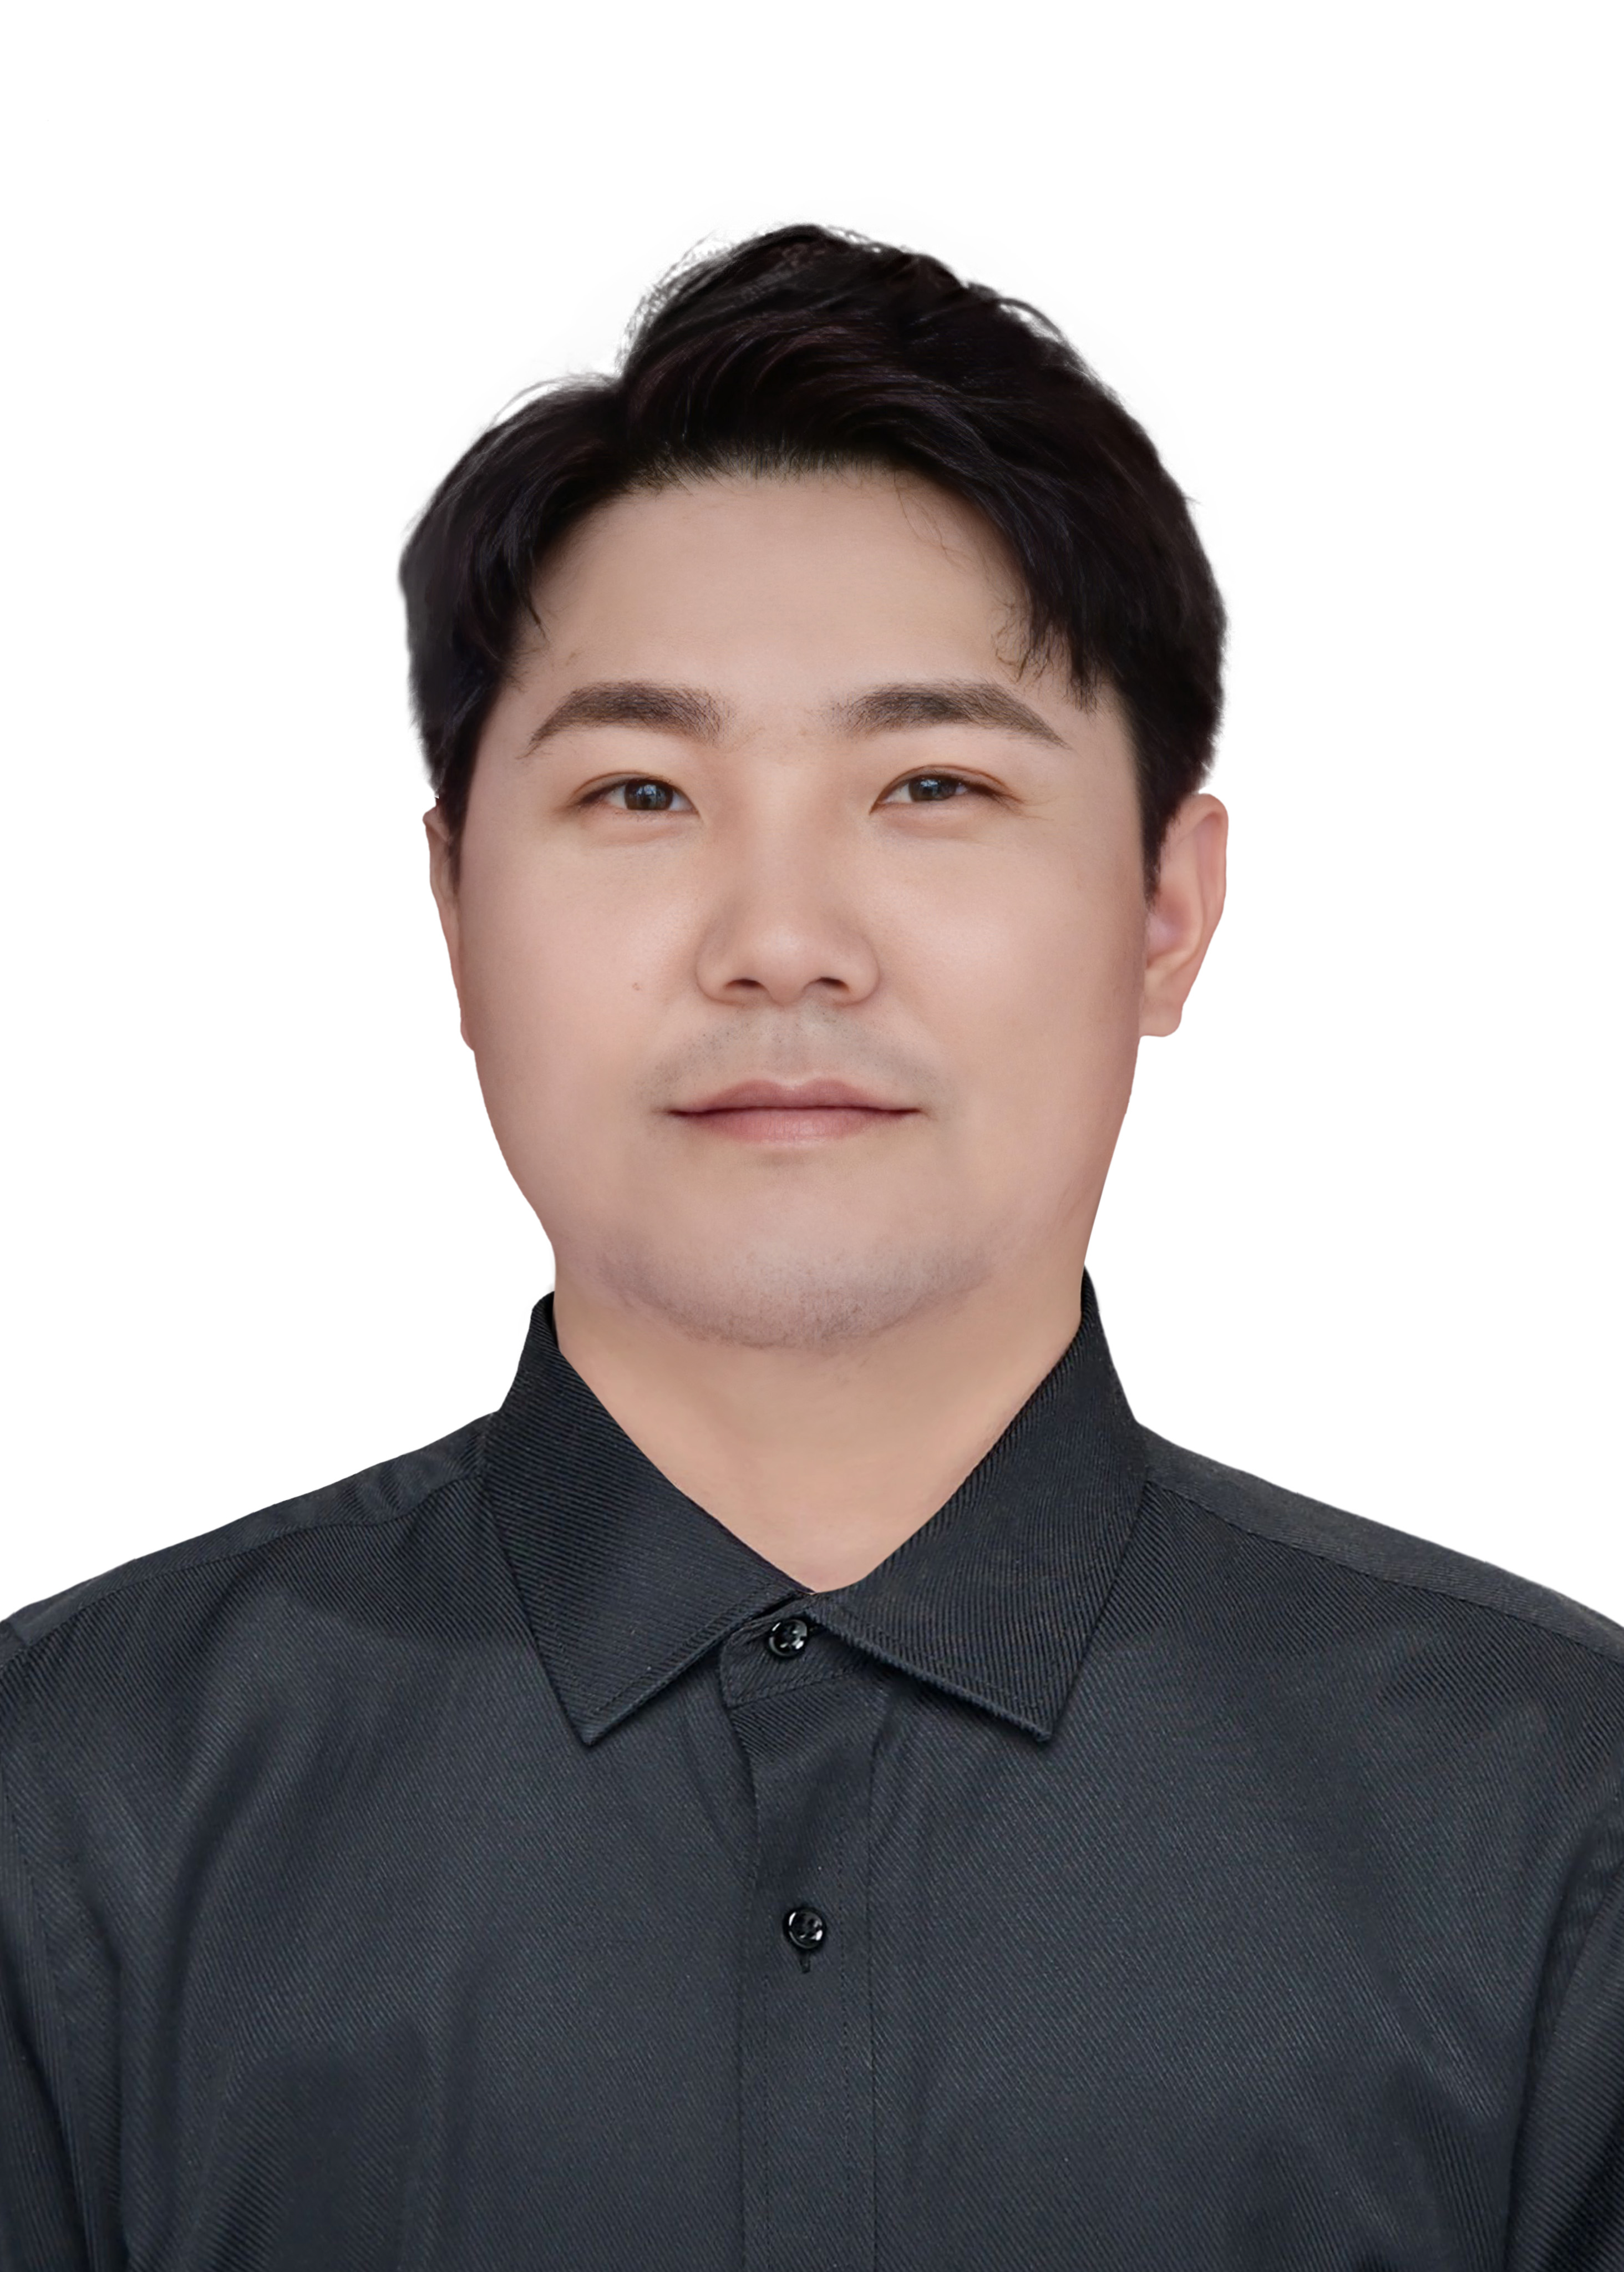
\includegraphics[width=1in,height=1.25in,clip,keepaspectratio]{Bio_picture/Qiquan_ZHANG.jpg}}]{Qiquan Zhang} (Member IEEE) received the B.Sc. and Ph.D. degrees in electronic science \& technology from Harbin Institute of Technology (HIT), China, in 2015 and 2020, respectively. From 2021 to 2022, he was a Postdoctoral Research Fellow with the Human Language Technology (HLT) Lab in the Department of Electrical and Computer Engineering, National University of Singapore (NUS) under the supervision of Prof. Haizhou Li. Since 2022, he has been a Research Associate with the Signal Processing Lab, The University of New South Wales (UNSW), Sydney, Australia, under the supervision of Prof. Eliathamby Ambikairajah and Prof. Haizhou Li. His research interests include statistical signal processing, speech processing, audio-visual speech processing, speech enhancement, noise estimation, machine learning, and deep learning.
% \end{IEEEbiography}

% \vspace{-0.6in}

% \begin{IEEEbiography}[{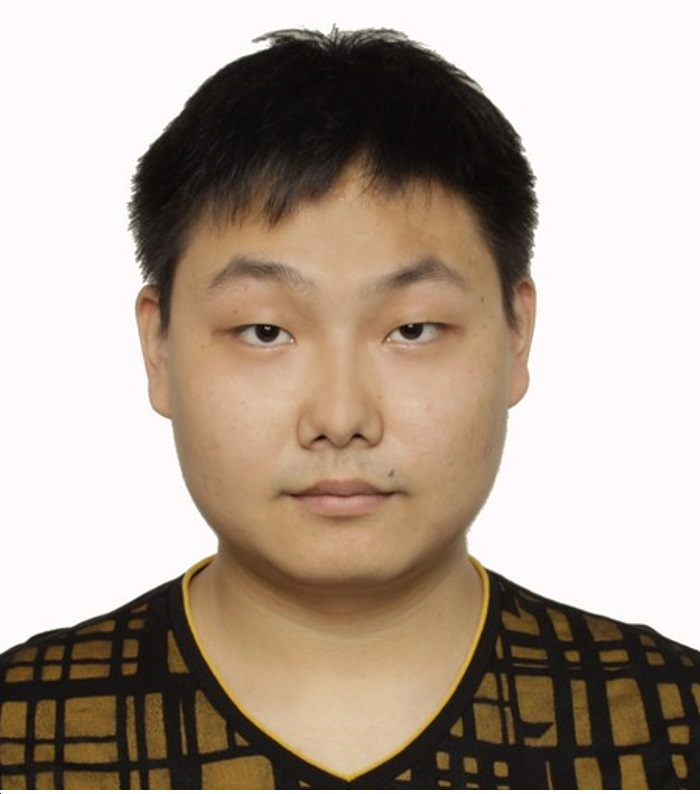
\includegraphics[width=1in,height=1.25in,clip,keepaspectratio]{Bio_picture/Hongxu_Zhu.jpg}}]{Hongxu Zhu} (Member IEEE) received his B.Sc. degree from Xi'an Jiaotong University in 2015 and received M.Sc. and Ph. D. degrees from City University of Hong Kong in 2017 and 2021, respectively. He is currently a Research Scientist in Fano, HongKong, China. Prior to this, he was a Lead Engineer at the Hong Kong Applied Science and Technology Research Institute (ASTRI). He also worked as a Research Fellow at the National University of Singapore, focusing on speech processing and brain-informed assistive hearing. He has published over 30 technical papers in high-impact journals and well-recognized conferences. His research interests include Internet-of-Things (IoT), speech processing, and brain-computer interface.
% \end{IEEEbiography}

% \vspace{-0.4in}

% \begin{IEEEbiography}
% [{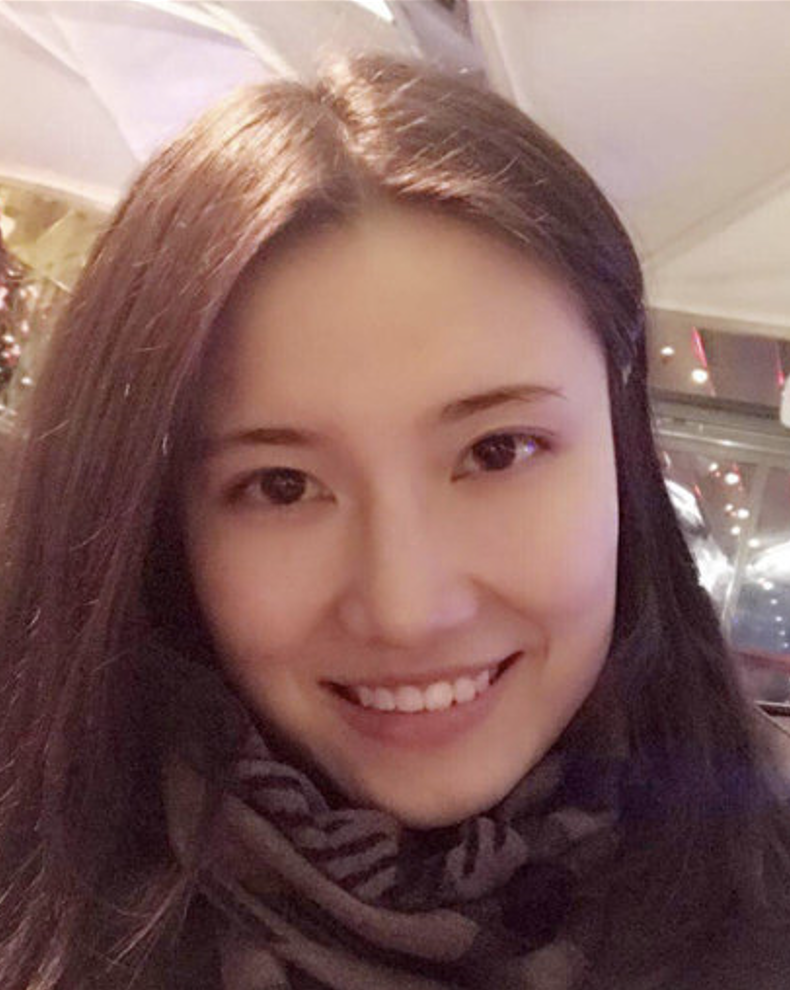
\includegraphics[width=1in,height=1.25in,clip,keepaspectratio]{Bio_picture/Xinyuan_Qian.png}}]{Xinyuan Qian} (Senior Member IEEE) received the B.Eng. (with First Class Hons.) and M.Sc. (with Distinction) degrees both from the University of Edinburgh, Edinburgh, U.K, She received the Ph.D. degree from Queen Mary, University of London, London, U.K.. She was a Research Fellow with National University of Singapore (NUS) from 2020 to 2022, and then became a visiting researcher with The Chinese University of Hong Kong, Shenzhen, China. She is currently an Associate Professor with the University of Science and Technology Beijing, China. Her research interests include speech processing, audio-visual sound localization, speech enhancement, and deep learning.
% \end{IEEEbiography}


% \begin{IEEEbiography}
% [{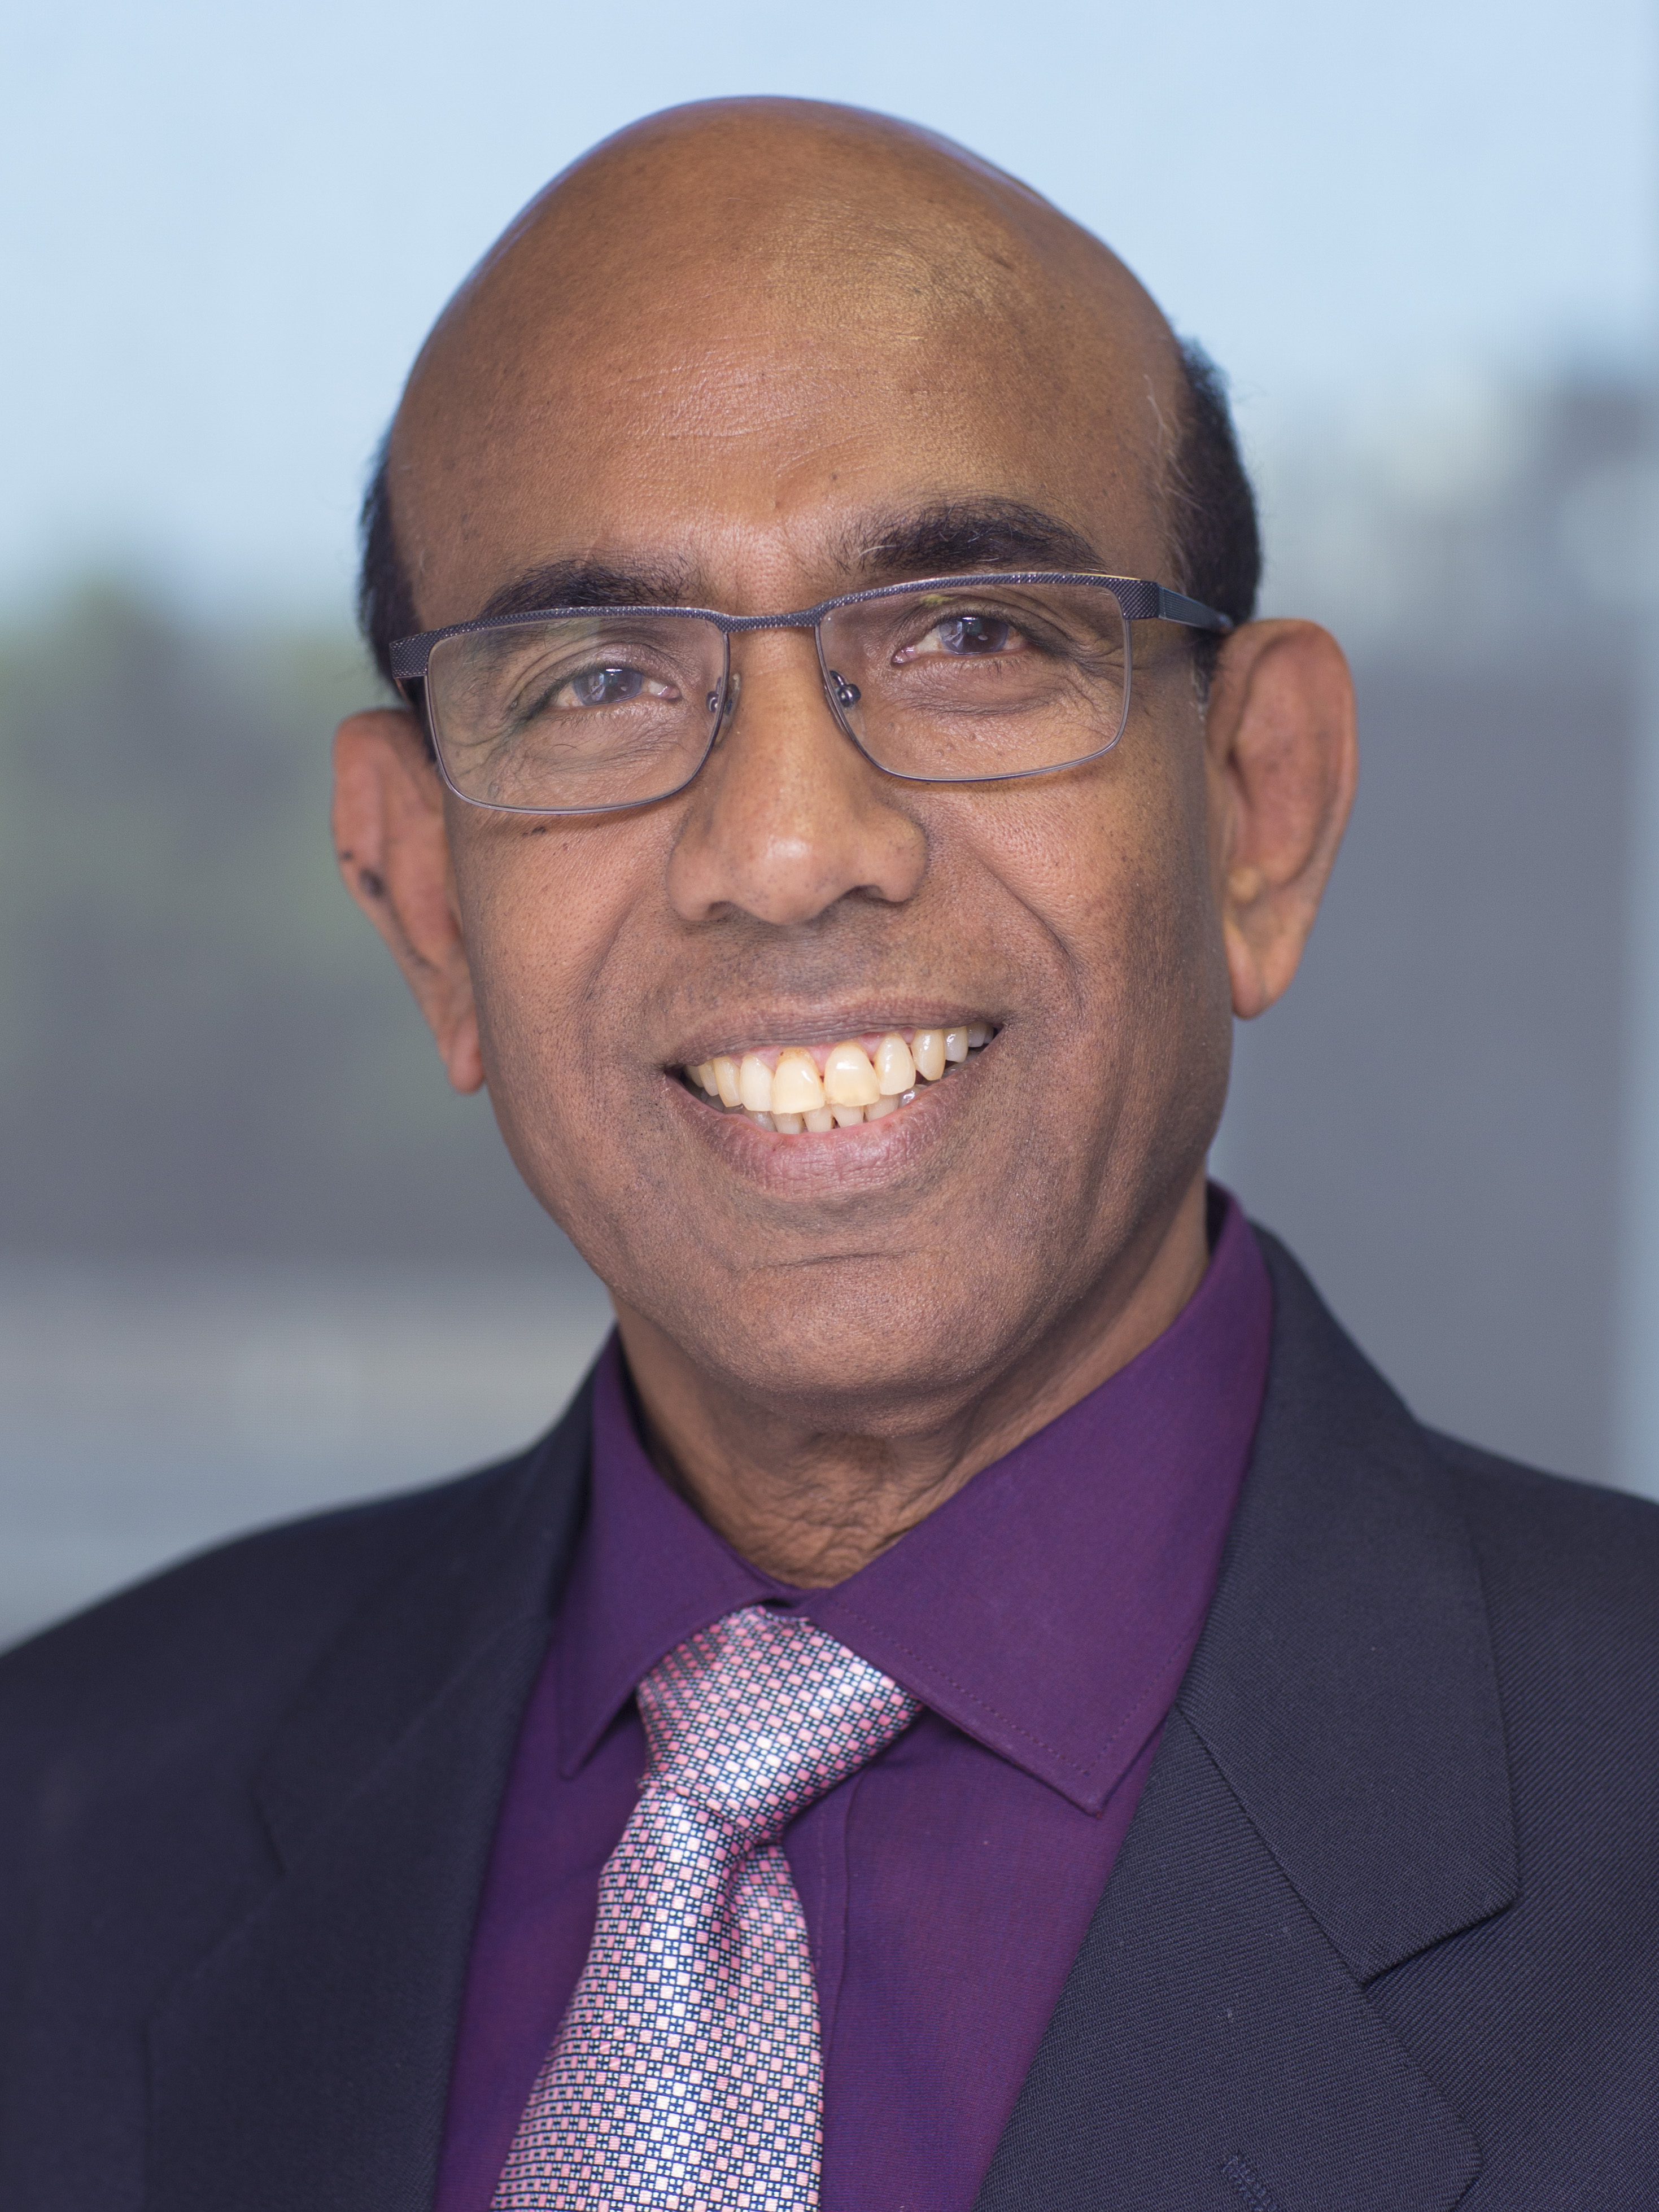
\includegraphics[width=1in,height=1.25in,clip,keepaspectratio]{Bio_picture/Eliathamby_Ambikairajah.jpg}}]
% {Eliathamby Ambikairajah} (Senior Member IEEE) received his BSc (Eng) (Hons) degree from the University of Sri Lanka, and received his PhD degree in Signal Processing from Keele University, UK. He was appointed as Head of Electronic Engineering and later Dean of Engineering at the Athlone Institute of Technology in the Republic of Ireland from 1982 to 1999. His key publications led to his repeated appointment as a short-term Invited Research Fellow with the British Telecom Laboratories, U.K., for ten years from 1989 to 1999. Professor Ambikairajah served as the Acting Deputy Vice-Chancellor Enterprise during 2020, after previously serving as the Head of School of Electrical Engineering and Telecommunications, University of New South Wales (UNSW), Australia from 2009 to 2019. His research interests include speaker and language recognition, emotion detection and biomedical signal processing. He has authored and co-authored approximately 300 journal and conference papers and is the recipient of many competitive research grants. He was a Faculty Associate with the Institute of Infocomm Research (A*STAR), Singapore from 2010 to 2018, and was an Advisory Board member of the AI Speech Lab at AI Singapore (2019-2021). Professor Ambikairajah was an Associate Editor for the IEEE Transactions on Education from 2012 to 2019. He received the UNSW Vice-Chancellor’s Award for Teaching Excellence in 2004 for his innovative use of educational technology and innovation in electrical engineering teaching programs, and in 2014 he received the UNSW Excellence in Senior Leadership Award. In 2019 was the recipient of the People’s Choice Award as part of the UNSW President’s Awards. Professor Ambikairajah was an APSIPA Distinguished Lecturer for the 2013-14 term. He is a Fellow and a Chartered Engineer of the IET UK and Engineers Australia (EA) and is a life Senior Member of the IEEE and a Life Member of APSIPA.
% \end{IEEEbiography}

% \begin{IEEEbiography}
% [{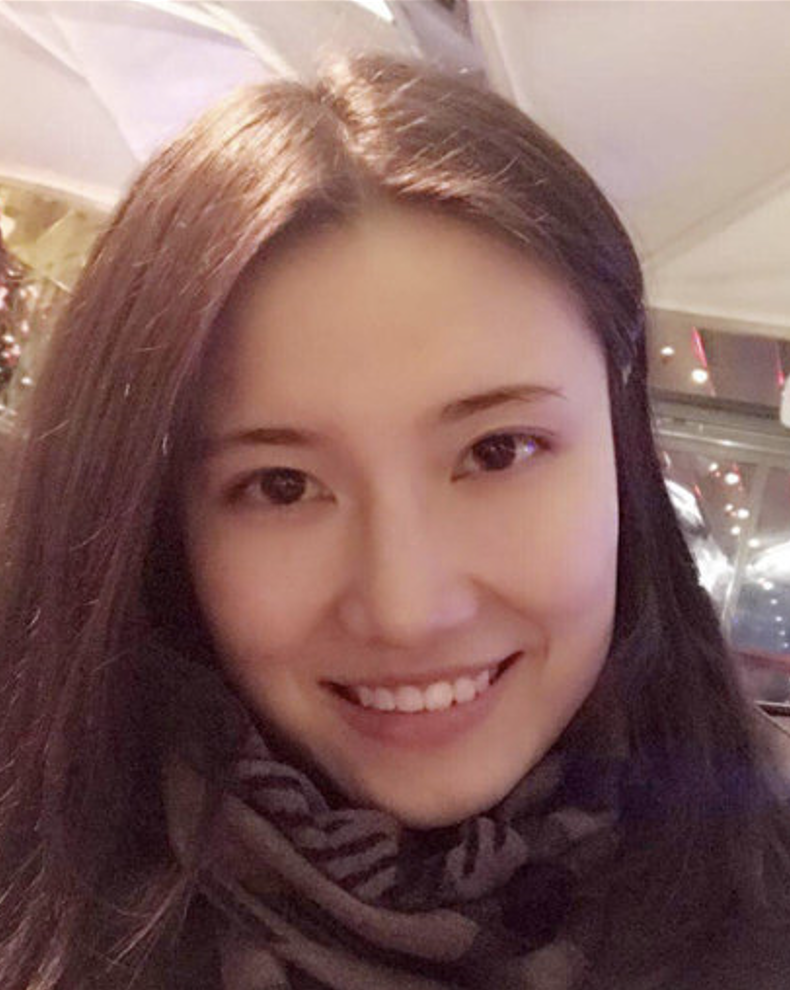
\includegraphics[width=1in,height=1.25in,clip,keepaspectratio]{Bio_picture/Xinyuan_Qian.png}}]{Xinyuan Qian} (Senior Member IEEE) received the B.Eng. (with First Class Hons.) and M.Sc. (with Distinction) degrees both from the University of Edinburgh, Edinburgh, U.K, She received the Ph.D. degree from Queen Mary, University of London, London, U.K.. She was a Research Fellow with National University of Singapore (NUS) from 2020 to 2022, and then became a visiting researcher with The Chinese University of Hong Kong, Shenzhen, China. She is currently an Associate Professor with the University of Science and Technology Beijing, China. Her research interests include speech processing, audio-visual sound localization, speech enhancement, and deep learning.
% \end{IEEEbiography}

% \vspace{-4.0in}

% \begin{IEEEbiography}
% [{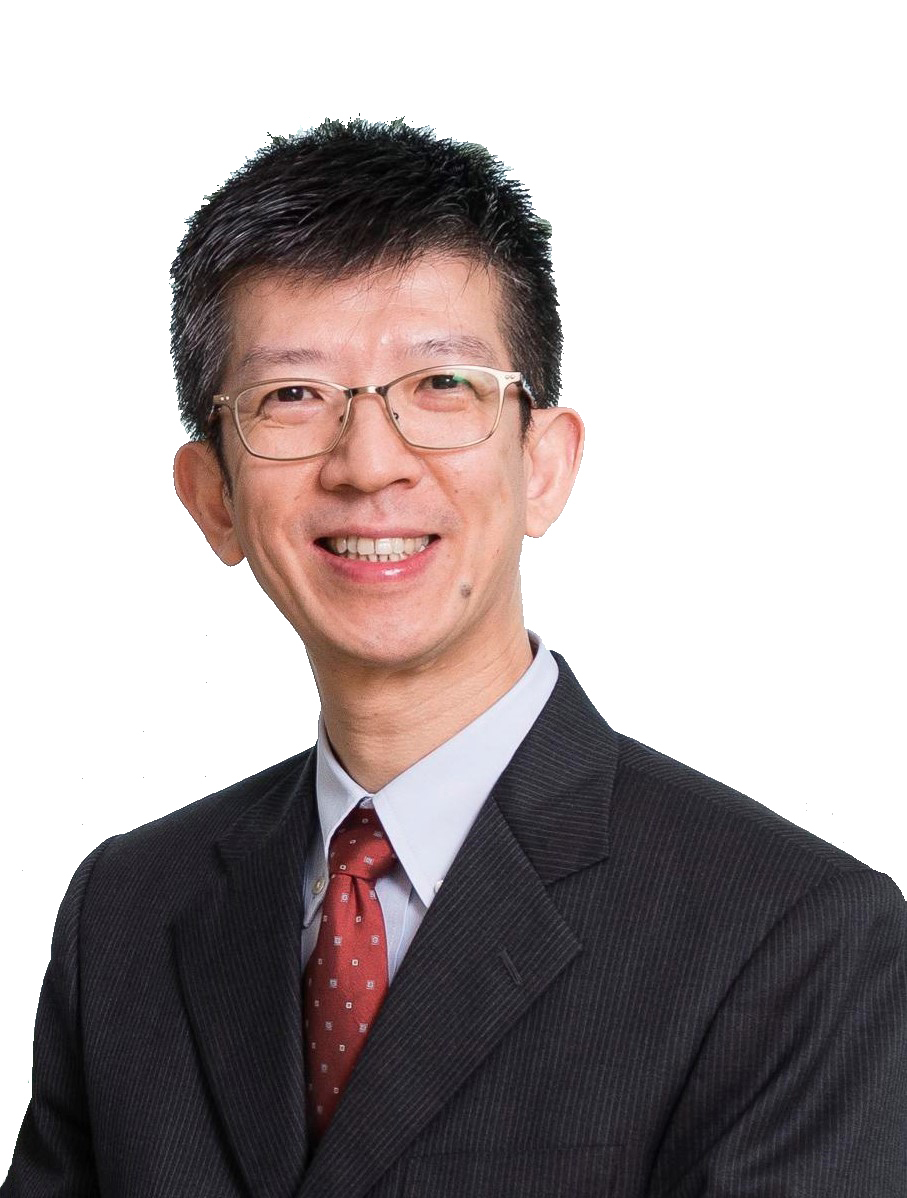
\includegraphics[width=1in,height=1.25in,clip,keepaspectratio]{Bio_picture/Haizhou_Li.jpg}}]
% {Haizhou Li} (Fellow, IEEE) received the B.Sc., M.Sc., and Ph.D. degrees in electrical and electronic engineering from South China University of Technology, Guangzhou, China in 1984, 1987, and 1990 respectively. He is currently a Presidential Chair Professor with the School of Data Science, The Chinese University of Hong Kong, Shenzhen, China. He is also an Adjunct Professor with the Department of Electrical and Computer Engineering, National University of Singapore (NUS). Prior to that, he taught in the University of Hong Kong (1988-1990) and South China University of Technology (1990-1994). He was a Visiting Professor at CRIN in France (1994-1995), Research Manager at the AppleISS Research Centre (1996-1998), Research Director in Lernout \& Hauspie Asia Pacific (1999-2001), Vice President in InfoTalk Corp. Ltd. (2001-2003), and the Principal Scientist and Department Head of Human Language Technology in the Institute for Infocomm Research, Singapore (2003-2016). His research interests include automatic speech recognition, speaker and language recognition, and natural language processing. Dr Li was the Editor-in-Chief of IEEE/ACM Transactions on Audio, Speech and Language Processing (2015-2018), a Member of the Editorial Board of Computer Speech and Language since 2012, an elected Member of IEEE Speech and Language Processing Technical Committee (2013-2015), the President of the International Speech Communication Association (2015-2017), the President of Asia Pacific Signal and Information Processing Association (2015-2016), and the President of Asian Federation of Natural Language Processing (2017-2018). He was the General Chair of ACL 2012, INTERSPEECH 2014, ASRU 2019 and ICASSP 2022. Dr Li is a Fellow of the ISCA, and a Fellow of the Academy of Engineering Singapore. He was the recipient of the National Infocomm Award 2002, and the President’s Technology Award 2013 in Singapore. He was named one of the two Nokia Visiting Professors in 2009 by the Nokia Foundation, and U Bremen Excellence Chair Professor in 2019.
% % \end{IEEEbiographynophoto}
% \end{IEEEbiography}

% if you will not have a photo at all:
% \vspace{-5mm} 
% \begin{IEEEbiographynophoto}{Qiquan Zhang} (Member IEEE) 
% received the B.Sc. and Ph.D degrees in electronic science \& technology from Harbin Institute of Technology, China, in 2015 and 2020, respectively. He is currently a postdoctoral research fellow with the Human Language Technology Lab in Department of Electrical and Computer Engineering, National University of Singapore, Singapore. His research interests include digital signal processing, speech processing, speech enhancement, noise estimation, machine learning and deep learning.
% \end{IEEEbiographynophoto}

% \vspace{-5mm}
% \begin{IEEEbiographynophoto}{Xinyuan Qian} (Member IEEE) 
% received the B.Eng. (with First Class Hons.) and M.Sc. (with Distinction) degrees both from the University of Edinburgh, Edinburgh, U.K, She received the Ph.D. degree from Queen Mary, University of London, London, U.K.. She has been a research fellow in National University of Singapore since Feb 2020 and then become a visiting researcher in Chinese University of Hong Kong (Shenzhen).
% \end{IEEEbiographynophoto}
% \vspace{-5mm}
% \begin{IEEEbiographynophoto}{Zhaoheng Ni}
% received the B.Sc. degree in Biology and Medical Engineering from Beihang University and M.S.c degree in Computer Science from City University of New York. He is currently a Research Scientist at Meta AI, United States. His research interests include single-channel and multi-channel speech enhancement, speech separation and Automatic Speech Recognition.
% \end{IEEEbiographynophoto}
% \vspace{-5mm}
% \begin{IEEEbiographynophoto}{Aaron Nicolson} He received his BEng degree (Class 1A Hons.) from Griffith University, in 2016. In 2020, he completed his PhD at the Signal Processing Laboratory of Griffith University, Brisbane, Australia under the supervision of Kuldip K. Paliwal. He is a postdoctoral research fellow at the Commonwealth Scientific and Industrial Research Organisation (CSIRO), stationed at the Australia e-Health Research Centre in Brisbane, Australia, since 2020. He is also a part of CSIRO's machine learning \& Artificial Intelligence Future Science Platform. His research interests include speech processing, speech enhancement, and medical image analysis.
% \end{IEEEbiographynophoto}
% \vspace{-5mm} 
% \begin{IEEEbiographynophoto}{Eliathamby Ambikairajah} (Senior Member IEEE) received his BSc (Eng) (Hons) degree from the University of Sri Lanka, and received his PhD degree in Signal Processing from Keele University, UK. He was appointed as Head of Electronic Engineering and later Dean of Engineering at the Athlone Institute of Technology in the Republic of Ireland from 1982 to 1999. His key publications led to his repeated appointment as a short-term Invited Research Fellow with the British Telecom Laboratories, U.K., for ten years from 1989 to 1999. Professor Ambikairajah served as the Acting Deputy Vice-Chancellor Enterprise during 2020, after previously serving as the Head of School of Electrical Engineering and Telecommunications, University of New South Wales (UNSW), Australia from 2009 to 2019. His research interests include speaker and language recognition, emotion detection and biomedical signal processing. He has authored and co-authored approximately 300 journal and conference papers and is the recipient of many competitive research grants. He was a Faculty Associate with the Institute of Infocomm Research (A*STAR), Singapore from 2010 to 2018, and was an Advisory Board member of the AI Speech Lab at AI Singapore (2019-2021). Professor Ambikairajah was an Associate Editor for the IEEE Transactions on Education from 2012 to 2019. He received the UNSW Vice-Chancellor’s Award for Teaching Excellence in 2004 for his innovative use of educational technology and innovation in electrical engineering teaching programs, and in 2014 he received the UNSW Excellence in Senior Leadership Award. In 2019 was the recipient of the People’s Choice Award as part of the UNSW President’s Awards. Professor Ambikairajah was an APSIPA Distinguished Lecturer for the 2013-14 term. He is a Fellow and a Chartered Engineer of the IET UK and Engineers Australia (EA) and is a life Senior Member of the IEEE and a Life Member of APSIPA.
% \end{IEEEbiographynophoto}
% \vspace{-5mm}
% \begin{IEEEbiographynophoto}{Haizhou Li} (Fellow, IEEE) received the B.Sc., M.Sc., and Ph.D. degree in electrical and electronic engineering from South China University of Technology, Guangzhou, China in 1984, 1987, and 1990 respectively. He is currently a Presidential Chair Professor with the School of Data Science, The Chinese University of Hong Kong, Shenzhen, China. He is also an Adjunct Professor with the Department of Electrical and Computer Engineering, National University of Singapore (NUS). Prior to that, he taught in the University of Hong Kong (1988-1990) and South China University of Technology (1990-1994). He was a Visiting Professor at CRIN in France (1994-1995), Research Manager at the AppleISS Research Centre (1996-1998), Research Director in Lernout \& Hauspie Asia Pacific (1999-2001), Vice President in InfoTalk Corp. Ltd. (2001-2003), and the Principal Scientist and Department Head of Human Language Technology in the Institute for Infocomm Research, Singapore (2003-2016). His research interests include automatic speech recognition, speaker and language recognition, natural language processing. Dr Li was the Editor-in-Chief of IEEE/ACM Transactions on Audio, Speech and Language Processing (2015-2018), a Member of the Editorial Board of Computer Speech and Language since 2012, an elected Member of IEEE Speech and Language Processing Technical Committee (2013-2015), the President of the International Speech Communication Association (2015-2017), the President of Asia Pacific Signal and Information Processing Association (2015-2016), and the President of Asian Federation of Natural Language Processing (2017-2018). He was the General Chair of ACL 2012, INTERSPEECH 2014, ASRU 2019 and ICASSP 2022. Dr Li is a Fellow of the ISCA, and a Fellow of the Academy of Engineering Singapore. He was the recipient of the National Infocomm Award 2002, and the President’s Technology Award 2013 in Singapore. He was named one of the two Nokia Visiting Professors in 2009 by the Nokia Foundation, and U Bremen Excellence Chair Professor in 2019.
% \end{IEEEbiographynophoto}


% \begin{IEEEbiographynophoto}{John Doe}
% Biography text here.
% \end{IEEEbiographynophoto}

% Author contribution
% Qiquan Zhang: Idea, Writing - review & editing, Methodology, Software, Experiments, Data curation.
% Xinyuan Qian: Software, Experiments, Writing - review & editing.
% Zhaoheng Ni: Writing - review & editing.
% Aaron Nicolson: Writing - review & editing.
% Eliathamby Ambikairajah: Writing - review & editing, Supervision.
% Haizhou Li: Writing - review & editing, Supervision.
% All authors discussed the results and commented on the manuscript.

% insert where needed to balance the two columns on the last page with
% biographies
%\newpage

% \begin{IEEEbiographynophoto}{Jane Doe}
% Biography text here.
% \end{IEEEbiographynophoto}

% You can push biographies down or up by placing
% a \vfill before or after them. The appropriate
% use of \vfill depends on what kind of text is
% on the last page and whether or not the columns
% are being equalized.

%\vfill

% Can be used to pull up biographies so that the bottom of the last one
% is flush with the other column.
%\enlargethispage{-5in}



% that's all folks
\end{document}


